%=========================
% main.tex
% Template LaTeX HCMUT - báo cáo đồ án tốt nghiệp
% Cấu trúc nội dung đã được map theo mục lục yêu cầu.
% Compile: pdfLaTeX -> Biber -> pdfLaTeX -> pdfLaTeX
%=========================
\documentclass[a4paper,12pt]{article}

%========== Cấu hình ==========
%=========================
% Preamble/packages.tex
% Bộ package nền tảng cho báo cáo đồ án Công nghệ phần mềm
% Ưu tiên tương thích Overleaf + pdfLaTeX + tiếng Việt.
%=========================

%========== Ngôn ngữ & mã hóa: pdfLaTeX + tiếng Việt ==========
\usepackage[T5]{fontenc}
\usepackage[utf8]{inputenc}
\usepackage[vietnamese]{babel}
\usepackage{lmodern}
\usepackage{microtype}
\usepackage{todonotes}
\usepackage{tabularx}

%========== Màu: nạp sớm để tránh option clash ==========
\usepackage[dvipsnames,table]{xcolor}
\definecolor{HCMUTBlue}{HTML}{005BAA}
\definecolor{HCMUTDarkBlue}{HTML}{003B73}
\definecolor{HCMUTLightBlue}{HTML}{EAF4FF}
\definecolor{SoftGray}{HTML}{F5F7FA}
\definecolor{BorderGray}{HTML}{D9E2EC}
\definecolor{CodeBg}{HTML}{F7F7F7}
\definecolor{CodeKeyword}{HTML}{005BAA}
\definecolor{CodeComment}{HTML}{5C6773}
\definecolor{CodeString}{HTML}{A31515}
\definecolor{SuccessGreen}{HTML}{EAF8EF}
\definecolor{WarningYellow}{HTML}{FFF7E6}
\definecolor{DangerRed}{HTML}{FDECEC}

%========== Bố cục trang ==========
\usepackage{geometry}
\geometry{
  a4paper,
  left=25mm,
  right=25mm,
  top=30mm,
  bottom=25mm,
  headheight=15pt
}
\usepackage{setspace}
\usepackage{indentfirst}
\usepackage{fancyhdr}
\usepackage{titlesec}
\usepackage{tocloft}


%========== Hình ảnh, biểu đồ, sơ đồ ==========
\usepackage{svg}
\usepackage{graphicx}
\graphicspath{{Images/}}
\usepackage{float}
\usepackage{subcaption}
\usepackage{caption}
\usepackage{wrapfig}
\usepackage{pdflscape}
\usepackage{adjustbox}
\usepackage{placeins}
\usepackage{pdfpages}
\usepackage{tikz}
\usetikzlibrary{arrows.meta,positioning,shapes.geometric,fit,backgrounds,calc,matrix}
\usepackage{pgfplots}
\pgfplotsset{compat=1.18}

%========== Toán, đơn vị, ký hiệu ==========
\usepackage{amsmath,amssymb,mathtools}
\usepackage{siunitx}

%========== Bảng chuyên nghiệp ==========
\usepackage{booktabs}
\usepackage{array}
\usepackage{tabularx}
\usepackage{longtable}
% Cho phép các cột kiểu X của tabularx ngắt qua nhiều trang.
\usepackage{ltablex}
\keepXColumns
\usepackage{multirow}
\usepackage{makecell}
\usepackage{colortbl}
\usepackage{threeparttable}
\usepackage{diagbox}
\usepackage{makecell}


\usepackage{array}
\usepackage{makecell}
\usepackage{ragged2e}
\usepackage{seqsplit}

%========== Danh sách, trích dẫn, ghi chú ==========
\usepackage{enumitem}
\usepackage[babel,strict=false]{csquotes}
\usepackage[most]{tcolorbox}

%========== Thuật toán / giả mã ==========
\usepackage{algorithm}
\usepackage{algpseudocode}

%========== Kế hoạch / tiến độ ==========
\usepackage{pgfgantt}

%========== Phụ lục ==========
\usepackage[toc,page]{appendix}

%========== URL ==========
\usepackage{xurl}
% Lưu ý: hyperref được nạp trong Preamble/style.tex sau biblatex để giảm xung đột.


%%% bìa
\usepackage{tikz}

%=========================
% Preamble/metadata.tex
% Chỉnh thông tin báo cáo tại đây để bìa tự cập nhật
%=========================

\newcommand{\UniversityName}{ĐẠI HỌC QUỐC GIA THÀNH PHỐ HỒ CHÍ MINH}
\newcommand{\SchoolName}{TRƯỜNG ĐẠI HỌC BÁCH KHOA}
\newcommand{\FacultyName}{KHOA KHOA HỌC VÀ KỸ THUẬT MÁY TÍNH}

\newcommand{\ReportHeading}{BÁO CÁO}
\newcommand{\ReportType}{ĐỒ ÁN TỐT NGHIỆP}
\newcommand{\ProjectTitleMain}{Xây dựng Trợ lý Mua sắm Đa phương tiện sử dụng RAG và Computer Vision}
% \newcommand{\ProjectTitleSub}{(Multimodal AI Shopping Assistant) cho hệ thống thương mại điện tử}
\newcommand{\MajorLabel}{Ngành:}
\newcommand{\MajorName}{Khoa học Máy tính}
\newcommand{\CouncilLabel}{HỘI ĐỒNG:}
\newcommand{\CouncilName}{}
\newcommand{\AdvisorLabel}{GVHD:}
\newcommand{\AdvisorName}{ThS.~Võ Thanh Hùng}
\newcommand{\ReviewerLabel}{GVPB:}
\newcommand{\ReviewerName}{}

\newcommand{\StudentOne}{Lê Trần Anh Dũng -- 2210576}
\newcommand{\StudentTwo}{Huỳnh Thái Minh Châu -- 2210352}
\newcommand{\StudentThree}{Nguyễn Đức Duy -- 2210510}

\newcommand{\ReportPlaceDate}{TP. Hồ Chí Minh, Tháng 9/2026}
\newcommand{\LogoFile}{hcmut.png}

% Metadata cho PDF
\newcommand{\ReportTitle}{\ProjectTitleMain}
\newcommand{\ReportAuthors}{Lê Trần Anh Dũng, Huỳnh Thái Minh Châu, Nguyễn Đức Duy}

%=========================
% Preamble/listings.tex
% Cấu hình hiển thị mã nguồn, phù hợp báo cáo Công nghệ phần mềm
% Không dùng minted để tránh yêu cầu shell-escape.
%=========================

\usepackage{listings}

\renewcommand{\lstlistingname}{Mã nguồn}
\renewcommand{\lstlistlistingname}{Danh mục mã nguồn}

\lstdefinestyle{pretty}{
  backgroundcolor=\color{CodeBg},
  basicstyle=\ttfamily\small,
  keywordstyle=\color{CodeKeyword}\bfseries,
  commentstyle=\color{CodeComment}\itshape,
  stringstyle=\color{CodeString},
  numbers=left,
  numberstyle=\tiny\color{CodeComment},
  stepnumber=1,
  numbersep=8pt,
  breaklines=true,
  breakatwhitespace=false,
  frame=single,
  rulecolor=\color{BorderGray},
  showstringspaces=false,
  tabsize=2,
  columns=fullflexible,
  keepspaces=true,
  captionpos=b
}

\lstdefinestyle{terminal}{
  backgroundcolor=\color{black!92},
  basicstyle=\ttfamily\small\color{white},
  numbers=none,
  frame=single,
  rulecolor=\color{black!70},
  breaklines=true,
  showstringspaces=false,
  tabsize=2,
  columns=fullflexible
}

\lstdefinelanguage{JavaScript}{
  keywords={const,let,var,function,return,async,await,if,else,for,while,try,catch,throw,new,class,extends,import,from,export,default},
  sensitive=true,
  comment=[l]{//},
  morecomment=[s]{/*}{*/},
  morestring=[b]',
  morestring=[b]",
  morestring=[b]`
}

\lstdefinelanguage{JSON}{
  morestring=[b]",
  stringstyle=\color{CodeString},
  literate=
   *{0}{{{0}}}{1} {1}{{{1}}}{1} {2}{{{2}}}{1} {3}{{{3}}}{1} {4}{{{4}}}{1}
    {5}{{{5}}}{1} {6}{{{6}}}{1} {7}{{{7}}}{1} {8}{{{8}}}{1} {9}{{{9}}}{1}
    {:}{{{\color{CodeKeyword}{:}}}}{1} {,}{{{\color{CodeKeyword}{,}}}}{1}
    {\{}{{{\color{CodeKeyword}{\{}}}}{1} {\}}{{{\color{CodeKeyword}{\}}}}}{1}
    {[}{{{\color{CodeKeyword}{[}}}}{1} {]}{{{\color{CodeKeyword}{]}}}}{1}
}

\lstdefinelanguage{Dockerfile}{
  keywords={FROM,RUN,COPY,ADD,WORKDIR,CMD,ENTRYPOINT,ENV,EXPOSE,ARG,VOLUME,USER,LABEL},
  sensitive=true,
  comment=[l]{\#},
  morestring=[b]"
}

\lstset{style=pretty}


%=========================
% Preamble/bibliography.tex
% IEEE: biblatex + biber
%=========================

\usepackage{csquotes}
\usepackage{xurl}

\DeclareQuoteStyle{vietnamese}
  {\textquotedblleft}
  {\textquotedblright}
  {\textquoteleft}
  {\textquoteright}

\usepackage[
  backend=biber,
  style=ieee,
  sorting=none,
  language=vietnamese,
  autolang=other,
  url=true,
  doi=true,
  isbn=false
]{biblatex}

\AtBeginBibliography{\sloppy}
\addbibresource{References/refs.bib}
%=========================
% Preamble/style.tex
% Style chung: màu sắc, header/footer, caption, box, hyperlink, clever reference
%=========================

%========== Tên thành phần tiếng Việt ==========
\renewcommand{\contentsname}{Mục lục}
\renewcommand{\listfigurename}{Danh mục hình}
\renewcommand{\listtablename}{Danh mục bảng}
\renewcommand{\figurename}{Hình}
\renewcommand{\tablename}{Bảng}
\renewcommand{\refname}{Tài liệu tham khảo}
\floatname{algorithm}{Thuật toán}
\renewcommand{\algorithmicrequire}{\textbf{Đầu vào:}}
\renewcommand{\algorithmicensure}{\textbf{Đầu ra:}}

%========== Typography & paragraph ==========
\onehalfspacing
\setlength{\parindent}{1.2cm}
\setlength{\parskip}{3pt}
\setlist{itemsep=3pt, topsep=4pt}
\renewcommand{\arraystretch}{1.18}
\setlength{\tabcolsep}{4pt}

%========== Header / footer ==========
\pagestyle{fancy}
\fancyhf{}
\lhead{
\includegraphics[height=10mm]{Images/coverpage/bk_name_vi.png}}
\rhead{\small \nouppercase{\leftmark}}
\cfoot{\thepage}
\setlength{\headheight}{33pt}
\renewcommand{\headrulewidth}{0.4pt}
\renewcommand{\footrulewidth}{0pt}

%========== Tiêu đề kiểu chương trong article ==========
% Section vẫn đánh số 1, 2, 3 để subsection là 1.1, 1.2...
% Nhưng heading hiển thị là "Chương 1 -- Tên chương".
\titleformat{\section}
  {\clearpage\Large\bfseries\color{HCMUTDarkBlue}}
  {Chương~\thesection}{0.8em}{--\ }
\titleformat{\subsection}
  {\large\bfseries\color{HCMUTBlue}}
  {\thesubsection}{0.8em}{}
\titleformat{\subsubsection}
  {\normalsize\bfseries\color{HCMUTDarkBlue}}
  {\thesubsubsection}{0.8em}{}
\titlespacing*{\section}{0pt}{0pt}{10pt}
\titlespacing*{\subsection}{0pt}{12pt}{6pt}
\titlespacing*{\subsubsection}{0pt}{10pt}{4pt}

%========== Mục lục ==========
\renewcommand{\cftsecleader}{\cftdotfill{\cftdotsep}}
\setlength{\cftbeforesecskip}{4pt}

%========== Caption ==========
\captionsetup{
  labelfont={bf,color=HCMUTDarkBlue},
  textfont=it,
  font=small,
  justification=centering
}
\captionsetup[table]{position=top}

%========== Link ==========
\usepackage[unicode]{hyperref}
\hypersetup{
  colorlinks=true,
  linkcolor=HCMUTDarkBlue,
  citecolor=HCMUTDarkBlue,
  urlcolor=HCMUTBlue,
  filecolor=HCMUTBlue
}
\usepackage{bookmark}
\usepackage[nameinlink,noabbrev]{cleveref}

% Tên tham chiếu tiếng Việt cho cleveref.
\crefname{section}{chương}{chương}
\Crefname{section}{Chương}{Chương}
\crefname{subsection}{mục}{mục}
\Crefname{subsection}{Mục}{Mục}
\crefname{subsubsection}{mục}{mục}
\Crefname{subsubsection}{Mục}{Mục}
\crefname{figure}{hình}{hình}
\Crefname{figure}{Hình}{Hình}
\crefname{table}{bảng}{bảng}
\Crefname{table}{Bảng}{Bảng}
\crefname{algorithm}{thuật toán}{thuật toán}
\Crefname{algorithm}{Thuật toán}{Thuật toán}
\crefname{lstlisting}{mã nguồn}{mã nguồn}
\Crefname{lstlisting}{Mã nguồn}{Mã nguồn}

%========== tcolorbox: box dùng trong báo cáo ==========
\tcbset{
  enhanced,
  boxrule=0.6pt,
  arc=2mm,
  left=2mm,
  right=2mm,
  top=1.5mm,
  bottom=1.5mm,
  fonttitle=\bfseries,
  breakable
}

\newtcolorbox{infobox}[1]{
  title={#1},
  colback=HCMUTLightBlue,
  colframe=HCMUTBlue
}

\newtcolorbox{notebox}[1]{
  title={#1},
  colback=HCMUTLightBlue,
  colframe=HCMUTDarkBlue,
  coltitle=white,
  colbacktitle=HCMUTDarkBlue
}

\newtcolorbox{warningbox}[1]{
  title={#1},
  colback=WarningYellow,
  colframe=orange!70!black
}

\newtcolorbox{requirementbox}[1]{
  title={#1},
  colback=SuccessGreen,
  colframe=green!45!black
}

\newtcolorbox{riskbox}[1]{
  title={#1},
  colback=DangerRed,
  colframe=red!60!black
}

%========== Macro tiện ích ==========
\newcommand{\filepath}[1]{\texttt{\detokenize{#1}}}
\newcommand{\inlinecode}[1]{\texttt{\detokenize{#1}}}
\newcommand{\term}[1]{\textbf{#1}}
\newcommand{\todoitem}[1]{\textcolor{red!70!black}{\textbf{TODO:} #1}}
\newcommand{\sourceplaceholder}{\textcolor{red!70!black}{[Cần trích dẫn nguồn]}}


% Tạo heading không đánh số, không đưa vào mục lục, không hiện số trang.
\newcommand{\frontmatterchapter}[1]{%
  \clearpage
  \section*{#1}
  \thispagestyle{empty}
}

%========== Cấu hình siunitx ==========
\sisetup{
  detect-all,
  group-separator={,},
  group-minimum-digits=4
}

%feedback 
\newcommand{\commentlines}[1]{%
  \par\noindent
  \begingroup
  \color{black!35}%
  \count0=0
  \loop\ifnum\count0<#1
    \noindent\rule{\textwidth}{0.4pt}\par\vspace{0.75cm}%
    \advance\count0 by 1
  \repeat
  \endgroup
}

\hypersetup{
  pdftitle={\ReportTitle},
  pdfauthor={\ReportAuthors}
}
\begin{document}

%========== Bìa + phần đầu ==========
%=========================
% FrontMatter/cover.tex
% Bìa báo cáo, bố cục theo biểu mẫu LVTN/ĐATN của Khoa KH&KT Máy tính.
%=========================

\pagenumbering{gobble}
\thispagestyle{empty}

% Khung đôi của biểu mẫu: nét ngoài mảnh, khe hẹp, nét trong dày.
\begin{tikzpicture}[remember picture,overlay]
  \draw[line width=0.9pt]
    ([xshift=15mm,yshift=-15mm]current page.north west)
    rectangle
    ([xshift=-15mm,yshift=15mm]current page.south east);
  \draw[line width=2.7pt]
    ([xshift=16mm,yshift=-16mm]current page.north west)
    rectangle
    ([xshift=-16mm,yshift=16mm]current page.south east);
\end{tikzpicture}

\begingroup
\setlength{\parindent}{0pt}
\setlength{\parskip}{0pt}
% Làm chữ đậm hơn mức bold mặc định trên riêng trang bìa (pdfLaTeX).
\newcommand{\coverstrongstart}{%
  \pdfliteral direct {2 Tr 0.22 w}\bfseries}
\newcommand{\coverstrongend}{%
  \pdfliteral direct {0 Tr 0 w}}
\newcommand{\coverstrong}[1]{{\coverstrongstart #1\coverstrongend}}
\vspace*{-17mm}

% Tên đơn vị.
\begin{center}
  {\fontsize{15}{18}\selectfont
    \coverstrong{\UniversityName}\par
    \coverstrong{\SchoolName}\par
    \coverstrong{\FacultyName}\par}
\end{center}

\vspace{5mm}

% Logo trường.
\begin{center}
  \IfFileExists{Images/\LogoFile}{%
    \includegraphics[
      width=31mm,
      trim=226bp 126bp 219bp 69bp,
      clip
    ]{\LogoFile}%
  }{%
    \fbox{\parbox[c][25mm][c]{36mm}{\centering LOGO TRƯỜNG}}%
  }
\end{center}

\vspace{5mm}

% Loại báo cáo/môn học.
\begin{center}
  {\fontsize{15}{18}\selectfont\bfseries
    \coverstrong{\ReportHeading}\par
    \coverstrong{\ReportType}\par}
\end{center}

\vspace{4mm}

% Tên đề tài.
\begin{center}
  \begin{minipage}{0.88\textwidth}
    \centering
    {\fontsize{20}{24}\selectfont
      \coverstrong{\MakeUppercase{\ProjectTitleMain}}\par}
  \end{minipage}
\end{center}

\vspace{7mm}

% Ngành đào tạo.
\begin{center}
  {\fontsize{13.5}{17}\selectfont
    \textbf{\MajorLabel}~\MajorName\par}
\end{center}

\vfill

% Thông tin hội đồng, giảng viên và sinh viên được đặt lệch phải như biểu mẫu.
\noindent\hspace*{31mm}%
\begin{minipage}{125mm}
  \fontsize{13.5}{17}\selectfont
  \begin{tabular}{@{}>{\bfseries}p{36mm}@{}p{87mm}@{}}
    \CouncilLabel  & \CouncilName \\
    \AdvisorLabel  & \hspace*{-11mm}\AdvisorName \\
    \ReviewerLabel & \ReviewerName
  \end{tabular}

  \vspace{1mm}
  \begin{center}
    \textbf{---o0o---}
  \end{center}
  \vspace{1mm}

  \begin{tabular}{@{}>{\bfseries}p{25mm}@{}p{98mm}@{}}
    SVTH 1: & \StudentOne \\
    SVTH 2: & \StudentTwo \\
    SVTH 3: & \StudentThree
  \end{tabular}
\end{minipage}

\vspace{6mm}
\vfill

\begin{center}
  {\fontsize{13.5}{17}\selectfont\textbf{\ReportPlaceDate}}
\end{center}

\vspace*{2mm}
\endgroup

\clearpage

%=========================
% FrontMatter/lists.tex
% Thứ tự phần đầu theo yêu cầu báo cáo
%=========================

% Các trang chữ ký, cam đoan, cảm ơn, tóm tắt và mục lục không đánh số.
\pagenumbering{gobble}
\pagestyle{empty}


%=========================
% FrontMatter/advisor_signature.tex
% Trang chữ ký của giảng viên hướng dẫn
%=========================
\clearpage
\thispagestyle{empty}

\begin{center}
    \textbf{\LARGE CHỮ KÝ GIẢNG VIÊN HƯỚNG DẪN}
\end{center}

\vspace{5.2cm}

\noindent
\hspace{0.9cm}%
\rule{0.50\textwidth}{0.4pt}%
\hspace{0.4cm}%
\textit{Ngày}%
\hspace{0.4cm}%
\rule{0.25\textwidth}{0.4pt}

\vspace{1.1cm}

\noindent
\textbf{ThS. VÕ THANH HÙNG}\\
\textbf{KHOA KHOA HỌC VÀ KỸ THUẬT MÁY TÍNH}

\clearpage

\newpage
\begin{center}
    \textbf{\Large LỜI CAM ĐOAN}
\end{center}

Chúng em xin cam đoan đồ án tốt nghiệp với đề tài
\textit{\enquote{\textbf{Xây dựng Trợ lý Mua sắm Đa phương tiện sử dụng RAG và Computer Vision}}}
là kết quả của quá trình học tập, nghiên cứu và phát triển do nhóm trực tiếp thực hiện dưới sự hướng dẫn của ThS.~Võ Thanh Hùng. Các nội dung trong báo cáo phản ánh đúng quá trình nhóm phân tích yêu cầu, thiết kế, xây dựng, triển khai và đánh giá hệ thống.

Các kết quả thực nghiệm, hình ảnh minh họa và nhận xét được trình bày trung thực trong phạm vi dữ liệu và môi trường thử nghiệm của đồ án. Nhóm không cố ý điều chỉnh, che giấu hoặc diễn giải sai lệch kết quả nhằm làm thay đổi bản chất của quá trình đánh giá. Những hạn chế còn tồn tại của hệ thống cũng được ghi nhận trong báo cáo để bảo đảm tính khách quan.

Trong quá trình thực hiện, nhóm có tham khảo các tài liệu chuyên ngành, bài báo khoa học, tài liệu kỹ thuật và những nguồn thông tin phù hợp. Các nội dung kế thừa từ công trình của cá nhân hoặc tổ chức khác đều được ghi nhận và trích dẫn theo quy định học thuật. Nhóm cam kết không sao chép, không đạo văn và không sử dụng trái phép kết quả nghiên cứu của người khác.

Chúng em xin chịu trách nhiệm trước Khoa, Nhà trường và Hội đồng chấm đồ án về tính trung thực của nội dung được trình bày trong báo cáo này.

\vspace{1cm}

\par\hfill\textbf{Nhóm tác giả}

\par\hfill\textit{Lê Trần Anh Dũng}

\par\hfill\textit{Huỳnh Thái Minh Châu}

\par\hfill\textit{Nguyễn Đức Duy}
\newpage

\begin{center}
    \textbf{\Large LỜI CẢM ƠN}
\end{center}

Trước hết, tôi xin chân thành cảm ơn Ban Giám hiệu Trường Đại học Bách khoa, Đại học Quốc gia Thành phố Hồ Chí Minh đã tạo dựng môi trường học tập và nghiên cứu thuận lợi để tôi có cơ hội tiếp cận kiến thức chuyên môn, rèn luyện kỹ năng và thực hiện đồ án tốt nghiệp.

Tôi xin trân trọng cảm ơn Khoa Khoa học và Kỹ thuật Máy tính cùng quý thầy cô đã tận tình giảng dạy, truyền đạt những kiến thức nền tảng và chuyên ngành trong suốt quá trình học tập. Những kiến thức và kinh nghiệm được quý thầy cô chia sẻ là hành trang quan trọng, giúp tôi có cơ sở để nghiên cứu và xây dựng đề tài \textit{\enquote{\textbf{Xây dựng Trợ lý Mua sắm Đa phương tiện sử dụng RAG và Computer Vision}}}.

Đặc biệt, tôi xin bày tỏ lòng biết ơn sâu sắc đến ThS.~Võ Thanh Hùng, giảng viên trực tiếp hướng dẫn tôi. Trong suốt quá trình thực hiện đồ án, thầy đã tận tình định hướng, góp ý về phương pháp nghiên cứu, hỗ trợ chuyên môn và giúp tôi nhìn nhận rõ hơn những vấn đề còn hạn chế. Những nhận xét và chỉ dẫn của thầy đã giúp tôi từng bước hoàn thiện hệ thống và nâng cao chất lượng báo cáo.

Tôi trân trọng cảm ơn hai bạn Lê Trần Anh Dũng và Nguyễn Đức Duy vì những đóng góp, trao đổi và phối hợp trong giai đoạn thực hiện đồ án chuyên ngành, qua đó tạo tiền đề tham khảo hữu ích cho quá trình phát triển đồ án tốt nghiệp này.

Tôi cũng xin gửi lời cảm ơn đến gia đình và bạn bè đã luôn động viên, chia sẻ và hỗ trợ trong quá trình học tập cũng như thực hiện đồ án. Sự quan tâm và khích lệ của mọi người là nguồn động lực để tôi vượt qua những khó khăn và hoàn thành công việc của mình.

Mặc dù đã nỗ lực thực hiện đồ án với tinh thần nghiêm túc và trách nhiệm, do giới hạn về thời gian, kinh nghiệm và phạm vi nghiên cứu, báo cáo khó tránh khỏi những thiếu sót. Tôi rất mong nhận được các ý kiến nhận xét và góp ý từ quý thầy cô để báo cáo và hệ thống tiếp tục được hoàn thiện.

Tôi xin chân thành cảm ơn.

\vspace{1cm}

\par\hfill\textbf{Tác giả}

\par\hfill\textit{Huỳnh Thái Minh Châu}
\newpage

%=========================
% FrontMatter/summary_vi.tex
% Tóm tắt báo cáo bằng tiếng Việt
%=========================
\begin{center}
    \textbf{\Large TÓM TẮT}
\end{center}

Đề tài \textit{\enquote{Xây dựng Trợ lý Mua sắm Đa phương tiện sử dụng RAG và Computer Vision}} hướng đến việc phát triển một nền tảng mua sắm trực tuyến thông minh, ứng dụng trí tuệ nhân tạo nhằm nâng cao khả năng tìm kiếm, tư vấn và lựa chọn sản phẩm trong lĩnh vực thương mại điện tử. Hệ thống được xây dựng như một nền tảng tích hợp, nơi người dùng có thể tra cứu thông tin sản phẩm, thực hiện các nghiệp vụ mua sắm và tương tác với trợ lý bằng ngôn ngữ tự nhiên hoặc hình ảnh.

Trong quá trình triển khai, đề tài tập trung hiện thực các chức năng cốt lõi gồm tìm kiếm sản phẩm bằng văn bản, tìm kiếm bằng hình ảnh, tìm kiếm kết hợp văn bản--hình ảnh và tư vấn sản phẩm qua hội thoại nhiều lượt. Trợ lý được phát triển dựa trên kỹ thuật Retrieval-Augmented Generation (RAG), mô hình ngôn ngữ lớn và bộ nhớ hội thoại nhằm khai thác dữ liệu sản phẩm được truy xuất, duy trì ngữ cảnh và tạo phản hồi phù hợp với yêu cầu của người dùng. Bên cạnh đó, các mô hình biểu diễn đa phương thức và kỹ thuật thị giác máy tính được sử dụng để trích xuất đặc trưng, hỗ trợ truy hồi những sản phẩm tương đồng với hình ảnh đầu vào.

Trong phạm vi báo cáo, tác giả trình bày quá trình phân tích, thiết kế, xây dựng và tích hợp các thành phần của hệ thống, bao gồm Frontend, Backend nghiệp vụ, cơ sở dữ liệu MySQL, AI Service và cơ sở dữ liệu vector Qdrant; đồng thời mô tả cơ chế đồng bộ và phối hợp giữa các thành phần nhằm bảo đảm tính nhất quán của dữ liệu.

Tôi cũng tiến hành đánh giá các cấu hình truy hồi, vai trò của RAG và bộ nhớ hội thoại, cùng với việc kiểm thử chức năng, hiệu năng, bảo mật và khả dụng của hệ thống. Kết quả cho thấy giải pháp có khả năng hỗ trợ người dùng tìm kiếm sản phẩm bằng nhiều phương thức, cung cấp phản hồi có căn cứ và duy trì ngữ cảnh hội thoại trong phạm vi thử nghiệm. Hệ thống thể hiện khả năng ứng dụng thực tiễn của trí tuệ nhân tạo trong việc hỗ trợ quá trình tìm kiếm và ra quyết định mua sắm, đồng thời tạo cơ sở để tiếp tục cải thiện chất lượng truy hồi, khả năng xử lý ràng buộc và trải nghiệm người dùng.


\clearpage
\phantomsection
\tableofcontents
\clearpage

% Bắt đầu dãy số La Mã từ Danh mục từ viết tắt và hiển thị ở chân trang.
\pagenumbering{roman}
\setcounter{page}{1}
\hypersetup{pageanchor=true}
\pagestyle{plain}

% Ghi các danh mục phần đầu vào mục lục kèm số trang La Mã.
\newcommand{\addfrontmattertoc}[1]{%
  \addcontentsline{toc}{section}{#1}%
}

\phantomsection
\addfrontmattertoc{Danh mục từ viết tắt}
%=========================
% FrontMatter/abbreviations.tex
% Danh mục từ viết tắt
%=========================

\frontmatterchapter{Danh mục từ viết tắt}
\begin{longtable}{|p{0.22\linewidth}|p{0.74\linewidth}|}
\caption*{Danh sách từ viết tắt trong báo cáo} \\ \hline
\textbf{Từ viết tắt} & \textbf{Diễn giải} \\ \hline
\endfirsthead

\hline
\textbf{Từ viết tắt} & \textbf{Diễn giải} \\ \hline
\endhead
AI & Artificial Intelligence -- Trí tuệ nhân tạo \\ \hline
ANN & Approximate Nearest Neighbor -- Tìm kiếm láng giềng gần đúng \\ \hline
ANY & Any-match mode -- Chế độ chấp nhận kết quả khớp với ít nhất một mục đích sử dụng \\ \hline
API & Application Programming Interface -- Giao diện lập trình ứng dụng \\ \hline
ASGI & Asynchronous Server Gateway Interface -- Giao diện máy chủ bất đồng bộ cho Python \\ \hline
AWS & Amazon Web Services -- Nền tảng điện toán đám mây của Amazon \\ \hline
BERT & Bidirectional Encoder Representations from Transformers -- Mô hình biểu diễn ngôn ngữ hai chiều dựa trên Transformer \\ \hline
BM25 & Best Matching 25 -- Thuật toán xếp hạng truy hồi thông tin \\ \hline
CC-BY-4.0 & Creative Commons Attribution 4.0 International -- Giấy phép Creative Commons Ghi công 4.0 Quốc tế \\ \hline
CI/CD & Continuous Integration/Continuous Delivery -- Tích hợp và phân phối liên tục \\ \hline
CI95 & 95\% Confidence Interval -- Khoảng tin cậy 95\% \\ \hline
CLIP & Contrastive Language--Image Pre-training -- Mô hình tiền huấn luyện tương phản ngôn ngữ--hình ảnh \\ \hline
COD & Cash on Delivery -- Thanh toán khi nhận hàng \\ \hline
CORS & Cross-Origin Resource Sharing -- Chia sẻ tài nguyên khác nguồn \\ \hline
CPU & Central Processing Unit -- Bộ xử lý trung tâm \\ \hline
CRUD & Create, Read, Update, Delete -- Các thao tác tạo, đọc, cập nhật và xóa \\ \hline
CUDA & Compute Unified Device Architecture -- Nền tảng tính toán song song trên GPU của NVIDIA \\ \hline
DBMS & Database Management System -- Hệ quản trị cơ sở dữ liệu \\ \hline
DCG & Discounted Cumulative Gain -- Độ lợi tích lũy chiết khấu \\ \hline
DTO & Data Transfer Object -- Đối tượng truyền dữ liệu \\ \hline
E2E & End-to-End -- Kiểm thử xuyên suốt từ đầu đến cuối \\ \hline
EC & Electronic Commerce -- Thương mại điện tử \\ \hline
ERD & Entity Relationship Diagram -- Sơ đồ thực thể liên kết \\ \hline
F1 & F1 Score -- Trung bình điều hòa giữa độ chính xác và độ bao phủ \\ \hline
FR & Functional Requirement -- Yêu cầu chức năng \\ \hline
GCE & Google Compute Engine -- Dịch vụ máy ảo của Google Cloud \\ \hline
GCP & Google Cloud Platform -- Nền tảng điện toán đám mây Google \\ \hline
GB & Gigabyte -- Đơn vị dung lượng theo hệ thập phân \\ \hline
GiB & Gibibyte -- Đơn vị dung lượng theo hệ nhị phân \\ \hline
GPU & Graphics Processing Unit -- Bộ xử lý đồ họa \\ \hline
GPT & Generative Pre-trained Transformer -- Mô hình Transformer sinh được tiền huấn luyện \\ \hline
GVHD & Giảng viên hướng dẫn \\ \hline
GVPB & Giảng viên phản biện \\ \hline
HNSW & Hierarchical Navigable Small World -- Thuật toán ANN dựa trên đồ thị phân tầng \\ \hline
HLS & HTTP Live Streaming -- Giao thức truyền phát nội dung trực tuyến qua HTTP \\ \hline
HTTP & Hypertext Transfer Protocol -- Giao thức truyền tải siêu văn bản \\ \hline
IAM & Identity and Access Management -- Quản lý danh tính và quyền truy cập \\ \hline
ID & Identifier -- Mã định danh \\ \hline
IDCG & Ideal Discounted Cumulative Gain -- Độ lợi tích lũy chiết khấu lý tưởng \\ \hline
IDOR & Insecure Direct Object Reference -- Lỗi tham chiếu trực tiếp đối tượng không an toàn \\ \hline
IP & Internet Protocol -- Giao thức Internet \\ \hline
ISO & International Organization for Standardization -- Tổ chức Tiêu chuẩn hóa Quốc tế \\ \hline
JPA & Jakarta Persistence API -- Đặc tả ánh xạ và lưu trữ dữ liệu quan hệ trong Java \\ \hline
JSON & JavaScript Object Notation -- Định dạng trao đổi dữ liệu JSON \\ \hline
JWT & JSON Web Token -- Chuẩn token dùng để xác thực và truyền claim \\ \hline
LLM & Large Language Model -- Mô hình ngôn ngữ lớn \\ \hline
mAP & Mean Average Precision -- Trung bình độ chính xác trung bình \\ \hline
mAP50 & Mean Average Precision at 0.50 -- mAP tại ngưỡng chồng lấp 0,50 \\ \hline
mAP50--95 & Mean Average Precision from 0.50 to 0.95 -- mAP trung bình trên các ngưỡng từ 0,50 đến 0,95 \\ \hline
MDC & Mapped Diagnostic Context -- Ngữ cảnh chẩn đoán ánh xạ trong hệ thống ghi log \\ \hline
MRR & Mean Reciprocal Rank -- Trung bình nghịch đảo thứ hạng \\ \hline
NDCG & Normalized Discounted Cumulative Gain -- Độ lợi tích lũy chiết khấu chuẩn hóa \\ \hline
NFR & Non-functional Requirement -- Yêu cầu phi chức năng \\ \hline
NLP & Natural Language Processing -- Xử lý ngôn ngữ tự nhiên \\ \hline
OAuth2 & Open Authorization 2.0 -- Khung ủy quyền phiên bản 2.0 \\ \hline
OSS & Open Source Software -- Phần mềm nguồn mở \\ \hline
OTP & One-Time Password -- Mật khẩu dùng một lần \\ \hline
P50 & 50th Percentile -- Phân vị thứ 50 \\ \hline
P95 & 95th Percentile -- Phân vị thứ 95 \\ \hline
P99 & 99th Percentile -- Phân vị thứ 99 \\ \hline
PwC & PricewaterhouseCoopers -- Tổ chức thực hiện khảo sát thị trường \\ \hline
RAG & Retrieval-Augmented Generation -- Sinh văn bản kết hợp truy xuất dữ liệu \\ \hline
RAM & Random Access Memory -- Bộ nhớ truy cập ngẫu nhiên \\ \hline
RBAC & Role-Based Access Control -- Kiểm soát truy cập dựa trên vai trò \\ \hline
REST & Representational State Transfer -- Kiến trúc thiết kế API dựa trên HTTP \\ \hline
ROI & Region of Interest -- Vùng quan tâm trong hình ảnh \\ \hline
RQ & Research Question -- Câu hỏi nghiên cứu \\ \hline
SBERT & Sentence-BERT -- Mô hình BERT tạo biểu diễn vector cho câu \\ \hline
SKU & Stock Keeping Unit -- Đơn vị lưu kho \\ \hline
SLO & Service Level Objective -- Mục tiêu mức dịch vụ \\ \hline
SMTP & Simple Mail Transfer Protocol -- Giao thức truyền thư điện tử \\ \hline
SQL & Structured Query Language -- Ngôn ngữ truy vấn có cấu trúc \\ \hline
SVTH & Sinh viên thực hiện \\ \hline
SUS & System Usability Scale -- Thang đo khả dụng hệ thống \\ \hline
TB & Trung bình -- Mức ưu tiên trung bình \\ \hline
ThS. & Thạc sĩ \\ \hline
TP. & Thành phố \\ \hline
TTL & Time to Live -- Thời gian tồn tại của dữ liệu \\ \hline
UC & Use Case -- Ca sử dụng \\ \hline
UI & User Interface -- Giao diện người dùng \\ \hline
UML & Unified Modeling Language -- Ngôn ngữ mô hình hóa thống nhất \\ \hline
URL & Uniform Resource Locator -- Địa chỉ định vị tài nguyên thống nhất \\ \hline
USD & United States Dollar -- Đô la Mỹ \\ \hline
UX & User Experience -- Trải nghiệm người dùng \\ \hline
vCPU & Virtual Central Processing Unit -- Bộ xử lý trung tâm ảo \\ \hline
VL & Vision--Language -- Thị giác--ngôn ngữ \\ \hline
VM & Virtual Machine -- Máy ảo \\ \hline
VPC & Virtual Private Cloud -- Mạng đám mây riêng ảo \\ \hline
XSS & Cross-Site Scripting -- Tấn công chèn mã kịch bản phía trình duyệt \\ \hline
YOLO & You Only Look Once -- Họ mô hình phát hiện đối tượng theo một lượt suy luận \\ \hline
\end{longtable}

\clearpage

\phantomsection
\addfrontmattertoc{Danh mục hình}
\listoffigures
\clearpage

\phantomsection
\addfrontmattertoc{Danh mục bảng}
\listoftables
\clearpage

% Bật nếu hội đồng yêu cầu danh mục mã nguồn.
\phantomsection
\addfrontmattertoc{Danh mục mã nguồn}
\lstlistoflistings
\clearpage

% Nội dung chính bắt đầu lại từ trang 1
\pagestyle{fancy}
\pagenumbering{arabic}
\setcounter{page}{1}


%========== Nội dung chính theo mục lục đã map =========
% %=========================
% % Sections/00-Guideline.tex
% % Hướng dẫn viết báo cáo và dùng LaTeX
% %=========================

% \clearpage
% \phantomsection
% \section*{Guideline -- Hướng dẫn viết báo cáo và LaTeX}
% \addcontentsline{toc}{section}{Guideline -- Hướng dẫn viết báo cáo và LaTeX}

% \begin{infobox}{Mục đích của section này}
% Section này là tài liệu hướng dẫn nội bộ cho nhóm khi viết báo cáo. Khi nộp bản chính thức, comment dòng sau trong \filepath{main.tex}: \inlinecode{\textbackslash input\{Sections/00-Guideline\}}.
% \end{infobox}

% \subsection*{1. Quy ước chung cho báo cáo}

% \begin{itemize}
%   \item Viết nhất quán theo văn phong học thuật, tránh viết như ghi chú cá nhân.
%   \item Từ \textbf{Chương 1 đến cuối báo cáo}, mọi nội dung được tổng hợp, trích xuất hoặc diễn giải từ tài liệu bên ngoài phải có trích dẫn ngay tại đoạn liên quan, ví dụ: \inlinecode{\textbackslash parencite\{iso25010\}} hoặc \inlinecode{\textbackslash textcite\{fielding2000\}}.
%   \item Không để các placeholder như \todoitem{viết thêm} trong bản nộp cuối.
%   \item Mỗi chương nên kết thúc bằng một mục \textbf{Kết chương} để tóm tắt nội dung đã trình bày và nối sang chương tiếp theo.
%   \item Tên hình, bảng, mã nguồn phải đủ nghĩa. Không đặt caption kiểu ``Hình minh họa'' hoặc ``Bảng dữ liệu''.
% \end{itemize}

% \subsection*{2. Cách trích dẫn tài liệu}

% Template dùng \textbf{biblatex + biber} theo phong cách APA/Harvard. Thêm tài liệu vào \filepath{References/refs.bib}, sau đó gọi trong nội dung.

% \begin{lstlisting}[language=TeX,caption={Vi du trich dan trong LaTeX}]
% Theo kien truc REST, tai nguyen duoc dinh danh thong qua URI va duoc thao tac bang cac phuong thuc thong nhat \parencite{fielding2000}.

% \textcite{iso25010} de xuat mo hinh chat luong phan mem gom nhieu dac tinh nhu hieu nang, bao mat va kha dung.
% \end{lstlisting}

% \begin{warningbox}{Nguyên tắc citation bắt buộc}
% Nếu một đoạn viết dựa trên paper, article, documentation, blog kỹ thuật, phần mềm/tool/hệ thống khác, hoặc số liệu benchmark, hãy trích dẫn ngay trong đoạn đó. Không gom toàn bộ citation ở cuối chương.
% \end{warningbox}

% \subsection*{3. Tạo hình ảnh}

% Đặt ảnh trong thư mục \filepath{Images/}. Gọi ảnh bằng \inlinecode{\textbackslash includegraphics}. Nên dùng định dạng \filepath{.png}, \filepath{.jpg} hoặc \filepath{.pdf}.

% \begin{lstlisting}[language=TeX,caption={Chen mot hinh anh}]
% \begin{figure}[H]
%   \centering
%   \includegraphics[width=0.85\linewidth]{system-overview.png}
%   \caption{Tong quan he thong de xuat}
%   \label{fig:system-overview}
% \end{figure}

% Nhu trinh bay o \Cref{fig:system-overview}, he thong gom ba nhom thanh phan chinh.
% \end{lstlisting}

% \subsection*{4. Tạo bảng chuẩn báo cáo}

% Dùng \inlinecode{booktabs}, \inlinecode{tabularx}, \inlinecode{longtable}. Không nên dùng quá nhiều đường kẻ dọc.

% \begin{lstlisting}[language=TeX,caption={Bang yeu cau chuc nang}]
% \begin{table}[H]
% \centering
% \caption{Danh sach yeu cau chuc nang chinh}
% \label{tab:functional-requirements}
% \begin{tabularx}{\linewidth}{@{}p{0.14\linewidth}X p{0.18\linewidth}@{}}
% \toprule
% \textbf{Ma} & \textbf{Mo ta} & \textbf{Do uu tien} \\
% \midrule
% FR-01 & Nguoi dung co the tim kiem san pham bang van ban. & Cao \\
% FR-02 & Nguoi dung co the tai anh de tim san pham tuong tu. & Cao \\
% FR-03 & He thong goi y san pham dua tren ngu canh hoi thoai. & Trung binh \\
% \bottomrule
% \end{tabularx}
% \end{table}
% \end{lstlisting}

% \subsection*{5. Viết code listing}

% Dùng \inlinecode{lstlisting}; không dùng \inlinecode{minted} để tránh lỗi shell-escape trên Overleaf. Ví dụ bên dưới là một listing JavaScript thực tế.

% \begin{lstlisting}[language=JavaScript,caption={Vi du API handler},label={lst:api-handler}]
% export async function searchProducts(query) {
%   const response = await fetch(`/api/products?q=${query}`);
%   return response.json();
% }
% \end{lstlisting}

% Với command terminal, dùng style \inlinecode{terminal}:

% \begin{lstlisting}[style=terminal,caption={Khoi chay he thong bang Docker Compose}]
% docker compose up --build
% \end{lstlisting}

% \subsection*{6. Viết thuật toán hoặc giả mã}

% \begin{lstlisting}[language=TeX,caption={Mau thuat toan}]
% \begin{algorithm}[H]
% \caption{Xep hang san pham theo truy van da phuong tien}
% \label{alg:ranking}
% \begin{algorithmic}[1]
% \Require Truy van van ban $q$, anh dau vao $I$, tap san pham $P$
% \Ensure Danh sach san pham duoc xep hang $R$
% \State Trich xuat embedding van ban tu $q$
% \State Trich xuat embedding hinh anh tu $I$
% \For{moi san pham $p \in P$}
%   \State Tinh diem tuong dong tong hop cua $p$
% \EndFor
% \State Sap xep san pham theo diem giam dan
% \State \Return $R$
% \end{algorithmic}
% \end{algorithm}
% \end{lstlisting}

% \subsection*{7. Mẫu use case dạng bảng}

% \begin{lstlisting}[language=TeX,caption={Mau mo ta use case}]
% \begin{table}[H]
% \centering
% \caption{Mo ta use case UC-01: Tim kiem san pham}
% \label{tab:uc-search-product}
% \begin{tabularx}{\linewidth}{@{}p{0.25\linewidth}X@{}}
% \toprule
% \textbf{Thuoc tinh} & \textbf{Mo ta} \\
% \midrule
% Ma use case & UC-01 \\
% Ten use case & Tim kiem san pham \\
% Tac nhan & Khach hang \\
% Tien dieu kien & Nguoi dung truy cap he thong \\
% Luong chinh & Nguoi dung nhap truy van; he thong xu ly; he thong hien thi ket qua \\
% Ngoai le & Truy van rong hoac dich vu tim kiem khong phan hoi \\
% Hau dieu kien & Danh sach san pham phu hop duoc hien thi \\
% \bottomrule
% \end{tabularx}
% \end{table}
% \end{lstlisting}

% \subsection*{8. Mẫu API contract}

% \begin{lstlisting}[language=TeX,caption={Mau mo ta API}]
% \begin{table}[H]
% \centering
% \caption{API tim kiem san pham}
% \label{tab:api-search}
% \begin{tabularx}{\linewidth}{@{}p{0.20\linewidth}X@{}}
% \toprule
% \textbf{Thuoc tinh} & \textbf{Gia tri} \\
% \midrule
% Endpoint & \inlinecode{POST /api/v1/search} \\
% Muc dich & Tim kiem san pham bang van ban hoac anh \\
% Request body & \inlinecode{query}, \inlinecode{image}, \inlinecode{filters} \\
% Response & Danh sach san pham va diem xep hang \\
% Ma loi & 400, 401, 500 \\
% \bottomrule
% \end{tabularx}
% \end{table}
% \end{lstlisting}

% \subsection*{9. Mẫu test case}

% \begin{lstlisting}[language=TeX,caption={Mau bang test case}]
% \begin{longtable}{@{}p{0.12\linewidth}p{0.25\linewidth}p{0.24\linewidth}p{0.24\linewidth}@{}}
% \caption{Danh sach test case cho chuc nang tim kiem}\label{tab:test-search}\\
% \toprule
% \textbf{Ma} & \textbf{Muc tieu} & \textbf{Du lieu vao} & \textbf{Ket qua ky vong} \\
% \midrule
% \endfirsthead
% \toprule
% \textbf{Ma} & \textbf{Muc tieu} & \textbf{Du lieu vao} & \textbf{Ket qua ky vong} \\
% \midrule
% \endhead
% TC-01 & Tim kiem bang tu khoa hop le & ``ao so mi trang'' & Hien thi san pham phu hop \\
% TC-02 & Truy van rong & Chuoi rong & Hien thi thong bao loi hop le \\
% \bottomrule
% \end{longtable}
% \end{lstlisting}

% \subsection*{10. Vẽ sơ đồ đơn giản bằng TikZ}

% Với sơ đồ phức tạp như use case, activity, sequence hoặc database schema, nên vẽ bằng Draw.io, StarUML, PlantUML rồi export ảnh PDF/PNG. Với sơ đồ đơn giản, có thể dùng TikZ.

% \begin{lstlisting}[language=TeX,caption={Mau so do kien truc don gian bang TikZ}]
% \begin{figure}[H]
% \centering
% \begin{tikzpicture}[
%   node distance=1.6cm,
%   box/.style={draw, rounded corners, fill=HCMUTLightBlue, minimum width=3cm, minimum height=1cm, align=center},
%   arrow/.style={-Latex, thick}
% ]
% \node[box] (client) {Web/Mobile Client};
% \node[box, right=of client] (api) {Backend API};
% \node[box, right=of api] (db) {Database};
% \draw[arrow] (client) -- (api);
% \draw[arrow] (api) -- (db);
% \end{tikzpicture}
% \caption{So do kien truc muc cao}
% \label{fig:tikz-architecture}
% \end{figure}
% \end{lstlisting}

% \subsection*{11. Cấu trúc viết từng chương}

% \begin{description}
%   \item[Chương 1] Trả lời vì sao làm đề tài, làm gì, phạm vi nào và đóng góp gì.
%   \item[Chương 2] Trình bày kiến thức/công nghệ nền tảng đủ để người đọc hiểu hệ thống.
%   \item[Chương 3] So sánh công trình liên quan, chỉ ra khoảng trống mà đề tài giải quyết.
%   \item[Chương 4] Mô tả hệ thống đề xuất và đặc tả yêu cầu.
%   \item[Chương 5] Phân tích nghiệp vụ, tương tác, lựa chọn công nghệ và thiết kế.
%   \item[Chương 6] Trình bày hiện thực và kiểm thử.
%   \item[Chương 7] Đánh giá hệ thống bằng tiêu chí, kịch bản, số liệu hoặc phân tích định tính.
%   \item[Chương 8] Tổng kết kết quả, hạn chế và hướng phát triển.
% \end{description}
% \subsection*{12. Quy ước đặt tên file, label và citation key}

% Để báo cáo dễ bảo trì, toàn bộ file, label và citation key nên được đặt tên nhất quán.

% \begin{itemize}
%   \item Tên file nên viết thường, dùng dấu gạch ngang, không dùng dấu cách hoặc tiếng Việt có dấu.
%   \item Ảnh nên đặt theo nội dung, ví dụ: \filepath{system-architecture.png}, \filepath{search-flow.pdf}.
%   \item Label hình bắt đầu bằng \inlinecode{fig:}, bảng bằng \inlinecode{tab:}, mã nguồn bằng \inlinecode{lst:}, thuật toán bằng \inlinecode{alg:}, phương trình bằng \inlinecode{eq:}.
%   \item Citation key trong file \filepath{refs.bib} nên có dạng \inlinecode{authorYearKeyword}, ví dụ: \inlinecode{fielding2000rest}, \inlinecode{iso25010quality}.
% \end{itemize}

% \begin{lstlisting}[language=TeX,caption={Vi du dat label nhat quan}]
% \begin{figure}[H]
%   \centering
%   \includegraphics[width=0.85\linewidth]{system-architecture.png}
%   \caption{Kien truc tong quan cua he thong}
%   \label{fig:system-architecture}
% \end{figure}

% Nhu trinh bay o \Cref{fig:system-architecture}, he thong gom ba lop chinh.
% \end{lstlisting}

% \subsection*{13. Quy ước viết caption cho hình, bảng và mã nguồn}

% Caption cần mô tả rõ nội dung, không quá ngắn và không chỉ lặp lại tên hình hoặc bảng.

% \begin{itemize}
%   \item Caption nên trả lời câu hỏi: hình/bảng này thể hiện điều gì?
%   \item Không viết caption chung chung như ``Ket qua'', ``Mo hinh'', ``Bang so lieu''.
%   \item Với bảng kết quả, caption nên nêu rõ đối tượng đánh giá hoặc phạm vi dữ liệu.
%   \item Với sơ đồ hệ thống, caption nên nêu mức độ biểu diễn, ví dụ: kiến trúc mức cao, luồng xử lý, mô hình triển khai.
% \end{itemize}

% \begin{warningbox}{Luu y khi viet caption}
% Caption phải đủ nghĩa để người đọc có thể hiểu sơ bộ hình hoặc bảng mà không cần đọc toàn bộ đoạn văn trước đó.
% \end{warningbox}

% \subsection*{14. Cách viết đoạn văn học thuật}

% Một đoạn văn nên có cấu trúc rõ ràng: câu chủ đề, phần giải thích, dẫn chứng hoặc phân tích, và câu kết nối.

% \begin{itemize}
%   \item Không viết mỗi ý thành một đoạn quá ngắn.
%   \item Tránh dùng văn nói như ``rất hay'', ``khá ổn'', ``cực kỳ tốt''.
%   \item Ưu tiên các cách diễn đạt khách quan như ``cho thấy'', ``được sử dụng nhằm'', ``có thể hỗ trợ'', ``kết quả cho thấy''.
%   \item Khi so sánh công nghệ hoặc phương pháp, cần nêu tiêu chí so sánh rõ ràng.
% \end{itemize}

% \begin{lstlisting}[language=TeX,caption={Vi du viet lai cau theo van phong hoc thuat}]
% % Chua tot:
% Mo hinh nay rat tot va chay kha nhanh.

% % Nen viet:
% Mo hinh duoc lua chon do co kha nang xu ly truy van voi thoi gian phan hoi thap
% va phu hop voi yeu cau trien khai cua he thong.
% \end{lstlisting}

% \subsection*{15. Quy ước viết danh sách yêu cầu}

% Khi viết yêu cầu chức năng và phi chức năng, cần tránh mô tả mơ hồ. Mỗi yêu cầu nên có mã, mô tả, tác nhân liên quan, mức ưu tiên và tiêu chí nghiệm thu.

% \begin{lstlisting}[language=TeX,caption={Mau bang yeu cau chi tiet}]
% \begin{table}[H]
% \centering
% \caption{Mo ta chi tiet yeu cau chuc nang}
% \label{tab:requirement-detail}
% \begin{tabularx}{\linewidth}{@{}p{0.12\linewidth}X p{0.16\linewidth} p{0.18\linewidth}@{}}
% \toprule
% \textbf{Ma} & \textbf{Mo ta} & \textbf{Uu tien} & \textbf{Tieu chi nghiem thu} \\
% \midrule
% FR-01 & Nguoi dung co the tim kiem san pham bang tu khoa. & Cao
% & He thong tra ve danh sach san pham phu hop trong thoi gian chap nhan duoc. \\
% FR-02 & Nguoi dung co the loc ket qua theo khoang gia va danh muc. & Trung binh
% & Ket qua hien thi dung voi bo loc da chon. \\
% \bottomrule
% \end{tabularx}
% \end{table}
% \end{lstlisting}

% \subsection*{16. Mẫu mô tả yêu cầu phi chức năng}

% Yêu cầu phi chức năng nên được viết theo hướng có thể kiểm chứng, tránh các câu chung chung như ``hệ thống phải nhanh'', ``hệ thống phải bảo mật tốt''.

% \begin{lstlisting}[language=TeX,caption={Mau bang yeu cau phi chuc nang}]
% \begin{table}[H]
% \centering
% \caption{Danh sach yeu cau phi chuc nang}
% \label{tab:non-functional-requirements}
% \begin{tabularx}{\linewidth}{@{}p{0.14\linewidth}p{0.22\linewidth}X@{}}
% \toprule
% \textbf{Ma} & \textbf{Loai yeu cau} & \textbf{Mo ta} \\
% \midrule
% NFR-01 & Hieu nang & Thoi gian phan hoi trung binh cua API tim kiem khong vuot qua nguong duoc xac dinh trong kich ban kiem thu. \\
% NFR-02 & Bao mat & Cac API yeu cau xac thuc phai kiem tra token hop le truoc khi xu ly yeu cau. \\
% NFR-03 & Kha dung & Giao dien can hien thi thong bao loi ro rang khi dich vu khong phan hoi. \\
% \bottomrule
% \end{tabularx}
% \end{table}
% \end{lstlisting}

% \subsection*{17. Quy ước mô tả kiến trúc hệ thống}

% Khi trình bày kiến trúc, không chỉ chèn hình mà cần giải thích vai trò của từng thành phần và luồng dữ liệu chính.

% \begin{itemize}
%   \item Mở đầu bằng mục tiêu của kiến trúc.
%   \item Liệt kê các thành phần chính và trách nhiệm của từng thành phần.
%   \item Mô tả luồng xử lý chính từ phía người dùng đến backend, database hoặc service liên quan.
%   \item Nếu có lựa chọn công nghệ, cần giải thích lý do chọn.
% \end{itemize}

% \begin{lstlisting}[language=TeX,caption={Mau mo ta thanh phan kien truc}]
% \begin{table}[H]
% \centering
% \caption{Vai tro cua cac thanh phan trong kien truc he thong}
% \label{tab:architecture-components}
% \begin{tabularx}{\linewidth}{@{}p{0.25\linewidth}X@{}}
% \toprule
% \textbf{Thanh phan} & \textbf{Vai tro} \\
% \midrule
% Frontend & Cung cap giao dien tuong tac, gui yeu cau tim kiem va hien thi ket qua cho nguoi dung. \\
% Backend API & Xu ly logic nghiep vu, dieu phoi truy van va tra ve ket qua cho frontend. \\
% Database & Luu tru thong tin nguoi dung, san pham va lich su tuong tac. \\
% Recommendation Service & Tinh toan goi y san pham dua tren ngu canh truy van hoac hanh vi nguoi dung. \\
% \bottomrule
% \end{tabularx}
% \end{table}
% \end{lstlisting}

% \subsection*{18. Quy ước trình bày kết quả thực nghiệm}

% Khi trình bày kết quả, cần nêu rõ tập dữ liệu, môi trường chạy, tiêu chí đánh giá và cách diễn giải kết quả.

% \begin{itemize}
%   \item Không chỉ đưa bảng số liệu mà không phân tích.
%   \item Cần giải thích ý nghĩa của từng metric.
%   \item Nếu so sánh nhiều phương pháp, cần dùng cùng điều kiện đánh giá.
%   \item Sau mỗi bảng hoặc biểu đồ kết quả, nên có đoạn nhận xét ngắn.
% \end{itemize}

% \begin{lstlisting}[language=TeX,caption={Mau bang ket qua danh gia}]
% \begin{table}[H]
% \centering
% \caption{Ket qua danh gia thoi gian phan hoi cua chuc nang tim kiem}
% \label{tab:search-response-time}
% \begin{tabularx}{\linewidth}{@{}p{0.25\linewidth}p{0.22\linewidth}p{0.22\linewidth}X@{}}
% \toprule
% \textbf{Kich ban} & \textbf{So luong truy van} & \textbf{Thoi gian TB} & \textbf{Nhan xet} \\
% \midrule
% Tim kiem van ban & 100 & 0.45s & Dap ung muc tieu hieu nang de ra. \\
% Tim kiem bang hinh anh & 100 & 0.82s & Cham hon do buoc trich xuat dac trung anh. \\
% \bottomrule
% \end{tabularx}
% \end{table}
% \end{lstlisting}

% \subsection*{19. Checklist truoc khi nop bao cao}

% Trước khi nộp bản cuối, nhóm nên kiểm tra toàn bộ báo cáo theo checklist sau.

% \begin{itemize}
%   \item Da comment section Guideline trong \filepath{main.tex}.
%   \item Khong con placeholder, ghi chu tam thoi hoac noi dung dang viet do.
%   \item Tat ca hinh, bang, listing va thuat toan deu co caption va label.
%   \item Tat ca hinh, bang, listing va thuat toan deu duoc nhac den trong noi dung bang \inlinecode{\textbackslash Cref}.
%   \item Cac noi dung tham khao tu tai lieu ben ngoai deu co citation.
%   \item File \filepath{refs.bib} khong co muc tai lieu thua hoac bi loi.
%   \item Muc luc, danh muc hinh, danh muc bang hien thi dung.
%   \item Bao cao bien dich thanh cong bang \textbf{biber} va khong con loi nghiem trong.
%   \item Dinh dang font, canh le, heading, caption va so trang thong nhat.
%   \item Ten file anh, file chuong va label duoc dat ro rang, khong dung ten tam thoi.
% \end{itemize}

% \subsection*{20. Loi LaTeX thuong gap va cach xu ly nhanh}

% \begin{table}[H]
% \centering
% \caption{Mot so loi LaTeX thuong gap}
% \label{tab:latex-common-errors}
% \begin{tabularx}{\linewidth}{@{}p{0.28\linewidth}X X@{}}
% \toprule
% \textbf{Loi} & \textbf{Nguyen nhan thuong gap} & \textbf{Cach xu ly} \\
% \midrule
% Undefined control sequence & Dung lenh chua khai bao package hoac go sai ten lenh
% & Kiem tra lai ten lenh va package can thiet trong preamble. \\
% Citation undefined & Chua chay biber, sai citation key hoac thieu tai lieu trong \filepath{refs.bib}
% & Kiem tra key va bien dich lai theo thu tu LaTeX -- Biber -- LaTeX. \\
% File not found & Sai duong dan anh hoac ten file
% & Kiem tra thu muc \filepath{Images/} va ten file anh. \\
% Reference undefined & Label chua ton tai hoac chua bien dich lai du so lan
% & Kiem tra \inlinecode{\textbackslash label} va bien dich lai. \\
% Overfull hbox & Dong qua dai, bang qua rong hoac URL khong tu xuong dong
% & Dung \inlinecode{tabularx}, rut gon noi dung hoac chen xuong dong hop ly. \\
% \bottomrule
% \end{tabularx}
% \end{table}
%=========================
% Sections/01-GioiThieu.tex
% Chương 1 – Giới thiệu
%=========================

\section{Giới thiệu}

\subsection{Động lực}
\indent Trong thương mại điện tử, người dùng không chỉ tìm sản phẩm bằng từ khóa mà còn mô tả nhu cầu bằng ngôn ngữ tự nhiên hoặc cung cấp hình ảnh tham chiếu. Tìm kiếm truyền thống khó xử lý đồng thời ngữ nghĩa, đặc trưng thị giác và các ràng buộc nghiệp vụ, vì vậy kết quả có thể chưa phù hợp với ý định mua sắm.

\indent Từ nhu cầu đó, đề tài \textit{\enquote{Xây dựng Trợ lý Mua sắm Đa phương tiện sử dụng RAG và Computer Vision}} xây dựng một hệ thống hỗ trợ tìm kiếm và tư vấn sản phẩm bằng văn bản, hình ảnh và hội thoại có ngữ cảnh.

\indent Trong báo cáo, \textit{đa phương thức} chỉ việc xử lý hai phương thức văn bản và hình ảnh. Các tên cấu hình \textit{Text Search}, \textit{Image Search}, \textit{Hybrid Search} và trạng thái \textit{rerank} bật/tắt được giữ bằng tiếng Anh trong bảng thực nghiệm; phần diễn giải lần lượt dùng các thuật ngữ tìm kiếm bằng văn bản, tìm kiếm bằng hình ảnh, tìm kiếm kết hợp và tái xếp hạng.

\subsection{Mục tiêu}
\indent Mục tiêu tổng quát là xây dựng và đánh giá một trợ lý mua sắm đa phương thức tích hợp với hệ thống thương mại điện tử. Các mục tiêu cụ thể gồm:
\begin{itemize}
    \item Hỗ trợ tìm kiếm sản phẩm bằng văn bản, hình ảnh và truy vấn kết hợp; duy trì các ràng buộc như danh mục, màu sắc và mức giá.
    \item Ứng dụng RAG và bộ nhớ hội thoại để tạo câu trả lời dựa trên dữ liệu sản phẩm được truy xuất.
    \item Tích hợp Frontend, Backend, AI Service, MySQL và Qdrant; bảo đảm các nghiệp vụ cốt lõi vẫn hoạt động khi dịch vụ AI gặp lỗi.
    \item Đánh giá chất lượng truy hồi bằng các đường cơ sở, cấu hình loại bỏ thành phần, chỉ số chất lượng và độ trễ; đồng thời kiểm thử chức năng, hiệu năng và bảo mật của hệ thống.
\end{itemize}

\subsection{Câu hỏi nghiên cứu}
\begin{enumerate}
    \item Các chức năng tìm kiếm bằng văn bản, hình ảnh và kết hợp có đưa sản phẩm phù hợp lên các vị trí đầu hay không?
    \item RAG và bộ nhớ hội thoại có giúp câu trả lời có căn cứ và duy trì đúng ngữ cảnh nhiều lượt hay không?
    \item Các chức năng thương mại điện tử, giao tiếp Spring Boot--AI Service và đồng bộ MySQL--Qdrant có bảo toàn tính đúng đắn của dữ liệu hay không?
    \item Hệ thống có đáp ứng các yêu cầu phi chức năng về độ trễ, bảo mật, khả dụng, quan sát và tương thích hay không?
\end{enumerate}

\subsection{Phạm vi}
\indent Đề tài tập trung vào một nguyên mẫu thương mại điện tử cho thời trang, gồm danh mục sản phẩm, giỏ hàng, đặt hàng và trợ lý AI. Dữ liệu sản phẩm được chuẩn hóa trước khi lập chỉ mục; hệ thống được triển khai và đánh giá trong môi trường cục bộ và Google Cloud.

\begin{itemize}
    \item \textbf{Trong phạm vi:} tìm kiếm bằng văn bản, hình ảnh và kết hợp; tư vấn có RAG và bộ nhớ hội thoại; đồng bộ dữ liệu MySQL--Qdrant; giao diện web; kiểm thử các luồng nghiệp vụ và các thuộc tính phi chức năng chính.
    \item \textbf{Ngoài phạm vi:} thanh toán trực tuyến thực tế, vận chuyển và chuỗi cung ứng, quản lý kho quy mô lớn, cùng triển khai thương mại trên hạ tầng phân tán.
    \item \textbf{Giả định:} dữ liệu sản phẩm đã được tiền xử lý; người dùng có kết nối Internet ổn định; các mô hình và dịch vụ bên ngoài sẵn sàng trong môi trường thử nghiệm.
\end{itemize}

\subsection{Đóng góp của đề tài}
\begin{itemize}
    \item Kiến trúc tích hợp nghiệp vụ thương mại điện tử và AI, trong đó MySQL là nguồn dữ liệu chuẩn và Qdrant phục vụ truy hồi vector.
    \item Quy trình tìm kiếm đa phương thức và trợ lý RAG có bộ nhớ hội thoại, kèm cơ chế đồng bộ và dự phòng khi AI Service không khả dụng.
    \item Bộ đánh giá thực nghiệm gồm đường cơ sở, cấu hình loại bỏ thành phần và kiểm thử hệ thống để chỉ ra hiệu quả cũng như giới hạn của giải pháp.
\end{itemize}

\subsection{Ý nghĩa của đề tài}
\indent Về thực tiễn, đề tài cung cấp một nguyên mẫu giúp người dùng diễn đạt nhu cầu linh hoạt hơn và nhận gợi ý dựa trên dữ liệu sản phẩm. Về học thuật, kết quả thực nghiệm minh họa cách kết hợp truy hồi đa phương thức, RAG và bộ nhớ hội thoại trong một hệ thống hoàn chỉnh, đồng thời ghi nhận các giới hạn cần tiếp tục cải thiện.

\subsection{Cấu trúc báo cáo}
\indent Báo cáo gồm mười chương:
\begin{itemize}
    \item Chương 1 giới thiệu động lực, mục tiêu, câu hỏi nghiên cứu, phạm vi và đóng góp.
    \item Chương 2 trình bày kiến thức nền tảng.
    \item Chương 3 giới thiệu công nghệ và các quyết định lựa chọn.
    \item Chương 4 khai thác yêu cầu hệ thống.
    \item Chương 5 phân tích quy trình nghiệp vụ, ca sử dụng và luồng xử lý.
    \item Chương 6 trình bày thiết kế kiến trúc, dữ liệu và các thành phần.
    \item Chương 7 mô tả quá trình cài đặt, cấu hình và triển khai.
    \item Chương 8 trình bày kết quả hiện thực hệ thống.
    \item Chương 9 trình bày phương pháp cùng kết quả kiểm thử và đánh giá.
    \item Chương 10 tổng kết kết quả, hạn chế và hướng phát triển.
\end{itemize}

\section{Kiến thức nền tảng}

Chương này trình bày các kiến thức trực tiếp phục vụ việc xây dựng trợ lý mua sắm đa phương thức. Hệ thống kết hợp xử lý ngôn ngữ tự nhiên, truy hồi sản phẩm bằng vector, tìm kiếm bằng hình ảnh và Retrieval-Augmented Generation (RAG) để hỗ trợ tìm kiếm bằng văn bản, bằng ảnh và kết hợp văn bản--ảnh. Các công nghệ, thư viện và mô hình cụ thể được trình bày ở chương tiếp theo; chương này tập trung vào nguyên lý hoạt động.

\subsection{Bài toán trợ lý mua sắm đa phương thức}

\subsubsection{Tìm kiếm sản phẩm bằng ngôn ngữ tự nhiên}

Trong thương mại điện tử, tìm kiếm sản phẩm là quá trình ánh xạ nhu cầu của người dùng tới các sản phẩm phù hợp trong danh mục. Ngoài tên và mô tả, mỗi sản phẩm còn có các thuộc tính như danh mục, thương hiệu, màu sắc, chất liệu, kích thước, đối tượng sử dụng, giá bán và trạng thái kinh doanh. Vì vậy, mức độ phù hợp không chỉ phụ thuộc vào việc truy vấn và tên sản phẩm có chung từ khóa hay không, mà còn phụ thuộc vào việc sản phẩm có thỏa mãn các điều kiện cụ thể của người dùng hay không.

Người dùng thường diễn đạt nhu cầu dưới dạng câu tự nhiên, chẳng hạn “tìm váy dự tiệc màu đỏ, cổ tim, giá dưới 1 triệu”. Truy vấn này chứa đồng thời loại sản phẩm, mục đích sử dụng, màu sắc, kiểu dáng và giới hạn giá. Hệ thống phải nhận diện ý định, trích xuất thuộc tính, phân biệt điều kiện bắt buộc với sở thích mềm, sau đó truy hồi và xếp hạng sản phẩm. Trong hội thoại nhiều lượt, truy vấn hiện tại còn có thể phụ thuộc vào ngữ cảnh trước đó, ví dụ “có mẫu tương tự nhưng rẻ hơn không?”.

\subsubsection{Hạn chế của tìm kiếm dựa trên từ khóa}

Tìm kiếm dựa trên từ khóa đối sánh trực tiếp các token của truy vấn với tên hoặc mô tả sản phẩm. Cách tiếp cận này nhanh, dễ giải thích và hiệu quả đối với tên sản phẩm, thương hiệu hoặc cụm từ chính xác. Tuy nhiên, phương pháp này không tự biểu diễn được quan hệ ngữ nghĩa giữa các cách diễn đạt khác nhau. Một sản phẩm có tên “sneaker nữ phong cách thể thao” vẫn có thể phù hợp với truy vấn “giày nữ đi học” dù hai chuỗi không trùng khớp hoàn toàn.

Các hạn chế thường gặp gồm từ đồng nghĩa, truy vấn không dấu, lỗi chính tả, cách gọi tiếng Việt và tiếng Anh xen kẽ, truy vấn dài và yêu cầu mô tả phong cách. Do đó, đồ án không xem đối sánh từ khóa là cơ chế truy hồi duy nhất. Tín hiệu từ khóa chính xác được giữ lại để hỗ trợ truy vấn tên sản phẩm, trong khi tìm kiếm ngữ nghĩa và lọc metadata xử lý ý định cùng các ràng buộc phức tạp hơn.

\subsubsection{Tìm kiếm ngữ nghĩa và tìm kiếm đa phương thức}

Tìm kiếm ngữ nghĩa biểu diễn truy vấn và sản phẩm dưới dạng vector trong không gian nhiều chiều. Các đối tượng có nội dung gần nhau được kỳ vọng có vector gần nhau, nhờ đó hệ thống có thể truy hồi sản phẩm phù hợp dù từ ngữ không trùng khớp hoàn toàn. Quy trình cơ bản gồm xử lý truy vấn, sinh embedding, tìm kiếm vector và xếp hạng kết quả.

\begin{figure}[H]
    \centering
    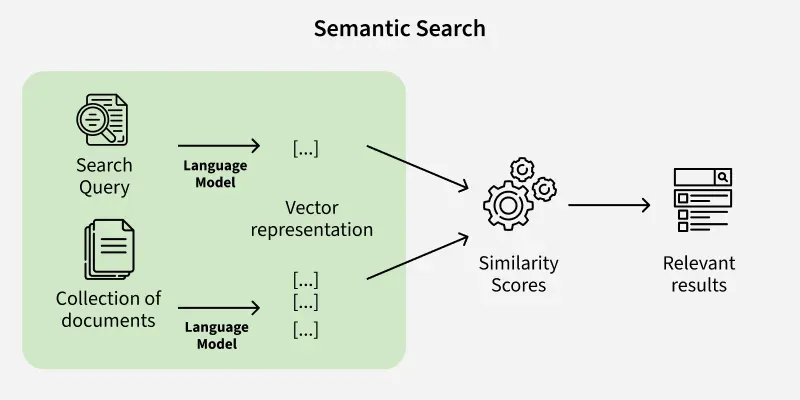
\includegraphics[width=0.75\textwidth]{Images/Kienthucnentang/Semantic-Search.png}
    \caption{Quy trình tìm kiếm ngữ nghĩa từ truy vấn đến kết quả xếp hạng \parencite{geeksforgeeks_semantic_search}}
    \label{fig:semantic_search_pipeline}
\end{figure}

Tìm kiếm đa phương thức mở rộng bài toán bằng cách tiếp nhận nhiều dạng dữ liệu. Trong phạm vi đồ án, hai modality chính là văn bản và hình ảnh. Người dùng có thể tải ảnh để tìm sản phẩm tương tự, hoặc kết hợp ảnh với mô tả như “tìm mẫu giống ảnh này nhưng màu đen”. Hệ thống khi đó phải khai thác cả đặc trưng thị giác, ngữ nghĩa văn bản và metadata sản phẩm trước khi tạo thứ hạng cuối cùng.

\begin{figure}[H]
    \centering
    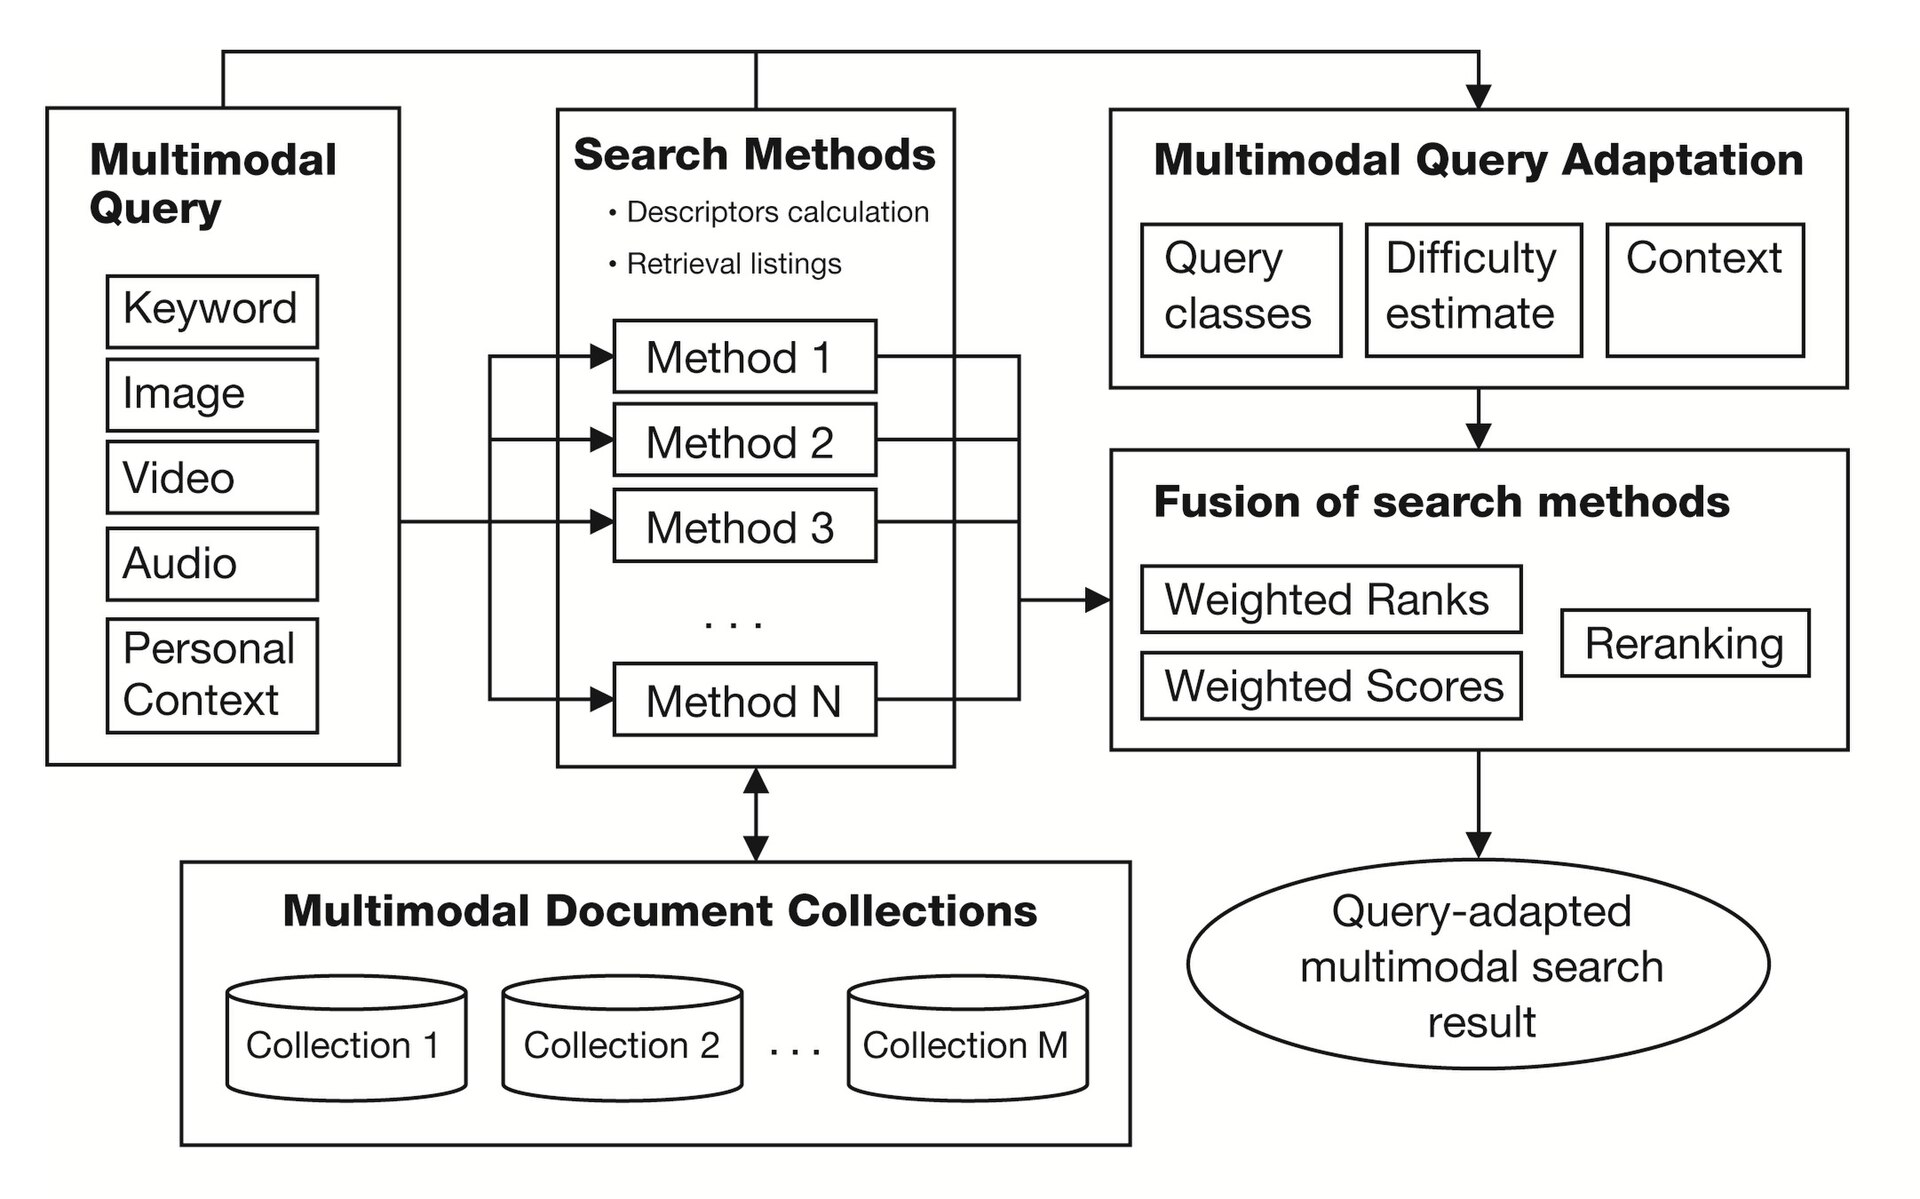
\includegraphics[width=0.72\textwidth]{Images/Kienthucnentang/Framework_of_Multimodal_Search.jpg}
    \caption{Khái quát hệ thống tìm kiếm kết hợp truy vấn văn bản và hình ảnh \parencite{ipullrank_mum_search}}
    \label{fig:multimodal_search_overview}
\end{figure}

\subsection{Biểu diễn embedding đa phương thức}

\subsubsection{Vector embedding và không gian ngữ nghĩa}

Vector embedding là phép ánh xạ một đối tượng như câu văn, hình ảnh hoặc sản phẩm thành vector số thực có số chiều cố định. Embedding được học từ dữ liệu để lưu giữ các đặc trưng có ích cho việc so sánh ngữ nghĩa \parencite{pinecone_embedding}. Tập các vector tạo thành không gian embedding, trong đó vị trí tương đối giữa các vector phản ánh mức độ liên quan theo cách mà mô hình đã học.

Trong đồ án, dữ liệu sản phẩm được embedding trước và lưu vào cơ sở dữ liệu vector. Khi tìm kiếm, truy vấn mới được đưa qua mô hình tương ứng để sinh vector, sau đó so sánh với các vector đã lập chỉ mục. Chất lượng embedding ảnh hưởng trực tiếp đến khả năng nhận biết từ đồng nghĩa, phong cách, loại sản phẩm và sự tương đồng thị giác.

\subsubsection{Embedding văn bản}

Text embedding chuyển câu truy vấn hoặc nội dung sản phẩm thành vector ngữ nghĩa. Nội dung biểu diễn sản phẩm có thể tổng hợp từ tên, mô tả, danh mục và các thuộc tính liên quan. Semantic retrieval sau đó tìm các sản phẩm có vector gần với vector truy vấn.

Embedding giúp giảm sự phụ thuộc vào đối sánh bề mặt. Chẳng hạn, “váy đi tiệc” và “đầm dự sự kiện” có thể được xem là gần nhau về nhu cầu sử dụng. Tuy vậy, embedding không thay thế hoàn toàn việc trích xuất điều kiện. Các ràng buộc chính xác như mức giá tối đa hoặc trạng thái còn bán cần được xử lý bằng metadata filtering.

\subsubsection{Embedding hình ảnh}

Image embedding chuyển hình ảnh thành vector đặc trưng biểu diễn các yếu tố thị giác như hình dạng, màu sắc, họa tiết, chất liệu biểu kiến và kiểu dáng. Khi người dùng tải ảnh, hệ thống sinh vector cho ảnh truy vấn rồi thực hiện tìm kiếm tương đồng trên các vector ảnh sản phẩm. Đây là nền tảng của image-to-product retrieval và visual search.

Ảnh đầu vào cần được chuẩn hóa về định dạng, kích thước và hướng ảnh trước khi sinh embedding. Nếu ảnh chứa nhiều vật thể hoặc phần nền lớn, một vùng quan tâm có thể được người dùng chọn hoặc được bộ phát hiện đối tượng đề xuất. Ảnh toàn phần vẫn là đầu vào dự phòng để tránh làm mất sản phẩm khi bước phát hiện không chắc chắn.

\subsubsection{Không gian embedding chung cho văn bản và hình ảnh}

Multimodal embedding ánh xạ văn bản và hình ảnh vào một không gian tương thích. Các mô hình thị giác--ngôn ngữ thường sử dụng hai encoder cho hai modality và huấn luyện theo mục tiêu tương phản để đưa các cặp văn bản--ảnh phù hợp lại gần nhau \parencite{clip_paper}. Nhờ đó, hệ thống có thể thực hiện text-to-image, image-to-image và truy hồi kết hợp.

\begin{figure}[H]
    \centering
    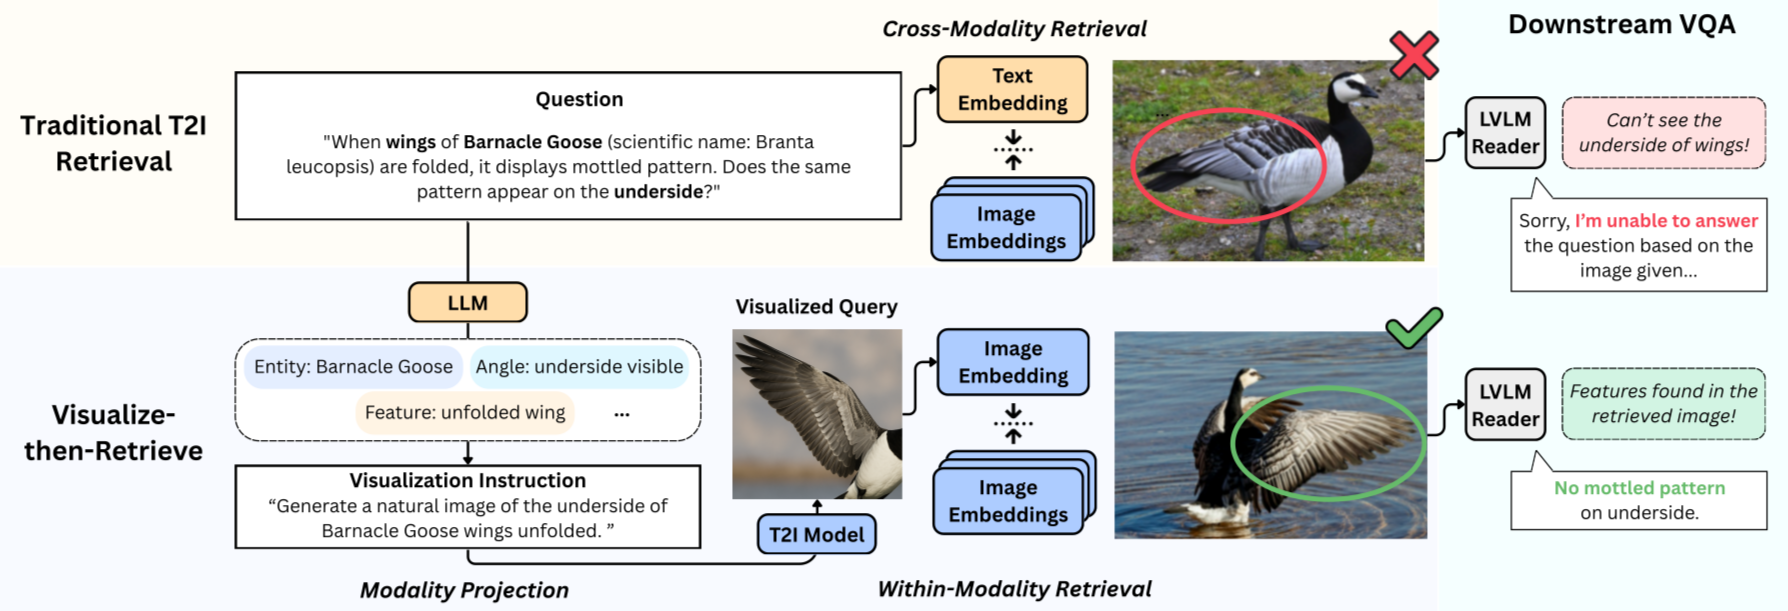
\includegraphics[width=0.78\textwidth]{Images/Kienthucnentang/text-image-retrieval.png}
    \caption{Ánh xạ văn bản và hình ảnh vào không gian biểu diễn chung để thực hiện truy hồi đa phương thức \parencite{faghri2018vsepp}}
    \label{fig:text_image_retrieval}
\end{figure}

Trong đồ án, văn bản và hình ảnh tạo thành hai nhánh truy hồi. Kết quả của mỗi nhánh được hợp nhất theo sản phẩm, sau đó kết hợp với mức khớp thuộc tính và tín hiệu nghiệp vụ. Cách tổ chức này cho phép hệ thống tận dụng không gian embedding chung nhưng vẫn kiểm soát riêng đóng góp của từng modality.

\subsection{Truy hồi vector}

\subsubsection{Cơ sở dữ liệu vector}

Cơ sở dữ liệu vector quản lý embedding cùng metadata và cung cấp phép tìm kiếm các vector gần nhất \parencite{wang2021milvus}. Mỗi điểm dữ liệu thường gồm định danh, vector và payload mô tả đối tượng. Trong bài toán sản phẩm, payload có thể chứa mã sản phẩm, danh mục, thương hiệu, màu, chất liệu, kích thước, giới tính, giá bán và trạng thái hoạt động.

Việc lưu vector cùng payload cho phép hệ thống kết hợp similarity search với điều kiện lọc. Ví dụ, sau khi biểu diễn ngữ nghĩa của “váy dự tiệc”, truy vấn vector có thể đồng thời giới hạn màu đỏ, giá không vượt quá một triệu đồng và chỉ lấy sản phẩm đang hoạt động.

\subsubsection{Độ tương đồng vector}

Độ tương đồng vector định lượng mức độ gần nhau giữa vector truy vấn và vector sản phẩm. Các phép đo phổ biến gồm cosine similarity, dot product và Euclidean distance. Cosine similarity đo góc giữa hai vector và thường được sử dụng khi hướng của vector quan trọng hơn độ lớn \parencite{qdrant2024vectorsimilarity}:

\begin{equation}
    \operatorname{cos}(\mathbf{q},\mathbf{x})=
    \frac{\mathbf{q}\cdot\mathbf{x}}
    {\lVert\mathbf{q}\rVert_2\lVert\mathbf{x}\rVert_2}.
    \label{eq:cosine_similarity}
\end{equation}

Trong đó, $\mathbf{q}$ là vector truy vấn và $\mathbf{x}$ là vector sản phẩm. Điểm tương đồng là tín hiệu quan trọng cho xếp hạng nhưng không phải tín hiệu duy nhất; hệ thống còn phải xét điều kiện lọc, mức khớp thuộc tính và các tín hiệu nghiệp vụ.

\begin{figure}[H]
    \centering
    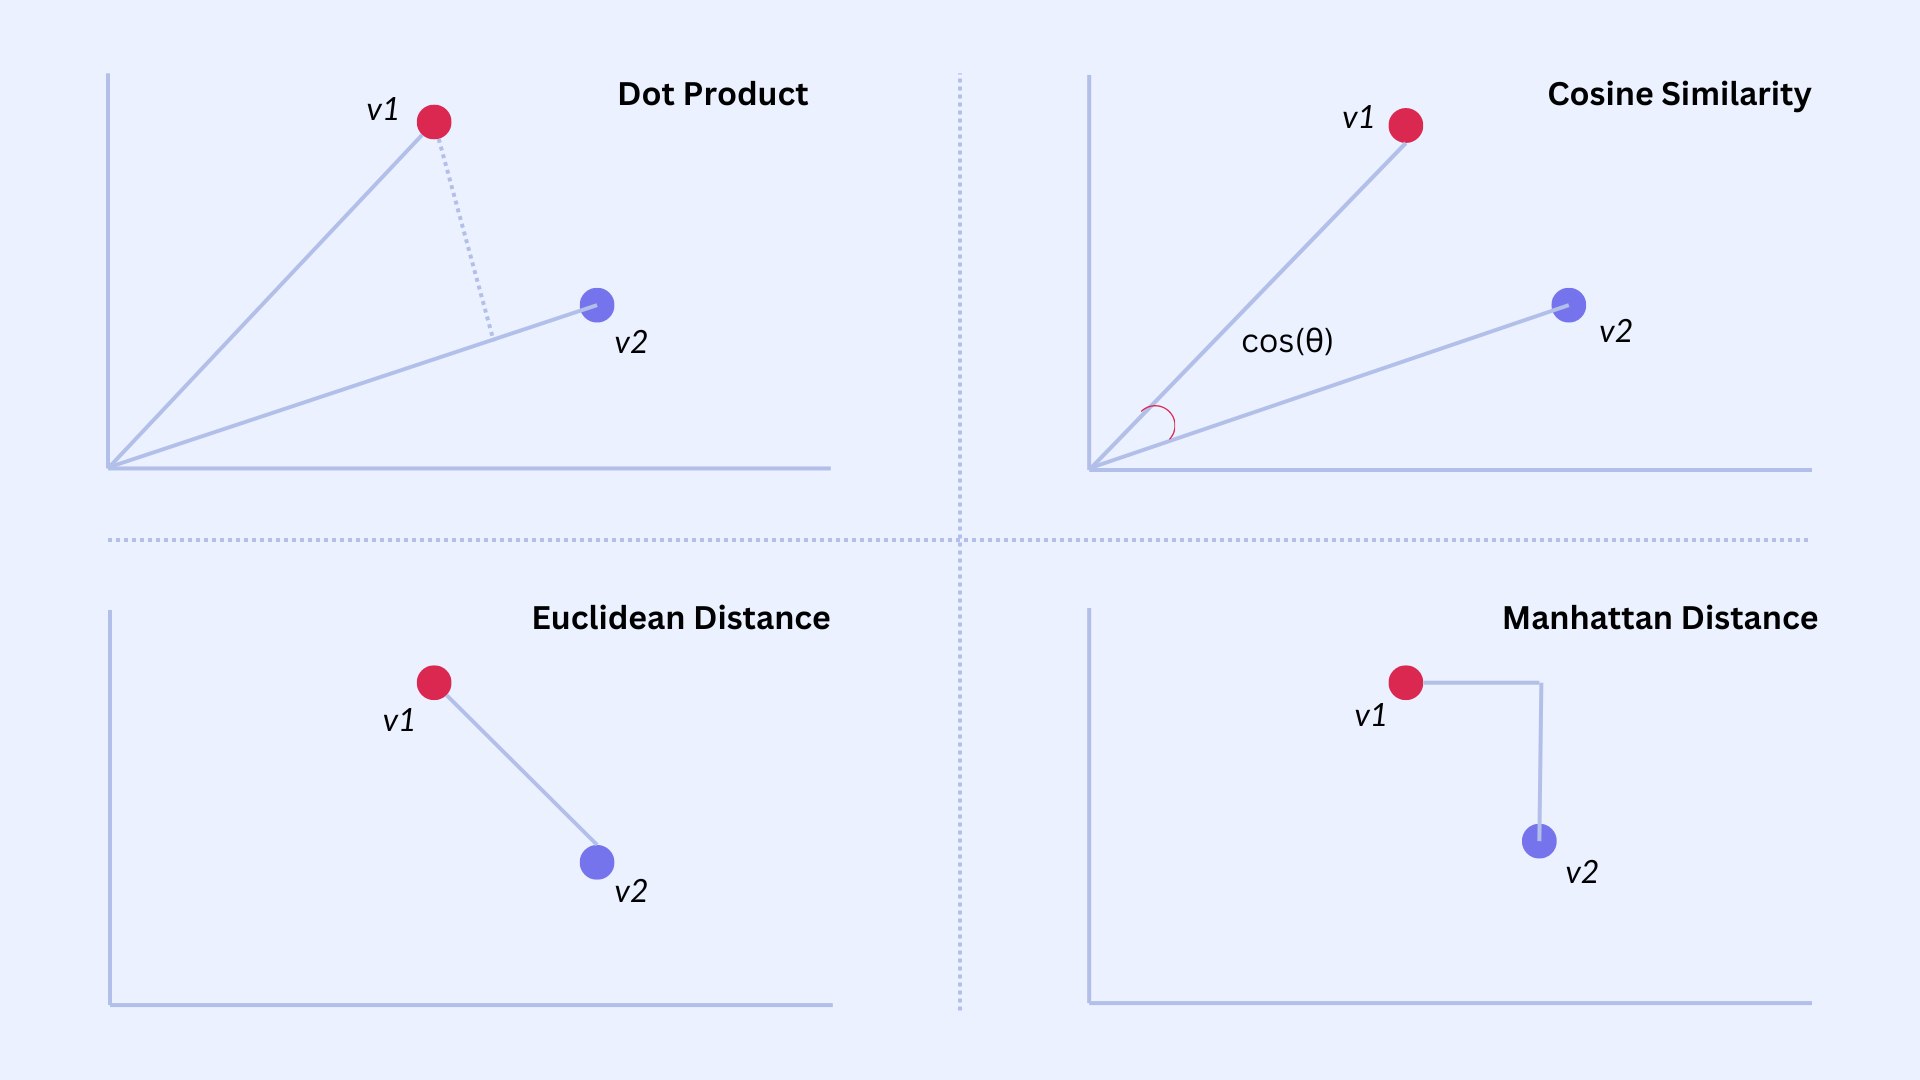
\includegraphics[width=0.72\linewidth]{Images/Kienthucnentang/vector-similarity.png}
    \caption{Các vector có nội dung tương tự được phân bố gần nhau trong không gian embedding \parencite{qdrant2024vectorsimilarity}}
    \label{fig:vector_similarity}
\end{figure}

\subsubsection{Approximate Nearest Neighbor và HNSW}

Với số lượng vector lớn, so sánh truy vấn với mọi vector có chi phí tuyến tính theo kích thước dữ liệu. Approximate Nearest Neighbor (ANN) giảm chi phí bằng cách tìm tập lân cận gần đúng thay vì bảo đảm duyệt toàn bộ không gian \parencite{arya1998optimal}. Sự đánh đổi này phù hợp với hệ thống tìm kiếm tương tác vì giảm độ trễ trong khi vẫn duy trì chất lượng truy hồi ở mức cao.

Hierarchical Navigable Small World (HNSW) là một phương pháp ANN dựa trên đồ thị nhiều tầng \parencite{malkov2018efficient}. Các tầng trên chứa liên kết thưa để di chuyển nhanh giữa các vùng xa, còn tầng thấp chứa liên kết dày hơn để tinh chỉnh lân cận.

\begin{figure}[H]
    \centering
    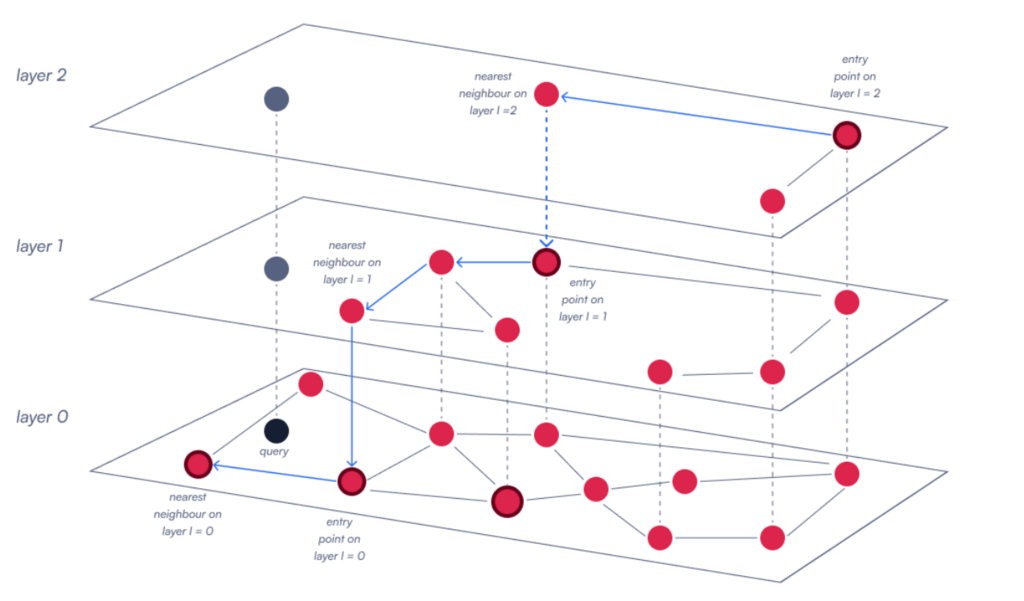
\includegraphics[width=0.72\linewidth]{Images/Kienthucnentang/hnsw-overview.png}
    \caption{Cấu trúc đồ thị nhiều tầng của HNSW trong tìm kiếm lân cận gần đúng \parencite{qdrant2024hnsw}}
    \label{fig:hnsw_overview}
\end{figure}

\subsection{Hiểu và xử lý truy vấn sản phẩm}

\subsubsection{Phân tích ý định và trích xuất thuộc tính}

Query understanding là quá trình xác định mục đích và các thông tin có cấu trúc trong phát biểu của người dùng \parencite{guo2020deep}. Đối với trợ lý mua sắm, các ý định quan trọng gồm tìm kiếm bằng văn bản, tìm kiếm bằng ảnh, tìm kiếm kết hợp, hỏi thông tin sản phẩm, so sánh, làm rõ yêu cầu và tiếp tục hội thoại.

Sau khi nhận diện ý định, hệ thống trích xuất các thuộc tính như danh mục, thương hiệu, màu sắc, chất liệu, kích thước, giới tính, mục đích sử dụng và khoảng giá. Kết quả phân tích có cấu trúc để các bước phía sau có thể kiểm tra, chuẩn hóa và áp dụng nhất quán. Cách tiếp cận kết hợp luật xác định với LLM giúp xử lý nhanh các mẫu rõ ràng, đồng thời hỗ trợ truy vấn tự nhiên và phụ thuộc ngữ cảnh.

\subsubsection{Chuẩn hóa, ánh xạ bí danh và viết lại truy vấn}

Ngôn ngữ tìm kiếm sản phẩm có nhiều biến thể: có dấu hoặc không dấu, tên tiếng Việt hoặc tiếng Anh, cách viết tắt, lỗi gõ và tên gọi không thống nhất. Chuẩn hóa truy vấn đưa các biểu diễn này về dạng nhất quán; ánh xạ bí danh liên kết các cách gọi tương đương với danh mục và thuộc tính chuẩn của hệ thống.

Query rewrite tạo một biểu diễn phù hợp hơn cho bước embedding và retrieval nhưng phải bảo toàn ý định ban đầu \parencite{ren2010query}. Với hội thoại nhiều lượt, truy vấn viết lại có thể bổ sung ngữ cảnh còn hiệu lực. Sau yêu cầu “tìm váy dự tiệc màu đỏ”, câu “loại dưới 800 nghìn” có thể được diễn giải thành truy vấn đầy đủ chứa cả loại sản phẩm, mục đích, màu sắc và giới hạn giá mới.

Việc viết lại không được tự tạo thêm ràng buộc mà người dùng chưa yêu cầu. Giá trị do câu chữ hiện tại nêu rõ có độ tin cậy cao hơn thuộc tính chỉ được suy ra từ mô hình. Nguyên tắc này giúp hạn chế việc loại bỏ sản phẩm phù hợp do diễn giải quá mức.

\subsubsection{Ràng buộc cứng, ràng buộc mềm và metadata filtering}

Metadata filtering áp dụng điều kiện có cấu trúc lên tập ứng viên. Một số điều kiện mang tính bắt buộc, chẳng hạn giá tối đa, thương hiệu được nêu trực tiếp hoặc trạng thái sản phẩm đang bán. Những điều kiện này được xem là ràng buộc cứng và có thể dùng để loại sản phẩm không thỏa mãn.

Ngược lại, thuộc tính chỉ được suy ra hoặc có tính chủ quan như phong cách, dịp sử dụng và một số sắc độ màu nên được xem là ràng buộc mềm. Thay vì loại bỏ ứng viên, hệ thống có thể cộng điểm cho sản phẩm phù hợp. Khi ràng buộc suy diễn làm tập kết quả quá hẹp, cơ chế recovery có thể nới điều kiện mềm nhưng vẫn giữ nguyên các yêu cầu rõ ràng của người dùng.

Việc phân biệt nguồn gốc ràng buộc giúp cân bằng precision và recall. Hard filter cải thiện tính tuân thủ đối với yêu cầu chính xác, còn soft boost giảm nguy cơ bỏ sót do metadata chưa đầy đủ hoặc mô hình hiểu truy vấn chưa chắc chắn.

\subsection{Tìm kiếm đa phương thức và xếp hạng}

\subsubsection{Truy hồi bằng văn bản và hình ảnh}

Nhánh văn bản sinh embedding cho truy vấn đã được chuẩn hóa, truy hồi trên tập vector văn bản và kết hợp các kết quả khớp tên chính xác. Nhánh hình ảnh chuẩn hóa ảnh đầu vào, sinh image embedding và truy hồi trên tập vector ảnh. Do một sản phẩm có thể có nhiều ảnh, kết quả ảnh cần được quy về mức sản phẩm và loại bỏ định danh trùng lặp trước khi trả về.

Đối với ảnh có nhiều đối tượng, Object Detection có thể hỗ trợ xác định bounding box và crop vùng chứa sản phẩm \parencite{redmon2016yolo}. Kết quả phát hiện thường gồm nhãn, tọa độ và confidence score. Trong phạm vi đồ án, đây là bước tăng cường tùy chọn; ảnh toàn phần vẫn được sử dụng khi bộ phát hiện bị tắt hoặc không tìm được vùng đủ tin cậy.

\subsubsection{Hybrid multimodal retrieval}

Khi truy vấn đồng thời có văn bản và hình ảnh, hai nhánh retrieval có thể chạy độc lập rồi hợp nhất theo mã sản phẩm. Một sản phẩm có thể xuất hiện ở một hoặc cả hai nhánh. Cách tiếp cận này giữ được thông tin riêng của từng modality và cho phép quan sát đóng góp của văn bản so với hình ảnh.

Ví dụ, với ảnh một chiếc váy và yêu cầu “mẫu tương tự nhưng màu đen, dưới một triệu”, nhánh ảnh tập trung vào kiểu dáng và đặc trưng thị giác; nhánh văn bản biểu diễn phần mô tả; metadata filtering kiểm soát màu và giá. Kết quả cuối cần thỏa mãn ràng buộc rõ ràng, đồng thời vẫn gần ảnh tham chiếu.

\subsubsection{Weighted fusion và reranking}

Fusion kết hợp nhiều tín hiệu thành điểm xếp hạng chung. Với sản phẩm $p$, điểm có thể được biểu diễn tổng quát như sau:

\begin{equation}
    S(p)=w_iS_i(p)+w_tS_t(p)+w_fS_f(p)+w_bS_b(p)+S_u(p),
    \label{eq:multimodal_fusion}
\end{equation}

trong đó $S_i$ và $S_t$ lần lượt là độ tương đồng ảnh và văn bản; $S_f$ là mức khớp ràng buộc mềm; $S_b$ là tín hiệu nghiệp vụ; $S_u$ là phần tăng cường theo mục đích sử dụng; các hệ số $w$ kiểm soát đóng góp của từng tín hiệu. Các điểm số cần được đưa về thang đo tương thích trước khi cộng có trọng số.

Sau bước truy hồi ban đầu, reranking đánh giá lại một tập ứng viên nhỏ để cải thiện thứ tự kết quả \parencite{reranking_sbert}. Vì reranking tăng chi phí và độ trễ, nó chỉ nên áp dụng lên top-$k$ ứng viên và được bật khi thử nghiệm chứng minh lợi ích về chất lượng.

\subsection{Large Language Model và Retrieval-Augmented Generation}

\subsubsection{Vai trò của Large Language Model}

Large Language Model (LLM) là mô hình học sâu có khả năng hiểu và sinh ngôn ngữ tự nhiên, thường dựa trên kiến trúc Transformer và cơ chế self-attention \parencite{vaswani2017attention}. Trong trợ lý mua sắm, LLM hỗ trợ phân loại ý định, trích xuất thuộc tính, viết lại truy vấn theo ngữ cảnh và tạo phản hồi hội thoại.

LLM không nên tự suy đoán giá, tồn kho hoặc thuộc tính sản phẩm. Những dữ kiện này thay đổi theo dữ liệu nghiệp vụ và cần được lấy từ các dịch vụ của hệ thống. Vai trò phù hợp của LLM là diễn giải nhu cầu và tổng hợp thông tin đã được truy hồi thành câu trả lời dễ hiểu.

\subsubsection{Prompt và đầu ra có cấu trúc}

Prompt là tập hướng dẫn và ngữ cảnh được cung cấp cho LLM. Một prompt cho trợ lý mua sắm thường gồm vai trò của hệ thống, yêu cầu của người dùng, lịch sử hội thoại liên quan, các ràng buộc an toàn, dữ liệu sản phẩm đã truy hồi và định dạng đầu ra mong muốn.

Ở bước hiểu truy vấn, đầu ra có cấu trúc giúp kiểm tra các trường như intent, rewritten query, category, color và price range trước khi truy hồi. Ở bước sinh câu trả lời, prompt cần yêu cầu mô hình chỉ sử dụng dữ kiện được cung cấp, không khẳng định trạng thái tồn kho hoặc thuộc tính không có trong context. Việc tách prompt phân tích khỏi prompt trả lời làm giảm sự phụ thuộc giữa điều phối nghiệp vụ và cách diễn đạt ngôn ngữ.

\subsubsection{Kiến trúc product-grounded RAG}

Retrieval-Augmented Generation kết hợp một thành phần truy hồi với một mô hình sinh để tạo phản hồi dựa trên dữ liệu bên ngoài \parencite{lewis2020rag}. Trong RAG tổng quát, retriever tìm các tài liệu liên quan và generator sử dụng chúng làm context. Đối với đồ án, đơn vị được truy hồi là sản phẩm thay vì đoạn văn thuần túy, vì vậy có thể xem đây là kiến trúc product-grounded RAG.

\begin{figure}[H]
    \centering
    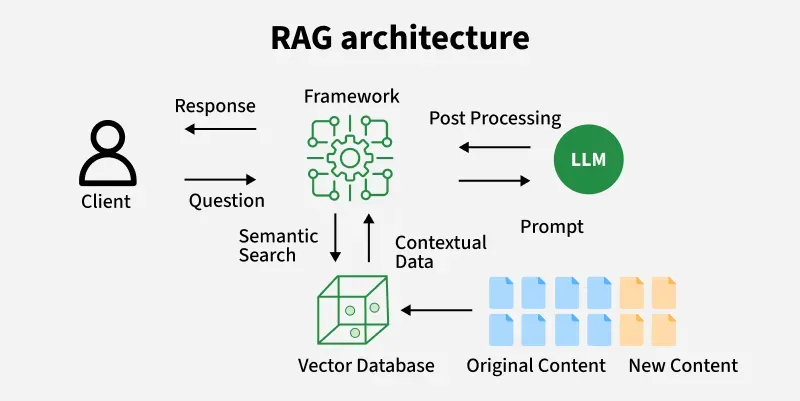
\includegraphics[width=0.75\textwidth]{Images/Kienthucnentang/RAG-architecture.png}
    \caption{Kiến trúc RAG kết hợp truy hồi dữ liệu và sinh phản hồi \parencite{geeksforgeeks2026ragarchitecture}}
    \label{fig:rag_architecture}
\end{figure}

Quy trình product-grounded RAG của trợ lý mua sắm gồm các bước chính:

\begin{enumerate}
    \item Phân tích ý định, truy vấn và các ràng buộc của người dùng.
    \item Truy hồi ứng viên bằng nhánh văn bản, hình ảnh hoặc hybrid.
    \item Lấy metadata và trạng thái kinh doanh hiện hành của các sản phẩm ứng viên.
    \item Xây dựng context có cấu trúc từ các dữ kiện đã xác minh.
    \item Yêu cầu LLM tổng hợp câu trả lời và giải thích gợi ý dựa trên context.
\end{enumerate}

Kiến trúc này giúp giảm hallucination và làm cho phản hồi có căn cứ hơn. Tuy nhiên, RAG không tự bảo đảm tính đúng đắn: chất lượng cuối cùng còn phụ thuộc vào recall của retriever, tính mới của dữ liệu nghiệp vụ, cách xây dựng context và mức độ tuân thủ prompt của generator.

\subsubsection{Bộ nhớ hội thoại}

Conversation memory duy trì thông tin cần thiết giữa các lượt trao đổi. Bộ nhớ có thể chứa tiêu chí đang áp dụng, giá trị đã bị thay thế, sản phẩm người dùng vừa tham chiếu, quyết định đã xác nhận và câu hỏi còn chưa được làm rõ. Nhờ đó, trợ lý có thể xử lý những phát biểu rút gọn như “mẫu thứ hai”, “đổi sang màu đen” hoặc “rẻ hơn một chút”.

Bộ nhớ hội thoại có thể kết hợp lịch sử gần nhất, bản tóm tắt hội thoại và trạng thái có cấu trúc. Lịch sử giữ nguyên cách diễn đạt gần đây; bản tóm tắt giới hạn kích thước context; trạng thái có cấu trúc giúp truy cập chính xác các ràng buộc đang có hiệu lực. Dữ liệu cần được phân tách theo người dùng và phiên hội thoại, đồng thời có chính sách giới hạn dung lượng và thời gian lưu trữ.

\subsection{Đánh giá chất lượng hệ thống}

\subsubsection{Các chỉ số đánh giá truy hồi}

Đánh giá retrieval cần xem xét cả khả năng tìm đúng sản phẩm và chất lượng thứ hạng. Với tập kết quả top-$k$, các chỉ số phù hợp gồm:

\begin{itemize}
    \item \textbf{Hit@$k$}: cho biết ít nhất một sản phẩm liên quan có xuất hiện trong top-$k$ hay không.
    \item \textbf{Precision@$k$}: tỷ lệ sản phẩm liên quan trong $k$ kết quả đầu.
    \item \textbf{Recall@$k$}: tỷ lệ sản phẩm liên quan đã được tìm thấy trong top-$k$ so với toàn bộ tập liên quan.
    \item \textbf{MRR}: trung bình nghịch đảo thứ hạng của kết quả đúng đầu tiên.
    \item \textbf{nDCG@$k$}: đánh giá thứ hạng khi sản phẩm có nhiều mức độ liên quan khác nhau và giảm trọng số ở các vị trí thấp.
\end{itemize}

Các chỉ số cần được diễn giải theo cách xây dựng ground truth. Ví dụ, Recall@$k$ không phản ánh đầy đủ khả năng bao phủ toàn danh mục nếu tập nhãn chỉ được tạo từ chính các ứng viên của một lần chạy. Đối với tìm kiếm ảnh, cần phân biệt truy hồi đúng sản phẩm gốc với truy hồi các sản phẩm tương tự về mặt thị giác.

\subsubsection{Grounding và chất lượng phản hồi}

Đối với RAG, tìm đúng sản phẩm chưa đủ; câu trả lời còn phải sử dụng đúng dữ kiện trong context. Grounding đo mức độ các khẳng định về tên, giá, màu, chất liệu hoặc tình trạng bán được hỗ trợ bởi dữ liệu đã truy hồi. Response relevancy đánh giá câu trả lời có trực tiếp giải quyết yêu cầu của người dùng hay không. Các tình huống so sánh, truy vấn tiếp nối và thay đổi tiêu chí cần được đánh giá theo hội thoại nhiều lượt.

\subsubsection{Độ trễ xử lý}

Độ trễ ảnh hưởng trực tiếp đến trải nghiệm hội thoại. Ngoài thời gian end-to-end, nên đo riêng thời gian hiểu truy vấn, sinh embedding, truy vấn cơ sở dữ liệu vector, reranking, lấy dữ liệu nghiệp vụ và sinh phản hồi. Các phân vị p50 và p95 phản ánh độ ổn định tốt hơn so với chỉ sử dụng giá trị trung bình. Việc đánh giá chất lượng và độ trễ đồng thời giúp lựa chọn cấu hình candidate pool và reranker phù hợp.

\subsection*{Kết chương}

Chương này đã trình bày các nền tảng trực tiếp của trợ lý mua sắm đa phương thức: tìm kiếm ngữ nghĩa, embedding văn bản--hình ảnh, truy hồi vector, hiểu truy vấn, metadata filtering, hybrid fusion và reranking. Những thành phần này cho phép hệ thống xử lý các yêu cầu tự nhiên có nhiều thuộc tính cũng như truy vấn bằng ảnh hoặc kết hợp hai modality.

Bên cạnh retrieval, chương đã trình bày vai trò của LLM, product-grounded RAG và bộ nhớ hội thoại trong việc tạo phản hồi có căn cứ và duy trì ngữ cảnh nhiều lượt. Cuối cùng, các chỉ số retrieval, grounding và độ trễ cung cấp cơ sở để đánh giá toàn diện chất lượng của hệ thống ở các chương sau.

\section{Công nghệ và quyết định lựa chọn}

Chương này trình bày các công nghệ được sử dụng trong hệ thống và lý do lựa chọn chúng. Nội dung được tổ chức theo luồng xử lý từ giao diện, Backend nghiệp vụ, AI Service, xử lý đa phương thức, truy hồi đến hạ tầng triển khai. Các nguyên lý lý thuyết đã được trình bày ở Chương 2; kiến trúc chi tiết và quy trình cài đặt lần lượt thuộc Chương 7 và Chương 8 nên không lặp lại tại đây.

\subsection{Tiêu chí và tổng quan lựa chọn công nghệ}

Các công nghệ được lựa chọn theo năm tiêu chí chính:

\begin{itemize}
    \item đáp ứng các chức năng thương mại điện tử, tìm kiếm đa phương thức và hội thoại RAG;
    \item phù hợp với dữ liệu, mã nguồn và năng lực triển khai của đề tài;
    \item có hợp đồng giao tiếp rõ ràng, thuận tiện kiểm thử và thay thế thành phần;
    \item vận hành được bằng container trong cả môi trường cục bộ và Google Cloud;
    \item cân bằng chất lượng, độ trễ, chi phí và yêu cầu quản trị hạ tầng.
\end{itemize}

Theo các tiêu chí trên, hệ thống sử dụng React ở lớp giao diện, Spring Boot và MySQL ở lớp nghiệp vụ, FastAPI và LangGraph ở AI Service, Cohere Embed v4 cùng Qdrant cho truy hồi đa phương thức, và Docker--Google Cloud cho triển khai. Redis được dùng cho trạng thái hội thoại ở môi trường Cloud Run. YOLOv26 hỗ trợ phát hiện vùng sản phẩm trong môi trường có cài mô hình cục bộ; cấu hình Cloud Run sử dụng ảnh đầy đủ để tránh phụ thuộc GPU và thư viện thị giác nặng.

\subsection{Công nghệ xây dựng giao diện}

\subsubsection{React}

Frontend sử dụng React 19 để xây dựng giao diện theo component \parencite{reactdocs2024}. Mô hình này phù hợp với các màn hình có nhiều trạng thái tương tác như bộ lọc, danh sách kết quả, thẻ sản phẩm, giỏ hàng, vùng tải ảnh và hội thoại nhiều lượt. Các component có thể tái sử dụng giữa tìm kiếm văn bản, hình ảnh và kết hợp mà không phải nhân bản toàn bộ giao diện.

React được chọn thay vì một framework full-stack vì Frontend của hệ thống chỉ giao tiếp với Spring Boot qua REST API, không đảm nhiệm nghiệp vụ hoặc truy cập trực tiếp dữ liệu. Hạn chế chính là trạng thái có thể trở nên phức tạp khi nhiều request cập nhật đồng thời; do đó trạng thái tìm kiếm, hội thoại và nghiệp vụ được tách theo từng nhóm chức năng.

\subsubsection{Redux Toolkit, React Router và Axios}

Redux Toolkit quản lý các trạng thái dùng chung như phiên đăng nhập, giỏ hàng và dữ liệu cần chia sẻ giữa nhiều màn hình. React Router tổ chức điều hướng phía client; Axios đảm nhiệm lời gọi HTTP và cho phép xử lý tập trung token, timeout cùng lỗi API. Bootstrap và SCSS cung cấp hệ thống bố cục responsive, còn Vite đảm nhiệm dev server và quá trình build.

Nhóm thư viện này được lựa chọn vì phù hợp với ứng dụng React dạng single-page application và giảm lượng mã nền phải tự xây dựng. Các thư viện chỉ xử lý trình bày và giao tiếp; mọi quyết định về quyền truy cập, giá, tồn kho và trạng thái đơn hàng vẫn do Backend xác nhận.

\subsection{Công nghệ Backend và dữ liệu nghiệp vụ}

\subsubsection{Java và Spring Boot}

Backend sử dụng Java 21 và Spring Boot 4.0.6. Spring Boot cung cấp auto-configuration, embedded server và hệ sinh thái xây dựng REST API \parencite{springbootdocs2024}. Công nghệ này phù hợp với nghiệp vụ thương mại điện tử có nhiều ràng buộc giao dịch như giỏ hàng, tồn kho, khuyến mãi, đơn hàng và thanh toán COD.

Spring Boot được chọn vì hỗ trợ transaction, validation, security và truy cập dữ liệu quan hệ đồng bộ trong một nền tảng thống nhất. So với một API Python tối giản, ứng dụng Java có thời gian khởi động và cấu hình lớn hơn; vì vậy phần suy luận AI được tách sang FastAPI thay vì đưa vào cùng tiến trình Backend.

\subsubsection{Spring Security, JPA và RestClient}

Spring Web MVC được dùng cho controller và REST endpoint; Spring Data JPA ánh xạ entity và truy cập MySQL; Spring Security cùng OAuth2 Client xử lý xác thực và phân quyền. RestClient thực hiện giao tiếp nội bộ với AI Service, còn Spring AOP và AspectJ hỗ trợ các tác vụ cắt ngang như ghi log hoặc kích hoạt đồng bộ catalog.

Việc sử dụng các module trong cùng hệ sinh thái giúp chính sách transaction, validation và lỗi API nhất quán. Backend đồng thời là cổng giao tiếp duy nhất của Frontend, nhờ đó khóa dịch vụ AI, Qdrant và cơ sở dữ liệu không bị đưa ra phía trình duyệt.

\subsubsection{MySQL}

MySQL 8.4 lưu dữ liệu nghiệp vụ gồm tài khoản, phân quyền, danh mục, sản phẩm, biến thể, giá, tồn kho, giỏ hàng, khuyến mãi và đơn hàng. MySQL được chọn vì mô hình quan hệ phù hợp với các ràng buộc khóa ngoại và giao dịch cần thiết cho thương mại điện tử, đồng thời được hỗ trợ trực tiếp bởi Spring Data JPA.

Trong hệ thống, MySQL là nguồn dữ liệu chuẩn. Qdrant chỉ đóng vai trò chỉ mục có thể tái tạo; kết quả AI chỉ chứa mã sản phẩm và điểm số, sau đó Backend đọc lại giá, tồn kho cùng trạng thái hiện hành từ MySQL trước khi trả cho người dùng.

\subsection{Công nghệ xây dựng AI Service}

\subsubsection{Python, FastAPI và Pydantic}

AI Service sử dụng Python 3.11 và FastAPI. FastAPI hỗ trợ API theo chuẩn ASGI, xử lý bất đồng bộ và sinh OpenAPI từ type hints \parencite{fastapidocs2024}. Pydantic xác thực, chuẩn hóa request/response; HTTPX thực hiện lời gọi tới Spring Boot và các dịch vụ mô hình; Pillow giải mã, resize và crop ảnh.

FastAPI được chọn vì hệ sinh thái Python thuận lợi cho embedding, xử lý ảnh và điều phối mô hình. Ranh giới REST giúp thay đổi provider embedding, LLM hoặc reranker mà không làm thay đổi giao diện người dùng. Đổi lại, hợp đồng giữa Backend và AI Service phải được kiểm soát phiên bản, timeout và lỗi fallback rõ ràng.

\subsubsection{LangGraph và Redis}

LangGraph điều phối workflow hội thoại có trạng thái dưới dạng graph \parencite{langgraph2024docs}. Các node thực hiện tải ngữ cảnh, hiểu truy vấn, định tuyến, truy hồi, lấy dữ liệu sản phẩm và sinh phản hồi; conditional edge quyết định nhánh xử lý theo ý định cùng dữ liệu đầu vào. LangGraph phù hợp hơn một chain tuyến tính vì trợ lý cần clarification, memory recall và nhiều đường đi có kiểm soát.

Ở môi trường Cloud Run, Redis lưu checkpoint và preference memory có thời hạn. Redis hỗ trợ truy cập nhanh và chia sẻ trạng thái ngoài tiến trình, phù hợp khi container AI Service có thể được thay thế. SQLite chỉ dùng cho phát triển hoặc kiểm thử đơn instance. Hệ thống không xem workflow này là agent tự trị: các node, công cụ và điều kiện chuyển trạng thái đều được giới hạn trước.

\subsubsection{LLM qua Amazon Bedrock}

Cấu hình triển khai sử dụng mô hình ngôn ngữ được quản lý qua Amazon Bedrock. LLM đảm nhiệm phân tích ý định, trích xuất thuộc tính, viết lại truy vấn và diễn đạt câu trả lời; dữ kiện về sản phẩm được cung cấp bởi tầng truy hồi và Backend thay vì lấy từ tri thức tham số của mô hình.

Dịch vụ managed giúp không phải vận hành GPU cho LLM và cho phép thay model qua cấu hình. Hạn chế là phụ thuộc vào mạng, quota, chi phí và chính sách provider; vì vậy AI Service áp dụng timeout, retry có giới hạn, fallback và ghi nhận model cùng độ trễ cho từng lần gọi.

\subsection{Công nghệ xử lý ảnh và embedding đa phương thức}

\subsubsection{YOLOv26 và Pillow}

YOLO được lựa chọn cho bước phát hiện vùng chứa sản phẩm nhờ kiến trúc one-stage và khả năng suy luận nhanh \parencite{redmon2016yolo}. Trong đồ án, YOLOv26s được fine-tune trên dữ liệu thời trang để nhận diện bốn nhóm tổng quát gồm phụ kiện, túi, quần áo và giày. Bounding box có độ tin cậy phù hợp được dùng để crop sản phẩm trước khi tạo image embedding; Pillow thực hiện các thao tác giải mã và chuẩn hóa ảnh.

YOLO là bước tăng cường, không phải điều kiện bắt buộc của Image Search. Khi không phát hiện được vùng đủ tin cậy, hệ thống sử dụng ảnh đầy đủ. Mô hình được sử dụng trong môi trường cục bộ có cài Ultralytics; image Cloud Run dạng managed-only tắt YOLO và luôn dùng ảnh đầy đủ để giảm kích thước container cùng yêu cầu tài nguyên.

\subsubsection{Cohere Embed v4 qua Amazon Bedrock}

Cấu hình được đánh giá sử dụng \texttt{cohere.embed-v4:0} qua Amazon Bedrock để tạo vector 1.536 chiều cho cả văn bản và hình ảnh. Nhánh văn bản biểu diễn truy vấn và mô tả sản phẩm; nhánh hình ảnh biểu diễn ảnh catalog và ảnh do người dùng cung cấp. Hai loại vector được lưu ở hai collection riêng để tránh trộn modality và thuận tiện đánh giá độc lập.

Multimodal embedding managed giúp thống nhất không gian biểu diễn mà không phải phục vụ các mô hình vision--language cục bộ. Đổi lại, hệ thống chịu độ trễ mạng, quota và chi phí theo request. PyTorch, Transformers, Sentence-Transformers và OpenCLIP chỉ thuộc cấu hình \texttt{local-models} tùy chọn, không phải pipeline production được dùng trong đánh giá cuối.

\subsection{Công nghệ truy hồi và xếp hạng}

\subsubsection{Qdrant}

Qdrant lưu text/image embedding, mã sản phẩm và metadata phục vụ lọc \parencite{qdrant_docs}. Hệ thống duy trì collection riêng cho từng modality; mỗi point liên kết với \texttt{product\_id} và có thể mang các thuộc tính như danh mục, màu, chất liệu, giới tính, giá hoặc trạng thái hoạt động.

\begin{figure}[H]
    \centering
    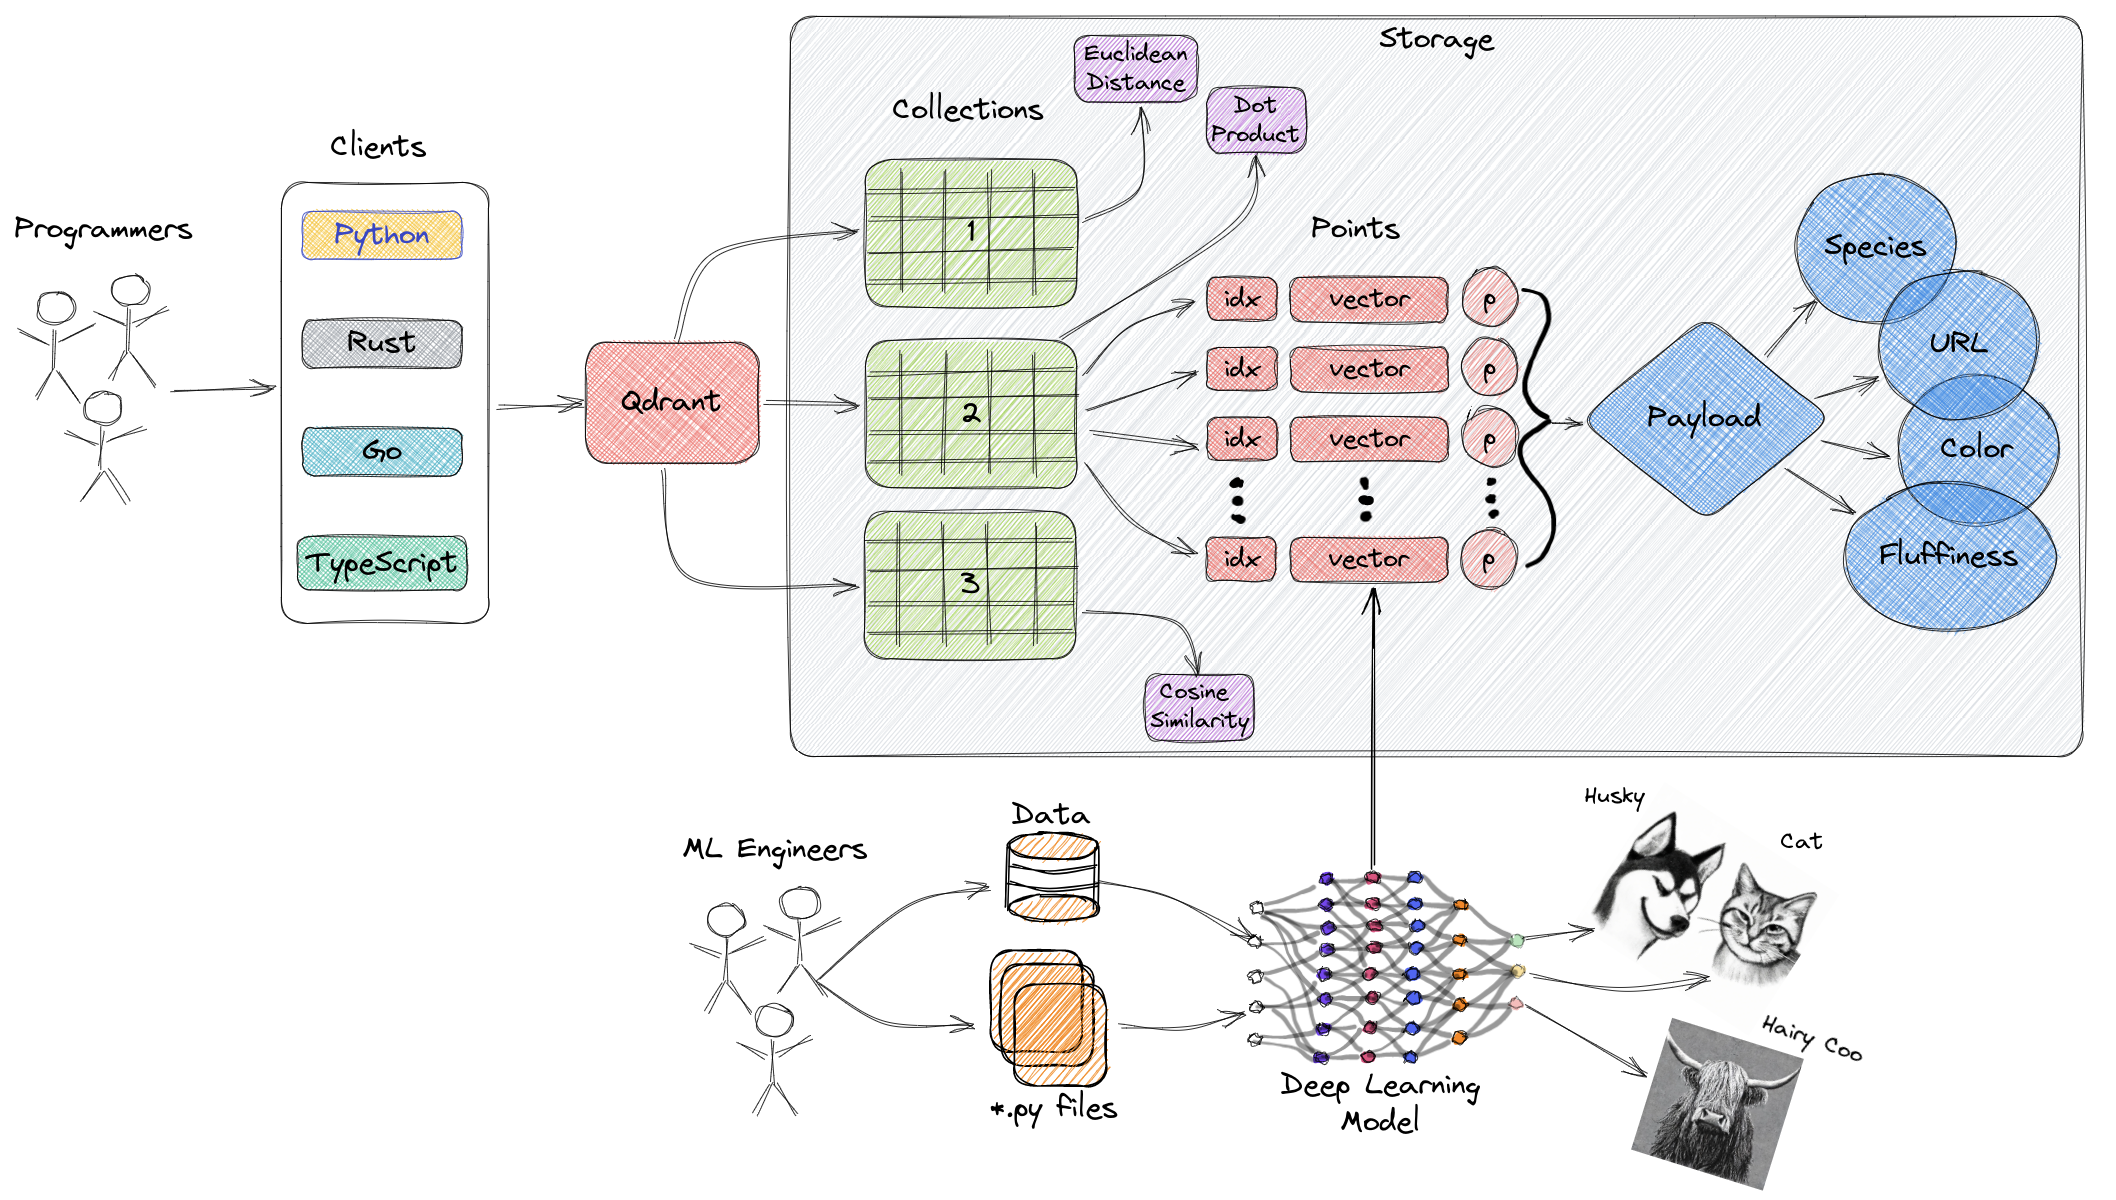
\includegraphics[width=0.86\linewidth]{Images/Congnghelienquan/qdrant_overview_high_level.png}
    \caption{Qdrant kết hợp vector engine, payload và filtering cho truy hồi sản phẩm \parencite{qdrant_overview}}
    \label{fig:selected_qdrant_architecture}
\end{figure}

Qdrant được chọn vì có thể self-host bằng Docker, hỗ trợ độ tương đồng cosine, truy hồi gần đúng bằng HNSW, lọc payload và API Python. So với dịch vụ vector được quản lý hoàn toàn, Qdrant cho phép kiểm soát dữ liệu và chi phí ở quy mô catalog hiện tại; hạn chế là nhóm phát triển phải tự quản lý volume, snapshot, backup và giám sát collection.

\subsubsection{Hybrid fusion và reranker}

Search Service truy hồi ứng viên độc lập từ nhánh văn bản và hình ảnh, quy về \texttt{product\_id}, sau đó hợp nhất điểm với metadata cùng ràng buộc nghiệp vụ. Cách tách first-stage retrieval và fusion giúp điều chỉnh trọng số giữa mức tương đồng ảnh với mức phù hợp văn bản mà không thay đổi vector database.

Google Cloud Ranking API được tích hợp như một reranker managed và chỉ hoạt động khi feature flag được bật. Đây là thành phần xếp hạng tùy chọn, không phải điều kiện của pipeline. Kết quả đánh giá ở Chương 9 cho thấy rerank hiện tại không cải thiện các chỉ số chính, vì vậy cấu hình được lựa chọn để báo cáo là fusion không rerank; API vẫn được giữ để tiếp tục thử nghiệm với mô hình hoặc dữ liệu khác.

\subsection{Công nghệ triển khai}

\subsubsection{Docker và Docker Compose}

Docker đóng gói Frontend, Spring Boot Backend, AI Service, MySQL và Qdrant thành các image hoặc container có cấu hình xác định. Docker Compose mô tả quan hệ phụ thuộc, network, health check và named volume, giúp môi trường phát triển cùng kiểm thử có thể được khởi tạo nhất quán. Frontend và Backend sử dụng build nhiều giai đoạn; Frontend sau khi build được phục vụ bằng nginx.

Container hóa giảm khác biệt môi trường nhưng không thay thế quản trị dữ liệu. MySQL và Qdrant sử dụng volume lâu dài, cần sao lưu trước khi cập nhật; secret và cấu hình môi trường không được đóng trực tiếp vào image.

\subsubsection{Google Compute Engine và Cloud Run}

Bản triển khai Google Cloud sử dụng GCE VM cho Frontend, Spring Boot Backend, MySQL và Qdrant; AI Service được triển khai riêng trên Cloud Run. Cloud Run kết nối tới Backend và Qdrant qua VPC Connector, còn Secret Manager cung cấp Bedrock token, internal API key và Redis URL. Cách phân chia này cho phép cập nhật AI Service độc lập nhưng vẫn giữ cơ sở dữ liệu và vector storage trên volume của VM.

GCE phù hợp với các thành phần cần volume và cấu hình mạng ổn định; Cloud Run phù hợp với AI Service dạng stateless khi checkpoint được đưa sang Redis. Hạn chế của mô hình này là vận hành trải trên hai nền tảng, phát sinh yêu cầu về IAM, private networking, quota, logging và kiểm soát chi phí.

\subsection{Tổng hợp quyết định lựa chọn}

\begin{table}[H]
    \centering
    \caption{Các quyết định công nghệ chính trong phạm vi đồ án}
    \label{tab:technology_decisions}
    \renewcommand{\arraystretch}{1.2}
    \begin{tabularx}{\linewidth}{|p{0.20\linewidth}|X|X|}
        \hline
        \textbf{Thành phần} & \textbf{Lý do lựa chọn} & \textbf{Hạn chế và cách kiểm soát} \\ \hline
        React & Component hóa, phù hợp giao diện tìm kiếm và hội thoại & Tách state theo feature; Backend vẫn xác nhận mọi dữ liệu nghiệp vụ \\ \hline
        Spring Boot--MySQL & Transaction, security và dữ liệu quan hệ phù hợp thương mại điện tử & Tách suy luận AI sang FastAPI; MySQL giữ vai trò nguồn chuẩn \\ \hline
        FastAPI--LangGraph & API Python thuận lợi cho AI và workflow có trạng thái & Kiểm soát graph, timeout, hợp đồng API và fallback \\ \hline
        Bedrock--Cohere & Không cần phục vụ LLM và embedding bằng GPU cục bộ & Theo dõi quota, chi phí, model, độ trễ và lỗi provider \\ \hline
        YOLOv26 & Crop vùng sản phẩm để giảm nhiễu ảnh trong môi trường hỗ trợ & Là bước tùy chọn; dùng ảnh đầy đủ khi tắt hoặc phát hiện thất bại \\ \hline
        Qdrant & Self-host, ANN/HNSW và payload filtering & Quản lý volume, snapshot và khả năng tái lập chỉ mục \\ \hline
        Redis & Chia sẻ checkpoint và memory có TTL ngoài container & Bảo vệ secret, giới hạn dung lượng và chính sách hết hạn \\ \hline
        Docker--GCE--Cloud Run & Tái lập môi trường và tách triển khai AI Service & Chuẩn hóa IAM, network, backup, logging và runbook vận hành \\ \hline
    \end{tabularx}
\end{table}

\subsection*{Kết chương}

Chương này đã trình bày các công nghệ theo đúng vai trò trong luồng hệ thống. React đảm nhiệm giao diện; Spring Boot và MySQL xử lý nghiệp vụ; FastAPI, LangGraph và Redis phục vụ AI Service cùng trạng thái hội thoại; YOLOv26 và Cohere Embed v4 xử lý dữ liệu đa phương thức; Qdrant, fusion và reranker tạo tầng truy hồi--xếp hạng; Docker, GCE và Cloud Run cung cấp môi trường triển khai.

Các lựa chọn thay thế như Pinecone, Milvus, LangChain, LlamaIndex hoặc mô hình embedding cục bộ chỉ có vai trò đối chiếu hay thử nghiệm. Quyết định cuối cùng ưu tiên khả năng tích hợp với hệ thống hiện có, khả năng tái lập và kết quả đánh giá thực nghiệm; chi tiết kiến trúc và cấu hình vận hành được trình bày ở các chương sau.

%=========================
% Sections/05-KhaiThacYeuCau.tex
% Chương 5 – Khai thác yêu cầu
%=========================
\section{Khai thác yêu cầu}

Chương này xác định phạm vi và các yêu cầu của website thương mại điện tử tích hợp trợ lý mua sắm đa phương thức. Trọng tâm là tìm kiếm sản phẩm bằng ngôn ngữ tự nhiên, hình ảnh và hội thoại nhiều lượt; các chức năng thương mại điện tử cung cấp quy trình xem và mua sản phẩm. Yêu cầu là cơ sở cho thiết kế kiến trúc, cơ sở dữ liệu, pipeline AI và kiểm thử.

\subsection{Tác nhân hệ thống}

\begin{longtable}{|p{0.20\linewidth}|p{0.34\linewidth}|p{0.34\linewidth}|}
\caption{Các tác nhân của hệ thống}\label{tab:system-actors}\\
\hline
\textbf{Tác nhân} & \textbf{Mục tiêu} & \textbf{Tác vụ chính} \\
\hline
\endfirsthead
\hline
\textbf{Tác nhân} & \textbf{Mục tiêu} & \textbf{Tác vụ chính} \\
\hline
\endhead
Khách hàng & Tìm kiếm, đánh giá và mua sản phẩm. & Tài khoản; tìm kiếm text/image; hội thoại; lọc và xem sản phẩm; giỏ hàng; đặt hàng COD; theo dõi đơn hàng; đánh giá. \\
\hline
Quản trị viên/Nhân viên & Vận hành dữ liệu và nghiệp vụ thương mại điện tử. & Quản lý sản phẩm, hình ảnh, tồn kho, đơn hàng, tài khoản, nội dung và phân quyền. \\
\hline
Hệ thống AI & Xử lý truy vấn và sinh phản hồi có ngữ cảnh. & Phân tích ý định; embedding; Qdrant retrieval; lọc metadata; fusion/rerank; bộ nhớ hội thoại; log; đồng bộ vector. \\
\hline
\end{longtable}

Re-index và theo dõi retrieval là tác vụ vận hành nội bộ, không phải actor người dùng độc lập.

\subsection{Yêu cầu chức năng}

\subsubsection{Trợ lý mua sắm đa phương thức}

\begin{longtable}{|p{0.12\linewidth}|p{0.25\linewidth}|p{0.45\linewidth}|p{0.10\linewidth}|}
\caption{Yêu cầu chức năng AI}\label{tab:ai-functional-requirements}\\
\hline
\textbf{Mã} & \textbf{Chức năng} & \textbf{Mô tả} & \textbf{Ưu tiên} \\
\hline
\endfirsthead
\hline
\textbf{Mã} & \textbf{Chức năng} & \textbf{Mô tả} & \textbf{Ưu tiên} \\
\hline
\endhead
FR-AI-01 & Tìm kiếm text & Tạo text embedding và truy hồi sản phẩm phù hợp theo ngữ nghĩa. & Cao \\
\hline
FR-AI-02 & Tìm kiếm image & Nhận ảnh, tạo image embedding và tìm sản phẩm tương tự. & Cao \\
\hline
FR-AI-03 & Hybrid search & Kết hợp ảnh tham chiếu với điều kiện văn bản. & Cao \\
\hline
FR-AI-04 & Phân tích truy vấn & Trích xuất loại sản phẩm, màu, kích thước, thương hiệu và khoảng giá. & Cao \\
\hline
FR-AI-05 & Lọc metadata & Lọc theo giá, danh mục, màu sắc, thương hiệu và tồn kho. & Cao \\
\hline
FR-AI-06 & Hội thoại nhiều lượt & Duy trì ngữ cảnh, ràng buộc và lựa chọn trước đó. & Cao \\
\hline
FR-AI-07 & Phản hồi có căn cứ & Chỉ sinh phản hồi từ dữ liệu sản phẩm được truy hồi. & Cao \\
\hline
FR-AI-08 & Fusion và rerank & Hợp nhất các nhánh text/image và sắp xếp ứng viên. & Cao \\
\hline
FR-AI-09 & Gợi ý tương tự & Đề xuất sản phẩm liên quan dựa trên độ tương đồng. & TB \\
\hline
FR-AI-10 & Đồng bộ chỉ mục & Cập nhật hoặc xóa embedding/payload Qdrant khi sản phẩm thay đổi. & Cao \\
\hline
FR-AI-11 & Lịch sử và log & Lưu checkpoint, trạng thái phiên, latency và log cần thiết. & TB \\
\hline
FR-AI-12 & Phản hồi dự phòng & thương mại điện tử cơ bản vẫn hoạt động khi dịch vụ AI tạm lỗi. & Cao \\
\hline
\end{longtable}

YOLO chỉ là bước crop tùy chọn ở môi trường phát triển; tìm kiếm đa ngôn ngữ và mô hình local là hướng mở rộng.

\subsubsection{Website thương mại điện tử}

\begin{longtable}{|p{0.14\linewidth}|p{0.26\linewidth}|p{0.42\linewidth}|p{0.10\linewidth}|}
\caption{Yêu cầu chức năng thương mại điện tử}\label{tab:ecommerce-functional-requirements}\\
\hline
\textbf{Mã} & \textbf{Chức năng} & \textbf{Mô tả} & \textbf{Ưu tiên} \\
\hline
\endfirsthead
\hline
\textbf{Mã} & \textbf{Chức năng} & \textbf{Mô tả} & \textbf{Ưu tiên} \\
\hline
\endhead
EC-FR-01 & Tài khoản & Đăng ký, đăng nhập, cập nhật thông tin và đổi mật khẩu. & Cao \\
\hline
EC-FR-02 & Sản phẩm/giỏ hàng & Xem, lọc sản phẩm; thêm, sửa, xóa sản phẩm trong giỏ. & Cao \\
\hline
EC-FR-03 & Đặt hàng COD & Xác nhận nhận hàng, tạo đơn và thanh toán khi nhận hàng. & Cao \\
\hline
EC-FR-04 & Đơn hàng/đánh giá & Theo dõi đơn hàng và đánh giá sản phẩm đã mua. & TB \\
\hline
EC-FR-05 & Quản trị & Quản lý sản phẩm, ảnh, tồn kho, đơn hàng, người dùng, blog và dashboard. & Cao \\
\hline
\end{longtable}

\subsection{Yêu cầu dữ liệu}

\begin{longtable}{|p{0.22\linewidth}|p{0.52\linewidth}|p{0.16\linewidth}|}
\caption{Các nhóm dữ liệu cần quản lý}\label{tab:data-requirements}\\
\hline
\textbf{Nhóm} & \textbf{Nội dung và ràng buộc} & \textbf{Lưu trữ} \\
\hline
\endfirsthead
\hline
\textbf{Nhóm} & \textbf{Nội dung và ràng buộc} & \textbf{Lưu trữ} \\
\hline
\endhead
Sản phẩm & Tên, mô tả, danh mục, màu, kích thước, giá, tồn kho và URL ảnh. & MySQL \\
\hline
Hình ảnh & Kiểm tra định dạng và kích thước trước khi embedding. & Object storage/URL \\
\hline
Embedding/payload & Text/image vector, mã sản phẩm và metadata cho search/filter/rerank. & Qdrant \\
\hline
Hội thoại & Tin nhắn, tóm tắt, ràng buộc và checkpoint theo phiên. & Redis \\
\hline
Giao dịch/log & Tài khoản, giỏ hàng, đơn COD, đánh giá và log vận hành. & MySQL/monitoring \\
\hline
\end{longtable}

MySQL là nguồn dữ liệu nghiệp vụ chính. Khi sản phẩm hoặc hình ảnh thay đổi, vector Qdrant phải được cập nhật hoặc xóa; lỗi đồng bộ không được làm mất dữ liệu giao dịch.

\subsection{Yêu cầu phi chức năng}

\begin{longtable}{|p{0.14\linewidth}|p{0.20\linewidth}|p{0.50\linewidth}|p{0.08\linewidth}|}
\caption{Yêu cầu phi chức năng}\label{tab:non-functional-requirements}\\
\hline
\textbf{Mã} & \textbf{Nhóm} & \textbf{Mục tiêu và ràng buộc} & \textbf{ƯT} \\
\hline
\endfirsthead
\hline
\textbf{Mã} & \textbf{Nhóm} & \textbf{Mục tiêu và ràng buộc} & \textbf{ƯT} \\
\hline
\endhead
NFR-01 & Hiệu năng & Với 500--2.000 sản phẩm và dưới 50 người dùng đồng thời, đo theo P95: API thương mại điện tử không quá 3 giây; Text Search, Image Search, Hybrid Search và Assistant không quá 5 giây. Tỷ lệ lỗi của bài tải không quá 1\%. & Cao \\
\hline
NFR-02 & Bảo mật & Phân quyền theo vai trò; mật khẩu băm bằng BCrypt; kiểm tra quyền API quản trị và tệp ảnh. & Cao \\
\hline
NFR-03 & Khả dụng & Xem sản phẩm, giỏ hàng và đơn hàng vẫn dùng được khi AI tạm gián đoạn. & Cao \\
\hline
NFR-04 & Độ tin cậy & Dữ liệu giao dịch ghi chính xác trong MySQL; lỗi vector không làm mất dữ liệu nghiệp vụ. & Cao \\
\hline
NFR-05 & Bảo trì/mở rộng & Mô-đun hóa Frontend, Spring Boot, AI Service và adapter để thay thế mô hình hoặc nhà cung cấp. & TB \\
\hline
NFR-06 & Tương thích & Hỗ trợ Chrome, Edge, Firefox, laptop và điện thoại; Backend trao đổi JSON. & TB \\
\hline
NFR-07 & Quan sát & Ghi lỗi, latency, retrieval, rerank và checkpoint đủ để chẩn đoán, không lộ dữ liệu nhạy cảm. & Cao \\
\hline
NFR-08 & Nhất quán & MySQL là nguồn nghiệp vụ; Qdrant đồng bộ sản phẩm; Redis lưu cache/checkpoint, không thay thế giao dịch. & Cao \\
\hline
NFR-09 & Tài nguyên/AI & Production ưu tiên dịch vụ managed; YOLO và model local chỉ bật khi cần. Đo latency và top-k relevance trên truy vấn text/image/hybrid. & TB \\
\hline
\end{longtable}

\subsection*{Kết chương}

Chương này đã xác định tác nhân, chức năng, dữ liệu và ràng buộc phi chức năng cho hệ thống. Phạm vi trọng tâm là text search, image search, hybrid retrieval, lọc metadata và hội thoại có ngữ cảnh; các chức năng thương mại điện tử cung cấp nền tảng để xem và mua sản phẩm. Đây là cơ sở cho các chương thiết kế và kiểm thử tiếp theo.

%=========================
% Sections/06-PhanTichHeThong.tex
% Chương 6 – Phân tích hệ thống
%=========================
\section{Phân tích hệ thống}

Chương này phân tích hệ thống thương mại điện tử tích hợp AI Shopping Assistant trên hai phạm vi liên kết: nghiệp vụ mua sắm và chức năng hỗ trợ bằng AI. Phạm vi thương mại điện tử bao gồm quản lý sản phẩm, giỏ hàng, đặt hàng COD và xử lý đơn; trọng tâm AI gồm tìm kiếm bằng văn bản, hình ảnh, tìm kiếm đa phương thức, hội thoại tư vấn và đồng bộ chỉ mục sản phẩm.

Nội dung được mô hình hóa bằng quy trình nghiệp vụ, ba nhóm Use Case cùng bảng đặc tả, ma trận phân quyền và năm Activity Diagram. Các mô hình lần lượt làm rõ chức năng, luồng điều khiển và trách nhiệm của khách hàng, quản trị viên, Frontend, Backend nghiệp vụ, AI Service, MySQL và Qdrant, qua đó tạo cơ sở cho thiết kế kiến trúc, dữ liệu và AI pipeline ở chương tiếp theo.
\subsection{Quy trình nghiệp vụ}
Hệ thống trong đồ án gồm hai nhóm quy trình nghiệp vụ chính: quy trình thương mại điện tử và quy trình hỗ trợ tìm kiếm, tư vấn sản phẩm bằng AI Shopping Assistant. Việc tách hai nhóm quy trình giúp làm rõ vai trò của các chức năng mua sắm truyền thống và các chức năng AI trong hệ thống.
\subsubsection{Quy trình thương mại điện tử tổng quát}

Quy trình thương mại điện tử tổng quát mô tả luồng mua sắm cơ bản của người dùng trên website, từ khi truy cập hệ thống, tìm kiếm sản phẩm, thêm vào giỏ hàng, đặt hàng, thanh toán cho đến theo dõi và đánh giá đơn hàng. Bên cạnh đó, quản trị viên tham gia vào quy trình thông qua việc xử lý và cập nhật trạng thái đơn hàng.


\begin{figure}[H]
\centering
\resizebox{0.85\textwidth}{!}{
\begin{tikzpicture}[node distance=0.8cm, >=stealth]

\tikzstyle{activity} = [
    rectangle,
    rounded corners,
    draw,
    align=center,
    minimum width=4.1cm,
    minimum height=0.8cm
]

\tikzstyle{decision} = [
    diamond,
    draw,
    align=center,
    aspect=2,
    inner sep=1pt
]

%================ NODES =================
\node[activity, fill=blue!10] (start) {Người dùng truy cập website};

\node[activity, fill=green!10, below=of start] (login) {Đăng ký / Đăng nhập};

\node[activity, fill=orange!15, right=2.2cm of login] (account) {Quản lý tài khoản};

\node[activity, fill=green!10, below=of login] (info) {Xem trang chủ / blog / chính sách};

\node[activity, fill=orange!15, right=2.2cm of info] (support) {Liên hệ / Chatbot hỗ trợ};

\node[activity, fill=green!10, below=of info] (browse) {Xem và tìm kiếm sản phẩm};

\node[activity, fill=green!10, below=of browse] (detail) {Xem chi tiết sản phẩm};

\node[decision, fill=yellow!15, below=1cm of detail] (buy) {Mua sản phẩm?};

\node[activity, fill=green!10, below=1cm of buy] (cart) {Thêm vào giỏ hàng};

\node[activity, fill=green!10, below=of cart] (checkout) {Kiểm tra giỏ hàng};

\node[activity, fill=green!10, below=of checkout] (shipping) {Nhập thông tin giao hàng};

\node[activity, fill=green!10, below=of shipping] (payment) {Chọn phương thức thanh toán};

\node[activity, fill=green!10, below=of payment] (order) {Tạo đơn hàng};

\node[activity, fill=orange!15, right=2.6cm of order] (adminorder) {Admin quản lý và cập nhật\\trạng thái đơn hàng};

\node[activity, fill=orange!15, above=of adminorder] (admindata) {Admin quản lý sản phẩm / blog /\\người dùng};

\node[activity, fill=orange!15, above=of admindata] (admindash) {Admin đăng nhập /\\Xem dashboard};

\node[activity, fill=green!10, below=of order] (track) {Theo dõi / xem lịch sử đơn hàng};

\node[decision, fill=yellow!15, below=1cm of track] (done) {Đơn hàng\\hoàn tất?};

\node[activity, fill=green!10, below=1cm of done] (review) {Đánh giá sản phẩm};

\node[activity, fill=blue!10, below=of review] (end) {Kết thúc};

%================ MAIN USER FLOW =================
\draw[->, thick] (start) -- (login);
\draw[->, thick] (login) -- (info);
\draw[->, thick] (info) -- (browse);
\draw[->, thick] (browse) -- (detail);
\draw[->, thick] (detail) -- (buy);

\draw[->, thick] (buy) -- node[right]{Có} (cart);
\draw[->, thick] (buy.west) -- ++(-1.6,0) node[left]{Không} |- (browse.west);

\draw[->, thick] (cart) -- (checkout);
\draw[->, thick] (checkout) -- (shipping);
\draw[->, thick] (shipping) -- (payment);
\draw[->, thick] (payment) -- (order);

\draw[->, thick] (order) -- (track);
\draw[->, thick] (track) -- (done);

\draw[->, thick] (done) -- node[right]{Có} (review);
\draw[->, thick] (done.west) -- ++(-1.6,0) node[left]{Chưa} |- (track.west);

\draw[->, thick] (review) -- (end);

%================ USER SIDE FLOWS =================
\draw[->, thick] (login.east) -- (account.west);
\draw[->, thick] (info.east) -- (support.west);

%================ ADMIN FLOW =================
\draw[->, thick] (admindash) -- (admindata);
\draw[->, thick] (admindata) -- (adminorder);

% Admin tham gia sau khi đơn hàng được tạo
\draw[->, thick] (order.east) -- (adminorder.west);

% Sau khi admin cập nhật, người dùng theo dõi trạng thái
\draw[->, thick] (adminorder.south) |- (track.east);

\end{tikzpicture}
}
\caption{Quy trình thương mại điện tử tổng quát}
\label{fig:ecommerce-process}
\end{figure}

\subsubsection{Quy trình AI Shopping Assistant tổng quát}

Quy trình AI Shopping Assistant mô tả luồng xử lý có kiểm soát từ lúc nhận truy vấn đến khi trả kết quả. Sau khi đọc memory và phân tích ý định, hệ thống tạo embedding, truy hồi song song từ collection text/image của Qdrant, lọc metadata, fusion, rerank, lấy thông tin hiện hành từ MySQL và mới sử dụng LLM để sinh phản hồi có căn cứ. Khi không có kết quả hoặc dịch vụ AI lỗi, hệ thống ghi log, thông báo phù hợp và giữ các chức năng thương mại điện tử cơ bản hoạt động.


\begin{figure}[H]
\centering

\begin{tikzpicture}

%================ BOXES =================
\draw[rounded corners, fill=blue!10]
(0,0) rectangle (4,1)
node[pos=.5]{Người dùng};

\draw[rounded corners, fill=green!10]
(0,-2) rectangle (4,-1)
node[pos=.5]{Gửi truy vấn};

\draw[rounded corners, fill=green!10]
(0,-4) rectangle (4,-3)
node[pos=.5]{Query Understanding};

\draw[rounded corners, fill=purple!10]
(0,-6) rectangle (4,-5)
node[pos=.5]{Multimodal Embedding};

\draw[rounded corners, fill=orange!15]
(6,-6) rectangle (9,-5)
node[pos=.5]{Qdrant Search};

\draw[rounded corners, fill=green!10]
(0,-8) rectangle (4,-7)
node[pos=.5]{Metadata + Fusion};

\draw[rounded corners, fill=green!10]
(0,-10) rectangle (4,-9)
node[pos=.5]{Managed Reranking};

\draw[rounded corners, fill=purple!10]
(0,-12) rectangle (4,-11)
node[pos=.5]{Grounded Response};

\draw[rounded corners, fill=orange!15]
(6,-12) rectangle (9,-11)
node[pos=.5]{Memory};

\draw[rounded corners, fill=green!10]
(0,-14) rectangle (4,-13)
node[pos=.5]{Result / Fallback};

%================ ARROWS =================
\draw[->, thick] (2,0) -- (2,-1);

\draw[->, thick] (2,-2) -- (2,-3);

\draw[->, thick] (2,-4) -- (2,-5);

\draw[->, thick] (2,-6) -- (2,-7);

\draw[->, thick] (2,-8) -- (2,-9);

\draw[->, thick] (2,-10) -- (2,-11);

\draw[->, thick] (2,-12) -- (2,-13);

%================ DB FLOW =================
\draw[->, thick] (4,-5.5) -- (6,-5.5);

\draw[->, thick] (7.5,-6) -- (7.5,-7.5) -- (4,-7.5);

%================ MEMORY =================
\draw[->, thick] (4,-11.5) -- (6,-11.5);

\draw[->, thick] (7.5,-11) -- (7.5,-10) -- (4,-10);

\end{tikzpicture}

\caption{Quy trình nghiệp vụ hệ thống AI Shopping Assistant}
\label{fig:business-process}
\end{figure}


%=====================================================
\subsubsection{Quy trình tìm kiếm bằng văn bản trong AI Shopping Assistant}

Đây là quy trình cốt lõi trong hệ thống AI Shopping Assistant. Người dùng nhập truy vấn bằng ngôn ngữ tự nhiên thay vì keyword đơn giản. Hệ thống sẽ thực hiện semantic embedding và vector retrieval để tìm các sản phẩm phù hợp về mặt ngữ nghĩa.

% \textbf{Luồng xử lý chính:}

% \begin{enumerate}
%     \item Người dùng nhập truy vấn văn bản.
%     \item Query processing module thực hiện normalize và query understanding.
%     \item Text embedding model sinh vector embedding cho truy vấn.
%     \item Vector database thực hiện ANN search.
%     \item Hệ thống rerank top-k candidate.
%     \item Trả về danh sách sản phẩm phù hợp.
% \end{enumerate}

% \textbf{Diagram cần thiết kế:}
% \begin{itemize}
%     \item Activity Diagram cho Semantic Search
%     \item Data Flow Diagram cho text retrieval pipeline
% \end{itemize}

\begin{figure}[H]
\centering

\begin{tikzpicture}

%================ BOXES =================
\draw[rounded corners, fill=blue!10]
(0,0) rectangle (4,1)
node[pos=.5]{Người dùng};

\draw[rounded corners, fill=green!10]
(0,-2) rectangle (4,-1)
node[pos=.5]{Nhập text query};

\draw[rounded corners, fill=green!10]
(0,-4) rectangle (4,-3)
node[pos=.5]{Query Understanding};

\draw[rounded corners, fill=purple!10]
(0,-6) rectangle (4,-5)
node[pos=.5]{Text Embedding};

\draw[rounded corners, fill=orange!15]
(6,-6) rectangle (9,-5)
node[pos=.5]{Qdrant Text};

\draw[rounded corners, fill=green!10]
(0,-8) rectangle (4,-7)
node[pos=.5]{ANN Search};

\draw[rounded corners, fill=green!10]
(0,-10) rectangle (4,-9)
node[pos=.5]{Metadata + Rerank};

\draw[rounded corners, fill=green!10]
(0,-12) rectangle (4,-11)
node[pos=.5]{MySQL + Results};

%================ ARROWS =================
\draw[->, thick] (2,0) -- (2,-1);
\draw[->, thick] (2,-2) -- (2,-3);
\draw[->, thick] (2,-4) -- (2,-5);
\draw[->, thick] (2,-6) -- (2,-7);
\draw[->, thick] (2,-8) -- (2,-9);
\draw[->, thick] (2,-10) -- (2,-11);

%================ VECTOR DB =================
\draw[->, thick] (4,-5.5) -- (6,-5.5);

\draw[->, thick]
(7.5,-6) -- (7.5,-7.5) -- (4,-7.5);

\end{tikzpicture}

\caption{Quy trình tìm kiếm sản phẩm bằng văn bản}
\label{fig:text-search-process}

\end{figure}


%=====================================================
\subsubsection{Quy trình tìm kiếm bằng hình ảnh trong AI Shopping Assistant}

Hệ thống hỗ trợ image retrieval nhằm cho phép người dùng tải lên hình ảnh sản phẩm và tìm các sản phẩm tương tự trong cơ sở dữ liệu.

Hệ thống kiểm tra định dạng và tiền xử lý ảnh trước khi tạo image embedding. YOLO chỉ là bước crop tùy chọn ở môi trường phát triển; khi production tắt YOLO, ảnh gốc được sử dụng trực tiếp. Sau đó hệ thống truy hồi image collection, lọc metadata nếu có điều kiện bổ sung và rerank kết quả.

% \textbf{Luồng xử lý chính:}

% \begin{enumerate}
%     \item Người dùng upload hình ảnh.
%     \item Hệ thống kiểm tra định dạng và preprocess ảnh.
%     \item YOLO model phát hiện và crop đối tượng sản phẩm.
%     \item Image embedding model sinh vector embedding.
%     \item Vector database thực hiện similarity search.
%     \item Trả về các sản phẩm tương tự.
% \end{enumerate}

% \textbf{Diagram cần thiết kế:}
% \begin{itemize}
%     \item Activity Diagram cho Image Retrieval
%     \item AI Pipeline Diagram cho YOLO + CLIP/SigLIP
% \end{itemize}


\begin{figure}[H]
\centering

\begin{tikzpicture}

\draw[rounded corners, fill=blue!10]
(0,0) rectangle (4,1)
node[pos=.5]{Người dùng};

\draw[rounded corners, fill=green!10]
(0,-2) rectangle (4,-1)
node[pos=.5]{Upload hình ảnh};

\draw[rounded corners, fill=green!10]
(0,-4) rectangle (4,-3)
node[pos=.5]{Validate Image};

\draw[rounded corners, fill=purple!10]
(0,-6) rectangle (4,-5)
node[pos=.5]{Optional YOLO};

\draw[rounded corners, fill=purple!10]
(0,-8) rectangle (4,-7)
node[pos=.5]{Image Embedding};

\draw[rounded corners, fill=orange!15]
(6,-8) rectangle (9,-7)
node[pos=.5]{Qdrant Image};

\draw[rounded corners, fill=green!10]
(0,-10) rectangle (4,-9)
node[pos=.5]{Metadata + Rerank};

\draw[rounded corners, fill=green!10]
(0,-12) rectangle (4,-11)
node[pos=.5]{Results / Fallback};

%================ ARROWS =================
\draw[->, thick] (2,0) -- (2,-1);
\draw[->, thick] (2,-2) -- (2,-3);
\draw[->, thick] (2,-4) -- (2,-5);
\draw[->, thick] (2,-6) -- (2,-7);
\draw[->, thick] (2,-8) -- (2,-9);
\draw[->, thick] (2,-10) -- (2,-11);

%================ DB =================
\draw[->, thick] (4,-7.5) -- (6,-7.5);

\draw[->, thick]
(7.5,-8) -- (7.5,-9.5) -- (4,-9.5);

\end{tikzpicture}

\caption{Quy trình tìm kiếm bằng hình ảnh}
\label{fig:image-search-process}

\end{figure}



%=====================================================
\subsubsection{Quy trình Hybrid Search trong AI Shopping Assistant}

Hybrid Search là quy trình xử lý hai nhánh text và image song song nhằm cải thiện retrieval quality. Hai embedding được truy vấn ở các collection tương ứng, sau đó mới fusion, lọc metadata và rerank; hệ thống không bắt buộc hợp nhất hai vector trước khi truy vấn.

Ví dụ:
\begin{quote}
“Tìm áo giống hình này nhưng màu đen”
\end{quote}

Trong trường hợp này, hệ thống cần xử lý đồng thời semantic meaning từ text và image embedding.

% \textbf{Luồng xử lý chính:}

% \begin{enumerate}
%     \item Người dùng nhập text query và upload image.
%     \item Hệ thống sinh text embedding và image embedding.
%     \item Fusion module kết hợp hai vector embedding.
%     \item Vector database thực hiện hybrid retrieval.
%     \item Reranker tối ưu kết quả cuối cùng.
% \end{enumerate}

% \textbf{Diagram cần thiết kế:}
% \begin{itemize}
%     \item Activity Diagram cho Hybrid Search
%     \item Multimodal Fusion Diagram
% \end{itemize}


\begin{figure}[H]
\centering

\begin{tikzpicture}

\draw[rounded corners, fill=blue!10]
(0,0) rectangle (4,1)
node[pos=.5]{Người dùng};

\draw[rounded corners, fill=green!10]
(0,-2) rectangle (4,-1)
node[pos=.5]{Text + Image Query};

\draw[rounded corners, fill=purple!10]
(-3,-4) rectangle (1,-3)
node[pos=.5]{Text Embedding};

\draw[rounded corners, fill=purple!10]
(3,-4) rectangle (7,-3)
node[pos=.5]{Image Embedding};

\draw[rounded corners, fill=green!10]
(0,-6) rectangle (4,-5)
node[pos=.5]{Parallel Retrieval};

\draw[rounded corners, fill=orange!15]
(6,-6) rectangle (9,-5)
node[pos=.5]{Qdrant Text/Image};

\draw[rounded corners, fill=green!10]
(0,-8) rectangle (4,-7)
node[pos=.5]{Hybrid Retrieval};

\draw[rounded corners, fill=green!10]
(0,-10) rectangle (4,-9)
node[pos=.5]{Metadata + Rerank};

\draw[rounded corners, fill=green!10]
(0,-12) rectangle (4,-11)
node[pos=.5]{MySQL + Results};

%================ FLOW =================
\draw[->, thick] (2,0) -- (2,-1);

\draw[->, thick] (2,-2) -- (-1,-3);

\draw[->, thick] (2,-2) -- (5,-3);

\draw[->, thick] (-1,-4) -- (2,-5);

\draw[->, thick] (5,-4) -- (2,-5);

\draw[->, thick] (2,-6) -- (2,-7);

\draw[->, thick] (2,-8) -- (2,-9);

\draw[->, thick] (2,-10) -- (2,-11);

%================ DB =================
\draw[->, thick] (4,-5.5) -- (6,-5.5);

\draw[->, thick]
(7.5,-6) -- (7.5,-7.5) -- (4,-7.5);

\end{tikzpicture}

\caption{Quy trình Hybrid Search}
\label{fig:hybrid-search-process}

\end{figure}



%=====================================================
\subsubsection{Quy trình hội thoại với AI Shopping Assistant}

Conversational AI giúp người dùng tương tác nhiều lượt thay vì gửi các truy vấn độc lập. Hệ thống đọc memory trước khi phân tích lượt mới, phân loại truy vấn tìm kiếm, thay đổi điều kiện, hỏi thông tin hoặc small-talk; sau khi LLM sinh phản hồi có căn cứ, checkpoint và ràng buộc được cập nhật cho lượt tiếp theo.

Luồng tương tác giữa người mua sắm, hệ thống thương mại điện tử và AI Service được mô hình hóa đầy đủ bằng Activity Diagram tại Hình~\ref{fig:activity-multiturn-chat}. Vì vậy, lưu đồ khái quát trước đây được thay bằng sơ đồ hoạt động này để tránh lặp lại cùng một luồng xử lý.

% \textbf{Luồng xử lý chính:}
% \begin{enumerate}
%     \item Người dùng gửi câu hỏi.
%     \item Hệ thống truy xuất hoặc cập nhật ngữ cảnh hội thoại.
%     \item Query understanding phân tích ý định truy vấn.
%     \item Retrieval pipeline truy hồi thông tin liên quan.
%     \item LLM sinh phản hồi dựa trên context.
%     \item Hệ thống trả phản hồi cho người dùng.
% \end{enumerate}

\iffalse
\begin{figure}[H]
\centering

\begin{tikzpicture}

\draw[rounded corners, fill=blue!10]
(0,0) rectangle (4,1)
node[pos=.5]{Người dùng};

\draw[rounded corners, fill=green!10]
(0,-2) rectangle (4,-1)
node[pos=.5]{Gửi câu hỏi};

\draw[rounded corners, fill=green!10]
(0,-4) rectangle (4,-3)
node[pos=.5]{Intent Routing};

\draw[rounded corners, fill=orange!15]
(5,-4) rectangle (9,-3)
node[pos=.5]{Conversation Memory};

\draw[rounded corners, fill=green!10]
(0,-6) rectangle (4,-5)
node[pos=.5]{Retrieval + Rerank};

\draw[rounded corners, fill=orange!15]
(6,-6) rectangle (9,-5)
node[pos=.5]{Product Context};

\draw[rounded corners, fill=purple!10]
(0,-8) rectangle (4,-7)
node[pos=.5]{Grounded LLM};

\draw[rounded corners, fill=green!10]
(0,-10) rectangle (4,-9)
node[pos=.5]{Reply / Fallback};

%================ FLOW =================
\draw[->, thick] (2,0) -- (2,-1);
\draw[->, thick] (2,-2) -- (2,-3);
\draw[->, thick] (2,-4) -- (2,-5);
\draw[->, thick] (2,-6) -- (2,-7);
\draw[->, thick] (2,-8) -- (2,-9);

%================ MEMORY =================
\draw[->, thick] (4,-3.5) -- (5,-3.5);

\draw[->, thick]
(9,-3.5) -- (10,-3.5) -- (10,-6.7) -- (2,-6.7) -- (2,-6);

%================ DB =================
\draw[->, thick] (4,-5.5) -- (6,-5.5);

\draw[->, thick]
(7.5,-6) -- (7.5,-7.5) -- (4,-7.5);

\end{tikzpicture}

\caption{Quy trình Conversational AI}
\label{fig:conversation-process}

\end{figure}
\fi

\subsubsection{Quy trình đặt hàng COD chi tiết}

Quy trình này bổ sung các điều kiện kiểm tra trước khi tạo đơn và chỉ mô tả phương thức COD trong phạm vi đồ án.

Nếu giỏ hàng rỗng, sản phẩm hết hàng hoặc thông tin giao hàng không hợp lệ, hệ thống yêu cầu chỉnh sửa và không tạo đơn. Thanh toán trực tuyến và PayOS không thuộc phiên bản triển khai này.

Quy trình đặt hàng và bước quản trị viên xác nhận đơn được tách thành hai Activity Diagram tại Hình~\ref{fig:activity-cod-checkout} và Hình~\ref{fig:activity-cod-confirmation}. Cách tách này làm rõ thời điểm tạo đơn chờ xác nhận và thời điểm cập nhật tồn kho.

\iffalse
\begin{figure}[H]
\centering
\resizebox{0.72\textwidth}{!}{%
\begin{tikzpicture}[node distance=0.75cm, >=stealth]
\tikzstyle{activity}=[rectangle, rounded corners, draw, align=center,
minimum width=4.2cm, minimum height=0.75cm]
\tikzstyle{decision}=[diamond, draw, align=center, aspect=2, inner sep=1pt]

\node[activity, fill=blue!10] (start) {Mở giỏ hàng};
\node[decision, fill=yellow!15, below=of start] (validcart) {Giỏ hàng hợp lệ?};
\node[activity, fill=red!10, right=3cm of validcart] (cartfail) {Thông báo giỏ hàng};
\node[activity, fill=green!10, below=of validcart] (stock) {Kiểm tra tồn kho};
\node[decision, fill=yellow!15, below=of stock] (hasstock) {Đủ số lượng?};
\node[activity, fill=red!10, right=3cm of hasstock] (stockfail) {Thông báo hết hàng};
\node[activity, fill=green!10, below=of hasstock] (shipping) {Nhập thông tin giao hàng};
\node[decision, fill=yellow!15, below=of shipping] (shipvalid) {Thông tin hợp lệ?};
\node[activity, fill=red!10, right=3cm of shipvalid] (shipfail) {Yêu cầu nhập lại};
\node[activity, fill=orange!15, below=of shipvalid] (cod) {Xác nhận đơn COD};
\node[activity, fill=orange!15, below=of cod] (create) {Tạo đơn chờ xác nhận};
\node[activity, fill=green!10, below=of create] (admin) {Admin xác nhận và trừ kho};
\node[activity, fill=blue!10, below=of admin] (track) {Theo dõi đơn hàng};

\draw[->] (start) -- (validcart);
\draw[->] (validcart) -- node[left]{Có} (stock);
\draw[->] (validcart) -- node[above]{Không} (cartfail);
\draw[->] (cartfail) |- (start);
\draw[->] (stock) -- (hasstock);
\draw[->] (hasstock) -- node[left]{Có} (shipping);
\draw[->] (hasstock) -- node[above]{Không} (stockfail);
\draw[->] (stockfail) |- (start);
\draw[->] (shipping) -- (shipvalid);
\draw[->] (shipvalid) -- node[left]{Có} (cod);
\draw[->] (shipvalid) -- node[above]{Không} (shipfail);
\draw[->] (shipfail) |- (shipping);
\draw[->] (cod) -- (create) -- (admin) -- (track);
\end{tikzpicture}}
\caption{Quy trình đặt hàng COD chi tiết}
\label{fig:cod-checkout-process}
\end{figure}
\fi

% \subsubsection{Quy trình thanh toán trực tuyến cũ -- không thuộc phạm vi hiện tại}

% Quy trình đặt hàng và thanh toán mô tả các bước người dùng thực hiện sau khi đã lựa chọn sản phẩm và thêm vào giỏ hàng.
% Hệ thống cần kiểm tra tính hợp lệ của giỏ hàng, số lượng tồn kho, thông tin giao hàng và phương thức thanh toán trước khi tạo đơn hàng.
% Đối với thanh toán trực tuyến, hệ thống cần xử lý thêm trường hợp thanh toán thành công hoặc thất bại.

% \begin{figure}[H]
% \centering
% \resizebox{1\textwidth}{!}{
% \begin{tikzpicture}[node distance=0.85cm, >=stealth]

% \tikzstyle{activity} = [
%     rectangle,
%     rounded corners,
%     draw,
%     align=center,
%     minimum width=4.6cm,
%     minimum height=0.85cm
% ]

% \tikzstyle{decision} = [
%     diamond,
%     draw,
%     align=center,
%     aspect=2,
%     inner sep=1pt
% ]

% %================ NODES =================
% \node[activity, fill=blue!10] (start) {Người dùng bắt đầu\\quy trình thanh toán};

% \node[activity, fill=green!10, below=of start] (cart) {Xem và kiểm tra giỏ hàng};

% \node[decision, fill=yellow!15, below=1cm of cart] (cartvalid) {Giỏ hàng\\hợp lệ?};

% \node[activity, fill=red!10, left=2.7cm of cartvalid] (cartinvalid) {Thông báo giỏ hàng rỗng\\hoặc sản phẩm không hợp lệ};

% \node[activity, fill=green!10, below=1cm of cartvalid] (stockcheck) {Hệ thống kiểm tra\\số lượng tồn kho};

% \node[decision, fill=yellow!15, below=1cm of stockcheck] (stockvalid) {Còn hàng?};

% \node[activity, fill=red!10, left=2.7cm of stockvalid] (outstock) {Thông báo sản phẩm hết hàng\\hoặc không đủ số lượng};

% \node[activity, fill=green!10, below=1cm of stockvalid] (shipping) {Người dùng nhập\\thông tin giao hàng};

% \node[decision, fill=yellow!15, below=1cm of shipping] (shipvalid) {Thông tin\\hợp lệ?};

% \node[activity, fill=red!10, left=2.7cm of shipvalid] (shipinvalid) {Yêu cầu nhập lại\\thông tin giao hàng};

% \node[activity, fill=green!10, below=1cm of shipvalid] (paymentmethod) {Người dùng chọn\\phương thức thanh toán};

% \node[decision, fill=yellow!15, below=1cm of paymentmethod] (method) {Thanh toán\\online?};

% \node[activity, fill=orange!15, right=3cm of method] (online) {Chuyển đến cổng\\thanh toán online};

% \node[decision, fill=yellow!15, below=1cm of online] (payresult) {Thanh toán\\thành công?};

% \node[activity, fill=red!10, right=3cm of payresult] (payfail) {Thông báo thanh toán thất bại\\và cho phép thanh toán lại};

% \node[activity, fill=green!10, below=1cm of method] (cod) {Ghi nhận đơn hàng\\thanh toán khi nhận hàng};

% \node[activity, fill=green!10, below=2cm of payresult] (createorder) {Tạo đơn hàng};

% \node[activity, fill=green!10, below=of createorder] (updatestock) {Cập nhật tồn kho\\và trạng thái đơn hàng};

% \node[activity, fill=green!10, below=of updatestock] (notify) {Gửi thông báo xác nhận\\đơn hàng cho người dùng};

% \node[activity, fill=green!10, below=of notify] (track) {Người dùng theo dõi\\trạng thái đơn hàng};

% \node[activity, fill=blue!10, below=of track] (end) {Kết thúc quy trình};

% %================ FLOWS =================
% \draw[->, thick] (start) -- (cart);
% \draw[->, thick] (cart) -- (cartvalid);

% \draw[->, thick] (cartvalid) -- node[right]{Có} (stockcheck);
% \draw[->, thick] (cartvalid.west) -- node[above]{Không} (cartinvalid.east);
% \draw[->, thick] (cartinvalid.north) |- (cart.west);

% \draw[->, thick] (stockcheck) -- (stockvalid);
% \draw[->, thick] (stockvalid) -- node[right]{Có} (shipping);
% \draw[->, thick] (stockvalid.west) -- node[above]{Không} (outstock.east);
% \draw[->, thick] (outstock.north) |- (cart.west);

% \draw[->, thick] (shipping) -- (shipvalid);
% \draw[->, thick] (shipvalid) -- node[right]{Có} (paymentmethod);
% \draw[->, thick] (shipvalid.west) -- node[above]{Không} (shipinvalid.east);
% \draw[->, thick] (shipinvalid.north) |- (shipping.west);

% \draw[->, thick] (paymentmethod) -- (method);

% \draw[->, thick] (method.east) -- node[above]{Có} (online.west);
% \draw[->, thick] (online) -- (payresult);

% \draw[->, thick] (payresult) -- node[left]{Có} (createorder);
% \draw[->, thick] (payresult.east) -- node[above]{Không} (payfail.west);
% \draw[->, thick] (payfail.north) |- (paymentmethod.east);

% \draw[->, thick] (method) -- node[right]{Không} (cod);
% \draw[->, thick] (cod) -- (createorder);

% \draw[->, thick] (createorder) -- (updatestock);
% \draw[->, thick] (updatestock) -- (notify);
% \draw[->, thick] (notify) -- (track);
% \draw[->, thick] (track) -- (end);

% \end{tikzpicture}
% }
% \caption{Quy trình đặt hàng và thanh toán chi tiết}
% \label{fig:checkout-payment-process}
% \end{figure}
\subsubsection{Quy trình quản trị và đồng bộ dữ liệu sản phẩm}
Quy trình này mô tả việc quản trị viên hoặc nhân viên thêm, sửa hoặc xóa sản phẩm. MySQL là nguồn dữ liệu nghiệp vụ chính; sau khi lưu thay đổi, AI service tạo embedding và cập nhật payload Qdrant. Với thao tác xóa, vector text/image tương ứng phải được xóa hoặc vô hiệu hóa. Nếu indexing thất bại, lỗi được ghi log và đưa vào retry/re-index, không làm mất dữ liệu giao dịch.

Hoạt động đồng bộ chỉ mục, bao gồm lựa chọn phạm vi, xử lý theo batch, theo dõi tiến độ và retry sản phẩm lỗi, được trình bày tại Hình~\ref{fig:activity-ai-index-sync}. Lưu đồ cũ được thay bằng Activity Diagram để thể hiện rõ trách nhiệm của quản trị viên, Backend nghiệp vụ và AI Service.

\iffalse
\begin{figure}[H]
\centering
\resizebox{0.82\textwidth}{!}{
\begin{tikzpicture}[node distance=0.85cm, >=stealth]

\tikzstyle{activity} = [
    rectangle,
    rounded corners,
    draw,
    align=center,
    minimum width=4.8cm,
    minimum height=0.85cm
]

\tikzstyle{decision} = [
    diamond,
    draw,
    align=center,
    aspect=2,
    inner sep=1pt
]

%================ NODES =================
\node[activity, fill=blue!10] (start) {Admin bắt đầu\\quản trị sản phẩm};

\node[activity, fill=orange!15, below=of start] (login) {Admin đăng nhập\\vào hệ thống quản trị};

\node[decision, fill=yellow!15, below=1cm of login] (auth) {Xác thực\\hợp lệ?};

\node[activity, fill=red!10, left=2.8cm of auth] (authfail) {Thông báo lỗi\\đăng nhập};

\node[activity, fill=orange!15, below=1cm of auth] (dashboard) {Truy cập trang\\quản lý sản phẩm};

\node[activity, fill=orange!15, below=of dashboard] (action) {Thêm mới / cập nhật /\\xóa sản phẩm};

\node[activity, fill=orange!15, below=of action] (input) {Nhập thông tin sản phẩm,\\giá, tồn kho, danh mục, hình ảnh};

\node[decision, fill=yellow!15, below=1cm of input] (valid) {Dữ liệu\\hợp lệ?};

\node[activity, fill=red!10, left=2.8cm of valid] (invalid) {Thông báo lỗi\\và yêu cầu nhập lại};

\node[activity, fill=green!10, below=1cm of valid] (save) {Lưu thay đổi vào\\cơ sở dữ liệu ecommerce};

\node[decision, fill=yellow!15, below=1cm of save] (syncneed) {Cần đồng bộ\\sang AI?};

\node[activity, fill=green!10, right=3.2cm of syncneed] (nosync) {Hoàn tất cập nhật\\dữ liệu sản phẩm};

\node[activity, fill=purple!10, below=1cm of syncneed] (sendai) {Gửi dữ liệu sản phẩm\\sang service-ai};

\node[activity, fill=purple!10, below=of sendai] (metadata) {Chuẩn hóa metadata:\\tên, mô tả, danh mục, giá, ảnh};

\node[activity, fill=purple!10, below=of metadata] (embedding) {Tạo embedding văn bản\\và embedding hình ảnh};

\node[activity, fill=purple!10, below=of embedding] (indexing) {Index dữ liệu sản phẩm\\vào vector database};

\node[decision, fill=yellow!15, below=1cm of indexing] (indexok) {Indexing\\thành công?};

\node[activity, fill=red!10, left=2.8cm of indexok] (indexfail) {Ghi log lỗi\\và chờ đồng bộ lại};

\node[activity, fill=green!10, below=1cm of indexok] (available) {Sản phẩm sẵn sàng cho\\tìm kiếm AI / Hybrid Search};

\node[activity, fill=blue!10, below=of available] (end) {Kết thúc quy trình};

%================ FLOWS =================
\draw[->, thick] (start) -- (login);
\draw[->, thick] (login) -- (auth);

\draw[->, thick] (auth) -- node[right]{Có} (dashboard);
\draw[->, thick] (auth.west) -- node[above]{Không} (authfail.east);
\draw[->, thick] (authfail.north) |- (login.west);

\draw[->, thick] (dashboard) -- (action);
\draw[->, thick] (action) -- (input);
\draw[->, thick] (input) -- (valid);

\draw[->, thick] (valid) -- node[right]{Có} (save);
\draw[->, thick] (valid.west) -- node[above]{Không} (invalid.east);
\draw[->, thick] (invalid.north) |- (input.west);

\draw[->, thick] (save) -- (syncneed);

\draw[->, thick] (syncneed.east) -- node[above]{Không} (nosync.west);
\draw[->, thick] (nosync.south) |- (end.east);

\draw[->, thick] (syncneed) -- node[right]{Có} (sendai);
\draw[->, thick] (sendai) -- (metadata);
\draw[->, thick] (metadata) -- (embedding);
\draw[->, thick] (embedding) -- (indexing);
\draw[->, thick] (indexing) -- (indexok);

\draw[->, thick] (indexok) -- node[right]{Có} (available);
\draw[->, thick] (indexok.west) -- node[above]{Không} (indexfail.east);
\draw[->, thick] (indexfail.north) |- (sendai.west);

\draw[->, thick] (available) -- (end);

\end{tikzpicture}
}
\caption{Quy trình quản trị và đồng bộ dữ liệu sản phẩm}
\label{fig:admin-product-sync-process}
\end{figure}
\fi




% \subsection{Usecase}

% Hệ thống thương mại điện tử AI hỗ trợ người dùng tìm kiếm và mua sắm sản phẩm thông qua các kỹ thuật tìm kiếm thông minh kết hợp AI. Ngoài các chức năng thương mại điện tử cơ bản, hệ thống còn tích hợp AI Assistant, Semantic Search, Hybrid Search và Recommendation System nhằm nâng cao trải nghiệm mua sắm cho người dùng.

% Các chức năng của hệ thống được chia thành hai nhóm tác nhân chính gồm:

% \begin{itemize}
%     \item \textbf{Khách hàng (User):} sử dụng các chức năng mua sắm, tìm kiếm sản phẩm, trò chuyện với AI Assistant, thanh toán và đánh giá sản phẩm.

%     \item \textbf{Quản trị viên (Admin):} quản lý sản phẩm, người dùng, đơn hàng, blog và các chức năng liên quan đến AI Pipeline và Vector Database.
% \end{itemize}

% Hệ thống sử dụng mô hình AI Search Server nhằm hỗ trợ tìm kiếm ngữ nghĩa, tìm kiếm bằng hình ảnh, gợi ý sản phẩm và hội thoại tư vấn mua sắm.



% \subsubsection{Usecase tổng quát}
% \begin{figure}[H]
%     \centering
%     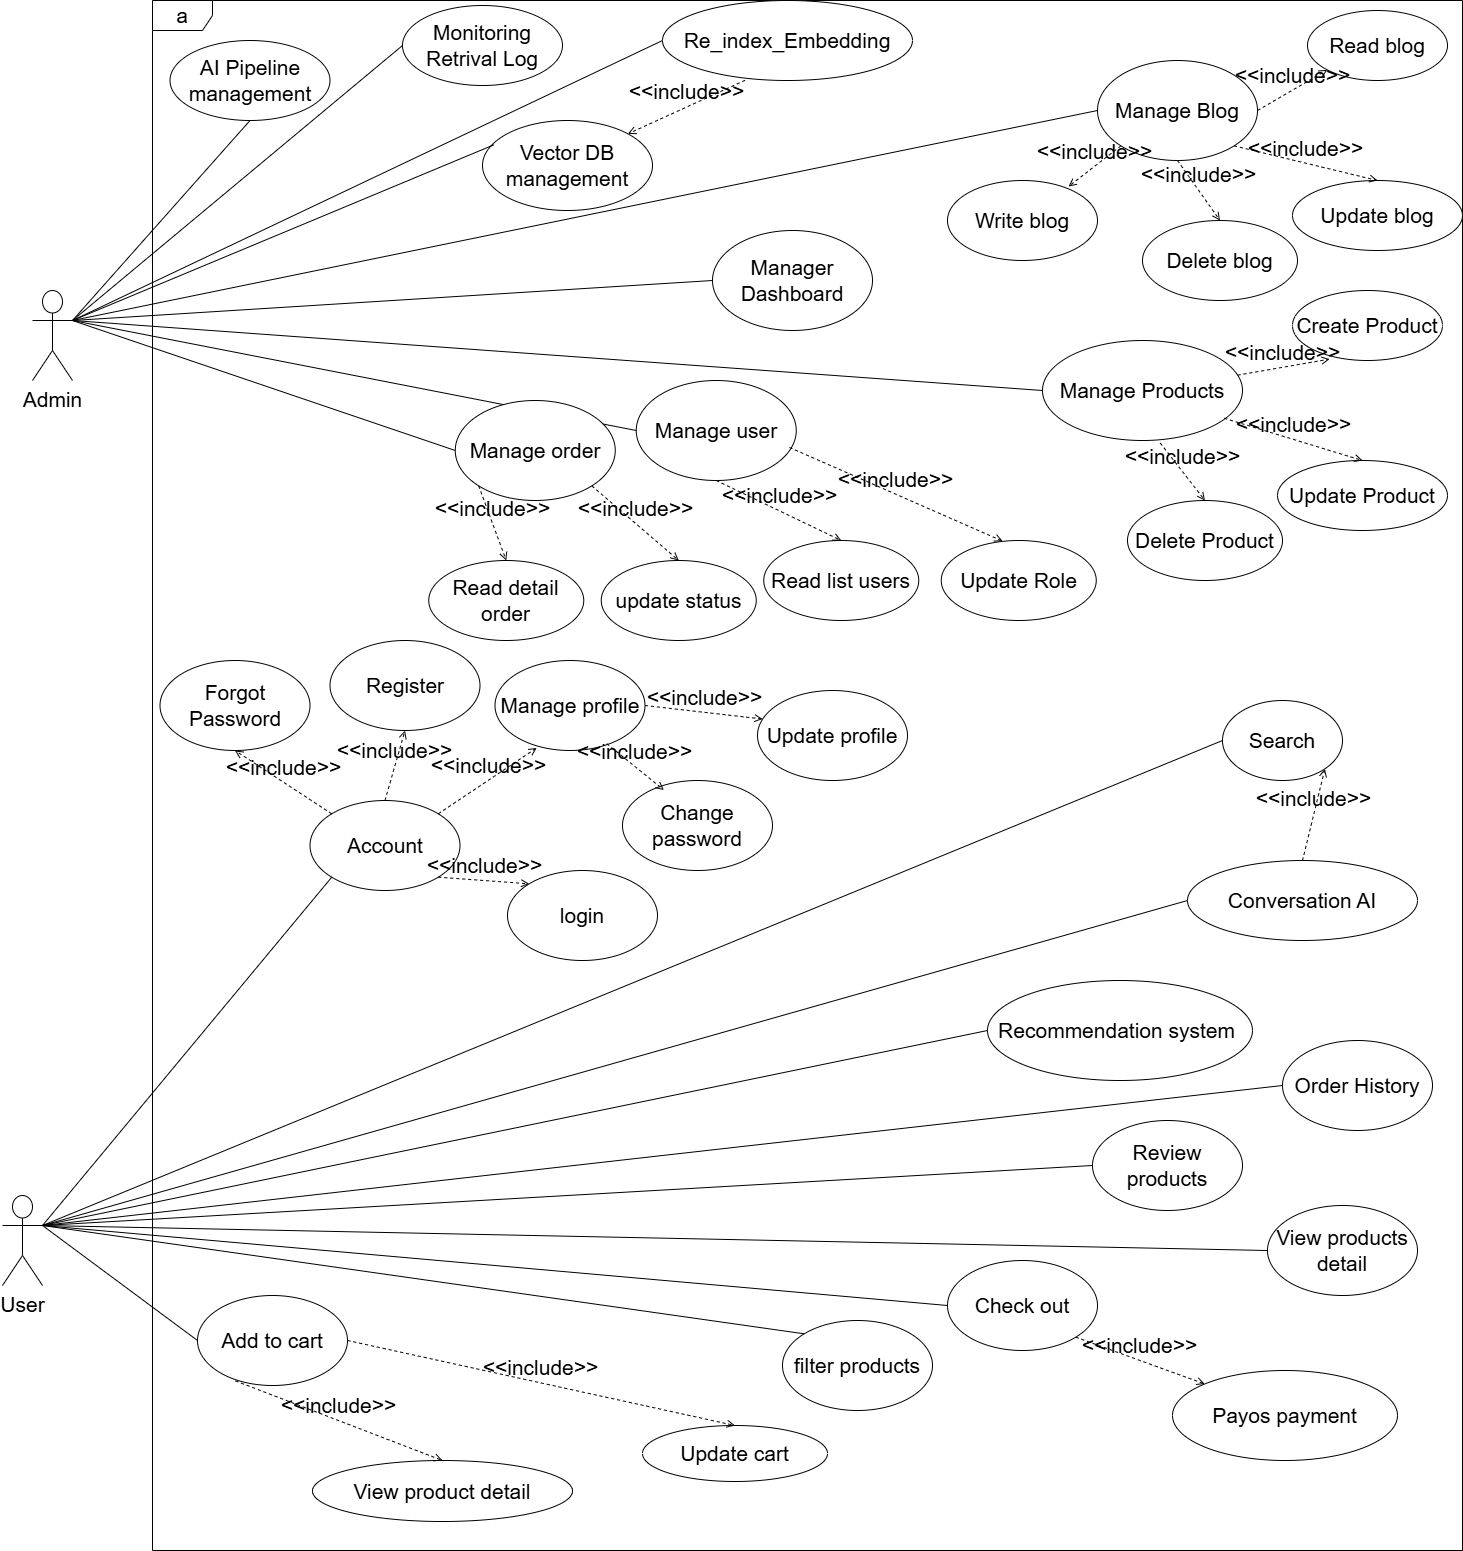
\includegraphics[width=0.9\linewidth]{Images/Usecase/usecase_DACN-Page-1.drawio.png}
%     \caption{Usecase toàn bộ hệ thống}
%     \label{fig:usecase-overall}
% \end{figure}



% Như trình bày ở Hình~\ref{fig:usecase-overall}, hệ thống thương mại điện tử AI bao gồm hai nhóm chức năng chính dành cho khách hàng và quản trị viên.

% Khách hàng có thể thực hiện các chức năng như đăng ký tài khoản, tìm kiếm sản phẩm, sử dụng AI Assistant để nhận tư vấn, xem sản phẩm gợi ý, thêm sản phẩm vào giỏ hàng, thanh toán và đánh giá sản phẩm.

% Quản trị viên chịu trách nhiệm quản lý dữ liệu hệ thống bao gồm quản lý sản phẩm, quản lý blog, quản lý người dùng, quản lý đơn hàng và quản lý AI Pipeline. Ngoài ra, hệ thống còn hỗ trợ Vector Database Management và Re-index Embedding để phục vụ cho chức năng tìm kiếm ngữ nghĩa và recommendation system.

% \subsubsection{Biểu đồ Use Case dành cho khách hàng}

% \begin{figure}[H]
%     \centering
%     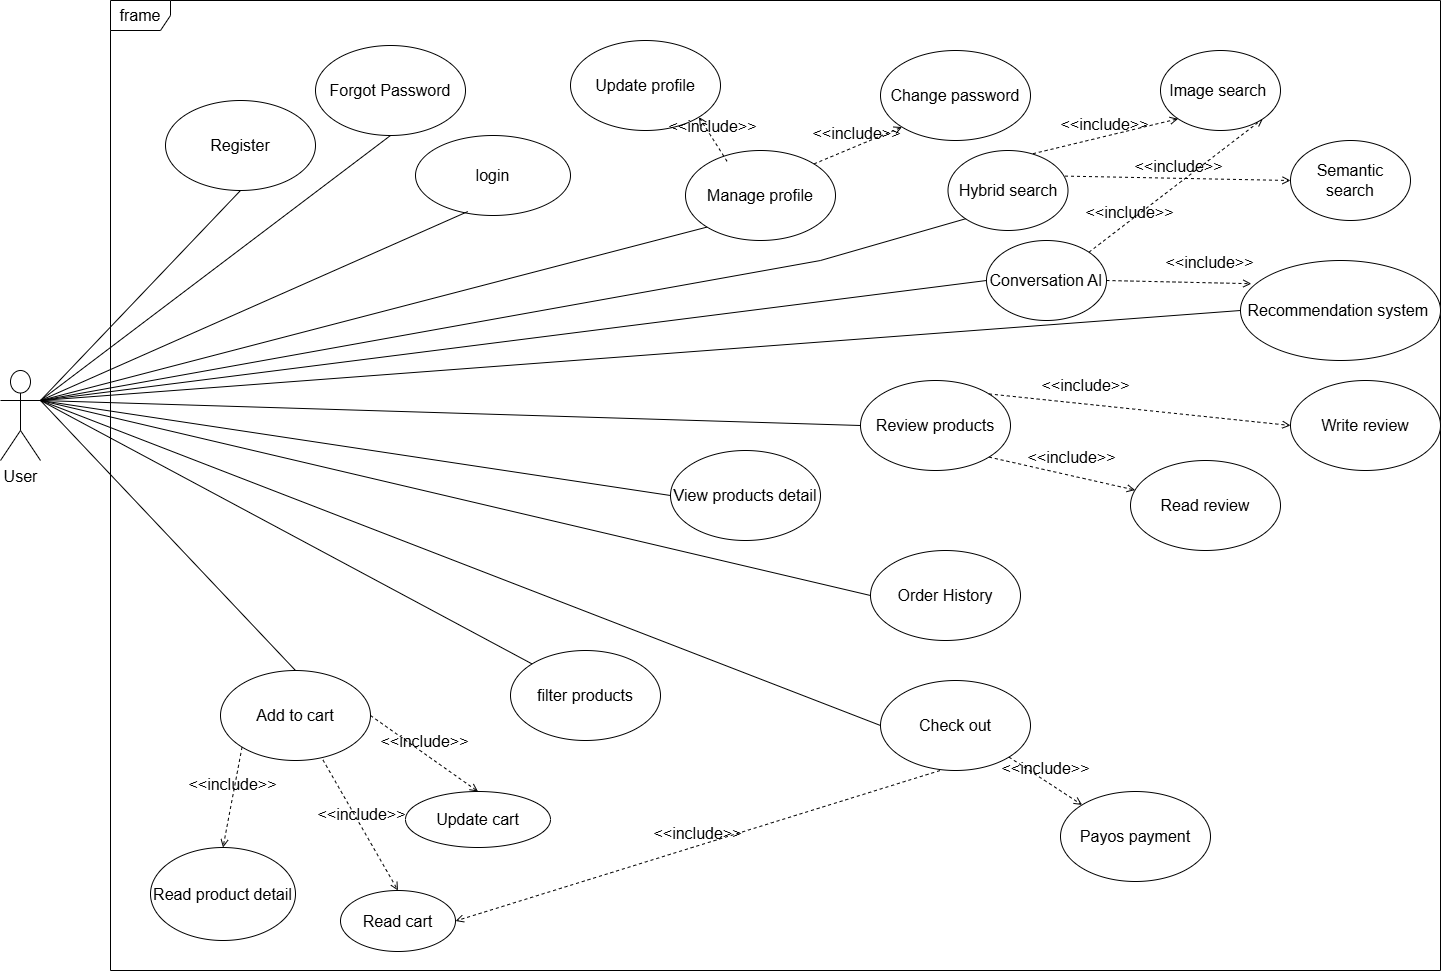
\includegraphics[width=0.9\linewidth]{Images/Usecase/usecase_DACN-Page-2.drawio.png}
%     \caption{Biểu đồ use case dành cho khách hàng}
%     \label{fig:usecase-customer}
% \end{figure}

% Như trình bày ở Hình~\ref{fig:usecase-user}, khách hàng có thể sử dụng các chức năng chính của hệ thống thương mại điện tử AI bao gồm quản lý tài khoản, tìm kiếm sản phẩm, sử dụng AI Assistant và thực hiện mua sắm trực tuyến.

% Hệ thống hỗ trợ nhiều phương thức tìm kiếm khác nhau như Semantic Search, Hybrid Search và Image Search nhằm nâng cao khả năng tìm kiếm sản phẩm theo nhu cầu người dùng.

% Ngoài ra, khách hàng có thể:
% \begin{itemize}
%     \item Đăng ký và đăng nhập hệ thống.
%     \item Quản lý hồ sơ cá nhân.
%     \item Thay đổi mật khẩu và cập nhật thông tin cá nhân.
%     \item Xem chi tiết sản phẩm.
%     \item Thêm sản phẩm vào giỏ hàng.
%     \item Cập nhật giỏ hàng.
%     \item Thanh toán đơn hàng thông qua cổng thanh toán PayOS.
%     \item Xem lịch sử đơn hàng.
%     \item Đánh giá sản phẩm sau khi mua.
%     \item Nhận gợi ý sản phẩm từ Recommendation System.
%     \item Tương tác với Conversation AI để nhận tư vấn mua sắm.
% \end{itemize}

% Trong đó, chức năng Hybrid Search bao gồm Semantic Search và Image Search nhằm hỗ trợ tìm kiếm sản phẩm bằng cả văn bản và hình ảnh. Recommendation System được tích hợp cùng Conversation AI để đề xuất các sản phẩm phù hợp với nhu cầu của khách hàng.

% \subsubsection{Biểu đồ Use Case dành cho quản trị viên}

% \begin{figure}[H]
%     \centering
%     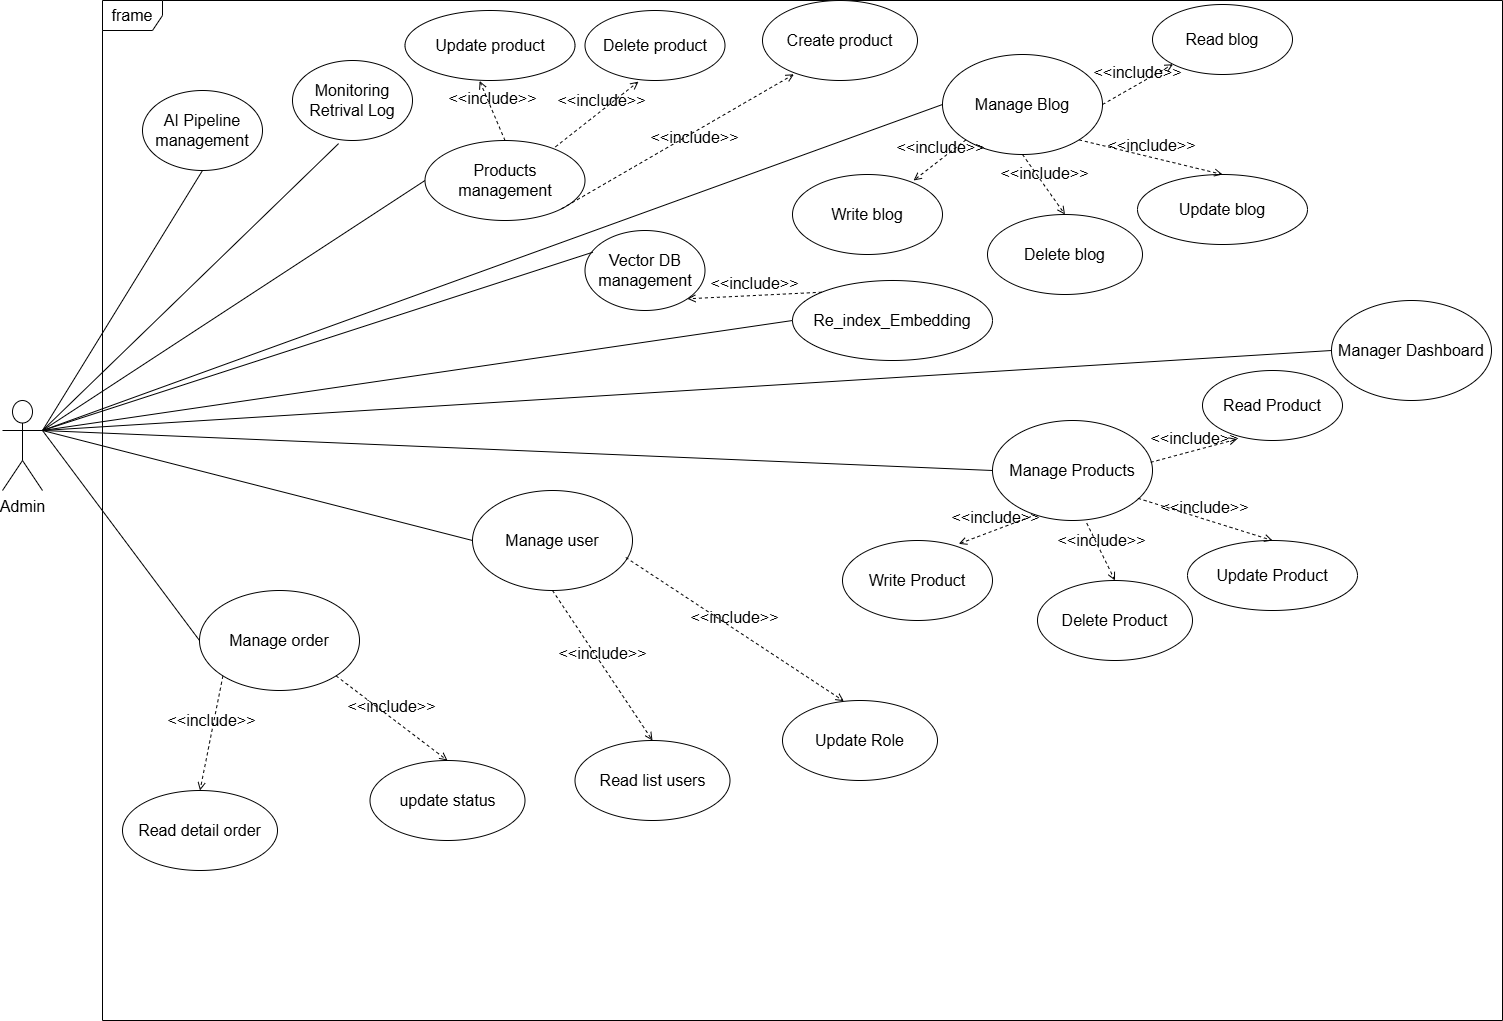
\includegraphics[width=0.9\linewidth]{Images/Usecase/usecase_DACN-Page-3.drawio.png}
%     \caption{Biểu đồ use case dành cho quản trị viên}
%     \label{fig:usecase-admin}
% \end{figure}

% Như trình bày ở Hình~\ref{fig:usecase-admin}, quản trị viên là tác nhân chịu trách nhiệm quản lý toàn bộ dữ liệu và hoạt động của hệ thống thương mại điện tử AI.

% Các chức năng chính của quản trị viên bao gồm:

% \begin{itemize}
%     \item Quản lý sản phẩm.
%     \item Quản lý người dùng.
%     \item Quản lý đơn hàng.
%     \item Quản lý blog.
%     \item Theo dõi dashboard hệ thống.
%     \item Quản lý AI Pipeline.
%     \item Theo dõi Monitoring Retrieval Log.
%     \item Quản lý Vector Database.
%     \item Thực hiện Re-index Embedding.
% \end{itemize}

% Trong chức năng quản lý sản phẩm, quản trị viên có thể thêm, sửa, xóa và xem danh sách sản phẩm.

% Đối với quản lý blog, hệ thống hỗ trợ tạo bài viết mới, chỉnh sửa bài viết, xóa bài viết và xem danh sách blog.

% Ngoài các chức năng quản trị thông thường, hệ thống còn hỗ trợ các chức năng liên quan đến AI như quản lý Vector Database và Re-index Embedding nhằm cập nhật dữ liệu embedding phục vụ cho Semantic Search, Recommendation System và Conversation AI.

% \subsubsection{Danh sách tác nhân}

% \begin{table}[H]
% \centering
% \caption{Danh sách tác nhân trong use case diagram}
% \label{tab:usecase-actors}
% \begin{tabularx}{\linewidth}{@{}p{0.25\linewidth}X@{}}
% \toprule
% \textbf{Tác nhân} & \textbf{Mô tả} \\
% \midrule
% Khách hàng & Người sử dụng hệ thống để tìm kiếm sản phẩm, nhận tư vấn từ assistant, xem sản phẩm gợi ý và lọc sản phẩm theo nhu cầu. \\
% Quản trị viên & Người quản lý sản phẩm và dữ liệu AI của hệ thống, có quyền thêm, xóa, sửa sản phẩm, đồng bộ dữ liệu sang AI Index và kiểm tra các tính năng liên quan đến AI Service. \\
% \bottomrule
% \end{tabularx}
% \end{table}


% % \end{table}

% \subsubsection{Mô tả các use case chính}

% \begin{table}[H]
% \centering
% \caption{Mô tả use case UC-US-01: Đăng nhập hệ thống}
% \label{tab:uc-login}
% \begin{tabularx}{\linewidth}{@{}p{0.28\linewidth}X@{}}
% \toprule
% \textbf{Thuộc tính} & \textbf{Mô tả} \\
% \midrule
% Mã use case & UC-US-01 \\
% Tên use case & Đăng nhập hệ thống \\
% Tác nhân & Khách hàng \\
% Tiền điều kiện & Người dùng đã có tài khoản trong hệ thống. \\
% Luồng chính &
% {
%  1/ Người dùng truy cập trang đăng nhập.

%  2/ Người dùng nhập email và mật khẩu.

%  3/ Hệ thống kiểm tra thông tin đăng nhập.

%  4/ Hệ thống xác thực thành công và chuyển đến trang chính.
% } \\
% Ngoại lệ &
% {
% 1/ Sai email hoặc mật khẩu.

% 2/ Tài khoản chưa được kích hoạt.
%  }\\
% Hậu điều kiện & Người dùng đăng nhập thành công vào hệ thống. \\
% \bottomrule
% \end{tabularx}
% \end{table}




% \begin{table}[H]
% \centering
% \caption{Mô tả use case UC-US-02: Hybrid Search sản phẩm}
% \label{tab:uc-hybrid-search}
% \begin{tabularx}{\linewidth}{@{}p{0.28\linewidth}X@{}}
% \toprule
% \textbf{Thuộc tính} & \textbf{Mô tả} \\
% \midrule
% Mã use case & UC-US-02 \\
% Tên use case & Hybrid Search sản phẩm \\
% Tác nhân & Khách hàng \\
% Tiền điều kiện & Người dùng truy cập hệ thống tìm kiếm sản phẩm. \\
% Luồng chính &
% {
% 1/ Người dùng nhập nội dung tìm kiếm hoặc tải ảnh sản phẩm.

% 2/ Hệ thống gửi yêu cầu đến AI Search Server.

% 3/ AI Service thực hiện Semantic Search và Image Search.

% 4/ Hệ thống tổng hợp kết quả tìm kiếm.

% 5/ Danh sách sản phẩm phù hợp được hiển thị cho người dùng.
% } \\
% Ngoại lệ &
% {
% 1/Không tìm thấy sản phẩm phù hợp.

% 2/AI Service không phản hồi.
% } \\
% Hậu điều kiện & Người dùng nhận được danh sách sản phẩm phù hợp với nhu cầu tìm kiếm. \\
% \bottomrule
% \end{tabularx}
% \end{table}




% \begin{table}[H]
% \centering
% \caption{Mô tả use case UC-US-03: Chat với Conversation AI}
% \label{tab:uc-conversation-ai}
% \begin{tabularx}{\linewidth}{@{}p{0.28\linewidth}X@{}}
% \toprule
% \textbf{Thuộc tính} & \textbf{Mô tả} \\
% \midrule
% Mã use case & UC-US-03 \\
% Tên use case & Chat với Conversation AI \\
% Tác nhân & Khách hàng \\
% Tiền điều kiện & Người dùng truy cập giao diện chat AI Assistant. \\
% Luồng chính &
% {
% 1/ Người dùng nhập câu hỏi hoặc nhu cầu mua sắm.

% 2/ Hệ thống gửi nội dung đến AI Service.

% 3/ Conversation AI xử lý yêu cầu.

% 4/ Recommendation System đề xuất sản phẩm phù hợp.

% 5/ Hệ thống hiển thị câu trả lời và danh sách sản phẩm gợi ý.
% } \\
% Ngoại lệ &
% {
%  1/ Nội dung không hợp lệ.

%  2/ AI Service không phản hồi.
% } \\
% Hậu điều kiện & Người dùng nhận được câu trả lời và sản phẩm gợi ý từ AI Assistant. \\
% \bottomrule
% \end{tabularx}
% \end{table}


% \begin{table}[H]
% \centering
% \caption{Mô tả use case UC-US-04: Thêm sản phẩm vào giỏ hàng}
% \label{tab:uc-add-cart}
% \begin{tabularx}{\linewidth}{@{}p{0.28\linewidth}X@{}}
% \toprule
% \textbf{Thuộc tính} & \textbf{Mô tả} \\
% \midrule
% Mã use case & UC-US-04 \\
% Tên use case & Thêm sản phẩm vào giỏ hàng \\
% Tác nhân & Khách hàng \\
% Tiền điều kiện & Người dùng đang xem chi tiết sản phẩm. \\
% Luồng chính &
% \begin{enumerate}
%     \item Người dùng chọn số lượng sản phẩm.
%     \item Người dùng nhấn nút thêm vào giỏ hàng.
%     \item Hệ thống kiểm tra tồn kho sản phẩm.
%     \item Hệ thống cập nhật giỏ hàng.
% \end{enumerate} \\
% Ngoại lệ &
% \begin{itemize}
%     \item Sản phẩm hết hàng.
%     \item Người dùng chưa đăng nhập.
% \end{itemize} \\
% Hậu điều kiện & Sản phẩm được thêm vào giỏ hàng thành công. \\
% \bottomrule
% \end{tabularx}
% \end{table}



% \begin{table}[H]
% \centering
% \caption{Mô tả use case UC-KH-03: Xem sản phẩm gợi ý}
% \label{tab:uc-product-suggestion}
% \begin{tabularx}{\linewidth}{@{}p{0.25\linewidth}X@{}}
% \toprule
% \textbf{Thuộc tính} & \textbf{Mô tả} \\
% \midrule
% Mã use case & UC-KH-03 \\
% Tên use case & Xem sản phẩm gợi ý \\
% Tác nhân & Khách hàng \\
% Tiền điều kiện & Hệ thống đã có danh sách sản phẩm gợi ý từ kết quả tìm kiếm hoặc từ assistant. \\
% Luồng chính & Hệ thống lấy danh sách sản phẩm gợi ý; hệ thống lấy thông tin chi tiết của từng sản phẩm; hệ thống hiển thị sản phẩm dưới dạng danh sách hoặc thẻ sản phẩm; khách hàng xem thông tin sản phẩm được đề xuất. \\
% Ngoại lệ & Sản phẩm gợi ý không còn tồn tại, đã hết hàng hoặc không khả dụng. \\
% Hậu điều kiện & Khách hàng xem được danh sách sản phẩm được đề xuất. \\
% \bottomrule
% \end{tabularx}
% \end{table}




% \begin{table}[H]
% \centering
% \caption{Mô tả use case UC-AD-01: Thêm xóa sửa sản phẩm}
% \label{tab:uc-admin-crud-product}
% \begin{tabularx}{\linewidth}{@{}p{0.25\linewidth}X@{}}
% \toprule
% \textbf{Thuộc tính} & \textbf{Mô tả} \\
% \midrule
% Mã use case & UC-AD-01 \\
% Tên use case & Thêm xóa sửa sản phẩm \\
% Tác nhân & Quản trị viên \\
% Tiền điều kiện & Quản trị viên đã đăng nhập vào hệ thống và có quyền quản lý sản phẩm. \\
% Luồng chính & Quản trị viên truy cập chức năng quản lý sản phẩm; quản trị viên chọn thao tác thêm, xóa hoặc sửa sản phẩm; hệ thống hiển thị biểu mẫu hoặc thông tin sản phẩm; quản trị viên nhập hoặc cập nhật thông tin; hệ thống kiểm tra dữ liệu và lưu thay đổi. \\
% Ngoại lệ & Dữ liệu sản phẩm không hợp lệ, thiếu thông tin bắt buộc hoặc thao tác cập nhật thất bại. \\
% Hậu điều kiện & Thông tin sản phẩm trong hệ thống được thêm mới, cập nhật hoặc xóa theo thao tác của quản trị viên. \\
% \bottomrule
% \end{tabularx}
% \end{table}


% \begin{table}[H]
% \centering
% \caption{Mô tả use case UC-US-04: Thêm sản phẩm vào giỏ hàng}
% \label{tab:uc-add-cart}
% \begin{tabularx}{\linewidth}{@{}p{0.28\linewidth}X@{}}
% \toprule
% \textbf{Thuộc tính} & \textbf{Mô tả} \\
% \midrule
% Mã use case & UC-US-04 \\
% Tên use case & Thêm sản phẩm vào giỏ hàng \\
% Tác nhân & Khách hàng \\
% Tiền điều kiện & Người dùng đang xem chi tiết sản phẩm. \\
% Luồng chính &
% \begin{enumerate}
%     \item Người dùng chọn số lượng sản phẩm.
%     \item Người dùng nhấn nút thêm vào giỏ hàng.
%     \item Hệ thống kiểm tra tồn kho sản phẩm.
%     \item Hệ thống cập nhật giỏ hàng.
% \end{enumerate} \\
% Ngoại lệ &
% \begin{itemize}
%     \item Sản phẩm hết hàng.
%     \item Người dùng chưa đăng nhập.
% \end{itemize} \\
% Hậu điều kiện & Sản phẩm được thêm vào giỏ hàng thành công. \\
% \bottomrule
% \end{tabularx}
% \end{table}




% \begin{table}[H]
% \centering
% \caption{Mô tả use case UC-US-05: Thanh toán đơn hàng}
% \label{tab:uc-checkout}
% \begin{tabularx}{\linewidth}{@{}p{0.28\linewidth}X@{}}
% \toprule
% \textbf{Thuộc tính} & \textbf{Mô tả} \\
% \midrule
% Mã use case & UC-US-05 \\
% Tên use case & Thanh toán đơn hàng \\
% Tác nhân & Khách hàng \\
% Tiền điều kiện & Giỏ hàng có ít nhất một sản phẩm. \\
% Luồng chính &
% \begin{enumerate}
%     \item Người dùng truy cập trang checkout.
%     \item Hệ thống hiển thị thông tin đơn hàng.
%     \item Người dùng nhập thông tin giao hàng.
%     \item Người dùng chọn phương thức thanh toán.
%     \item Hệ thống chuyển sang cổng thanh toán PayOS.
%     \item Thanh toán thành công.
% \end{enumerate} \\
% Ngoại lệ &
% \begin{itemize}
%     \item Thanh toán thất bại.
%     \item Người dùng hủy giao dịch.
% \end{itemize} \\
% Hậu điều kiện & Đơn hàng được tạo thành công trong hệ thống. \\
% \bottomrule
% \end{tabularx}
% \end{table}

\subsection{Phân tích ca sử dụng}

Phần này đặc tả chi tiết các ca sử dụng có luồng giao dịch, chuyển trạng thái hoặc xử lý AI đặc trưng. Các thao tác còn lại được tổng hợp theo nhóm để bảo đảm khả năng truy vết mà không lặp lại nội dung đã thể hiện trên biểu đồ và các sơ đồ hành vi.

\newcommand{\UseCaseSpecification}[7]{%
    \begin{table}[!htbp]
        \centering
        \caption{Đặc tả #1 -- #2}
        \begin{tabularx}{\textwidth}{|p{0.25\textwidth}|X|}
            \hline
            \textbf{Tác nhân} & #3 \\ \hline
            \textbf{Tiền điều kiện và kích hoạt} & #4 \\ \hline
            \textbf{Luồng chính} & #5 \\ \hline
            \textbf{Luồng thay thế/ngoại lệ} & #6 \\ \hline
            \textbf{Hậu điều kiện} & #7 \\ \hline
        \end{tabularx}
    \end{table}
}

\subsubsection{Tác nhân của hệ thống}

\begin{table}[!htbp]
    \centering
    \caption{Các tác nhân tham gia hệ thống}
    \label{tab:usecase-actors}
    \begin{tabularx}{\textwidth}{|p{0.22\textwidth}|X|}
        \hline
        \textbf{Tác nhân} & \textbf{Vai trò} \\ \hline
        Khách vãng lai & Tra cứu sản phẩm, bài viết và sử dụng các chức năng tìm kiếm công khai. \\ \hline
        Khách hàng & Quản lý tài khoản, giỏ hàng, đơn hàng và tương tác với trợ lý AI. \\ \hline
        Quản trị viên & Quản trị danh mục, sản phẩm, tồn kho, đơn hàng, nội dung và vận hành dữ liệu AI. \\ \hline
        Dịch vụ AI & Thực hiện tìm kiếm ngữ nghĩa, tìm kiếm ảnh/kết hợp, hội thoại RAG và quản lý chỉ mục vector. \\ \hline
    \end{tabularx}
\end{table}

\subsubsection{Ca sử dụng của khách hàng}

\begin{figure}[!htbp]
    \centering
    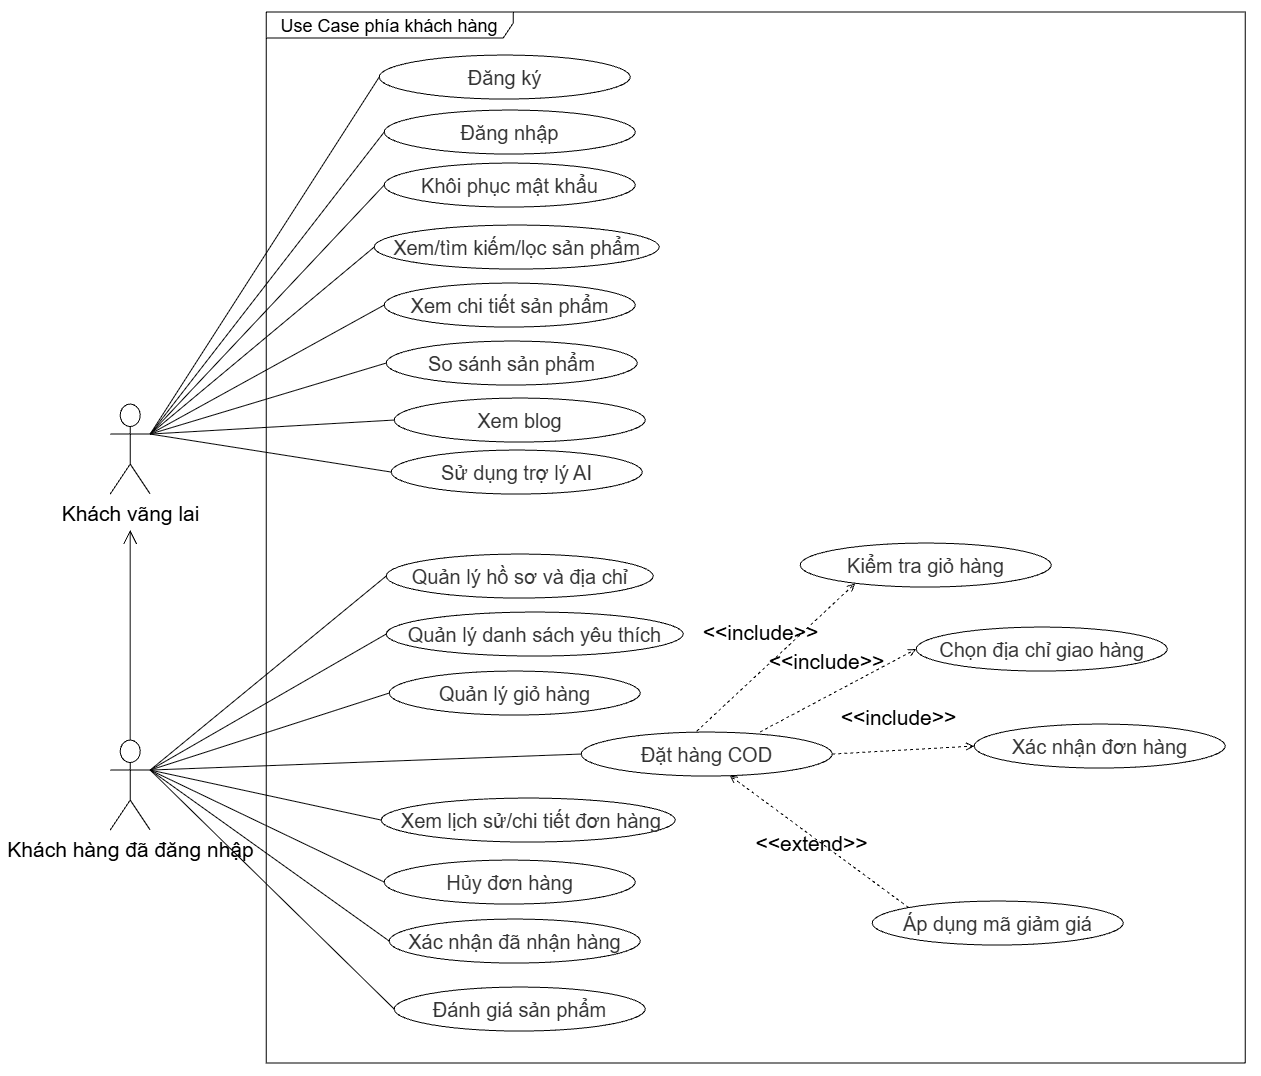
\includegraphics[width=0.94\textwidth]{Images/Usecase/da-Use Case phía khách hàng.drawio.png}
    \caption{Biểu đồ ca sử dụng phía khách hàng}
    \label{fig:usecase-customer}
\end{figure}

\begin{longtable}{|p{0.10\textwidth}|p{0.18\textwidth}|p{0.15\textwidth}|p{0.20\textwidth}|p{0.24\textwidth}|}
    \caption{Danh mục ca sử dụng phía khách hàng}\label{tab:usecase-customer-summary}\\
    \hline
    \textbf{Mã} & \textbf{Tên ca sử dụng} & \textbf{Tác nhân} & \textbf{Mục tiêu} & \textbf{Điều kiện/Kết quả chính} \\ \hline
    \endfirsthead
    \hline
    \textbf{Mã} & \textbf{Tên ca sử dụng} & \textbf{Tác nhân} & \textbf{Mục tiêu} & \textbf{Điều kiện/Kết quả chính} \\ \hline
    \endhead
    UC-KH-01 & Đăng ký & Khách vãng lai & Tạo tài khoản mới & Thông tin hợp lệ; tài khoản được tạo và xác thực. \\ \hline
    UC-KH-02 & Đăng nhập & Khách vãng lai & Truy cập chức năng cá nhân & Thông tin đúng; phiên đăng nhập được thiết lập. \\ \hline
    UC-KH-03 & Khôi phục mật khẩu & Khách vãng lai & Cấp lại quyền truy cập & Email tồn tại; mật khẩu được đặt lại an toàn. \\ \hline
    UC-KH-04 & Xem danh mục & Mọi khách hàng & Duyệt danh mục sản phẩm & Danh mục khả dụng; danh sách được hiển thị. \\ \hline
    UC-KH-05 & Tìm kiếm truyền thống & Mọi khách hàng & Tìm theo từ khóa và bộ lọc & Truy vấn hợp lệ; trả về sản phẩm phù hợp. \\ \hline
    UC-KH-06 & Xem chi tiết sản phẩm & Mọi khách hàng & Xem biến thể, giá và tồn kho & Sản phẩm còn hoạt động; dữ liệu hiện hành được hiển thị. \\ \hline
    UC-KH-07 & So sánh sản phẩm & Mọi khách hàng & Đối chiếu thuộc tính & Có các sản phẩm hợp lệ; bảng so sánh được tạo. \\ \hline
    UC-KH-08 & Xem bài viết & Mọi khách hàng & Tra cứu nội dung tư vấn & Bài viết đã xuất bản; nội dung được hiển thị. \\ \hline
    UC-KH-09 & Quản lý hồ sơ, địa chỉ và yêu thích & Khách hàng & Cập nhật dữ liệu cá nhân & Đã đăng nhập; dữ liệu được lưu đúng quyền sở hữu. \\ \hline
    UC-KH-10 & Quản lý giỏ hàng & Khách hàng & Thêm, sửa, xóa sản phẩm & Biến thể hợp lệ; giỏ phản ánh giá và tồn kho hiện hành. \\ \hline
    UC-KH-11 & Đặt hàng COD & Khách hàng & Tạo đơn thanh toán khi nhận hàng & Giỏ và địa chỉ hợp lệ; đơn COD được tạo. \\ \hline
    UC-KH-12 & Xem lịch sử đơn hàng & Khách hàng & Theo dõi đơn đã đặt & Đã đăng nhập; chỉ hiển thị đơn thuộc khách hàng. \\ \hline
    UC-KH-13 & Hủy đơn hàng & Khách hàng & Hủy đơn còn cho phép & Đơn đúng chủ và đúng trạng thái; tồn kho được hoàn trả. \\ \hline
    UC-KH-14 & Xác nhận nhận hàng & Khách hàng & Hoàn tất đơn đã giao & Đơn đang giao; trạng thái được chuyển hoàn tất. \\ \hline
    UC-KH-15 & Đánh giá sản phẩm & Khách hàng & Gửi nhận xét sau mua & Đơn đã hoàn tất; đánh giá được ghi nhận để kiểm duyệt. \\ \hline
    UC-KH-16 & Sử dụng trợ lý AI & Mọi khách hàng & Truy cập nhóm chức năng AI & Yêu cầu hợp lệ; chuyển tới ca sử dụng AI tương ứng. \\ \hline
\end{longtable}

\UseCaseSpecification{UC-KH-10}{Quản lý giỏ hàng}
{Khách hàng đã đăng nhập}
{Biến thể sản phẩm đang hoạt động; khách hàng thêm sản phẩm hoặc thay đổi số lượng trong giỏ.}
{Hệ thống lấy giỏ hiện tại, kiểm tra biến thể, giá và tồn kho; sau đó thêm, cập nhật hoặc xóa dòng hàng và tính lại tổng tiền.}
{Số lượng bằng không được hiểu là xóa; từ chối khi biến thể không hợp lệ, vượt tồn kho hoặc giỏ không thuộc khách hàng.}
{Giỏ hàng nhất quán với giá, biến thể và số lượng có thể bán tại thời điểm cập nhật.}

\UseCaseSpecification{UC-KH-11}{Đặt hàng COD}
{Khách hàng đã đăng nhập}
{Giỏ có sản phẩm hợp lệ và còn hàng; khách hàng đã chọn địa chỉ rồi xác nhận thanh toán COD.}
{Hệ thống kiểm tra lại giỏ và tồn kho, áp dụng mã giảm giá nếu có, tính tổng tiền, tạo đơn cùng chi tiết đơn và bản ghi thanh toán COD.}
{Khách hàng có thể bỏ mã giảm giá; hệ thống dừng khi giỏ rỗng, hết hàng, địa chỉ hoặc mã không hợp lệ, hay giao dịch tạo đơn thất bại.}
{Đơn COD được tạo một lần, dữ liệu giá được chốt và tồn kho được cập nhật theo quy tắc nghiệp vụ.}

\UseCaseSpecification{UC-KH-13}{Hủy đơn hàng}
{Khách hàng đã đăng nhập}
{Đơn thuộc khách hàng và đang ở trạng thái cho phép hủy; khách hàng gửi yêu cầu hủy.}
{Hệ thống khóa và kiểm tra đơn, chuyển trạng thái sang đã hủy, hoàn phần tồn kho liên quan và ghi lịch sử thay đổi.}
{Từ chối nếu đơn không thuộc khách hàng, đã qua giai đoạn cho phép hủy hoặc vừa được tiến trình khác cập nhật.}
{Đơn ở trạng thái đã hủy; tồn kho và lịch sử trạng thái được cập nhật nhất quán.}

\subsubsection{Ca sử dụng của quản trị viên}

\begin{figure}[!htbp]
    \centering
    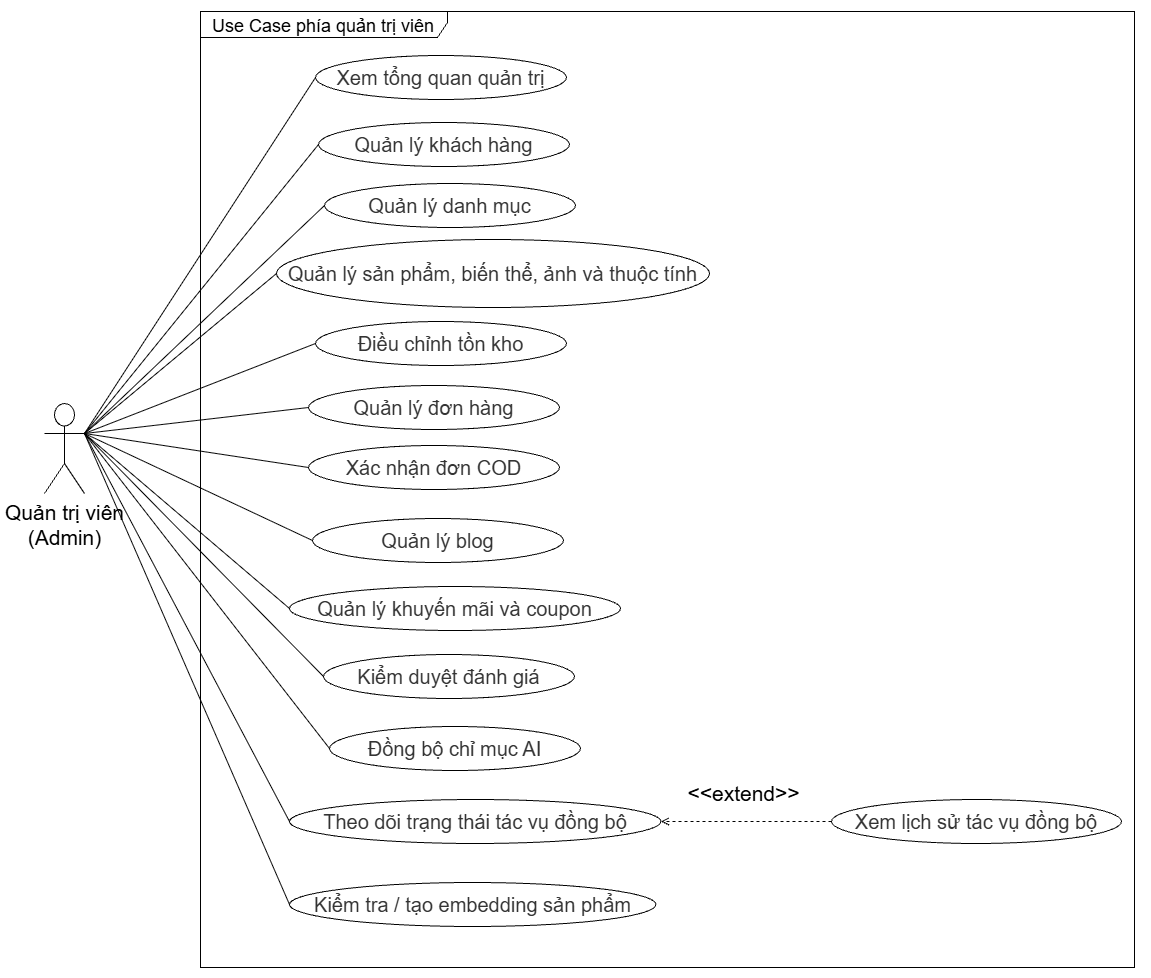
\includegraphics[width=0.92\textwidth]{Images/Usecase/da-Use Case phía quản trị viên.drawio.png}
    \caption{Biểu đồ ca sử dụng phía quản trị viên}
    \label{fig:usecase-admin}
\end{figure}

\begin{longtable}{|p{0.10\textwidth}|p{0.18\textwidth}|p{0.15\textwidth}|p{0.20\textwidth}|p{0.24\textwidth}|}
    \caption{Danh mục ca sử dụng phía quản trị viên}\label{tab:usecase-admin-summary}\\
    \hline
    \textbf{Mã} & \textbf{Tên ca sử dụng} & \textbf{Tác nhân} & \textbf{Mục tiêu} & \textbf{Điều kiện/Kết quả chính} \\ \hline
    \endfirsthead
    \hline
    \textbf{Mã} & \textbf{Tên ca sử dụng} & \textbf{Tác nhân} & \textbf{Mục tiêu} & \textbf{Điều kiện/Kết quả chính} \\ \hline
    \endhead
    UC-AD-01 & Xem dashboard & Quản trị viên & Theo dõi chỉ số vận hành & Có quyền truy cập; số liệu tổng hợp được hiển thị. \\ \hline
    UC-AD-02 & Quản lý khách hàng & Quản trị viên & Tra cứu và cập nhật trạng thái tài khoản & Có quyền quản trị; thay đổi được lưu và ghi nhận. \\ \hline
    UC-AD-03 & Quản lý danh mục & Quản trị viên & Tổ chức cây danh mục & Dữ liệu hợp lệ; cấu trúc danh mục được cập nhật. \\ \hline
    UC-AD-04 & Quản lý sản phẩm & Quản trị viên & Quản lý sản phẩm, biến thể và thuộc tính & Có quyền danh mục; dữ liệu được lưu và đánh dấu đồng bộ AI. \\ \hline
    UC-AD-05 & Điều chỉnh tồn kho & Quản trị viên & Điều chỉnh số lượng có thể bán & Biến thể tồn tại; tồn kho và lịch sử được cập nhật. \\ \hline
    UC-AD-06 & Quản lý đơn hàng & Quản trị viên & Tra cứu và xử lý vòng đời đơn & Có quyền đơn hàng; trạng thái tuân thủ quy tắc chuyển đổi. \\ \hline
    UC-AD-07 & Xác nhận đơn COD & Quản trị viên & Xác nhận đơn đủ điều kiện xử lý & Đơn COD và tồn kho hợp lệ; giao dịch được ghi nhận. \\ \hline
    UC-AD-08 & Quản lý bài viết & Quản trị viên & Soạn và xuất bản nội dung & Nội dung hợp lệ; trạng thái xuất bản được cập nhật. \\ \hline
    UC-AD-09 & Quản lý khuyến mãi & Quản trị viên & Cấu hình chương trình giảm giá & Điều kiện và thời gian hợp lệ; chương trình được lưu. \\ \hline
    UC-AD-10 & Kiểm duyệt đánh giá & Quản trị viên & Duyệt hoặc ẩn phản hồi & Có quyền kiểm duyệt; trạng thái đánh giá được cập nhật. \\ \hline
\end{longtable}

Các tác vụ vận hành AI trước đây ký hiệu UC-AD-11, UC-AD-12 và UC-AD-13 được quy về UC-AI-07, UC-AI-08 và UC-AI-09. Cách biểu diễn này giữ quan hệ quản trị viên khởi tạo tác vụ nhưng tránh đặc tả trùng lặp ở hai nhóm.

\UseCaseSpecification{UC-AD-04}{Quản lý sản phẩm}
{Quản trị viên có quyền quản lý danh mục}
{Sản phẩm hoặc danh mục liên quan tồn tại khi cập nhật; quản trị viên tạo mới hoặc chỉnh sửa sản phẩm.}
{Hệ thống kiểm tra dữ liệu chính, biến thể, ảnh và thuộc tính; lưu các thay đổi trong một giao dịch và đánh dấu dữ liệu cần đồng bộ sang chỉ mục AI.}
{Có thể cập nhật từng thành phần độc lập; từ chối SKU trùng, giá hoặc biến thể không hợp lệ, lỗi tải ảnh hay lỗi giao dịch.}
{Dữ liệu sản phẩm nhất quán và trạng thái đồng bộ AI được ghi nhận để xử lý tiếp.}

\UseCaseSpecification{UC-AD-07}{Xác nhận đơn COD}
{Quản trị viên có quyền xử lý đơn hàng}
{Đơn sử dụng COD, đang ở trạng thái có thể xác nhận và còn đủ tồn kho; quản trị viên chọn xác nhận.}
{Hệ thống khóa đơn, kiểm tra thanh toán và tồn kho, xác nhận đơn, cập nhật trạng thái liên quan, đồng thời ghi giao dịch kho và lịch sử xử lý.}
{Từ chối khi đơn không phải COD, thiếu tồn kho, đã được xử lý hoặc giao dịch cập nhật thất bại.}
{Đơn chuyển sang trạng thái xử lý kế tiếp; thanh toán, tồn kho và lịch sử trạng thái nhất quán.}

\subsubsection{Ca sử dụng của AI Service}

\begin{figure}[!htbp]
    \centering
    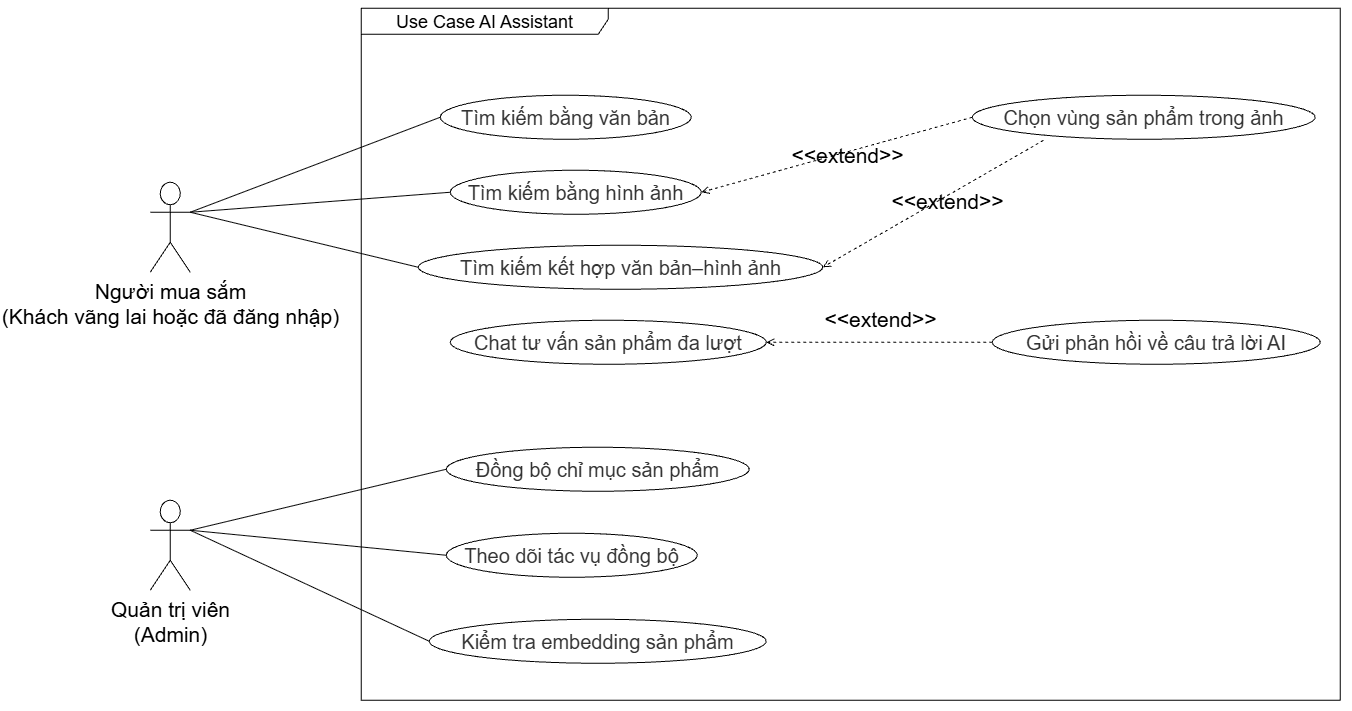
\includegraphics[width=\linewidth]{Images/Usecase/da-Use Case AI Assistant.drawio.png}
    \caption{Biểu đồ ca sử dụng của AI Service}
    \label{fig:usecase-ai-assistant}
\end{figure}

\begin{longtable}{|p{0.10\textwidth}|p{0.18\textwidth}|p{0.15\textwidth}|p{0.20\textwidth}|p{0.24\textwidth}|}
    \caption{Danh mục ca sử dụng của AI Service}\label{tab:usecase-ai-summary}\\
    \hline
    \textbf{Mã} & \textbf{Tên ca sử dụng} & \textbf{Tác nhân} & \textbf{Mục tiêu} & \textbf{Điều kiện/Kết quả chính} \\ \hline
    \endfirsthead
    \hline
    \textbf{Mã} & \textbf{Tên ca sử dụng} & \textbf{Tác nhân} & \textbf{Mục tiêu} & \textbf{Điều kiện/Kết quả chính} \\ \hline
    \endhead
    UC-AI-01 & Tìm kiếm văn bản & Người mua & Tìm sản phẩm theo ngữ nghĩa & Truy vấn hợp lệ; trả về danh sách đã xếp hạng. \\ \hline
    UC-AI-02 & Tìm kiếm hình ảnh & Người mua & Tìm sản phẩm tương tự ảnh & Ảnh hợp lệ và chỉ mục sẵn sàng; trả về kết quả tương tự. \\ \hline
    UC-AI-03 & Tìm kiếm kết hợp & Người mua & Kết hợp tín hiệu văn bản và ảnh & Có ít nhất một tín hiệu hợp lệ; kết quả được hợp nhất và xếp hạng. \\ \hline
    UC-AI-04 & Chat tư vấn đa lượt & Người mua & Nhận tư vấn dựa trên dữ liệu sản phẩm & Phiên hợp lệ; phản hồi có ngữ cảnh và được lưu vào hội thoại. \\ \hline
    UC-AI-05 & Chọn vùng ảnh & Người mua & Giới hạn đối tượng cần tìm & Vùng chọn hợp lệ; được xử lý như luồng mở rộng của UC-AI-02/03. \\ \hline
    UC-AI-06 & Gửi phản hồi AI & Khách hàng & Ghi nhận mức hữu ích của kết quả & Có kết quả hoặc hội thoại; phản hồi được lưu để đánh giá. \\ \hline
    UC-AI-07 & Đồng bộ chỉ mục & Quản trị viên & Cập nhật vector theo dữ liệu nghiệp vụ & Có quyền vận hành; tác vụ đồng bộ được tạo và thực thi. \\ \hline
    UC-AI-08 & Theo dõi tác vụ đồng bộ & Quản trị viên & Theo dõi tiến độ và lỗi & Có mã tác vụ; trạng thái và thống kê được hiển thị. \\ \hline
    UC-AI-09 & Kiểm tra embedding & Quản trị viên & Kiểm tra độ đầy đủ của chỉ mục & Chỉ mục truy cập được; báo cáo sai lệch được tạo. \\ \hline
\end{longtable}

\UseCaseSpecification{UC-AI-02}{Tìm kiếm hình ảnh}
{Người mua}
{Ảnh đúng định dạng, dung lượng cho phép và chỉ mục ảnh sẵn sàng; người mua tải ảnh hoặc chọn vùng ảnh để tìm kiếm.}
{Dịch vụ kiểm tra và giải mã ảnh, dùng ảnh gốc hoặc vùng chọn để sinh embedding, truy hồi và xếp hạng vector, rồi ánh xạ sang dữ liệu sản phẩm hiện hành.}
{Không chọn vùng thì dùng ảnh gốc hoặc vùng được phát hiện tự động; trả lỗi có kiểm soát khi ảnh hỏng, dịch vụ hoặc chỉ mục không sẵn sàng.}
{Danh sách sản phẩm tương tự, hoặc kết quả rỗng có giải thích, được trả về cho giao diện.}

\UseCaseSpecification{UC-AI-03}{Tìm kiếm kết hợp}
{Người mua}
{Có văn bản và ảnh hợp lệ, các chỉ mục liên quan sẵn sàng; người mua gửi yêu cầu tìm kiếm kết hợp.}
{Dịch vụ phân tích hai tín hiệu, truy hồi theo văn bản và ảnh, hợp nhất điểm, áp dụng bộ lọc, xếp hạng rồi lấy dữ liệu sản phẩm hiện hành.}
{Nếu một nhánh thất bại, hệ thống có thể dùng nhánh còn lại và kèm cảnh báo; yêu cầu thất bại khi cả hai tín hiệu không hợp lệ hoặc đều không khả dụng.}
{Kết quả phản ánh đồng thời ý định văn bản và mức tương đồng hình ảnh trong phạm vi dữ liệu đang bán.}

\UseCaseSpecification{UC-AI-04}{Chat tư vấn đa lượt}
{Người mua}
{Phiên hội thoại hợp lệ và nội dung gửi lên được chấp nhận; người mua đặt câu hỏi hoặc bổ sung ràng buộc.}
{Dịch vụ đọc bộ nhớ hội thoại, nhận diện ý định và ràng buộc, truy hồi dữ liệu khi cần, sinh câu trả lời có căn cứ rồi cập nhật bộ nhớ phiên.}
{Dịch vụ hỏi lại khi yêu cầu mơ hồ; phản hồi an toàn khi ngoài phạm vi, không có sản phẩm phù hợp, hoặc mô hình và hệ truy hồi gặp lỗi.}
{Câu trả lời được trả về và ngữ cảnh cần thiết được lưu để tiếp tục hội thoại đa lượt.}

\FloatBarrier

\subsection{Sơ đồ hoạt động của hệ thống}

Các Activity Diagram mô tả trình tự thực hiện, điểm quyết định, luồng thay thế và trách nhiệm của từng thành phần trong những nghiệp vụ tiêu biểu. Khác với các sơ đồ pipeline kỹ thuật ở phần quy trình nghiệp vụ, nhóm sơ đồ này tập trung vào hành vi quan sát được từ lúc tác nhân khởi tạo yêu cầu đến khi hệ thống trả kết quả. Năm hoạt động được lựa chọn bao quát nghiệp vụ mua hàng COD, xử lý đơn, tìm kiếm đa phương thức, hội thoại tư vấn và vận hành chỉ mục AI.

\subsubsection{Hoạt động đặt hàng COD}

Hình~\ref{fig:activity-cod-checkout} cụ thể hóa UC-KH-11. Khách hàng mở giỏ hàng, chọn địa chỉ giao hàng và quyết định có sử dụng mã giảm giá hay không. Hệ thống kiểm tra giỏ hàng, tồn kho, địa chỉ và coupon trước khi tính tổng thanh toán. Chỉ khi khách hàng xác nhận và dữ liệu vẫn hợp lệ, hệ thống mới tạo đơn, chi tiết đơn và bản ghi thanh toán COD ở trạng thái chờ xác nhận. Nếu thao tác tạo đơn thất bại, giao dịch được rollback và không để lại đơn không hoàn chỉnh.

\begin{figure}[H]
    \centering
    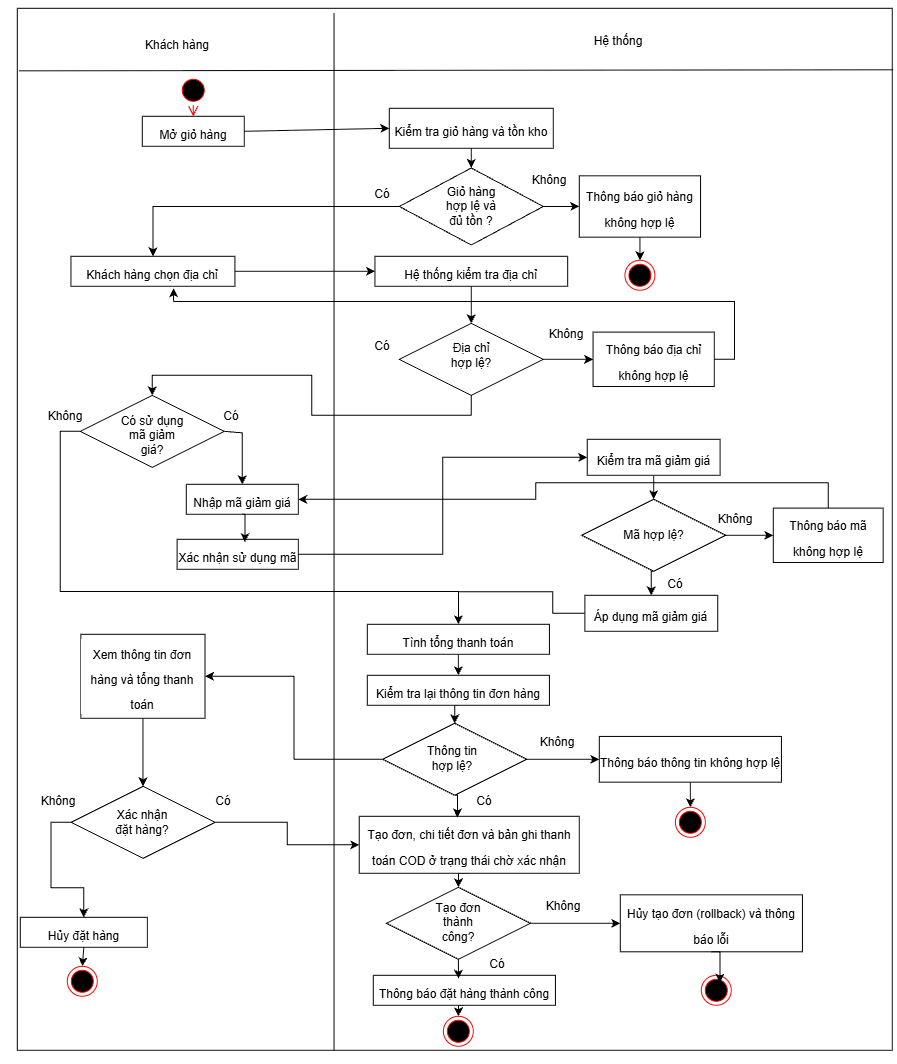
\includegraphics[width=\linewidth,height=0.82\textheight,keepaspectratio]{Images/Activity/da-Đặt hàng COD.drawio.png}
    \caption{Activity Diagram đặt hàng COD}
    \label{fig:activity-cod-checkout}
\end{figure}

Ở bước này hệ thống mới ghi nhận yêu cầu đặt hàng; việc cập nhật tồn kho được thực hiện khi quản trị viên xác nhận xử lý đơn. Sự phân tách này giúp tránh nhầm lẫn giữa thao tác đặt hàng của khách hàng và nghiệp vụ tiếp nhận đơn COD của quản trị viên.

\subsubsection{Hoạt động xử lý và xác nhận đơn COD}

Hình~\ref{fig:activity-cod-confirmation} mô tả UC-AD-06 và UC-AD-07. Sau khi quản trị viên chọn một đơn chờ xác nhận, hệ thống kiểm tra phương thức thanh toán và trạng thái đơn, khóa dữ liệu liên quan rồi kiểm tra lại tồn kho. Việc cập nhật trạng thái đơn, tồn kho, biến động kho và lịch sử xử lý được thực hiện trong cùng một giao dịch. Khi một bước thất bại, hệ thống rollback, giải phóng khóa và ghi log; khi thành công, hệ thống commit và thông báo trạng thái mới cho khách hàng.

\begin{figure}[H]
    \centering
    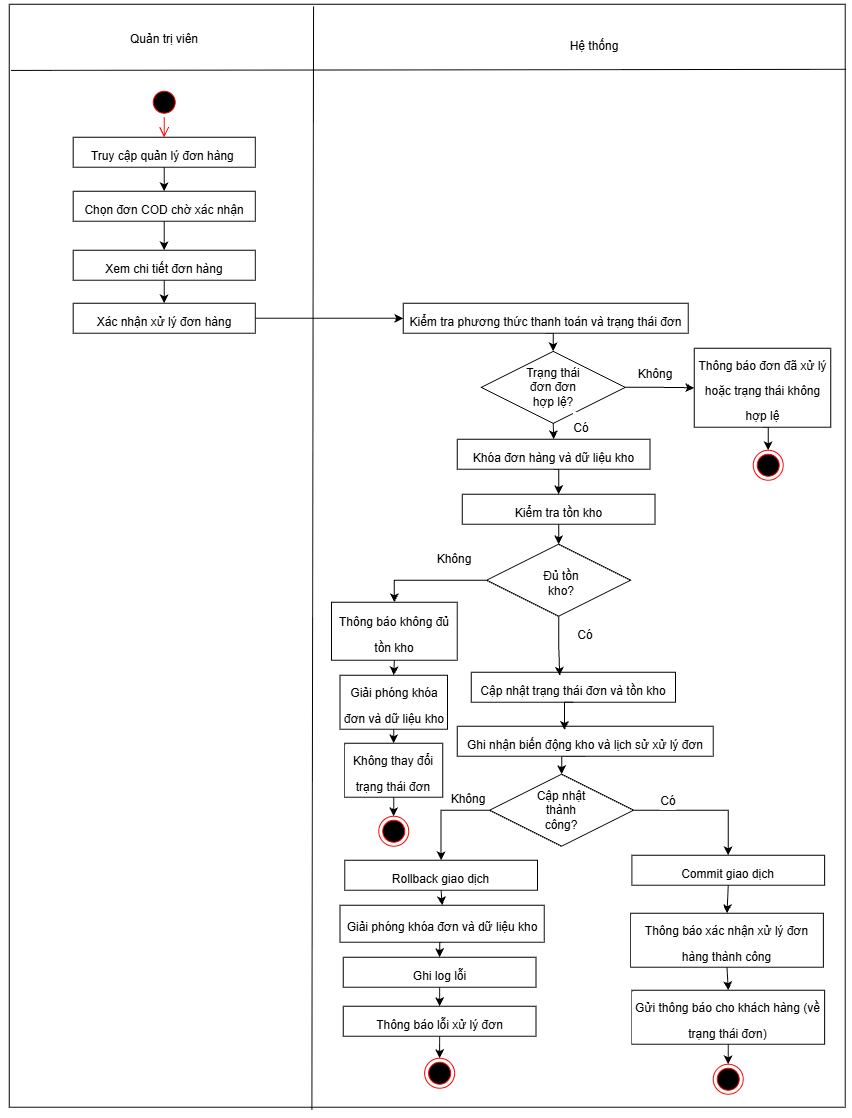
\includegraphics[width=\linewidth,height=0.82\textheight,keepaspectratio]{Images/Activity/da-Xử lý và xác nhận đơn COD.drawio.png}
    \caption{Activity Diagram xử lý và xác nhận đơn COD}
    \label{fig:activity-cod-confirmation}
\end{figure}

Cơ chế khóa và giao dịch bảo đảm hai quản trị viên không đồng thời xác nhận cùng một đơn, đồng thời ngăn trạng thái đơn và số lượng tồn kho bị cập nhật không nhất quán.

\subsubsection{Hoạt động tìm kiếm sản phẩm đa phương thức}

Hình~\ref{fig:activity-multimodal-search} tổng hợp UC-AI-01, UC-AI-02, UC-AI-03 và UC-AI-05. Dựa trên đầu vào, AI Service định tuyến sang tìm kiếm văn bản, hình ảnh hoặc kết hợp. Nhánh văn bản phân tích ý định, trích xuất bộ lọc, tạo text embedding và truy xuất text collection. Nhánh hình ảnh kiểm tra ảnh, sử dụng vùng chọn hoặc ảnh gốc, tạo image embedding và truy xuất image collection.

Với tìm kiếm kết hợp, hai nhánh text và image được xử lý và truy xuất trên các collection tương ứng trước khi hợp nhất danh sách ứng viên. Hệ thống không fusion hai embedding trước khi truy vấn. Sau điểm hợp nhất, các kết quả được lọc theo metadata, rerank nếu tính năng này được bật, rồi đối chiếu với dữ liệu hiện hành từ MySQL để bổ sung giá, khuyến mãi và tồn kho trước khi hiển thị.

\begin{figure}[H]
    \centering
    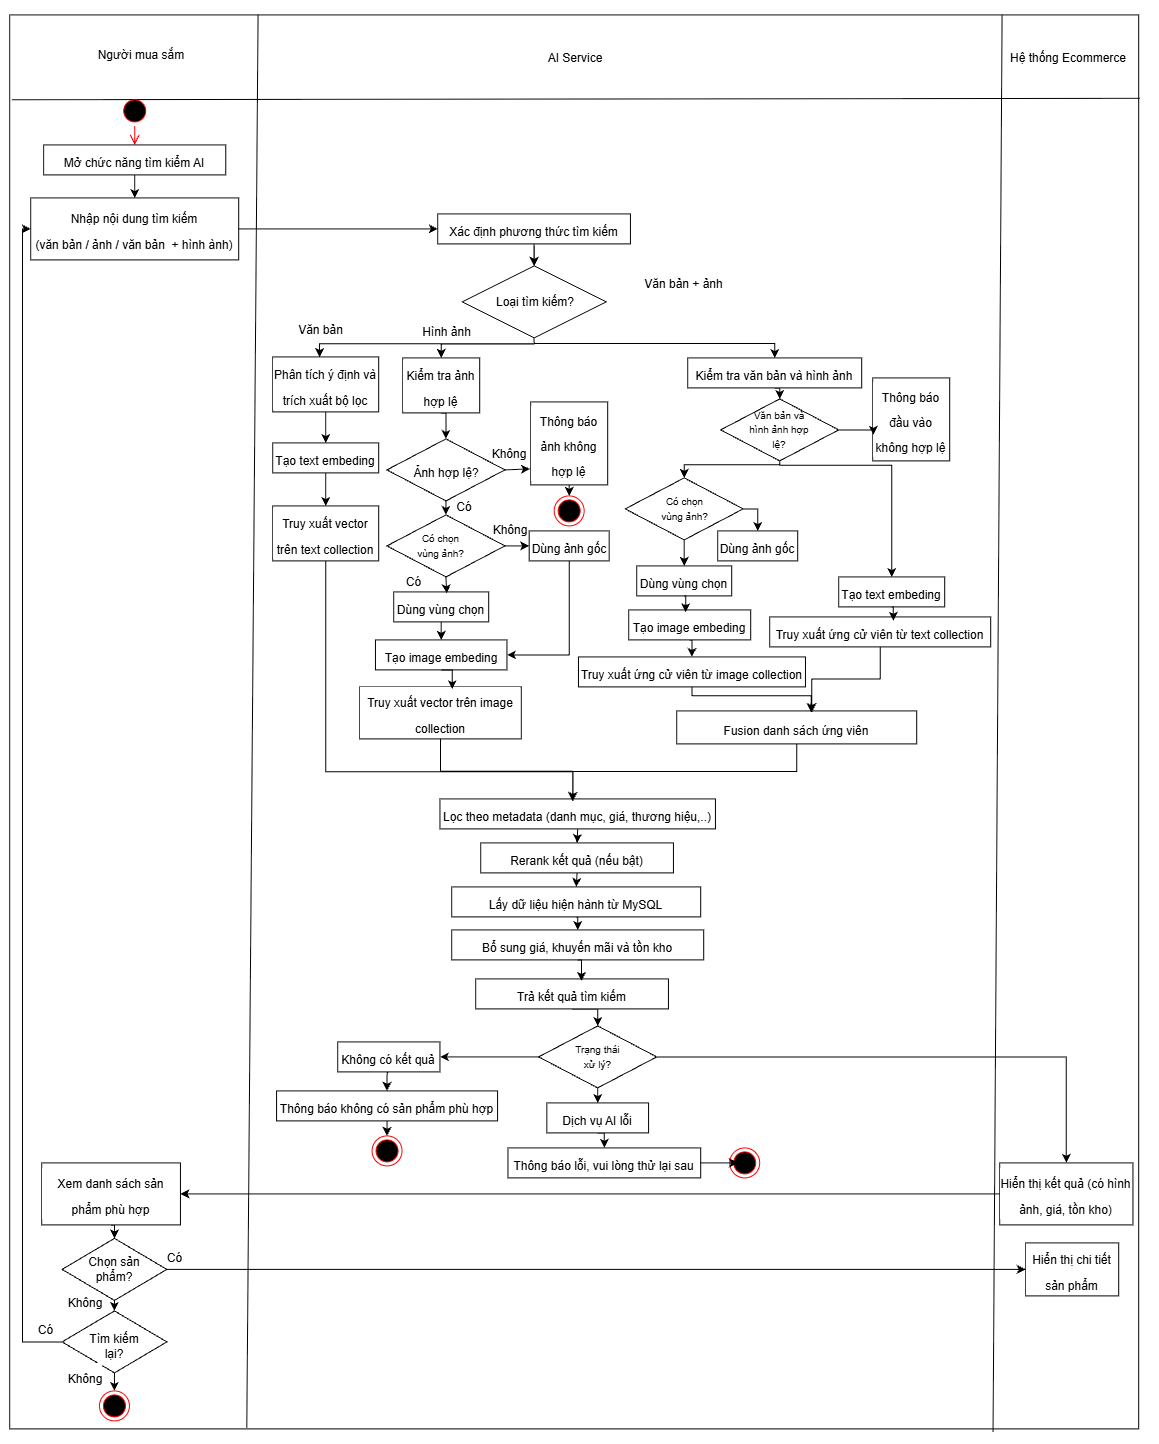
\includegraphics[width=\linewidth,height=0.84\textheight,keepaspectratio]{Images/Activity/da-Tìm kiếm sản phẩm đa phương thức.drawio.png}
    \caption{Activity Diagram tìm kiếm sản phẩm đa phương thức}
    \label{fig:activity-multimodal-search}
\end{figure}

Nếu không có sản phẩm phù hợp, hệ thống trả trạng thái không có kết quả; nếu AI Service gặp lỗi, người dùng nhận thông báo để thử lại. Ở luồng thành công, người dùng có thể xem chi tiết một sản phẩm, thực hiện truy vấn mới hoặc kết thúc phiên tìm kiếm.

\subsubsection{Hoạt động chat tư vấn sản phẩm đa lượt}

Hình~\ref{fig:activity-multiturn-chat} mô tả UC-AI-04 và nhánh phản hồi UC-AI-06. Hệ thống tạo hoặc khôi phục phiên hội thoại, kiểm tra đầu vào rồi chuyển yêu cầu cùng ngữ cảnh đến AI Service. AI Service đọc conversation memory và phân loại ý định thành tìm kiếm sản phẩm, thay đổi điều kiện, hỏi thông tin, small-talk hoặc yêu cầu ngoài phạm vi. Các ý định cần dữ liệu sản phẩm được đưa qua retrieval, lọc metadata và đối chiếu giá, tồn kho hiện hành trước khi tạo câu trả lời có căn cứ.

\begin{figure}[H]
    \centering
    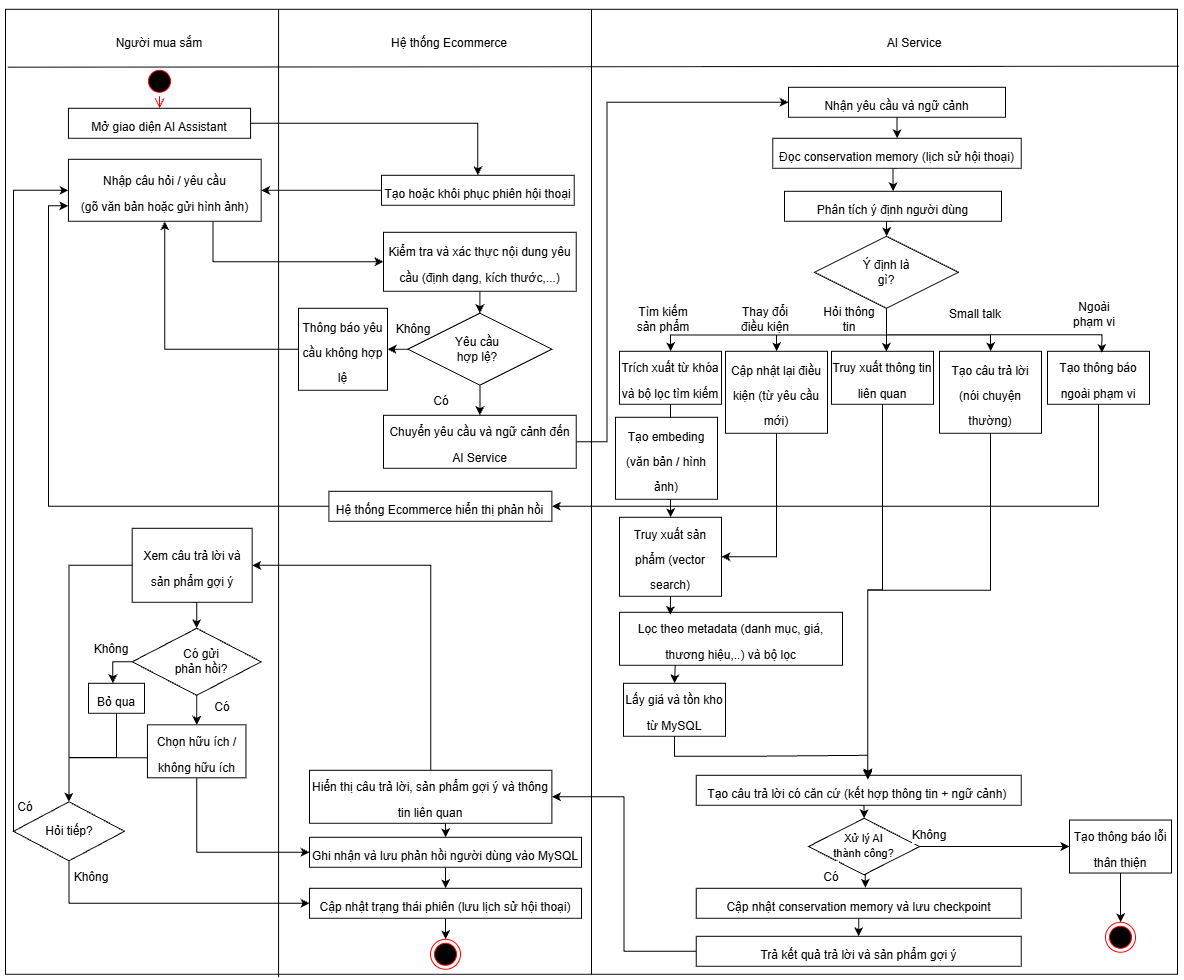
\includegraphics[width=\linewidth,height=0.78\textheight,keepaspectratio]{Images/Activity/da-Chat tư vấn sản phẩm đa lượt.drawio.png}
    \caption{Activity Diagram chat tư vấn sản phẩm đa lượt}
    \label{fig:activity-multiturn-chat}
\end{figure}

Sau mỗi lượt thành công, AI Service cập nhật conversation memory và checkpoint. Người dùng có thể đánh giá câu trả lời là hữu ích hoặc không hữu ích, sau đó tiếp tục đặt câu hỏi trong cùng phiên. Khi người dùng không hỏi tiếp, hệ thống lưu trạng thái phiên và kết thúc; lỗi từ retrieval hoặc mô hình AI được chuyển thành thông báo thân thiện.

\subsubsection{Hoạt động đồng bộ chỉ mục AI}

Hình~\ref{fig:activity-ai-index-sync} mô tả UC-AD-11, UC-AD-12, UC-AI-07 và UC-AI-08. Quản trị viên có thể chọn đồng bộ toàn bộ, tăng dần, theo giới hạn hoặc theo mã sản phẩm. Backend nghiệp vụ kiểm tra quyền và tham số, tạo tác vụ ở trạng thái \texttt{QUEUED}, sau đó chuyển sang \texttt{RUNNING}, lấy dữ liệu từ MySQL và chia danh sách sản phẩm thành các batch.

\begin{figure}[H]
    \centering
    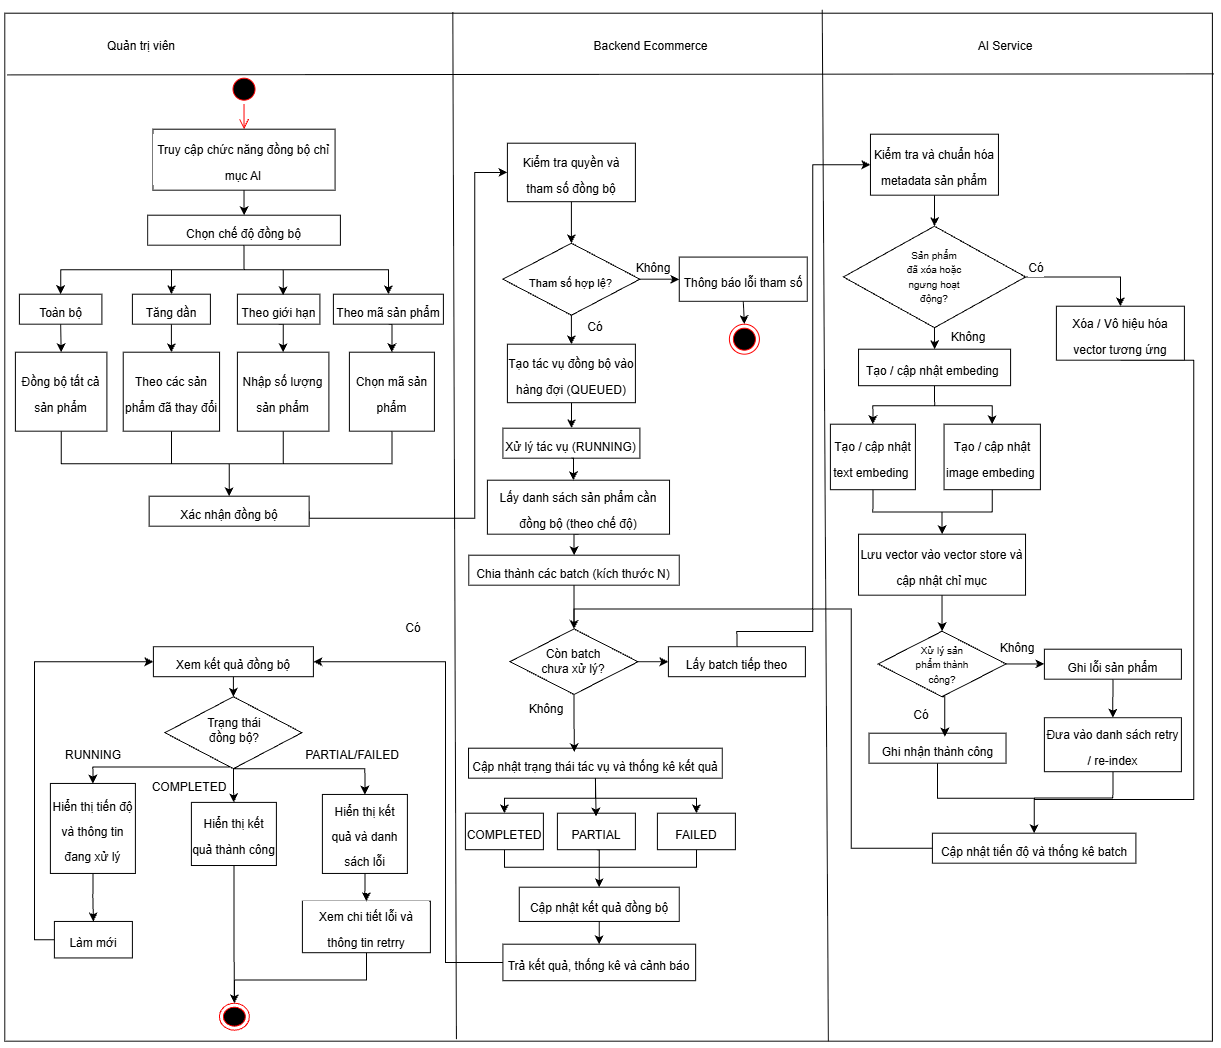
\includegraphics[width=\linewidth,height=0.80\textheight,keepaspectratio]{Images/Activity/da-Đồng bộ chỉ mục AI.drawio.png}
    \caption{Activity Diagram đồng bộ chỉ mục AI}
    \label{fig:activity-ai-index-sync}
\end{figure}

AI Service chuẩn hóa metadata, tạo hoặc cập nhật text embedding và image embedding, rồi lưu vector cùng payload vào vector store. Với sản phẩm đã xóa hoặc ngừng hoạt động, vector tương ứng được xóa hoặc vô hiệu hóa. Kết quả của từng batch được ghi nhận để cập nhật tiến độ; sản phẩm lỗi được đưa vào danh sách retry/re-index mà không làm dừng toàn bộ tác vụ. Khi không còn batch, Backend nghiệp vụ tổng hợp trạng thái \texttt{COMPLETED}, \texttt{PARTIAL} hoặc \texttt{FAILED} và trả thống kê, cảnh báo cho quản trị viên.

\FloatBarrier
\subsection*{Kết chương}

Chương này đã phân tích hệ thống ở các góc nhìn bổ trợ nhau. Ba nhóm Use Case và các bảng đặc tả xác định chức năng, tác nhân, điều kiện và ngoại lệ; năm Activity Diagram mô tả luồng điều khiển, các điểm quyết định và trách nhiệm của những thành phần tham gia các nghiệp vụ tiêu biểu.

Kết quả phân tích bao quát quy trình đặt và xác nhận đơn COD, tìm kiếm đa phương thức, hội thoại tư vấn nhiều lượt và đồng bộ chỉ mục AI. Đây là cơ sở để thiết kế kiến trúc, dữ liệu, giao tiếp dịch vụ và AI retrieval pipeline ở chương tiếp theo.

% Sections/07-ThietKeHeThong.tex
% Chương 6 -- Thiết kế hệ thống
%=========================

\section{Thiết kế hệ thống}

Chương này chuyển các yêu cầu và quy trình đã phân tích ở chương trước thành thiết kế kỹ thuật cho hệ thống thương mại điện tử tích hợp AI Shopping Assistant. Nội dung tập trung vào cấu trúc thành phần, dữ liệu, giao tiếp, bảo mật và triển khai; các mô tả nghiệp vụ chi tiết không được lặp lại. Spring Boot Backend là cổng giao tiếp duy nhất của Frontend, còn MySQL là nguồn dữ liệu nghiệp vụ chính. AI Service hỗ trợ truy hồi và tư vấn nhưng không thay thế Backend trong việc xác nhận sản phẩm, giá, tồn kho và đơn hàng.

\subsection{Tổng quan thiết kế hệ thống}

\subsubsection{Phạm vi và ranh giới hệ thống}

Hệ thống được thiết kế cho hai nhóm tác nhân chính là khách hàng và quản trị viên. Khách hàng sử dụng các chức năng duyệt sản phẩm, tìm kiếm, trợ lý hội thoại, giỏ hàng và đặt hàng; quản trị viên vận hành catalog, tồn kho, đơn hàng, nội dung và quá trình đồng bộ chỉ mục AI. Trong phạm vi hiện tại, quy trình thanh toán được thiết kế cho phương thức thanh toán khi nhận hàng (COD); các cổng thanh toán trực tuyến không thuộc phạm vi triển khai.

Ranh giới hệ thống bao gồm Frontend, Spring Boot Backend, AI Service và các kho dữ liệu do ứng dụng quản lý. Trình duyệt chỉ gửi request đến Spring Boot Backend. Các nhà cung cấp mô hình, dịch vụ lưu trữ ảnh và hạ tầng triển khai được xem là hệ thống bên ngoài được truy cập thông qua adapter hoặc giao diện tích hợp. Cách xác định ranh giới này giúp tránh để client truy cập trực tiếp khóa mô hình, chỉ mục vector hoặc cơ sở dữ liệu nghiệp vụ.

\subsubsection{Mục tiêu và nguyên tắc thiết kế}

Thiết kế hệ thống hướng đến các mục tiêu sau:

\begin{itemize}
    \item Tách biệt nghiệp vụ thương mại điện tử khỏi các tác vụ AI để hai khối có thể phát triển và triển khai độc lập.
    \item Chỉ cho phép Frontend giao tiếp với Spring Boot Backend; AI Service được sử dụng như một dịch vụ nội bộ.
    \item Xem MySQL là nguồn dữ liệu chuẩn và Qdrant là chỉ mục phục vụ truy hồi có thể tái tạo.
    \item Hỗ trợ tìm kiếm bằng văn bản, hình ảnh, tìm kiếm kết hợp và hội thoại nhiều lượt.
    \item Lựa chọn LLM, embedding và reranker qua cấu hình thay vì gắn kiến trúc với một mô hình cụ thể.
    \item Cô lập lỗi AI khỏi giỏ hàng, đặt hàng, thanh toán và quản lý tồn kho.
\end{itemize}

Mỗi thành phần chỉ nắm giữ trách nhiệm thuộc phạm vi của mình. Mọi kết quả AI chứa mã sản phẩm phải được Backend đối chiếu lại với MySQL trước khi trả cho người dùng. Các tích hợp bên ngoài phải có timeout, kiểm tra lỗi và phương án dự phòng.

% \subsubsection{Các quyết định kiến trúc từ yêu cầu phi chức năng}

% Các quyết định thiết kế tổng quát được xây dựng từ nhóm yêu cầu phi chức năng ở Chương 5. Bảng~\ref{tab:overview-architecture-decisions} trình bày quan hệ giữa yêu cầu và giải pháp kiến trúc được lựa chọn.

% \begin{table}[H]
% \centering
% \caption{Ánh xạ yêu cầu phi chức năng với quyết định kiến trúc}
% \label{tab:overview-architecture-decisions}
% \begin{tabularx}{\linewidth}{@{}p{0.15\linewidth}p{0.23\linewidth}X@{}}
% \toprule
% \textbf{Yêu cầu} & \textbf{Thuộc tính} & \textbf{Quyết định thiết kế} \\
% \midrule
% NFR-01 & Hiệu năng & Giới hạn số kết quả, cấu hình timeout và tách các bước phân tích, embedding, retrieval, rerank để có thể đo thời gian từng bước. \\
% NFR-02 & Bảo mật & Sử dụng JWT, phân quyền theo vai trò, khóa API nội bộ và giới hạn truy cập MySQL, Qdrant trong mạng dịch vụ. \\
% NFR-03, NFR-04 & Khả dụng và tin cậy & Tách AI Service khỏi nghiệp vụ cốt lõi; MySQL giữ dữ liệu giao dịch và lỗi AI không làm mất hoặc sửa sai đơn hàng. \\
% NFR-05 & Bảo trì, mở rộng & Module hóa frontend, backend và AI Service; dùng adapter và biến môi trường để thay provider hoặc mô hình. \\
% NFR-06 & Tương thích & Frontend đáp ứng nhiều kích thước màn hình; các dịch vụ trao đổi dữ liệu JSON qua HTTP. \\
% NFR-07 & Khả năng quan sát & Cung cấp health check, metrics và log theo mã tương quan nhưng không ghi dữ liệu nhạy cảm. \\
% NFR-08 & Nhất quán & MySQL là nguồn chuẩn; Qdrant là chỉ mục có thể tái tạo; checkpoint hội thoại không thay thế dữ liệu giao dịch. \\
% NFR-09 & Tài nguyên AI & Ưu tiên provider được quản lý; embedding, reranker và phát hiện vật thể được bật, tắt hoặc thay thế qua cấu hình. \\
% \bottomrule
% \end{tabularx}
% \end{table}

\subsubsection{Kiến trúc tổng thể}

Hệ thống gồm Frontend React được phục vụ qua nginx, Spring Boot Backend, AI Service FastAPI, MySQL, Qdrant, kho checkpoint hội thoại, dịch vụ lưu trữ ảnh và các dịch vụ mô hình. Frontend cung cấp giao diện mua sắm và trợ lý; Spring Boot xử lý xác thực cùng toàn bộ nghiệp vụ; AI Service phân tích truy vấn, tạo embedding, truy hồi và điều phối hội thoại; MySQL lưu dữ liệu giao dịch; Qdrant lưu vector cùng metadata phục vụ tìm kiếm.

Trạng thái hội thoại được lưu qua checkpointer có Backend lựa chọn bằng cấu hình. SQLite phù hợp với môi trường đơn instance và kiểm thử; PostgreSQL hoặc Redis có thể được sử dụng khi cần chia sẻ trạng thái giữa nhiều instance. Ảnh sản phẩm được quản lý bằng URL và dịch vụ lưu trữ ảnh, trong khi health check, log và metrics cung cấp dữ liệu quan sát cho các thành phần vận hành. Các thành phần lưu trữ và giám sát này hỗ trợ hệ thống nhưng không nắm quyền quyết định đối với giao dịch thương mại điện tử.

\begin{figure}[H]
    \centering
    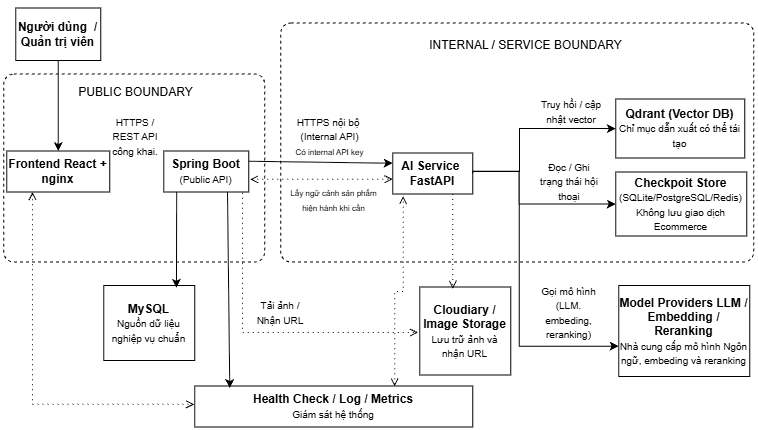
\includegraphics[width=0.98\textwidth]{Images/Thietkehethong/Kiến trúc tổng thể của hệ thống.drawio.drawio.png}
    \caption{Kiến trúc tổng thể của hệ thống}
    \label{fig:system-architecture}
\end{figure}

Hình~\ref{fig:system-architecture} phân chia hệ thống thành vùng truy cập công khai, vùng dịch vụ nội bộ và nhóm dịch vụ tích hợp bên ngoài. Người dùng và quản trị viên tương tác với Frontend React được phục vụ qua nginx. Frontend trao đổi với Spring Boot qua REST API công khai; Frontend không gọi trực tiếp AI Service hoặc các kho dữ liệu. Spring Boot vừa là cổng vào của hệ thống, vừa là thành phần điều phối nghiệp vụ và kiểm soát dữ liệu trả về client.

Trong vùng dịch vụ nội bộ, Spring Boot truy cập MySQL để xử lý dữ liệu nghiệp vụ và gọi AI Service FastAPI qua API nội bộ có khóa xác thực. AI Service truy vấn hoặc cập nhật vector trong Qdrant, đồng thời đọc và ghi checkpoint phục vụ hội thoại nhiều lượt. Khi cần phân tích truy vấn, sinh embedding, rerank hoặc tạo câu trả lời, AI Service gọi nhà cung cấp mô hình thông qua adapter tương ứng. Chiều gọi ngược từ AI Service về Spring Boot chỉ được sử dụng để lấy ngữ cảnh sản phẩm hiện hành khi cần; AI Service không truy cập trực tiếp MySQL.

Cloudinary hoặc dịch vụ lưu trữ ảnh tiếp nhận tệp từ Backend và trả URL để lưu cùng dữ liệu catalog. AI Service có thể tải ảnh thông qua URL cho quá trình lập chỉ mục hoặc tìm kiếm ảnh. Các thành phần Frontend, Spring Boot và AI Service đồng thời phát sinh health check, log và metrics để theo dõi trạng thái, độ trễ và lỗi. Cách bố trí này tạo ranh giới rõ giữa dữ liệu giao dịch, dữ liệu dẫn xuất và dịch vụ AI, qua đó hạn chế sự cố ở một thành phần lan sang toàn bộ hệ thống.

\subsubsection{Quyền sở hữu và vòng đời dữ liệu}

Mỗi kho dữ liệu được sử dụng cho một mục đích riêng. Việc xác định nguồn dữ liệu chuẩn giúp hệ thống xử lý đúng khi thông tin trong các kho tạm thời chưa đồng bộ.

\begin{table}[H]
\centering
\caption{Vai trò và quyền sở hữu dữ liệu của các kho lưu trữ}
\label{tab:overview-data-ownership}
\begin{tabularx}{\linewidth}{|p{0.20\linewidth}|p{0.41\linewidth}|X|}
\hline
\textbf{Kho dữ liệu} & \textbf{Vai trò} & \textbf{Nguyên tắc sử dụng} \\ \hline
MySQL & Lưu tài khoản, catalog, giá, tồn kho, giỏ hàng, đơn hàng và thanh toán. & Là nguồn dữ liệu nghiệp vụ chuẩn và được bảo vệ bằng giao dịch. \\ \hline
Qdrant & Lưu vector văn bản, vector hình ảnh và metadata truy hồi. & Là chỉ mục dẫn xuất; có thể tái tạo từ dữ liệu sản phẩm và không quyết định dữ liệu hiển thị cuối cùng. \\ \hline
Kho checkpoint & Lưu trạng thái workflow, tóm tắt, ràng buộc và lựa chọn theo phiên hội thoại. & Có thể dùng SQLite, PostgreSQL hoặc Redis theo môi trường; không lưu giao dịch thương mại điện tử. \\ \hline
Dịch vụ lưu trữ ảnh & Lưu tệp ảnh và cung cấp URL cho catalog hoặc truy vấn ảnh. & Backend kiểm tra tệp và chỉ lưu URL cần thiết trong dữ liệu sản phẩm. \\ \hline
Log và metrics & Lưu thông tin lỗi, latency và trạng thái vận hành. & Chỉ phục vụ quan sát, không chứa token, bí mật hoặc nội dung nhạy cảm không cần thiết. \\ \hline
\end{tabularx}
\end{table}

\subsubsection{Luồng xử lý tổng quát}

Hệ thống có ba luồng xử lý tổng quát. Thứ nhất, luồng thương mại điện tử đi từ Frontend đến Spring Boot, thực hiện kiểm tra quyền và nghiệp vụ, truy cập MySQL rồi trả response cho Frontend. Luồng này không phụ thuộc vào Qdrant hoặc nhà cung cấp mô hình.

Thứ hai, luồng AI trực tuyến bắt đầu khi Frontend gửi truy vấn văn bản, ảnh hoặc hội thoại đến Spring Boot. Backend xác thực và chuyển dữ liệu cần thiết sang AI Service. AI Service đọc checkpoint khi có phiên hội thoại, phân tích truy vấn, tạo embedding, truy hồi Qdrant và có thể gọi mô hình để tạo phản hồi. Danh sách mã sản phẩm được trả về Spring Boot để đối chiếu lại với MySQL trước khi gửi kết quả cuối cùng đến Frontend.

Thứ ba, luồng đồng bộ chỉ mục được kích hoạt bởi quản trị viên hoặc tác vụ hệ thống. Spring Boot đọc sản phẩm từ MySQL, chuẩn hóa dữ liệu và gửi theo batch đến AI Service. AI Service tạo embedding rồi thêm, cập nhật hoặc xóa vector trong Qdrant. Lỗi đồng bộ được ghi nhận để thử lại nhưng không hoàn tác dữ liệu nghiệp vụ đã lưu thành công trong MySQL.

Ba luồng trên sử dụng chung nguyên tắc: Spring Boot kiểm soát ranh giới công khai, dữ liệu giao dịch chỉ được ghi tại MySQL, còn các thành phần AI có thể suy giảm độc lập. Vì vậy, khi AI Service, Qdrant hoặc nhà cung cấp mô hình tạm thời không khả dụng, người dùng vẫn có thể duyệt catalog, quản lý giỏ hàng và thực hiện các nghiệp vụ thương mại điện tử còn lại.

\subsection{Thiết kế kiến trúc}

\subsubsection{Kiến trúc phía máy khách}

Frontend được xây dựng dưới dạng ứng dụng trang đơn bằng React. Mã nguồn được chia thành các nhóm \texttt{Pages}, \texttt{Layouts}, \texttt{components}, \texttt{Route}, \texttt{redux}, \texttt{api} và các tiện ích dùng chung. Cách tổ chức này tách màn hình nghiệp vụ khỏi thành phần trình bày có thể tái sử dụng, đồng thời tập trung việc định tuyến, quản lý trạng thái và giao tiếp HTTP vào các mô-đun riêng.

Các trang và layout chịu trách nhiệm ghép thành phần giao diện theo từng luồng sử dụng. React Router ánh xạ URL đến trang tương ứng; \texttt{PrivateRoute} kiểm tra trạng thái đăng nhập trước khi hiển thị các màn hình được bảo vệ. Việc kiểm tra này chỉ phục vụ trải nghiệm phía máy khách, còn quyền truy cập thực sự vẫn được Spring Security xác minh tại Backend, vì trạng thái trên trình duyệt có thể bị thay đổi bởi người dùng.

Trạng thái dùng chung được quản lý bằng Redux. Một số dữ liệu phục vụ tính liên tục của giao diện được lưu cục bộ, chẳng hạn trạng thái đăng nhập và giỏ hàng trong \texttt{localStorage}, mã phiên trợ lý trong \texttt{sessionStorage}. Đây không phải nguồn dữ liệu nghiệp vụ chuẩn: giá bán, tồn kho, trạng thái đơn hàng và quyền người dùng luôn phải được đối chiếu lại qua API trước khi thực hiện thao tác có ảnh hưởng đến hệ thống.

Lớp \texttt{api} tập trung các lời gọi HTTP thông qua một Axios instance dùng chung. Interceptor gắn access token vào request và xử lý trạng thái hết phiên theo một quy tắc thống nhất. Các chức năng tìm kiếm văn bản, tìm kiếm ảnh, tìm kiếm lai và trợ lý hội thoại được khai báo tại \texttt{aiApi}, nhưng tất cả đều gọi endpoint của Spring Boot. Vì vậy Frontend không giữ khóa truy cập AI, không kết nối trực tiếp AI Service, MySQL hoặc Qdrant và không tự quyết định kết quả nghiệp vụ.

\begin{table}[H]
    \centering
    \caption{Các nhóm thành phần chính của Frontend}
    \label{tab:frontend-components}
    \begin{tabularx}{\textwidth}{|p{0.23\textwidth}|X|}
        \hline
        \textbf{Nhóm thành phần} & \textbf{Trách nhiệm} \\
        \hline
        Trang và bố cục & Tổ chức màn hình theo luồng nghiệp vụ và xác định cấu trúc hiển thị chung. \\
        \hline
        Thành phần giao diện & Đóng gói các phần tử có thể tái sử dụng, tiếp nhận dữ liệu qua thuộc tính và phát sinh sự kiện người dùng. \\
        \hline
        Định tuyến & Ánh xạ URL đến màn hình, điều hướng và kiểm tra điều kiện hiển thị các tuyến riêng tư. \\
        \hline
        Redux và lưu trữ cục bộ & Quản lý trạng thái dùng chung và duy trì một số trạng thái giao diện qua lần tải lại trang. \\
        \hline
        API và tiện ích & Chuẩn hóa URL, header xác thực, cách gửi request, xử lý lỗi và chuyển đổi dữ liệu phục vụ giao diện. \\
        \hline
    \end{tabularx}
\end{table}

\subsubsection{Kiến trúc Spring Boot Backend}

Backend được tổ chức theo kiến trúc phân lớp để tách giao tiếp HTTP, quy tắc nghiệp vụ, truy cập dữ liệu và tích hợp bên ngoài. Mỗi lớp chỉ phụ thuộc vào giao diện của lớp kế tiếp, nhờ đó thay đổi ở cơ sở dữ liệu hoặc AI Service không buộc Frontend thay đổi theo.

\begin{figure}[H]
    \centering
    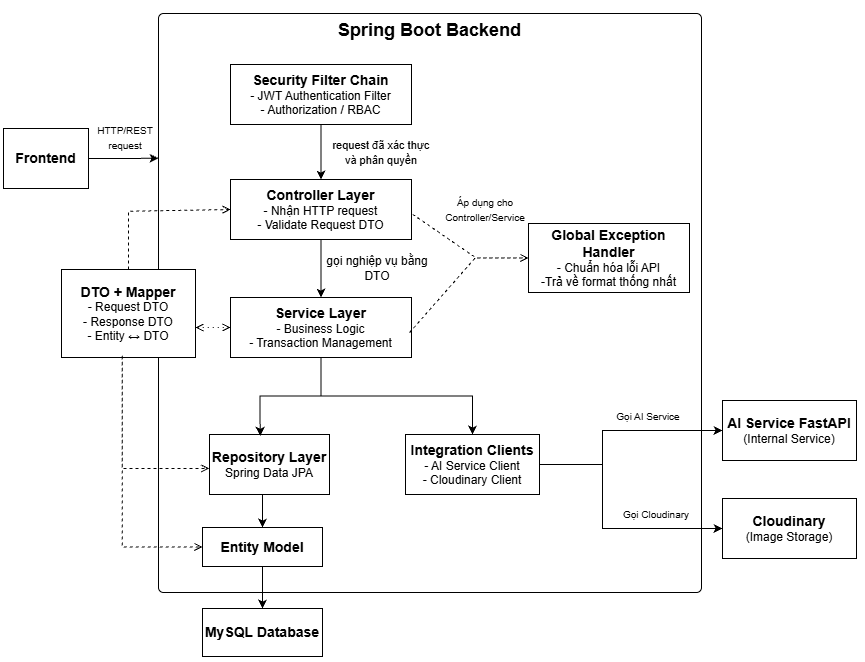
\includegraphics[width=0.98\textwidth]{Images/Thietkehethong/Kiến trúc phân lớp của Spring Boot Backend.drawio.png}
    \caption{Kiến trúc phân lớp của Spring Boot Backend}
    \label{fig:backend-layers}
\end{figure}

Như trình bày tại Hình~\ref{fig:backend-layers}, request từ Frontend trước hết đi qua Security Filter Chain. JWT Authentication Filter đọc và kiểm tra access token, sau đó thiết lập thông tin xác thực cho request. Cấu hình phân quyền quyết định endpoint nào được truy cập công khai, endpoint nào yêu cầu đăng nhập và nhóm \texttt{/admin} nào yêu cầu vai trò quản trị. Khi xác thực hoặc phân quyền thất bại, \texttt{AuthenticationEntryPoint} và \texttt{AccessDeniedHandler} lần lượt chuẩn hóa phản hồi HTTP 401 và 403.

Sau lớp bảo mật, Controller tiếp nhận request, ánh xạ tham số và kiểm tra Request DTO. Controller không chứa quy tắc nghiệp vụ phức tạp mà chuyển dữ liệu hợp lệ xuống Service. Service là lớp trung tâm thực hiện nghiệp vụ, kiểm tra các ràng buộc liên miền và xác định phạm vi giao dịch. Những thao tác cần cập nhật nhất quán nhiều bảng, chẳng hạn tạo đơn hàng, giữ tồn kho hoặc ghi nhận thanh toán, được quản lý transaction tại lớp này.

Repository sử dụng Spring Data JPA để thao tác với MySQL thông qua các Entity ánh xạ bảng. MySQL nằm ngoài tiến trình Spring Boot và là nguồn dữ liệu nghiệp vụ chuẩn. DTO được dùng tại ranh giới API, còn Mapper chuyển đổi giữa DTO và Entity; do đó cấu trúc bảng không bị để lộ trực tiếp cho Frontend và thay đổi response không nhất thiết làm thay đổi mô hình lưu trữ.

Các kết nối ra ngoài được đóng gói trong Integration Clients. AI Service Client chuyển các yêu cầu tìm kiếm, hội thoại và đồng bộ chỉ mục đến AI Service FastAPI; Cloudinary Client thực hiện tải ảnh và nhận URL lưu trữ. Cách đóng gói này tập trung cấu hình URL, xác thực, timeout và xử lý lỗi của từng dịch vụ. Ngoại lệ phát sinh từ Controller hoặc Service được Global Exception Handler chuyển thành cấu trúc lỗi API thống nhất, trong khi chi tiết kỹ thuật chỉ được ghi trong log của Backend.

\subsubsection{Kiến trúc AI Service}

AI Service được triển khai bằng FastAPI và tổ chức theo hướng mô-đun. Tầng \texttt{api/routes} công bố các endpoint tìm kiếm, trợ lý, đồng bộ chỉ mục, kiểm tra trạng thái và số liệu vận hành; các schema định nghĩa cấu trúc request và response tại ranh giới dịch vụ. Route chỉ xác thực dữ liệu đầu vào và chuyển yêu cầu đến lớp dịch vụ, không chứa chi tiết của mô hình AI hay kho vector.

Lớp dịch vụ gồm các mô-đun \texttt{search}, \texttt{embeddings}, \texttt{cropping}, \texttt{query\_understanding}, \texttt{reranking}, \texttt{assistant} và \texttt{indexing}. Mỗi mô-đun đảm nhiệm một bước độc lập trong chuỗi xử lý. Các adapter thuộc tầng \texttt{infrastructure} đóng gói kết nối đến Qdrant, Spring Boot và nhà cung cấp mô hình. Nhờ phụ thuộc vào giao diện chung thay vì một hiện thực cố định, hệ thống có thể lựa chọn nhà cung cấp LLM, embedding và reranking bằng cấu hình môi trường mà không phải thay đổi route nghiệp vụ.

Với yêu cầu tìm kiếm, dữ liệu đầu vào được chuẩn hóa và phân tích để nhận diện từ khóa hoặc bộ lọc có cấu trúc. Mô-đun embedding chuyển văn bản hay ảnh thành vector; Search Service truy vấn Qdrant để lấy tập ứng viên và có thể gọi reranker để sắp xếp lại. Kết quả trả về chỉ gồm định danh sản phẩm, điểm số và thông tin giải thích cần thiết. Spring Boot dùng các định danh này để lấy dữ liệu hiện hành từ MySQL, loại bỏ sản phẩm không còn hợp lệ và tạo response cuối cùng cho Frontend.

Đối với tìm kiếm ảnh, mô-đun cropping có thể sử dụng toàn bộ ảnh, vùng do người dùng chọn hoặc vùng đối tượng được YOLO phát hiện. YOLO là thành phần tùy chọn; khi bị tắt hoặc không tìm thấy đối tượng phù hợp, chuỗi xử lý vẫn tiếp tục bằng ảnh gốc. Thiết kế suy giảm này tránh biến mô-đun phát hiện đối tượng thành điểm lỗi bắt buộc của chức năng tìm kiếm ảnh.

Trợ lý hội thoại được tổ chức thành workflow có trạng thái. Workflow tiếp nhận câu hỏi và ngữ cảnh phiên, phân loại nhu cầu, gọi công cụ tìm kiếm hoặc API ngữ cảnh của Spring Boot khi cần, sau đó mới tạo câu trả lời. Checkpoint lưu trạng thái hội thoại theo phiên và có thể được cấu hình trên SQLite, PostgreSQL hoặc Redis. Dữ liệu checkpoint hỗ trợ tiếp tục hội thoại nhưng không thay thế hồ sơ người dùng hay dữ liệu giao dịch trong MySQL.

Luồng indexing nhận dữ liệu sản phẩm đã được Spring Boot chuẩn hóa, tạo các biểu diễn vector cần thiết và ghi hoặc cập nhật điểm tương ứng trong Qdrant. Vì Qdrant chỉ là chỉ mục dẫn xuất, toàn bộ chỉ mục có thể được xây dựng lại từ dữ liệu chuẩn khi thay đổi mô hình embedding, cấu trúc payload hoặc khi cần phục hồi. Các endpoint health, readiness và metrics cung cấp khả năng quan sát trạng thái phụ thuộc, thời gian xử lý và lỗi của các chuỗi AI.

\begin{table}[H]
    \centering
    \caption{Trách nhiệm các mô-đun chính của AI Service}
    \label{tab:ai-service-components}
    \begin{tabularx}{\textwidth}{|p{0.25\textwidth}|X|}
        \hline
        \textbf{Mô-đun} & \textbf{Trách nhiệm} \\
        \hline
        API và schema & Kiểm tra dữ liệu, công bố hợp đồng HTTP và chuyển yêu cầu đến dịch vụ phù hợp. \\
        \hline
        Query understanding & Chuẩn hóa truy vấn và trích xuất ý định, từ khóa hoặc bộ lọc tìm kiếm. \\
        \hline
        Embedding, cropping và reranking & Tiền xử lý dữ liệu đa phương thức, tạo vector và cải thiện thứ tự tập ứng viên. \\
        \hline
        Search Service & Điều phối chuỗi truy vấn Qdrant và trả về định danh cùng điểm số ứng viên. \\
        \hline
        Assistant workflow & Quản lý luồng hội thoại, sử dụng công cụ và lưu checkpoint của phiên. \\
        \hline
        Indexing Service & Chuyển dữ liệu sản phẩm chuẩn hóa thành payload và vector có thể tái tạo trong Qdrant. \\
        \hline
        Infrastructure adapters & Cô lập kết nối Qdrant, Spring Boot, kho checkpoint và các nhà cung cấp mô hình. \\
        \hline
    \end{tabularx}
\end{table}

\subsubsection{Giao tiếp và phân chia trách nhiệm}

Các thành phần giao tiếp theo nguyên tắc một cổng công khai. Frontend chỉ gọi API của Spring Boot bằng HTTPS và JSON; access token được gửi trong header xác thực đối với endpoint yêu cầu đăng nhập. Spring Boot xác thực người dùng, kiểm tra quyền, thực hiện nghiệp vụ và chỉ chuyển sang AI Service phần dữ liệu tối thiểu cần cho tác vụ AI. Trình duyệt vì vậy không cần biết địa chỉ nội bộ hoặc thông tin xác thực của AI Service.

Spring Boot gọi AI Service qua HTTP nội bộ với khóa API giữa dịch vụ, timeout hữu hạn và cấu trúc lỗi được chuẩn hóa. Các thao tác có thể được gọi lại, đặc biệt là cập nhật chỉ mục, cần mang định danh ổn định để tránh tạo bản ghi vector trùng lặp. Khi AI Service trả về danh sách ứng viên, Backend lấy lại dữ liệu từ MySQL theo định danh, bảo toàn thứ tự xếp hạng nếu còn hợp lệ, rồi áp dụng các điều kiện nghiệp vụ trước khi phản hồi cho Frontend.

Theo chiều ngược lại, AI Service chỉ được gọi một tập API ngữ cảnh giới hạn của Spring Boot, chẳng hạn thông tin sản phẩm cần cho trợ lý. AI Service không dùng tài khoản cơ sở dữ liệu và không truy cập trực tiếp MySQL. Ranh giới này giúp các quy tắc phân quyền, lọc dữ liệu nhạy cảm và kiểm soát phiên bản dữ liệu vẫn tập trung tại Backend.

\begin{table}[H]
    \centering
    \caption{Hợp đồng giao tiếp giữa các thành phần}
    \label{tab:service-communication-contracts}
    \begin{tabularx}{\textwidth}{|p{0.20\textwidth}|p{0.21\textwidth}|X|}
        \hline
        \textbf{Kênh giao tiếp} & \textbf{Cơ chế bảo vệ} & \textbf{Trách nhiệm và cách xử lý lỗi} \\
        \hline
        Frontend $\rightarrow$ Spring Boot & HTTPS, JWT và kiểm tra quyền tại Backend & Spring Boot xác thực request, trả mã lỗi API thống nhất; Frontend chỉ hiển thị trạng thái và yêu cầu người dùng thao tác lại khi cần. \\
        \hline
        Spring Boot $\rightarrow$ AI Service & Mạng nội bộ, khóa API dịch vụ và timeout & Backend gửi dữ liệu tối thiểu, kiểm tra response và chuyển lỗi phụ thuộc thành phản hồi phù hợp; nghiệp vụ thương mại điện tử không phụ thuộc AI vẫn tiếp tục hoạt động. \\
        \hline
        AI Service $\rightarrow$ Spring Boot & API ngữ cảnh giới hạn và xác thực dịch vụ & AI Service chỉ đọc ngữ cảnh được cấp phép, không truy cập MySQL; khi thiếu ngữ cảnh, workflow trả kết quả suy giảm thay vì tự suy đoán dữ liệu giao dịch. \\
        \hline
    \end{tabularx}
\end{table}

\subsection{Thiết kế dữ liệu}

\subsubsection{Mô hình dữ liệu tổng quan}

Dữ liệu MySQL được phân chia thành các miền nghiệp vụ nhằm giới hạn trách nhiệm
của từng nhóm bảng và thuận lợi cho việc bảo trì. Sơ đồ tổng quan thể hiện các
bảng, khóa chính, khóa ngoại quan trọng và quan hệ giữa các miền; thuộc tính chi
tiết của từng bảng được trình bày trong các sơ đồ thành phần ở phần tiếp theo.

\begin{figure}[H]
    \centering
    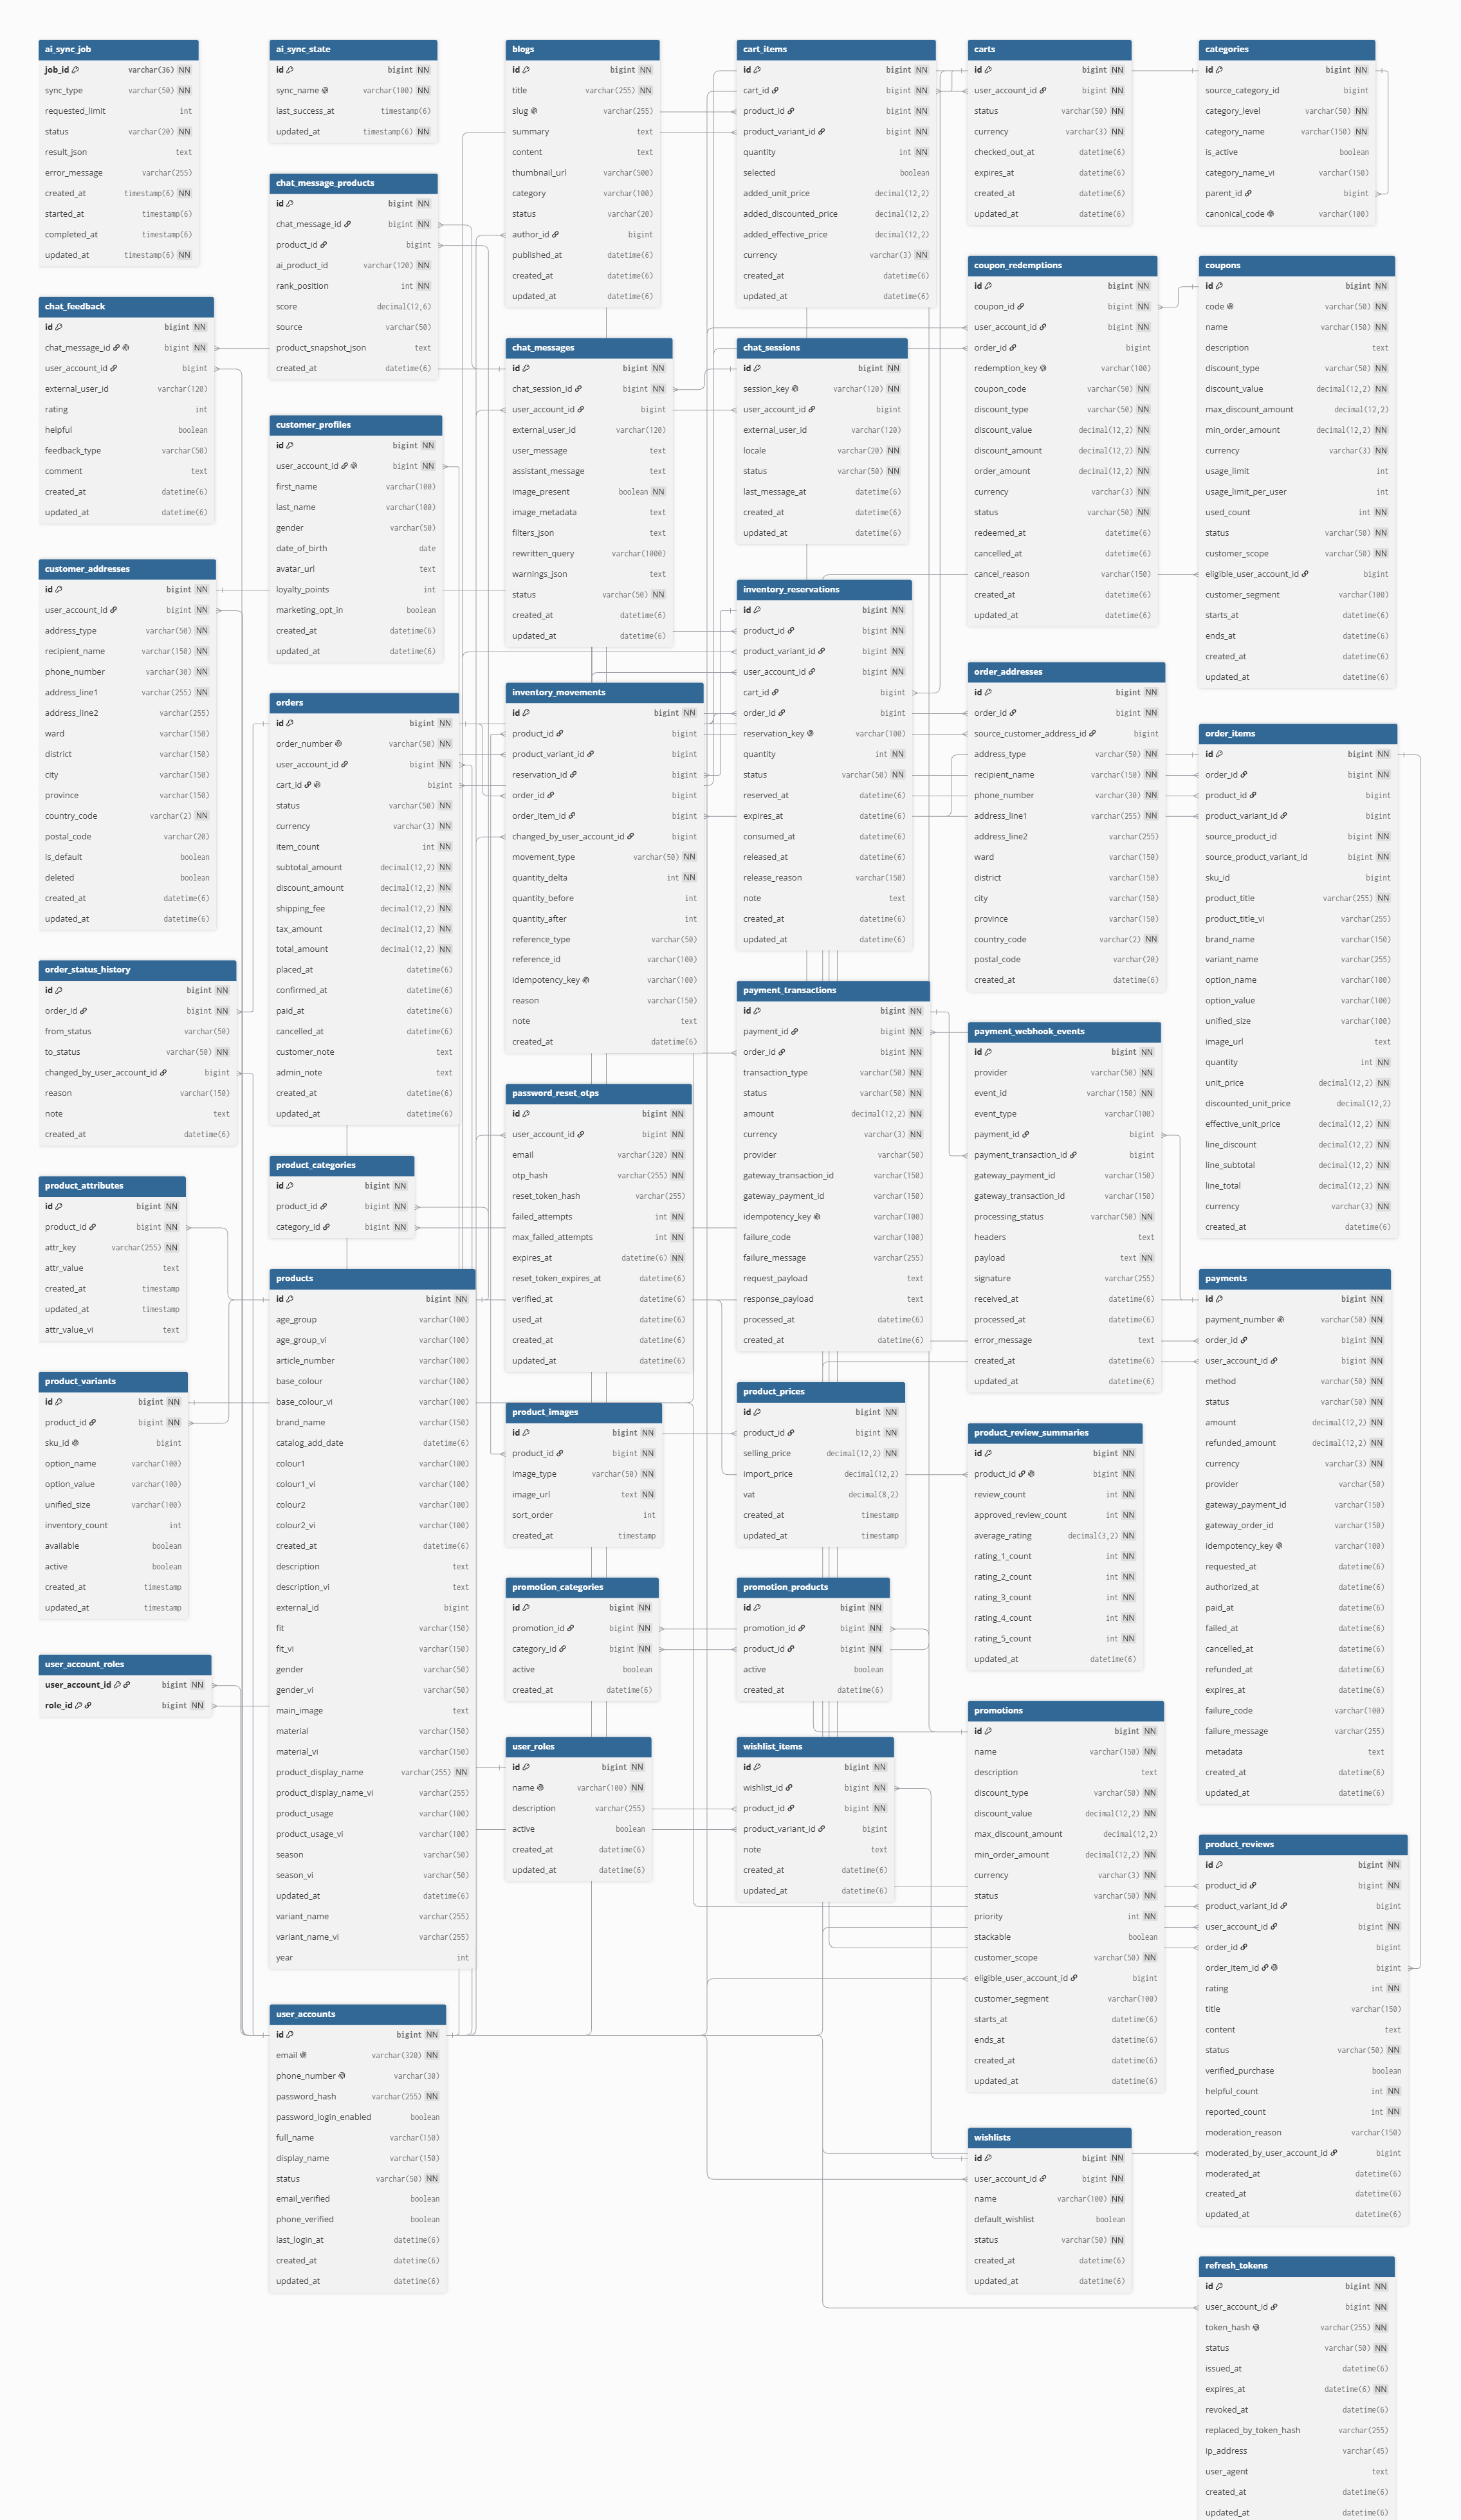
\includegraphics[
        width=\textwidth,
        height=0.82\textheight,
        keepaspectratio
    ]{Images/Thietkehethong/sơ đồ tổng quan toàn bộ cơ sở dữ liệu.png}
    \caption{Sơ đồ tổng quan toàn bộ cơ sở dữ liệu}
    \label{fig:database-overview}
\end{figure}

\subsubsection{Nhóm dữ liệu người dùng và phân quyền}

Nhóm này quản lý thông tin đăng nhập, hồ sơ, địa chỉ, vai trò và vòng đời thông
tin xác thực của người dùng. Quan hệ nhiều--nhiều giữa tài khoản và vai trò được
cài đặt qua bảng liên kết; refresh token và mã OTP khôi phục mật khẩu được lưu
riêng để có thể thu hồi, giới hạn thời gian sử dụng và truy vết độc lập.

\begin{figure}[H]
    \centering
    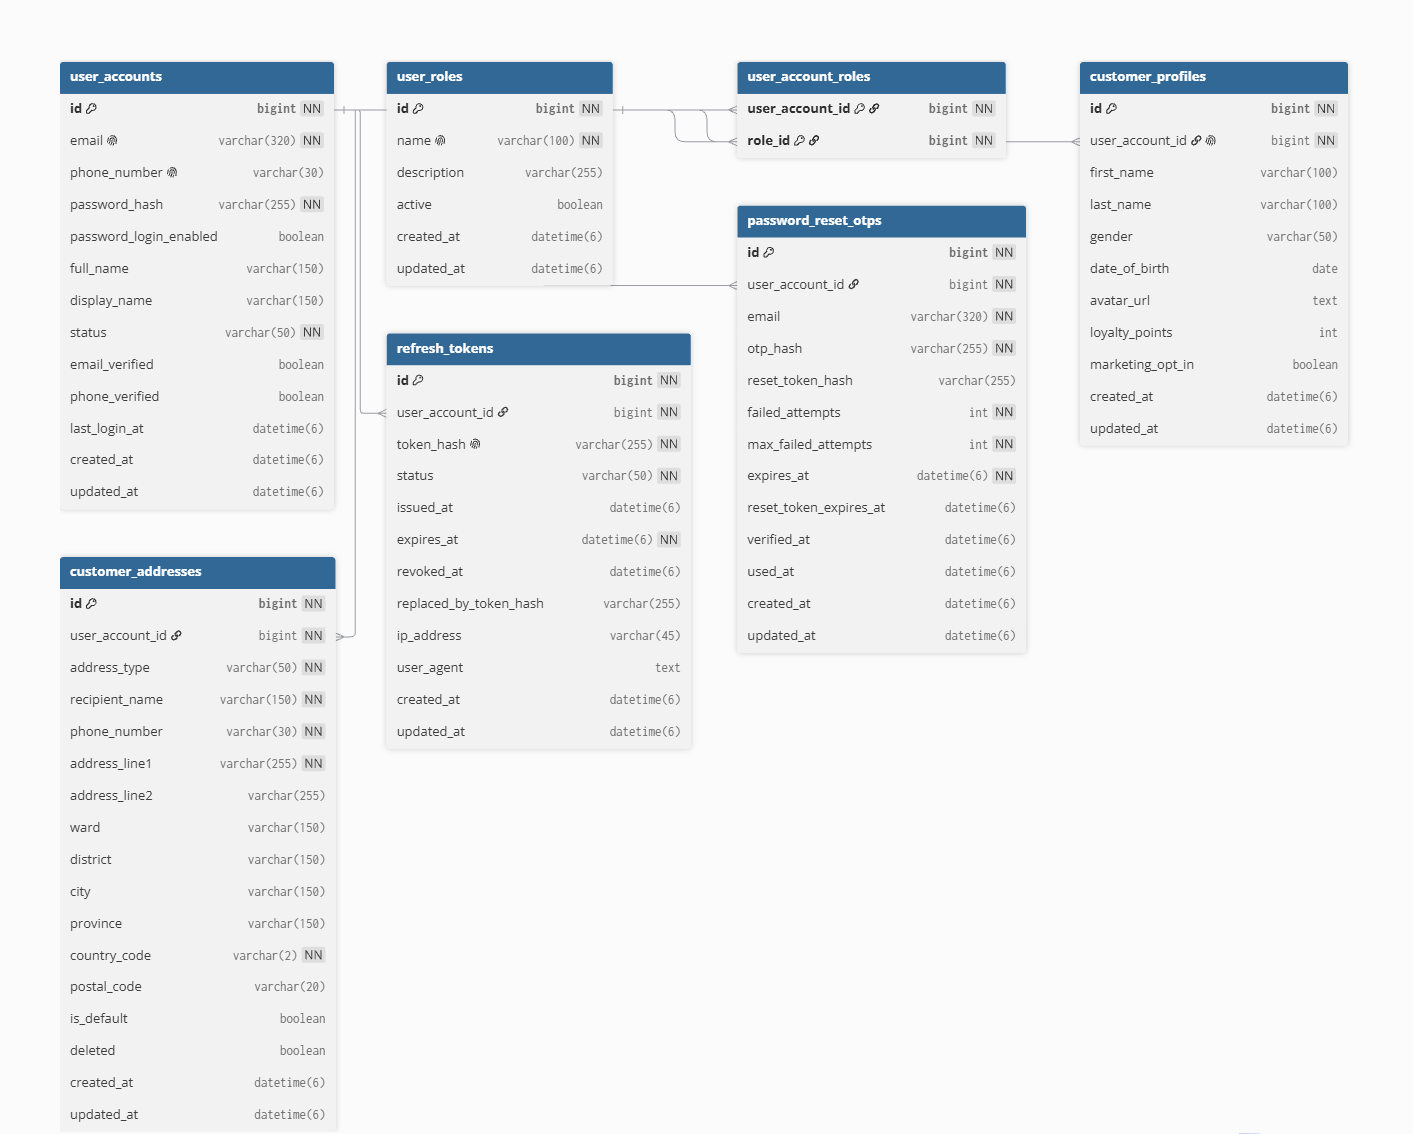
\includegraphics[
        width=\textwidth,
        height=0.72\textheight,
        keepaspectratio
    ]{Images/Thietkehethong/Người dùng và phân quyền.png}
    \caption{Sơ đồ dữ liệu người dùng và phân quyền}
    \label{fig:database-user-authorization}
\end{figure}

Trong Hình~\ref{fig:database-user-authorization}, \texttt{user\_accounts} là
thực thể trung tâm. Mỗi tài khoản có tối đa một hồ sơ khách hàng và có thể sở hữu
nhiều địa chỉ, refresh token hoặc yêu cầu đặt lại mật khẩu. Quan hệ giữa tài
khoản và vai trò được chuẩn hóa qua \texttt{user\_account\_roles}, cho phép mở
rộng tập vai trò mà không phải thay đổi cấu trúc tài khoản.

Bảng~\ref{tab:data-summary-user-authorization} tóm tắt chức năng của các bảng trong nhóm. Chỉ các bảng cốt lõi, đại diện trực tiếp cho luồng nghiệp vụ chính, được mô tả chi tiết trường dữ liệu.

\begin{longtable}{|>{\RaggedRight\arraybackslash}p{0.34\textwidth}|>{\RaggedRight\arraybackslash}p{0.56\textwidth}|}
    \caption{Các bảng thuộc nhóm người dùng và phân quyền}
    \label{tab:data-summary-user-authorization} \\
    \hline
    \textbf{Tên bảng} & \textbf{Chức năng} \\
    \hline
    \endfirsthead
    \multicolumn{2}{c}{\tablename\ \thetable\ (tiếp theo)} \\
    \hline
    \textbf{Tên bảng} & \textbf{Chức năng} \\
    \hline
    \endhead
    \texttt{user\_accounts} & Tài khoản người dùng. \\
    \hline
    \texttt{user\_roles} & Vai trò người dùng. \\
    \hline
    \texttt{user\_account\_roles} & Gán vai trò cho tài khoản. \\
    \hline
    \texttt{customer\_profiles} & Hồ sơ khách hàng. \\
    \hline
    \texttt{customer\_addresses} & Địa chỉ khách hàng. \\
    \hline
    \texttt{refresh\_tokens} & Refresh token. \\
    \hline
    \texttt{password\_reset\_otps} & Mã OTP đặt lại mật khẩu. \\
    \hline
\end{longtable}

\paragraph{Các bảng cốt lõi.}

\begin{longtable}{|>{\RaggedRight\arraybackslash}p{0.25\textwidth}|>{\RaggedRight\arraybackslash}p{0.20\textwidth}|>{\RaggedRight\arraybackslash}p{0.45\textwidth}|}
    \caption{Mô tả chi tiết bảng \texttt{user\_accounts} (Tài khoản người dùng)}
    \label{tab:data-dictionary-user-accounts} \\
    \hline
    \textbf{Tên trường} & \textbf{Kiểu dữ liệu} & \textbf{Mô tả} \\
    \hline
    \endfirsthead
    \multicolumn{3}{c}{\tablename\ \thetable\ (tiếp theo)} \\
    \hline
    \textbf{Tên trường} & \textbf{Kiểu dữ liệu} & \textbf{Mô tả} \\
    \hline
    \endhead
    \texttt{\seqsplit{id}} & \texttt{bigint} & Khóa chính tự tăng. \\
        \hline
        \texttt{\seqsplit{email}} & \texttt{varchar(320)} & Địa chỉ thư điện tử; bắt buộc; duy nhất. \\
        \hline
        \texttt{\seqsplit{phone\_number}} & \texttt{varchar(30)} & Số điện thoại; duy nhất. \\
        \hline
        \texttt{\seqsplit{password\_hash}} & \texttt{varchar(255)} & Giá trị băm của mật khẩu; bắt buộc. \\
        \hline
        \texttt{\seqsplit{password\_login\_enabled}} & \texttt{boolean} & Cho biết tài khoản có cho phép đăng nhập bằng mật khẩu. \\
        \hline
        \texttt{\seqsplit{full\_name}} & \texttt{varchar(150)} & Họ và tên đầy đủ. \\
        \hline
        \texttt{\seqsplit{display\_name}} & \texttt{varchar(150)} & Tên hiển thị. \\
        \hline
        \texttt{\seqsplit{status}} & \texttt{varchar(50)} & Trạng thái hiện tại; bắt buộc. \\
        \hline
        \texttt{\seqsplit{email\_verified}} & \texttt{boolean} & Cho biết email đã được xác minh. \\
        \hline
        \texttt{\seqsplit{phone\_verified}} & \texttt{boolean} & Cho biết số điện thoại đã được xác minh. \\
        \hline
        \texttt{\seqsplit{last\_login\_at}} & \texttt{datetime(6)} & Thời điểm đăng nhập gần nhất. \\
        \hline
        \texttt{\seqsplit{created\_at}} & \texttt{datetime(6)} & Thời điểm tạo bản ghi. \\
        \hline
        \texttt{\seqsplit{updated\_at}} & \texttt{datetime(6)} & Thời điểm cập nhật gần nhất. \\
        \hline
\end{longtable}

\begin{longtable}{|>{\RaggedRight\arraybackslash}p{0.25\textwidth}|>{\RaggedRight\arraybackslash}p{0.20\textwidth}|>{\RaggedRight\arraybackslash}p{0.45\textwidth}|}
    \caption{Mô tả chi tiết bảng \texttt{user\_roles} (Vai trò người dùng)}
    \label{tab:data-dictionary-user-roles} \\
    \hline
    \textbf{Tên trường} & \textbf{Kiểu dữ liệu} & \textbf{Mô tả} \\
    \hline
    \endfirsthead
    \multicolumn{3}{c}{\tablename\ \thetable\ (tiếp theo)} \\
    \hline
    \textbf{Tên trường} & \textbf{Kiểu dữ liệu} & \textbf{Mô tả} \\
    \hline
    \endhead
    \texttt{\seqsplit{id}} & \texttt{bigint} & Khóa chính tự tăng. \\
        \hline
        \texttt{\seqsplit{name}} & \texttt{varchar(100)} & Tên; bắt buộc; duy nhất. \\
        \hline
        \texttt{\seqsplit{description}} & \texttt{varchar(255)} & Nội dung mô tả. \\
        \hline
        \texttt{\seqsplit{active}} & \texttt{boolean} & Cho biết bản ghi đang hoạt động. \\
        \hline
        \texttt{\seqsplit{created\_at}} & \texttt{datetime(6)} & Thời điểm tạo bản ghi. \\
        \hline
        \texttt{\seqsplit{updated\_at}} & \texttt{datetime(6)} & Thời điểm cập nhật gần nhất. \\
        \hline
\end{longtable}



\subsubsection{Nhóm dữ liệu danh mục và sản phẩm}

Nhóm danh mục và sản phẩm lưu dữ liệu mô tả hàng hóa, cấu trúc danh mục, biến
thể, thuộc tính, hình ảnh và giá bán. Bảng \texttt{products} đóng vai trò trung
tâm; các quan hệ thành phần được tách thành bảng riêng để một sản phẩm có thể có
nhiều danh mục, biến thể, thuộc tính và hình ảnh mà không lặp dữ liệu nền.

\begin{figure}[H]
    \centering
    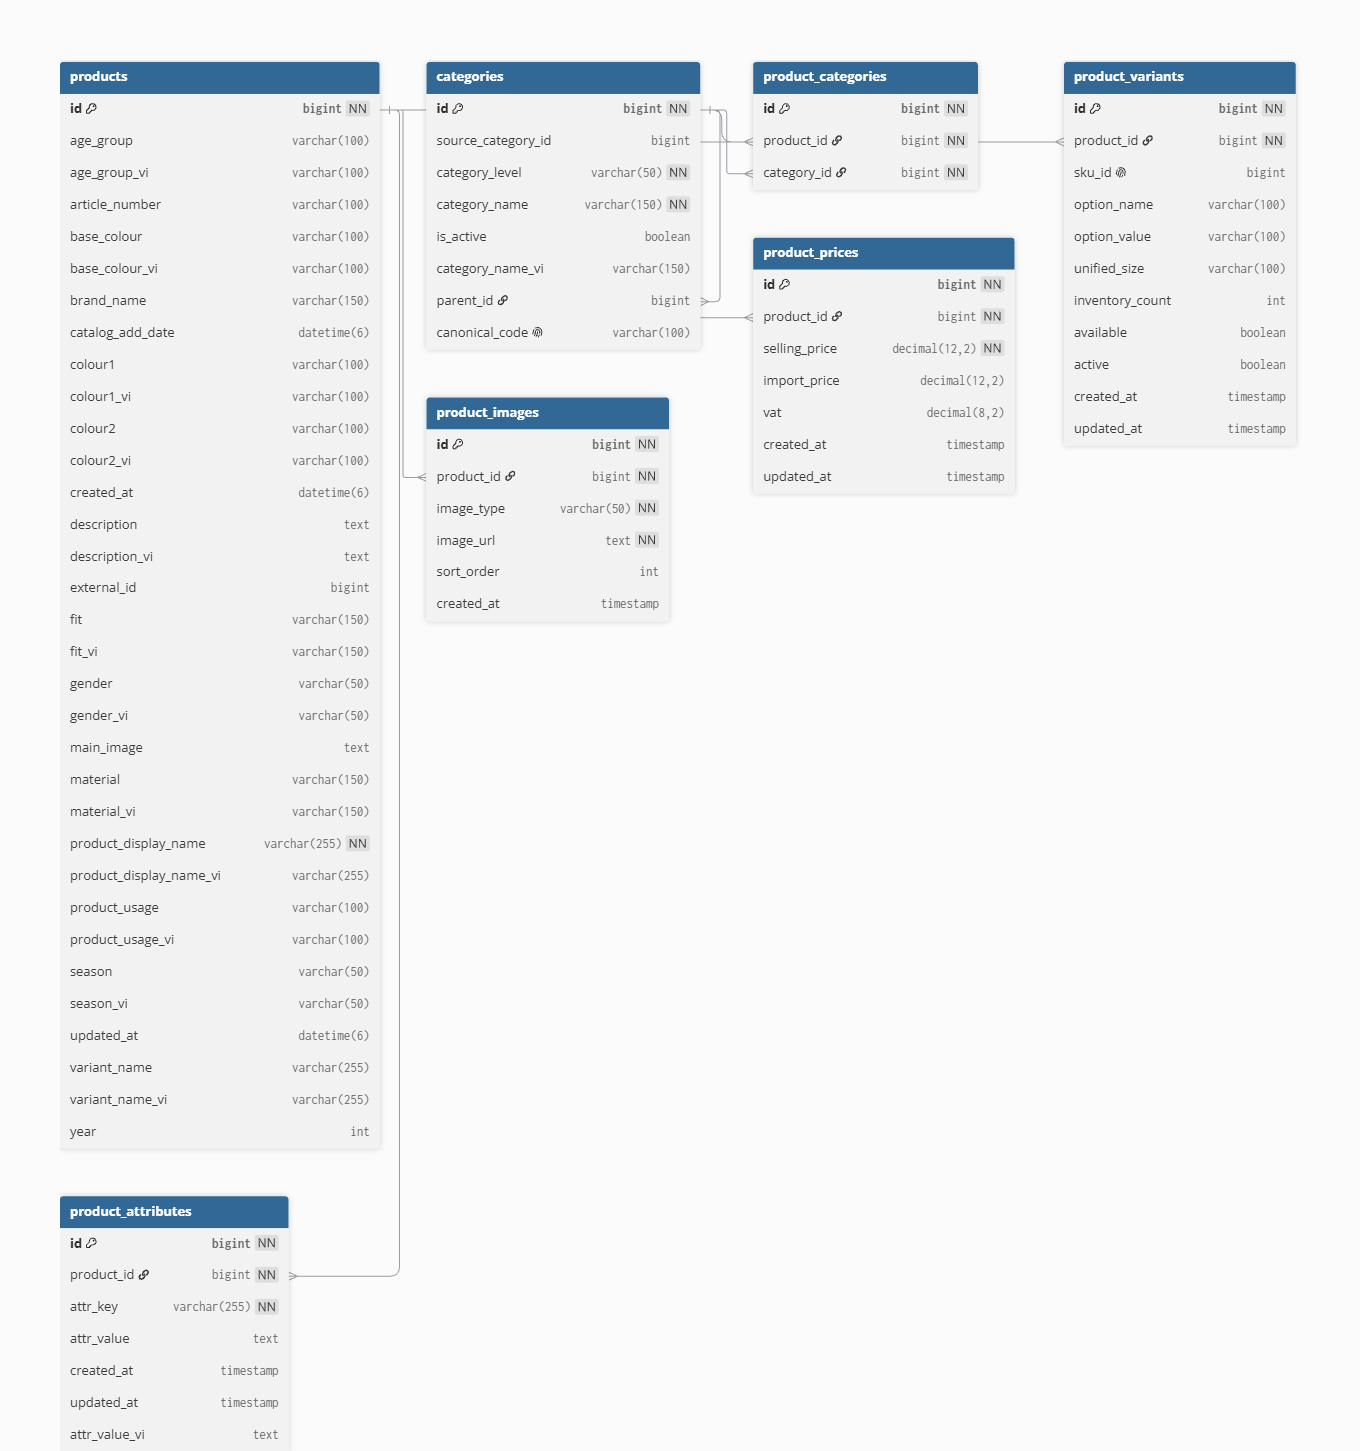
\includegraphics[
        width=\textwidth,
        height=0.72\textheight,
        keepaspectratio
    ]{Images/Thietkehethong/Danh mục và sản phẩm.png}
    \caption{Sơ đồ dữ liệu danh mục và sản phẩm}
    \label{fig:database-catalog-product}
\end{figure}

Hình~\ref{fig:database-catalog-product} cho thấy một sản phẩm có thể thuộc nhiều
danh mục thông qua bảng liên kết sản phẩm--danh mục; bản thân danh mục có quan hệ
cha--con để biểu diễn cấu trúc phân cấp. Biến thể, thuộc tính, hình ảnh và giá
được tách khỏi \texttt{products}, nhờ đó các tập dữ liệu có số lượng thay đổi
độc lập và không làm lặp lại thông tin mô tả chung của sản phẩm.

Bảng~\ref{tab:data-summary-catalog-product} tóm tắt chức năng của các bảng trong nhóm. Chỉ các bảng cốt lõi, đại diện trực tiếp cho luồng nghiệp vụ chính, được mô tả chi tiết trường dữ liệu.

\begin{longtable}{|>{\RaggedRight\arraybackslash}p{0.34\textwidth}|>{\RaggedRight\arraybackslash}p{0.56\textwidth}|}
    \caption{Các bảng thuộc nhóm danh mục và sản phẩm}
    \label{tab:data-summary-catalog-product} \\
    \hline
    \textbf{Tên bảng} & \textbf{Chức năng} \\
    \hline
    \endfirsthead
    \multicolumn{2}{c}{\tablename\ \thetable\ (tiếp theo)} \\
    \hline
    \textbf{Tên bảng} & \textbf{Chức năng} \\
    \hline
    \endhead
    \texttt{products} & Sản phẩm. \\
    \hline
    \texttt{categories} & Danh mục sản phẩm. \\
    \hline
    \texttt{product\_categories} & Liên kết sản phẩm--danh mục. \\
    \hline
    \texttt{product\_variants} & Biến thể sản phẩm. \\
    \hline
    \texttt{product\_attributes} & Thuộc tính sản phẩm. \\
    \hline
    \texttt{product\_images} & Hình ảnh sản phẩm. \\
    \hline
    \texttt{product\_prices} & Giá sản phẩm. \\
    \hline
\end{longtable}

\paragraph{Các bảng cốt lõi.}

\begin{longtable}{|>{\RaggedRight\arraybackslash}p{0.25\textwidth}|>{\RaggedRight\arraybackslash}p{0.20\textwidth}|>{\RaggedRight\arraybackslash}p{0.45\textwidth}|}
    \caption{Mô tả chi tiết bảng \texttt{products} (Sản phẩm)}
    \label{tab:data-dictionary-products} \\
    \hline
    \textbf{Tên trường} & \textbf{Kiểu dữ liệu} & \textbf{Mô tả} \\
    \hline
    \endfirsthead
    \multicolumn{3}{c}{\tablename\ \thetable\ (tiếp theo)} \\
    \hline
    \textbf{Tên trường} & \textbf{Kiểu dữ liệu} & \textbf{Mô tả} \\
    \hline
    \endhead
    \texttt{\seqsplit{id}} & \texttt{bigint} & Khóa chính. \\
        \hline
        \texttt{\seqsplit{age\_group}} & \texttt{varchar(100)} & Nhóm tuổi của sản phẩm. \\
        \hline
        \texttt{\seqsplit{age\_group\_vi}} & \texttt{varchar(100)} & Nhóm tuổi bằng tiếng Việt. \\
        \hline
        \texttt{\seqsplit{article\_number}} & \texttt{varchar(100)} & Mã bài hàng của sản phẩm. \\
        \hline
        \texttt{\seqsplit{base\_colour}} & \texttt{varchar(100)} & Màu cơ bản. \\
        \hline
        \texttt{\seqsplit{base\_colour\_vi}} & \texttt{varchar(100)} & Màu cơ bản bằng tiếng Việt. \\
        \hline
        \texttt{\seqsplit{brand\_name}} & \texttt{varchar(150)} & Tên thương hiệu. \\
        \hline
        \texttt{\seqsplit{catalog\_add\_date}} & \texttt{datetime(6)} & Thời điểm sản phẩm được thêm vào danh mục. \\
        \hline
        \texttt{\seqsplit{colour1}} & \texttt{varchar(100)} & Màu thứ nhất. \\
        \hline
        \texttt{\seqsplit{colour1\_vi}} & \texttt{varchar(100)} & Màu thứ nhất bằng tiếng Việt. \\
        \hline
        \texttt{\seqsplit{colour2}} & \texttt{varchar(100)} & Màu thứ hai. \\
        \hline
        \texttt{\seqsplit{colour2\_vi}} & \texttt{varchar(100)} & Màu thứ hai bằng tiếng Việt. \\
        \hline
        \texttt{\seqsplit{created\_at}} & \texttt{datetime(6)} & Thời điểm tạo bản ghi. \\
        \hline
        \texttt{\seqsplit{description}} & \texttt{text} & Nội dung mô tả. \\
        \hline
        \texttt{\seqsplit{description\_vi}} & \texttt{text} & Mô tả bằng tiếng Việt. \\
        \hline
        \texttt{\seqsplit{external\_id}} & \texttt{bigint} & Định danh sản phẩm tại nguồn ngoài. \\
        \hline
        \texttt{\seqsplit{fit}} & \texttt{varchar(150)} & Kiểu dáng. \\
        \hline
        \texttt{\seqsplit{fit\_vi}} & \texttt{varchar(150)} & Kiểu dáng bằng tiếng Việt. \\
        \hline
        \texttt{\seqsplit{gender}} & \texttt{varchar(50)} & Giới tính. \\
        \hline
        \texttt{\seqsplit{gender\_vi}} & \texttt{varchar(50)} & Giới tính bằng tiếng Việt. \\
        \hline
        \texttt{\seqsplit{main\_image}} & \texttt{text} & Đường dẫn ảnh đại diện chính. \\
        \hline
        \texttt{\seqsplit{material}} & \texttt{varchar(150)} & Chất liệu. \\
        \hline
        \texttt{\seqsplit{material\_vi}} & \texttt{varchar(150)} & Chất liệu bằng tiếng Việt. \\
        \hline
        \texttt{\seqsplit{product\_display\_name}} & \texttt{varchar(255)} & Tên hiển thị của sản phẩm; bắt buộc. \\
        \hline
        \texttt{\seqsplit{product\_display\_name\_vi}} & \texttt{varchar(255)} & Tên hiển thị bằng tiếng Việt. \\
        \hline
        \texttt{\seqsplit{product\_usage}} & \texttt{varchar(100)} & Mục đích sử dụng. \\
        \hline
        \texttt{\seqsplit{product\_usage\_vi}} & \texttt{varchar(100)} & Mục đích sử dụng bằng tiếng Việt. \\
        \hline
        \texttt{\seqsplit{season}} & \texttt{varchar(50)} & Mùa sử dụng. \\
        \hline
        \texttt{\seqsplit{season\_vi}} & \texttt{varchar(50)} & Mùa sử dụng bằng tiếng Việt. \\
        \hline
        \texttt{\seqsplit{updated\_at}} & \texttt{datetime(6)} & Thời điểm cập nhật gần nhất. \\
        \hline
        \texttt{\seqsplit{variant\_name}} & \texttt{varchar(255)} & Tên biến thể. \\
        \hline
        \texttt{\seqsplit{variant\_name\_vi}} & \texttt{varchar(255)} & Tên biến thể bằng tiếng Việt. \\
        \hline
        \texttt{\seqsplit{year}} & \texttt{int} & Năm của mẫu sản phẩm. \\
        \hline
\end{longtable}

\begin{longtable}{|>{\RaggedRight\arraybackslash}p{0.25\textwidth}|>{\RaggedRight\arraybackslash}p{0.20\textwidth}|>{\RaggedRight\arraybackslash}p{0.45\textwidth}|}
    \caption{Mô tả chi tiết bảng \texttt{categories} (Danh mục sản phẩm)}
    \label{tab:data-dictionary-categories} \\
    \hline
    \textbf{Tên trường} & \textbf{Kiểu dữ liệu} & \textbf{Mô tả} \\
    \hline
    \endfirsthead
    \multicolumn{3}{c}{\tablename\ \thetable\ (tiếp theo)} \\
    \hline
    \textbf{Tên trường} & \textbf{Kiểu dữ liệu} & \textbf{Mô tả} \\
    \hline
    \endhead
    \texttt{\seqsplit{id}} & \texttt{bigint} & Khóa chính tự tăng. \\
        \hline
        \texttt{\seqsplit{source\_category\_id}} & \texttt{bigint} & Định danh danh mục tại nguồn dữ liệu ngoài. \\
        \hline
        \texttt{\seqsplit{category\_level}} & \texttt{varchar(50)} & Cấp của danh mục; bắt buộc. \\
        \hline
        \texttt{\seqsplit{category\_name}} & \texttt{varchar(150)} & Tên danh mục; bắt buộc. \\
        \hline
        \texttt{\seqsplit{is\_active}} & \texttt{boolean} & Cho biết danh mục đang được kích hoạt và có thể sử dụng. \\
        \hline
        \texttt{\seqsplit{category\_name\_vi}} & \texttt{varchar(150)} & Tên danh mục bằng tiếng Việt. \\
        \hline
        \texttt{\seqsplit{parent\_id}} & \texttt{bigint} & Khóa ngoại tham chiếu \texttt{categories.id}. \\
        \hline
        \texttt{\seqsplit{canonical\_code}} & \texttt{varchar(100)} & Mã chuẩn duy nhất của danh mục; duy nhất. \\
        \hline
\end{longtable}

\begin{longtable}{|>{\RaggedRight\arraybackslash}p{0.25\textwidth}|>{\RaggedRight\arraybackslash}p{0.20\textwidth}|>{\RaggedRight\arraybackslash}p{0.45\textwidth}|}
    \caption{Mô tả chi tiết bảng \texttt{product\_images} (Hình ảnh sản phẩm)}
    \label{tab:data-dictionary-product-images} \\
    \hline
    \textbf{Tên trường} & \textbf{Kiểu dữ liệu} & \textbf{Mô tả} \\
    \hline
    \endfirsthead
    \multicolumn{3}{c}{\tablename\ \thetable\ (tiếp theo)} \\
    \hline
    \textbf{Tên trường} & \textbf{Kiểu dữ liệu} & \textbf{Mô tả} \\
    \hline
    \endhead
    \texttt{\seqsplit{id}} & \texttt{bigint} & Khóa chính tự tăng. \\
        \hline
        \texttt{\seqsplit{product\_id}} & \texttt{bigint} & Khóa ngoại tham chiếu \texttt{products.id}; bắt buộc. \\
        \hline
        \texttt{\seqsplit{image\_type}} & \texttt{varchar(50)} & Loại hình ảnh; bắt buộc. \\
        \hline
        \texttt{\seqsplit{image\_url}} & \texttt{text} & Đường dẫn hình ảnh; bắt buộc. \\
        \hline
        \texttt{\seqsplit{sort\_order}} & \texttt{int} & Thứ tự hiển thị. \\
        \hline
        \texttt{\seqsplit{created\_at}} & \texttt{timestamp} & Thời điểm tạo bản ghi. \\
        \hline
\end{longtable}



\subsubsection{Nhóm dữ liệu quản lý kho}

Nhóm quản lý kho theo dõi phần hàng được giữ tạm trong quá trình đặt mua và lịch
sử thay đổi tồn kho. Mỗi bản ghi giữ hàng gắn với sản phẩm, biến thể, người dùng
và giỏ hoặc đơn hàng tương ứng; các biến động tồn kho lưu lượng thay đổi cùng
tham chiếu nghiệp vụ để hỗ trợ đối soát và chống xử lý trùng lặp.

\begin{figure}[H]
    \centering
    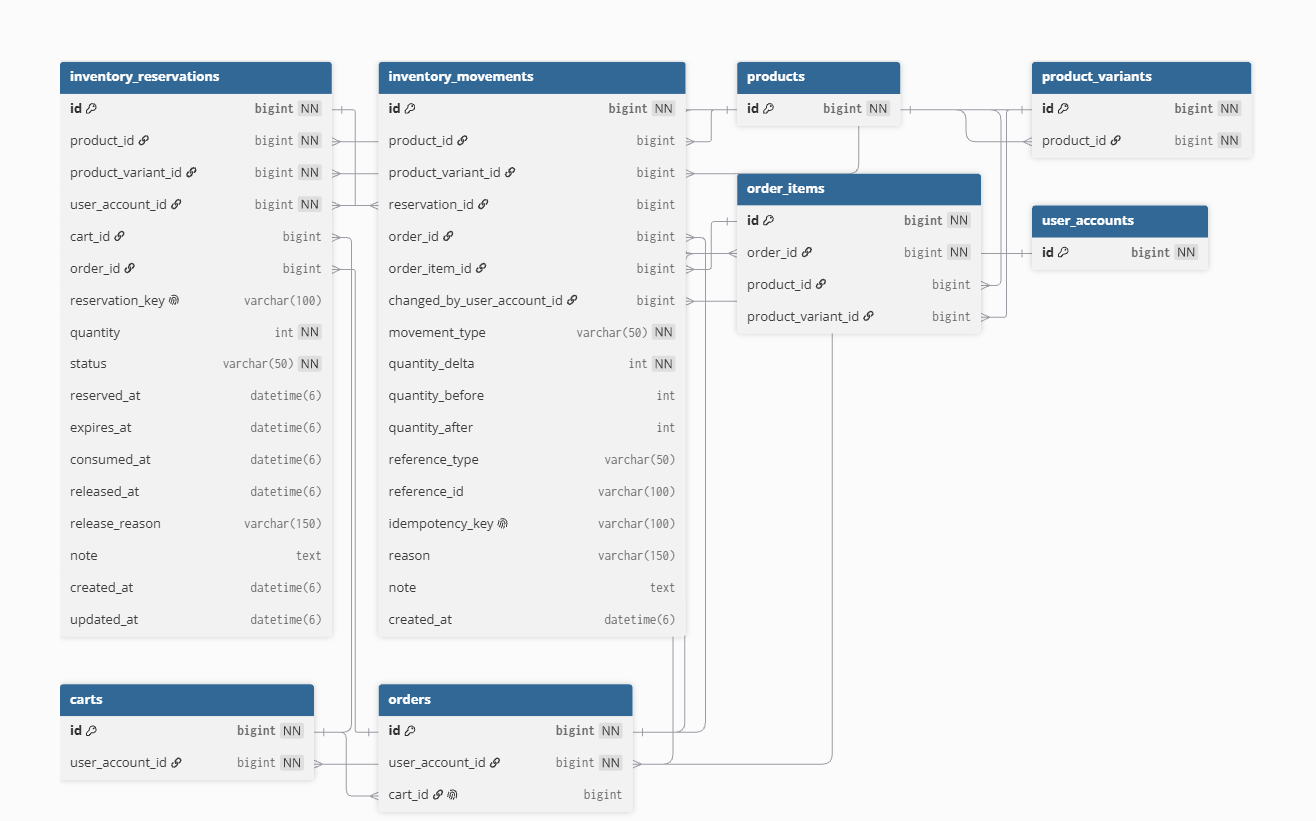
\includegraphics[
        width=\textwidth,
        height=0.72\textheight,
        keepaspectratio
    ]{Images/Thietkehethong/Quản lý kho.png}
    \caption{Sơ đồ dữ liệu quản lý kho}
    \label{fig:database-inventory}
\end{figure}

Theo Hình~\ref{fig:database-inventory},
\texttt{inventory\_reservations} biểu diễn phần tồn kho được giữ cho một người
dùng trong ngữ cảnh giỏ hàng hoặc đơn hàng. Mọi thay đổi tương ứng được ghi vào
\texttt{inventory\_movements} cùng lượng trước--sau, loại biến động và khóa
idempotency. Các bảng sản phẩm, giỏ hàng, đơn hàng và người dùng xuất hiện ở dạng
tham chiếu nhằm thể hiện nguồn phát sinh nghiệp vụ mà không lặp lại toàn bộ miền
dữ liệu liên quan.

Bảng~\ref{tab:data-summary-inventory} tóm tắt chức năng của các bảng trong nhóm. Chỉ các bảng cốt lõi, đại diện trực tiếp cho luồng nghiệp vụ chính, được mô tả chi tiết trường dữ liệu.

\begin{longtable}{|>{\RaggedRight\arraybackslash}p{0.34\textwidth}|>{\RaggedRight\arraybackslash}p{0.56\textwidth}|}
    \caption{Các bảng thuộc nhóm quản lý kho}
    \label{tab:data-summary-inventory} \\
    \hline
    \textbf{Tên bảng} & \textbf{Chức năng} \\
    \hline
    \endfirsthead
    \multicolumn{2}{c}{\tablename\ \thetable\ (tiếp theo)} \\
    \hline
    \textbf{Tên bảng} & \textbf{Chức năng} \\
    \hline
    \endhead
    \texttt{inventory\_reservations} & Giữ tồn kho. \\
    \hline
    \texttt{inventory\_movements} & Biến động tồn kho. \\
    \hline
\end{longtable}

\paragraph{Các bảng cốt lõi.}

\begin{longtable}{|>{\RaggedRight\arraybackslash}p{0.25\textwidth}|>{\RaggedRight\arraybackslash}p{0.20\textwidth}|>{\RaggedRight\arraybackslash}p{0.45\textwidth}|}
    \caption{Mô tả chi tiết bảng \texttt{inventory\_reservations} (Giữ tồn kho)}
    \label{tab:data-dictionary-inventory-reservations} \\
    \hline
    \textbf{Tên trường} & \textbf{Kiểu dữ liệu} & \textbf{Mô tả} \\
    \hline
    \endfirsthead
    \multicolumn{3}{c}{\tablename\ \thetable\ (tiếp theo)} \\
    \hline
    \textbf{Tên trường} & \textbf{Kiểu dữ liệu} & \textbf{Mô tả} \\
    \hline
    \endhead
    \texttt{\seqsplit{id}} & \texttt{bigint} & Khóa chính tự tăng. \\
        \hline
        \texttt{\seqsplit{product\_id}} & \texttt{bigint} & Khóa ngoại tham chiếu \texttt{products.id}; bắt buộc. \\
        \hline
        \texttt{\seqsplit{product\_variant\_id}} & \texttt{bigint} & Khóa ngoại tham chiếu \texttt{product\_variants.id}; bắt buộc. \\
        \hline
        \texttt{\seqsplit{user\_account\_id}} & \texttt{bigint} & Khóa ngoại tham chiếu \texttt{user\_accounts.id}; bắt buộc. \\
        \hline
        \texttt{\seqsplit{cart\_id}} & \texttt{bigint} & Khóa ngoại tham chiếu \texttt{carts.id}. \\
        \hline
        \texttt{\seqsplit{order\_id}} & \texttt{bigint} & Khóa ngoại tham chiếu \texttt{orders.id}. \\
        \hline
        \texttt{\seqsplit{reservation\_key}} & \texttt{varchar(100)} & Khóa duy nhất chống giữ tồn kho trùng; duy nhất. \\
        \hline
        \texttt{\seqsplit{quantity}} & \texttt{int} & Số lượng; bắt buộc. \\
        \hline
        \texttt{\seqsplit{status}} & \texttt{varchar(50)} & Trạng thái hiện tại; bắt buộc. \\
        \hline
        \texttt{\seqsplit{reserved\_at}} & \texttt{datetime(6)} & Thời điểm giữ hàng. \\
        \hline
        \texttt{\seqsplit{expires\_at}} & \texttt{datetime(6)} & Thời điểm hết hiệu lực. \\
        \hline
        \texttt{\seqsplit{consumed\_at}} & \texttt{datetime(6)} & Thời điểm phần giữ hàng được sử dụng. \\
        \hline
        \texttt{\seqsplit{released\_at}} & \texttt{datetime(6)} & Thời điểm giải phóng phần giữ hàng. \\
        \hline
        \texttt{\seqsplit{release\_reason}} & \texttt{varchar(150)} & Lý do giải phóng. \\
        \hline
        \texttt{\seqsplit{note}} & \texttt{text} & Ghi chú. \\
        \hline
        \texttt{\seqsplit{created\_at}} & \texttt{datetime(6)} & Thời điểm tạo bản ghi. \\
        \hline
        \texttt{\seqsplit{updated\_at}} & \texttt{datetime(6)} & Thời điểm cập nhật gần nhất. \\
        \hline
\end{longtable}

\begin{longtable}{|>{\RaggedRight\arraybackslash}p{0.25\textwidth}|>{\RaggedRight\arraybackslash}p{0.20\textwidth}|>{\RaggedRight\arraybackslash}p{0.45\textwidth}|}
    \caption{Mô tả chi tiết bảng \texttt{inventory\_movements} (Biến động tồn kho)}
    \label{tab:data-dictionary-inventory-movements} \\
    \hline
    \textbf{Tên trường} & \textbf{Kiểu dữ liệu} & \textbf{Mô tả} \\
    \hline
    \endfirsthead
    \multicolumn{3}{c}{\tablename\ \thetable\ (tiếp theo)} \\
    \hline
    \textbf{Tên trường} & \textbf{Kiểu dữ liệu} & \textbf{Mô tả} \\
    \hline
    \endhead
    \texttt{\seqsplit{id}} & \texttt{bigint} & Khóa chính tự tăng. \\
        \hline
        \texttt{\seqsplit{product\_id}} & \texttt{bigint} & Khóa ngoại tham chiếu \texttt{products.id}. \\
        \hline
        \texttt{\seqsplit{product\_variant\_id}} & \texttt{bigint} & Khóa ngoại tham chiếu \texttt{product\_variants.id}. \\
        \hline
        \texttt{\seqsplit{reservation\_id}} & \texttt{bigint} & Khóa ngoại tham chiếu \texttt{inventory\_reservations.id}. \\
        \hline
        \texttt{\seqsplit{order\_id}} & \texttt{bigint} & Khóa ngoại tham chiếu \texttt{orders.id}. \\
        \hline
        \texttt{\seqsplit{order\_item\_id}} & \texttt{bigint} & Khóa ngoại tham chiếu \texttt{order\_items.id}. \\
        \hline
        \texttt{\seqsplit{changed\_by\_user\_account\_id}} & \texttt{bigint} & Khóa ngoại tham chiếu \texttt{user\_accounts.id}. \\
        \hline
        \texttt{\seqsplit{movement\_type}} & \texttt{varchar(50)} & Loại biến động tồn kho; bắt buộc. \\
        \hline
        \texttt{\seqsplit{quantity\_delta}} & \texttt{int} & Lượng tồn kho thay đổi; bắt buộc. \\
        \hline
        \texttt{\seqsplit{quantity\_before}} & \texttt{int} & Số lượng trước biến động. \\
        \hline
        \texttt{\seqsplit{quantity\_after}} & \texttt{int} & Số lượng sau biến động. \\
        \hline
        \texttt{\seqsplit{reference\_type}} & \texttt{varchar(50)} & Loại đối tượng nghiệp vụ tham chiếu. \\
        \hline
        \texttt{\seqsplit{reference\_id}} & \texttt{varchar(100)} & Định danh đối tượng nghiệp vụ tham chiếu. \\
        \hline
        \texttt{\seqsplit{idempotency\_key}} & \texttt{varchar(100)} & Khóa duy nhất chống xử lý lặp; duy nhất. \\
        \hline
        \texttt{\seqsplit{reason}} & \texttt{varchar(150)} & Lý do. \\
        \hline
        \texttt{\seqsplit{note}} & \texttt{text} & Ghi chú. \\
        \hline
        \texttt{\seqsplit{created\_at}} & \texttt{datetime(6)} & Thời điểm tạo bản ghi. \\
        \hline
\end{longtable}



\subsubsection{Nhóm dữ liệu giỏ hàng và tương tác khách hàng}

Nhóm này lưu trạng thái giỏ hàng, các mặt hàng khách đã chọn, danh sách yêu thích,
đánh giá sản phẩm và nội dung blog phục vụ tương tác. Thông tin tổng hợp đánh giá
được tách khỏi đánh giá chi tiết để việc hiển thị số lượng và điểm trung bình
không phải tính lại trên toàn bộ dữ liệu sau mỗi truy vấn.

\begin{figure}[H]
    \centering
    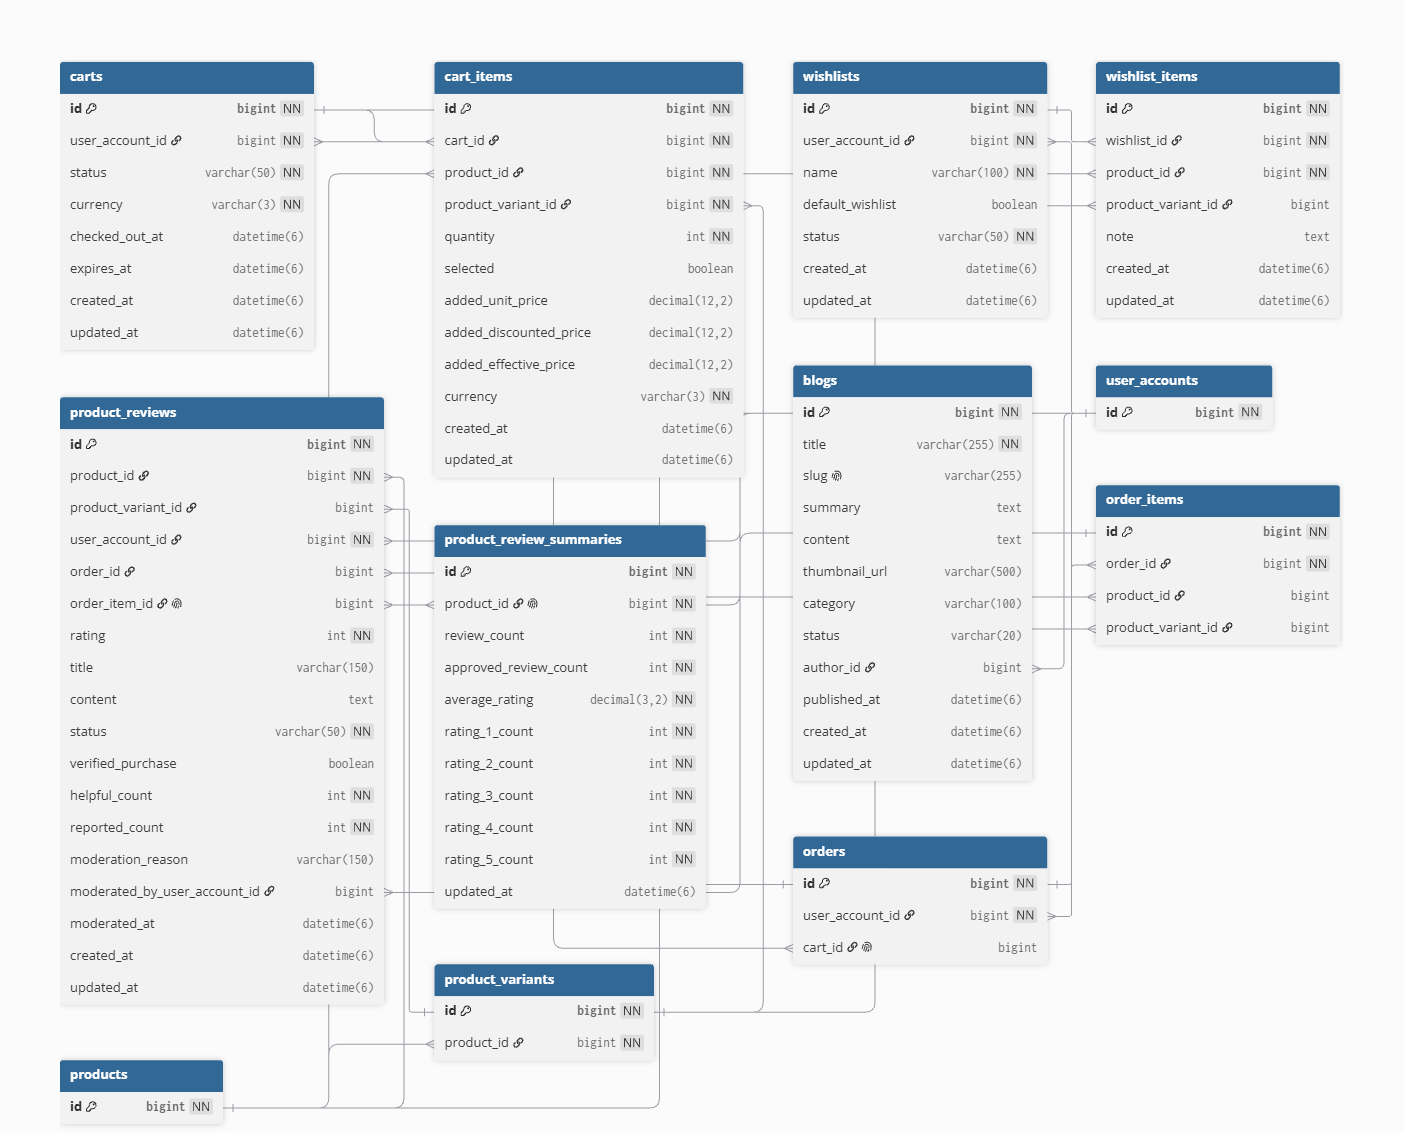
\includegraphics[
        width=\textwidth,
        height=0.72\textheight,
        keepaspectratio
    ]{Images/Thietkehethong/Giỏ hàng và tương tác khách hàng.png}
    \caption{Sơ đồ dữ liệu giỏ hàng và tương tác khách hàng}
    \label{fig:database-cart-engagement}
\end{figure}

Hình~\ref{fig:database-cart-engagement} tập hợp các dữ liệu phát sinh từ quá
trình tương tác của khách hàng. Giỏ hàng và danh sách yêu thích đều được tổ chức
theo mô hình bảng đầu mục--chi tiết. Đánh giá liên kết với người dùng, sản phẩm
và dòng đơn hàng để xác minh giao dịch mua, trong khi
\texttt{product\_review\_summaries} lưu kết quả tổng hợp phục vụ truy vấn đọc.
Bài viết blog liên kết tùy chọn với tài khoản tác giả và không phụ thuộc vào vòng
đời mua hàng.

Bảng~\ref{tab:data-summary-cart-engagement} tóm tắt chức năng của các bảng trong nhóm. Chỉ các bảng cốt lõi, đại diện trực tiếp cho luồng nghiệp vụ chính, được mô tả chi tiết trường dữ liệu.

\begin{longtable}{|>{\RaggedRight\arraybackslash}p{0.34\textwidth}|>{\RaggedRight\arraybackslash}p{0.56\textwidth}|}
    \caption{Các bảng thuộc nhóm giỏ hàng và tương tác khách hàng}
    \label{tab:data-summary-cart-engagement} \\
    \hline
    \textbf{Tên bảng} & \textbf{Chức năng} \\
    \hline
    \endfirsthead
    \multicolumn{2}{c}{\tablename\ \thetable\ (tiếp theo)} \\
    \hline
    \textbf{Tên bảng} & \textbf{Chức năng} \\
    \hline
    \endhead
    \texttt{carts} & Giỏ hàng. \\
    \hline
    \texttt{cart\_items} & Chi tiết giỏ hàng. \\
    \hline
    \texttt{wishlists} & Danh sách yêu thích. \\
    \hline
    \texttt{wishlist\_items} & Chi tiết danh sách yêu thích. \\
    \hline
    \texttt{product\_reviews} & Đánh giá sản phẩm. \\
    \hline
    \texttt{product\_review\_summaries} & Tổng hợp đánh giá sản phẩm. \\
    \hline
    \texttt{blogs} & Bài viết. \\
    \hline
\end{longtable}

\paragraph{Các bảng cốt lõi.}

\begin{longtable}{|>{\RaggedRight\arraybackslash}p{0.25\textwidth}|>{\RaggedRight\arraybackslash}p{0.20\textwidth}|>{\RaggedRight\arraybackslash}p{0.45\textwidth}|}
    \caption{Mô tả chi tiết bảng \texttt{carts} (Giỏ hàng)}
    \label{tab:data-dictionary-carts} \\
    \hline
    \textbf{Tên trường} & \textbf{Kiểu dữ liệu} & \textbf{Mô tả} \\
    \hline
    \endfirsthead
    \multicolumn{3}{c}{\tablename\ \thetable\ (tiếp theo)} \\
    \hline
    \textbf{Tên trường} & \textbf{Kiểu dữ liệu} & \textbf{Mô tả} \\
    \hline
    \endhead
    \texttt{\seqsplit{id}} & \texttt{bigint} & Khóa chính tự tăng. \\
        \hline
        \texttt{\seqsplit{user\_account\_id}} & \texttt{bigint} & Khóa ngoại tham chiếu \texttt{user\_accounts.id}; bắt buộc. \\
        \hline
        \texttt{\seqsplit{status}} & \texttt{varchar(50)} & Trạng thái hiện tại; bắt buộc. \\
        \hline
        \texttt{\seqsplit{currency}} & \texttt{varchar(3)} & Mã tiền tệ ISO 4217; bắt buộc. \\
        \hline
        \texttt{\seqsplit{checked\_out\_at}} & \texttt{datetime(6)} & Thời điểm giỏ hàng được chuyển thành đơn. \\
        \hline
        \texttt{\seqsplit{expires\_at}} & \texttt{datetime(6)} & Thời điểm hết hiệu lực. \\
        \hline
        \texttt{\seqsplit{created\_at}} & \texttt{datetime(6)} & Thời điểm tạo bản ghi. \\
        \hline
        \texttt{\seqsplit{updated\_at}} & \texttt{datetime(6)} & Thời điểm cập nhật gần nhất. \\
        \hline
\end{longtable}

\begin{longtable}{|>{\RaggedRight\arraybackslash}p{0.25\textwidth}|>{\RaggedRight\arraybackslash}p{0.20\textwidth}|>{\RaggedRight\arraybackslash}p{0.45\textwidth}|}
    \caption{Mô tả chi tiết bảng \texttt{cart\_items} (Chi tiết giỏ hàng)}
    \label{tab:data-dictionary-cart-items} \\
    \hline
    \textbf{Tên trường} & \textbf{Kiểu dữ liệu} & \textbf{Mô tả} \\
    \hline
    \endfirsthead
    \multicolumn{3}{c}{\tablename\ \thetable\ (tiếp theo)} \\
    \hline
    \textbf{Tên trường} & \textbf{Kiểu dữ liệu} & \textbf{Mô tả} \\
    \hline
    \endhead
    \texttt{\seqsplit{id}} & \texttt{bigint} & Khóa chính tự tăng. \\
        \hline
        \texttt{\seqsplit{cart\_id}} & \texttt{bigint} & Khóa ngoại tham chiếu \texttt{carts.id}; bắt buộc. \\
        \hline
        \texttt{\seqsplit{product\_id}} & \texttt{bigint} & Khóa ngoại tham chiếu \texttt{products.id}; bắt buộc. \\
        \hline
        \texttt{\seqsplit{product\_variant\_id}} & \texttt{bigint} & Khóa ngoại tham chiếu \texttt{product\_variants.id}; bắt buộc. \\
        \hline
        \texttt{\seqsplit{quantity}} & \texttt{int} & Số lượng; bắt buộc. \\
        \hline
        \texttt{\seqsplit{selected}} & \texttt{boolean} & Cho biết mặt hàng được chọn. \\
        \hline
        \texttt{\seqsplit{added\_unit\_price}} & \texttt{decimal(12,2)} & Đơn giá tại thời điểm thêm vào giỏ. \\
        \hline
        \texttt{\seqsplit{added\_discounted\_price}} & \texttt{decimal(12,2)} & Đơn giá sau giảm tại thời điểm thêm vào giỏ. \\
        \hline
        \texttt{\seqsplit{added\_effective\_price}} & \texttt{decimal(12,2)} & Đơn giá hiệu lực tại thời điểm thêm vào giỏ. \\
        \hline
        \texttt{\seqsplit{currency}} & \texttt{varchar(3)} & Mã tiền tệ ISO 4217; bắt buộc. \\
        \hline
        \texttt{\seqsplit{created\_at}} & \texttt{datetime(6)} & Thời điểm tạo bản ghi. \\
        \hline
        \texttt{\seqsplit{updated\_at}} & \texttt{datetime(6)} & Thời điểm cập nhật gần nhất. \\
        \hline
\end{longtable}

\begin{longtable}{|>{\RaggedRight\arraybackslash}p{0.25\textwidth}|>{\RaggedRight\arraybackslash}p{0.20\textwidth}|>{\RaggedRight\arraybackslash}p{0.45\textwidth}|}
    \caption{Mô tả chi tiết bảng \texttt{product\_reviews} (Đánh giá sản phẩm)}
    \label{tab:data-dictionary-product-reviews} \\
    \hline
    \textbf{Tên trường} & \textbf{Kiểu dữ liệu} & \textbf{Mô tả} \\
    \hline
    \endfirsthead
    \multicolumn{3}{c}{\tablename\ \thetable\ (tiếp theo)} \\
    \hline
    \textbf{Tên trường} & \textbf{Kiểu dữ liệu} & \textbf{Mô tả} \\
    \hline
    \endhead
    \texttt{\seqsplit{id}} & \texttt{bigint} & Khóa chính tự tăng. \\
        \hline
        \texttt{\seqsplit{product\_id}} & \texttt{bigint} & Khóa ngoại tham chiếu \texttt{products.id}; bắt buộc. \\
        \hline
        \texttt{\seqsplit{product\_variant\_id}} & \texttt{bigint} & Khóa ngoại tham chiếu \texttt{product\_variants.id}. \\
        \hline
        \texttt{\seqsplit{user\_account\_id}} & \texttt{bigint} & Khóa ngoại tham chiếu \texttt{user\_accounts.id}; bắt buộc. \\
        \hline
        \texttt{\seqsplit{order\_id}} & \texttt{bigint} & Khóa ngoại tham chiếu \texttt{orders.id}. \\
        \hline
        \texttt{\seqsplit{order\_item\_id}} & \texttt{bigint} & Khóa ngoại tham chiếu \texttt{order\_items.id}; duy nhất. \\
        \hline
        \texttt{\seqsplit{rating}} & \texttt{int} & Điểm đánh giá; bắt buộc. \\
        \hline
        \texttt{\seqsplit{title}} & \texttt{varchar(150)} & Tiêu đề. \\
        \hline
        \texttt{\seqsplit{content}} & \texttt{text} & Nội dung. \\
        \hline
        \texttt{\seqsplit{status}} & \texttt{varchar(50)} & Trạng thái hiện tại; bắt buộc. \\
        \hline
        \texttt{\seqsplit{verified\_purchase}} & \texttt{boolean} & Cho biết đánh giá phát sinh từ giao dịch đã xác minh. \\
        \hline
        \texttt{\seqsplit{helpful\_count}} & \texttt{int} & Số lượt đánh dấu hữu ích; bắt buộc. \\
        \hline
        \texttt{\seqsplit{reported\_count}} & \texttt{int} & Số lượt báo cáo; bắt buộc. \\
        \hline
        \texttt{\seqsplit{moderation\_reason}} & \texttt{varchar(150)} & Lý do kiểm duyệt. \\
        \hline
        \texttt{\seqsplit{moderated\_by\_user\_account\_id}} & \texttt{bigint} & Khóa ngoại tham chiếu \texttt{user\_accounts.id}. \\
        \hline
        \texttt{\seqsplit{moderated\_at}} & \texttt{datetime(6)} & Thời điểm kiểm duyệt. \\
        \hline
        \texttt{\seqsplit{created\_at}} & \texttt{datetime(6)} & Thời điểm tạo bản ghi. \\
        \hline
        \texttt{\seqsplit{updated\_at}} & \texttt{datetime(6)} & Thời điểm cập nhật gần nhất. \\
        \hline
\end{longtable}



\subsubsection{Nhóm dữ liệu đơn hàng và vận chuyển}

Nhóm đơn hàng lưu kết quả của quá trình mua sắm, các dòng hàng, bản chụp địa chỉ
nhận hàng và lịch sử chuyển trạng thái. Giá, tên và thuộc tính cần thiết của sản
phẩm được chụp lại trong \texttt{order\_items}; do đó nội dung đơn đã phát sinh
không bị thay đổi khi dữ liệu sản phẩm hiện hành được cập nhật hoặc xóa.

\begin{figure}[H]
    \centering
    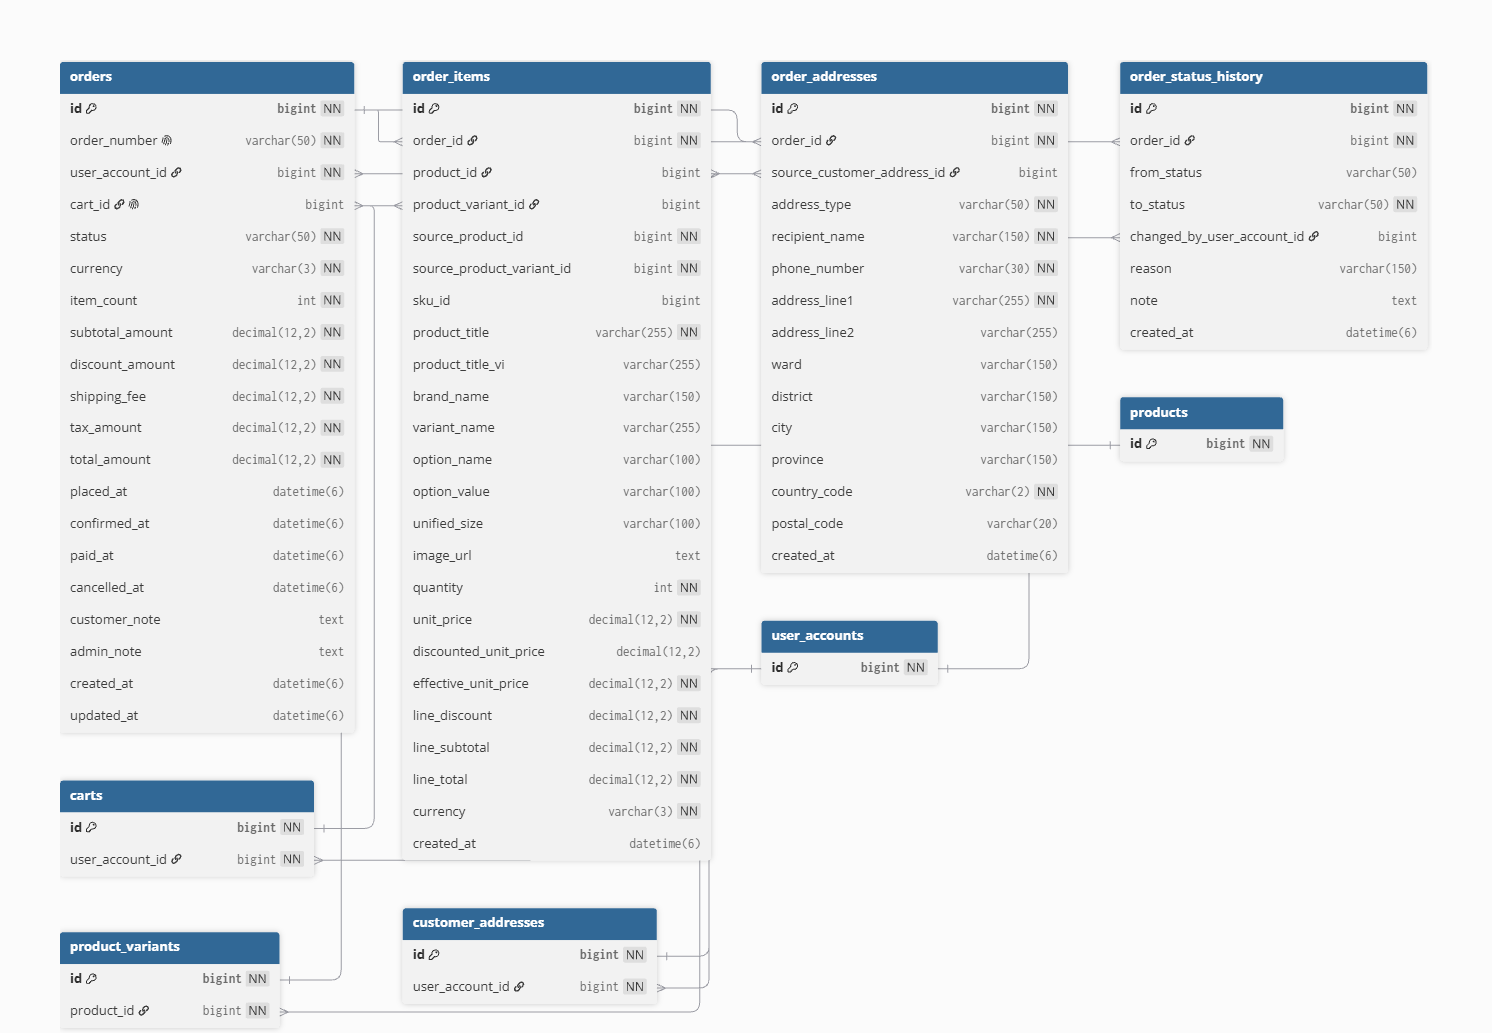
\includegraphics[
        width=\textwidth,
        height=0.72\textheight,
        keepaspectratio
    ]{Images/Thietkehethong/Đơn hàng và vận chuyển.png}
    \caption{Sơ đồ dữ liệu đơn hàng và vận chuyển}
    \label{fig:database-order-shipping}
\end{figure}

Trong Hình~\ref{fig:database-order-shipping}, \texttt{orders} liên kết một--nhiều
với các dòng hàng, địa chỉ chụp tại thời điểm đặt và lịch sử trạng thái. Liên kết
đến sản phẩm và biến thể được phép rỗng để đơn hàng cũ vẫn tồn tại khi dữ liệu
danh mục thay đổi. Tương tự, \texttt{order\_addresses} giữ bản sao địa chỉ giao
nhận thay vì phụ thuộc hoàn toàn vào địa chỉ hiện hành trong hồ sơ khách hàng.

Bảng~\ref{tab:data-summary-order-shipping} tóm tắt chức năng của các bảng trong nhóm. Chỉ các bảng cốt lõi, đại diện trực tiếp cho luồng nghiệp vụ chính, được mô tả chi tiết trường dữ liệu.

\begin{longtable}{|>{\RaggedRight\arraybackslash}p{0.34\textwidth}|>{\RaggedRight\arraybackslash}p{0.56\textwidth}|}
    \caption{Các bảng thuộc nhóm đơn hàng và vận chuyển}
    \label{tab:data-summary-order-shipping} \\
    \hline
    \textbf{Tên bảng} & \textbf{Chức năng} \\
    \hline
    \endfirsthead
    \multicolumn{2}{c}{\tablename\ \thetable\ (tiếp theo)} \\
    \hline
    \textbf{Tên bảng} & \textbf{Chức năng} \\
    \hline
    \endhead
    \texttt{orders} & Đơn hàng. \\
    \hline
    \texttt{order\_items} & Chi tiết đơn hàng. \\
    \hline
    \texttt{order\_addresses} & Địa chỉ đơn hàng. \\
    \hline
    \texttt{order\_status\_history} & Lịch sử trạng thái đơn hàng. \\
    \hline
\end{longtable}

\paragraph{Các bảng cốt lõi.}

\begin{longtable}{|>{\RaggedRight\arraybackslash}p{0.25\textwidth}|>{\RaggedRight\arraybackslash}p{0.20\textwidth}|>{\RaggedRight\arraybackslash}p{0.45\textwidth}|}
    \caption{Mô tả chi tiết bảng \texttt{orders} (Đơn hàng)}
    \label{tab:data-dictionary-orders} \\
    \hline
    \textbf{Tên trường} & \textbf{Kiểu dữ liệu} & \textbf{Mô tả} \\
    \hline
    \endfirsthead
    \multicolumn{3}{c}{\tablename\ \thetable\ (tiếp theo)} \\
    \hline
    \textbf{Tên trường} & \textbf{Kiểu dữ liệu} & \textbf{Mô tả} \\
    \hline
    \endhead
    \texttt{\seqsplit{id}} & \texttt{bigint} & Khóa chính tự tăng. \\
        \hline
        \texttt{\seqsplit{order\_number}} & \texttt{varchar(50)} & Mã đơn hàng duy nhất; bắt buộc; duy nhất. \\
        \hline
        \texttt{\seqsplit{user\_account\_id}} & \texttt{bigint} & Khóa ngoại tham chiếu \texttt{user\_accounts.id}; bắt buộc. \\
        \hline
        \texttt{\seqsplit{cart\_id}} & \texttt{bigint} & Khóa ngoại tham chiếu \texttt{carts.id}; duy nhất. \\
        \hline
        \texttt{\seqsplit{status}} & \texttt{varchar(50)} & Trạng thái hiện tại; bắt buộc. \\
        \hline
        \texttt{\seqsplit{currency}} & \texttt{varchar(3)} & Mã tiền tệ ISO 4217; bắt buộc. \\
        \hline
        \texttt{\seqsplit{item\_count}} & \texttt{int} & Tổng số mặt hàng trong đơn; bắt buộc. \\
        \hline
        \texttt{\seqsplit{subtotal\_amount}} & \texttt{decimal(12,2)} & Tạm tính trước giảm giá và phí; bắt buộc. \\
        \hline
        \texttt{\seqsplit{discount\_amount}} & \texttt{decimal(12,2)} & Tổng số tiền được giảm; bắt buộc. \\
        \hline
        \texttt{\seqsplit{shipping\_fee}} & \texttt{decimal(12,2)} & Phí vận chuyển; bắt buộc. \\
        \hline
        \texttt{\seqsplit{tax\_amount}} & \texttt{decimal(12,2)} & Tiền thuế; bắt buộc. \\
        \hline
        \texttt{\seqsplit{total\_amount}} & \texttt{decimal(12,2)} & Tổng tiền phải thanh toán; bắt buộc. \\
        \hline
        \texttt{\seqsplit{placed\_at}} & \texttt{datetime(6)} & Thời điểm đặt hàng. \\
        \hline
        \texttt{\seqsplit{confirmed\_at}} & \texttt{datetime(6)} & Thời điểm xác nhận đơn. \\
        \hline
        \texttt{\seqsplit{paid\_at}} & \texttt{datetime(6)} & Thời điểm thanh toán thành công. \\
        \hline
        \texttt{\seqsplit{cancelled\_at}} & \texttt{datetime(6)} & Thời điểm hủy. \\
        \hline
        \texttt{\seqsplit{customer\_note}} & \texttt{text} & Ghi chú của khách hàng. \\
        \hline
        \texttt{\seqsplit{admin\_note}} & \texttt{text} & Ghi chú quản trị. \\
        \hline
        \texttt{\seqsplit{created\_at}} & \texttt{datetime(6)} & Thời điểm tạo bản ghi. \\
        \hline
        \texttt{\seqsplit{updated\_at}} & \texttt{datetime(6)} & Thời điểm cập nhật gần nhất. \\
        \hline
\end{longtable}

\begin{longtable}{|>{\RaggedRight\arraybackslash}p{0.25\textwidth}|>{\RaggedRight\arraybackslash}p{0.20\textwidth}|>{\RaggedRight\arraybackslash}p{0.45\textwidth}|}
    \caption{Mô tả chi tiết bảng \texttt{order\_items} (Chi tiết đơn hàng)}
    \label{tab:data-dictionary-order-items} \\
    \hline
    \textbf{Tên trường} & \textbf{Kiểu dữ liệu} & \textbf{Mô tả} \\
    \hline
    \endfirsthead
    \multicolumn{3}{c}{\tablename\ \thetable\ (tiếp theo)} \\
    \hline
    \textbf{Tên trường} & \textbf{Kiểu dữ liệu} & \textbf{Mô tả} \\
    \hline
    \endhead
    \texttt{\seqsplit{id}} & \texttt{bigint} & Khóa chính tự tăng. \\
        \hline
        \texttt{\seqsplit{order\_id}} & \texttt{bigint} & Khóa ngoại tham chiếu \texttt{orders.id}; bắt buộc. \\
        \hline
        \texttt{\seqsplit{product\_id}} & \texttt{bigint} & Khóa ngoại tham chiếu \texttt{products.id}. \\
        \hline
        \texttt{\seqsplit{product\_variant\_id}} & \texttt{bigint} & Khóa ngoại tham chiếu \texttt{product\_variants.id}. \\
        \hline
        \texttt{\seqsplit{source\_product\_id}} & \texttt{bigint} & Định danh sản phẩm nguồn được chụp tại thời điểm mua; bắt buộc. \\
        \hline
        \texttt{\seqsplit{source\_product\_variant\_id}} & \texttt{bigint} & Định danh biến thể nguồn được chụp tại thời điểm mua; bắt buộc. \\
        \hline
        \texttt{\seqsplit{sku\_id}} & \texttt{bigint} & Định danh SKU. \\
        \hline
        \texttt{\seqsplit{product\_title}} & \texttt{varchar(255)} & Tên sản phẩm được chụp tại thời điểm mua; bắt buộc. \\
        \hline
        \texttt{\seqsplit{product\_title\_vi}} & \texttt{varchar(255)} & Tên sản phẩm tiếng Việt được chụp tại thời điểm mua. \\
        \hline
        \texttt{\seqsplit{brand\_name}} & \texttt{varchar(150)} & Tên thương hiệu. \\
        \hline
        \texttt{\seqsplit{variant\_name}} & \texttt{varchar(255)} & Tên biến thể. \\
        \hline
        \texttt{\seqsplit{option\_name}} & \texttt{varchar(100)} & Tên tùy chọn biến thể. \\
        \hline
        \texttt{\seqsplit{option\_value}} & \texttt{varchar(100)} & Giá trị tùy chọn biến thể. \\
        \hline
        \texttt{\seqsplit{unified\_size}} & \texttt{varchar(100)} & Kích cỡ đã chuẩn hóa. \\
        \hline
        \texttt{\seqsplit{image\_url}} & \texttt{text} & Đường dẫn hình ảnh. \\
        \hline
        \texttt{\seqsplit{quantity}} & \texttt{int} & Số lượng; bắt buộc. \\
        \hline
        \texttt{\seqsplit{unit\_price}} & \texttt{decimal(12,2)} & Đơn giá gốc; bắt buộc. \\
        \hline
        \texttt{\seqsplit{discounted\_unit\_price}} & \texttt{decimal(12,2)} & Đơn giá sau giảm. \\
        \hline
        \texttt{\seqsplit{effective\_unit\_price}} & \texttt{decimal(12,2)} & Đơn giá thực tế áp dụng; bắt buộc. \\
        \hline
        \texttt{\seqsplit{line\_discount}} & \texttt{decimal(12,2)} & Tiền giảm của dòng hàng; bắt buộc. \\
        \hline
        \texttt{\seqsplit{line\_subtotal}} & \texttt{decimal(12,2)} & Tạm tính của dòng hàng; bắt buộc. \\
        \hline
        \texttt{\seqsplit{line\_total}} & \texttt{decimal(12,2)} & Thành tiền của dòng hàng; bắt buộc. \\
        \hline
        \texttt{\seqsplit{currency}} & \texttt{varchar(3)} & Mã tiền tệ ISO 4217; bắt buộc. \\
        \hline
        \texttt{\seqsplit{created\_at}} & \texttt{datetime(6)} & Thời điểm tạo bản ghi. \\
        \hline
\end{longtable}

\begin{longtable}{|>{\RaggedRight\arraybackslash}p{0.25\textwidth}|>{\RaggedRight\arraybackslash}p{0.20\textwidth}|>{\RaggedRight\arraybackslash}p{0.45\textwidth}|}
    \caption{Mô tả chi tiết bảng \texttt{order\_status\_history} (Lịch sử trạng thái đơn hàng)}
    \label{tab:data-dictionary-order-status-history} \\
    \hline
    \textbf{Tên trường} & \textbf{Kiểu dữ liệu} & \textbf{Mô tả} \\
    \hline
    \endfirsthead
    \multicolumn{3}{c}{\tablename\ \thetable\ (tiếp theo)} \\
    \hline
    \textbf{Tên trường} & \textbf{Kiểu dữ liệu} & \textbf{Mô tả} \\
    \hline
    \endhead
    \texttt{\seqsplit{id}} & \texttt{bigint} & Khóa chính tự tăng. \\
        \hline
        \texttt{\seqsplit{order\_id}} & \texttt{bigint} & Khóa ngoại tham chiếu \texttt{orders.id}; bắt buộc. \\
        \hline
        \texttt{\seqsplit{from\_status}} & \texttt{varchar(50)} & Trạng thái trước khi chuyển. \\
        \hline
        \texttt{\seqsplit{to\_status}} & \texttt{varchar(50)} & Trạng thái sau khi chuyển; bắt buộc. \\
        \hline
        \texttt{\seqsplit{changed\_by\_user\_account\_id}} & \texttt{bigint} & Khóa ngoại tham chiếu \texttt{user\_accounts.id}. \\
        \hline
        \texttt{\seqsplit{reason}} & \texttt{varchar(150)} & Lý do. \\
        \hline
        \texttt{\seqsplit{note}} & \texttt{text} & Ghi chú. \\
        \hline
        \texttt{\seqsplit{created\_at}} & \texttt{datetime(6)} & Thời điểm tạo bản ghi. \\
        \hline
\end{longtable}



\subsubsection{Nhóm dữ liệu thanh toán và khuyến mãi}

Nhóm này quản lý khoản thanh toán của đơn hàng, từng giao dịch với nhà cung cấp,
sự kiện webhook và các chính sách giảm giá. Khuyến mãi có thể giới hạn theo sản
phẩm hoặc danh mục, trong khi lịch sử đổi coupon lưu bản chụp giá trị giảm và
trạng thái sử dụng để hỗ trợ kiểm tra, hủy hoặc hoàn tác đơn hàng.

\begin{figure}[H]
    \centering
    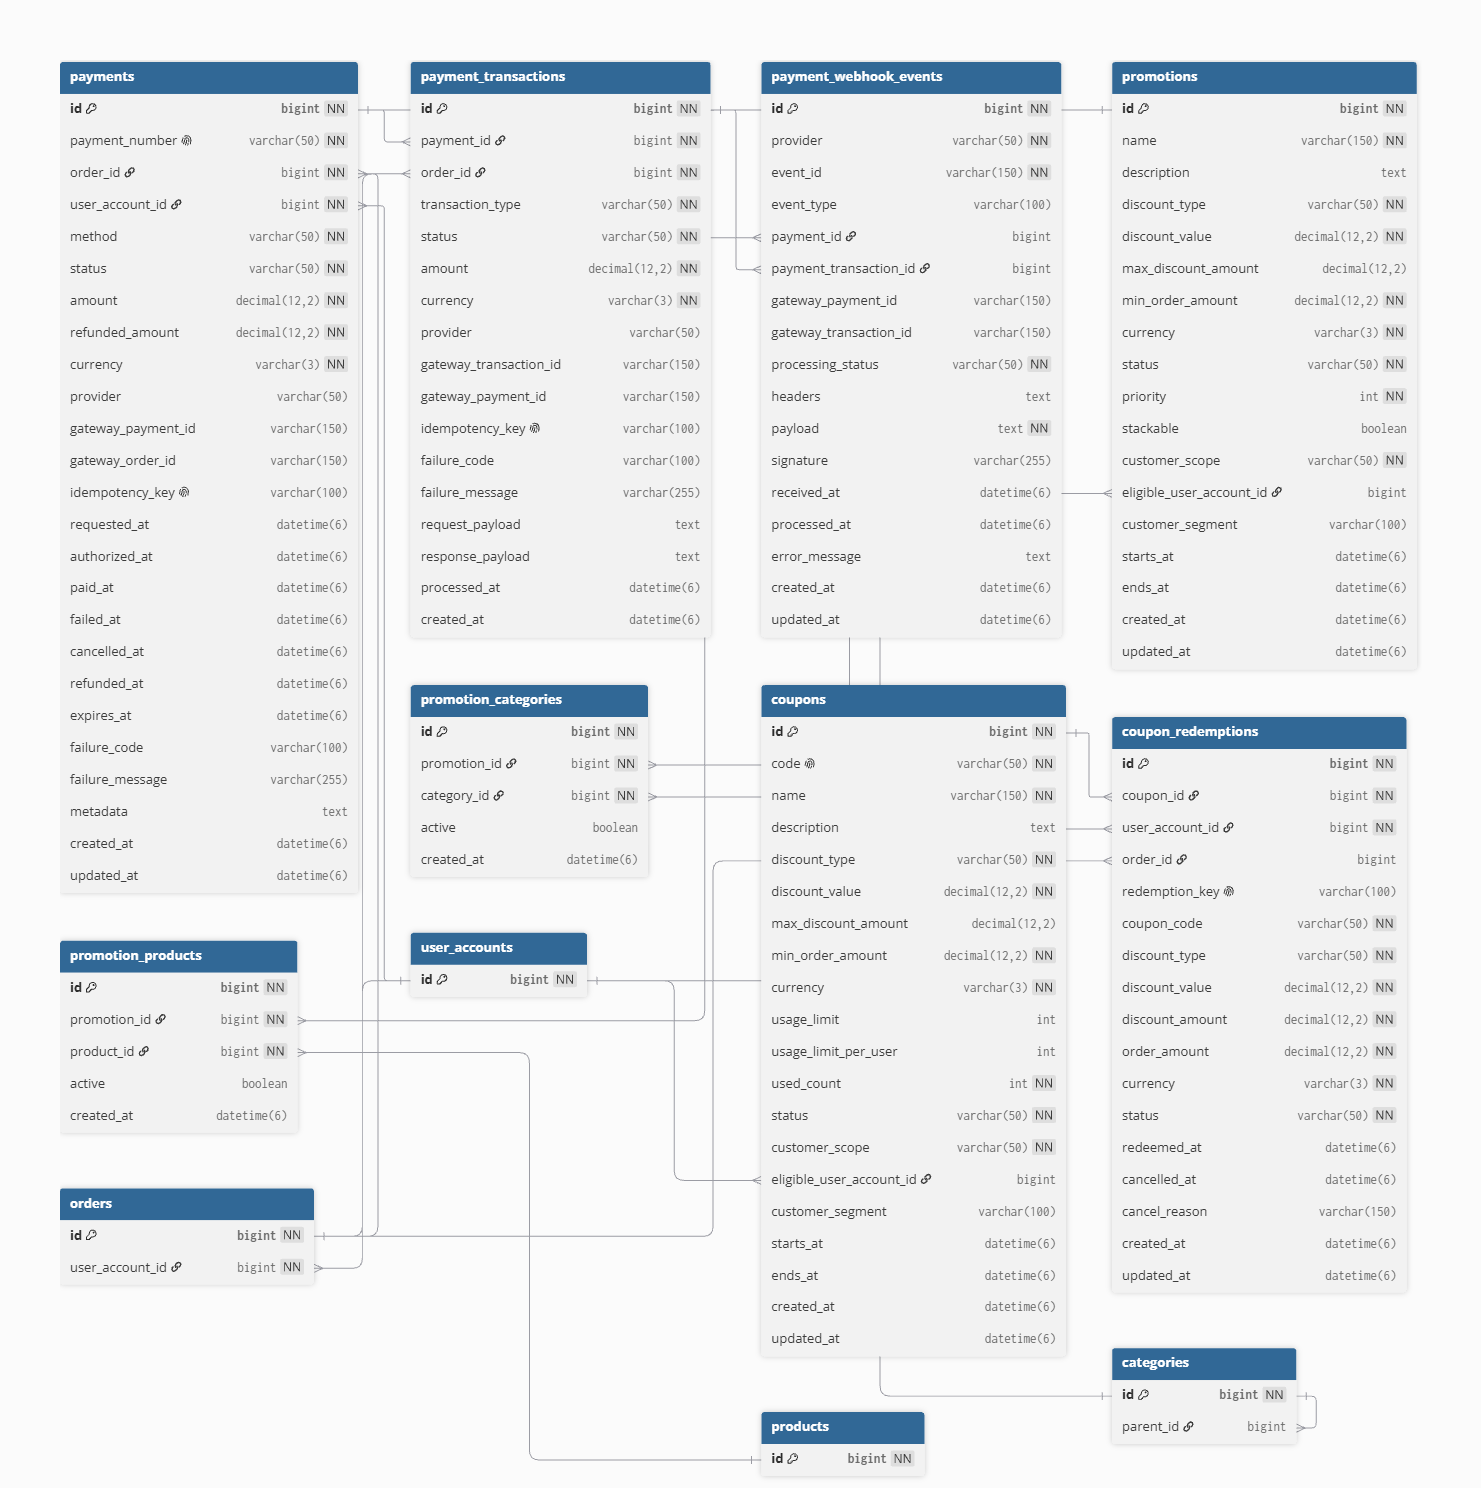
\includegraphics[
        width=\textwidth,
        height=0.72\textheight,
        keepaspectratio
    ]{Images/Thietkehethong/Thanh toán và khuyến mãi.png}
    \caption{Sơ đồ dữ liệu thanh toán và khuyến mãi}
    \label{fig:database-payment-promotion}
\end{figure}

Hình~\ref{fig:database-payment-promotion} thể hiện ba cụm quan hệ chính. Cụm
thanh toán liên kết \texttt{payments} với các lần giao dịch và sự kiện webhook
để hỗ trợ đối soát. Cụm khuyến mãi dùng các bảng liên kết để giới hạn phạm vi
theo sản phẩm hoặc danh mục. Cụm coupon ghi nhận lượt sử dụng theo người dùng và
đơn hàng, đồng thời chụp lại loại giảm, giá trị giảm và số tiền thực tế để bảo
toàn lịch sử tính giá.

Bảng~\ref{tab:data-summary-payment-promotion} tóm tắt chức năng của các bảng trong nhóm. Chỉ các bảng cốt lõi, đại diện trực tiếp cho luồng nghiệp vụ chính, được mô tả chi tiết trường dữ liệu.

\begin{longtable}{|>{\RaggedRight\arraybackslash}p{0.34\textwidth}|>{\RaggedRight\arraybackslash}p{0.56\textwidth}|}
    \caption{Các bảng thuộc nhóm thanh toán và khuyến mãi}
    \label{tab:data-summary-payment-promotion} \\
    \hline
    \textbf{Tên bảng} & \textbf{Chức năng} \\
    \hline
    \endfirsthead
    \multicolumn{2}{c}{\tablename\ \thetable\ (tiếp theo)} \\
    \hline
    \textbf{Tên bảng} & \textbf{Chức năng} \\
    \hline
    \endhead
    \texttt{payments} & Thanh toán. \\
    \hline
    \texttt{payment\_transactions} & Giao dịch thanh toán. \\
    \hline
    \texttt{payment\_webhook\_events} & Sự kiện webhook thanh toán. \\
    \hline
    \texttt{promotions} & Chương trình khuyến mãi. \\
    \hline
    \texttt{promotion\_products} & Sản phẩm áp dụng khuyến mãi. \\
    \hline
    \texttt{promotion\_categories} & Danh mục áp dụng khuyến mãi. \\
    \hline
    \texttt{coupons} & Mã giảm giá. \\
    \hline
    \texttt{coupon\_redemptions} & Lượt sử dụng mã giảm giá. \\
    \hline
\end{longtable}

\paragraph{Các bảng cốt lõi.}

\begin{longtable}{|>{\RaggedRight\arraybackslash}p{0.25\textwidth}|>{\RaggedRight\arraybackslash}p{0.20\textwidth}|>{\RaggedRight\arraybackslash}p{0.45\textwidth}|}
    \caption{Mô tả chi tiết bảng \texttt{payments} (Thanh toán)}
    \label{tab:data-dictionary-payments} \\
    \hline
    \textbf{Tên trường} & \textbf{Kiểu dữ liệu} & \textbf{Mô tả} \\
    \hline
    \endfirsthead
    \multicolumn{3}{c}{\tablename\ \thetable\ (tiếp theo)} \\
    \hline
    \textbf{Tên trường} & \textbf{Kiểu dữ liệu} & \textbf{Mô tả} \\
    \hline
    \endhead
    \texttt{\seqsplit{id}} & \texttt{bigint} & Khóa chính tự tăng. \\
        \hline
        \texttt{\seqsplit{payment\_number}} & \texttt{varchar(50)} & Mã thanh toán duy nhất; bắt buộc; duy nhất. \\
        \hline
        \texttt{\seqsplit{order\_id}} & \texttt{bigint} & Khóa ngoại tham chiếu \texttt{orders.id}; bắt buộc. \\
        \hline
        \texttt{\seqsplit{user\_account\_id}} & \texttt{bigint} & Khóa ngoại tham chiếu \texttt{user\_accounts.id}; bắt buộc. \\
        \hline
        \texttt{\seqsplit{method}} & \texttt{varchar(50)} & Phương thức thanh toán; bắt buộc. \\
        \hline
        \texttt{\seqsplit{status}} & \texttt{varchar(50)} & Trạng thái hiện tại; bắt buộc. \\
        \hline
        \texttt{\seqsplit{amount}} & \texttt{decimal(12,2)} & Số tiền; bắt buộc. \\
        \hline
        \texttt{\seqsplit{refunded\_amount}} & \texttt{decimal(12,2)} & Số tiền đã hoàn; bắt buộc. \\
        \hline
        \texttt{\seqsplit{currency}} & \texttt{varchar(3)} & Mã tiền tệ ISO 4217; bắt buộc. \\
        \hline
        \texttt{\seqsplit{provider}} & \texttt{varchar(50)} & Nhà cung cấp thanh toán. \\
        \hline
        \texttt{\seqsplit{gateway\_payment\_id}} & \texttt{varchar(150)} & Định danh thanh toán tại cổng. \\
        \hline
        \texttt{\seqsplit{gateway\_order\_id}} & \texttt{varchar(150)} & Định danh đơn hàng tại cổng. \\
        \hline
        \texttt{\seqsplit{idempotency\_key}} & \texttt{varchar(100)} & Khóa duy nhất chống xử lý lặp; duy nhất. \\
        \hline
        \texttt{\seqsplit{requested\_at}} & \texttt{datetime(6)} & Thời điểm yêu cầu thanh toán. \\
        \hline
        \texttt{\seqsplit{authorized\_at}} & \texttt{datetime(6)} & Thời điểm ủy quyền thanh toán. \\
        \hline
        \texttt{\seqsplit{paid\_at}} & \texttt{datetime(6)} & Thời điểm thanh toán thành công. \\
        \hline
        \texttt{\seqsplit{failed\_at}} & \texttt{datetime(6)} & Thời điểm thất bại. \\
        \hline
        \texttt{\seqsplit{cancelled\_at}} & \texttt{datetime(6)} & Thời điểm hủy. \\
        \hline
        \texttt{\seqsplit{refunded\_at}} & \texttt{datetime(6)} & Thời điểm hoàn tiền. \\
        \hline
        \texttt{\seqsplit{expires\_at}} & \texttt{datetime(6)} & Thời điểm hết hiệu lực. \\
        \hline
        \texttt{\seqsplit{failure\_code}} & \texttt{varchar(100)} & Mã lỗi. \\
        \hline
        \texttt{\seqsplit{failure\_message}} & \texttt{varchar(255)} & Thông báo lỗi. \\
        \hline
        \texttt{\seqsplit{metadata}} & \texttt{text} & Siêu dữ liệu bổ sung. \\
        \hline
        \texttt{\seqsplit{created\_at}} & \texttt{datetime(6)} & Thời điểm tạo bản ghi. \\
        \hline
        \texttt{\seqsplit{updated\_at}} & \texttt{datetime(6)} & Thời điểm cập nhật gần nhất. \\
        \hline
\end{longtable}

\begin{longtable}{|>{\RaggedRight\arraybackslash}p{0.25\textwidth}|>{\RaggedRight\arraybackslash}p{0.20\textwidth}|>{\RaggedRight\arraybackslash}p{0.45\textwidth}|}
    \caption{Mô tả chi tiết bảng \texttt{promotions} (Chương trình khuyến mãi)}
    \label{tab:data-dictionary-promotions} \\
    \hline
    \textbf{Tên trường} & \textbf{Kiểu dữ liệu} & \textbf{Mô tả} \\
    \hline
    \endfirsthead
    \multicolumn{3}{c}{\tablename\ \thetable\ (tiếp theo)} \\
    \hline
    \textbf{Tên trường} & \textbf{Kiểu dữ liệu} & \textbf{Mô tả} \\
    \hline
    \endhead
    \texttt{\seqsplit{id}} & \texttt{bigint} & Khóa chính tự tăng. \\
        \hline
        \texttt{\seqsplit{name}} & \texttt{varchar(150)} & Tên; bắt buộc. \\
        \hline
        \texttt{\seqsplit{description}} & \texttt{text} & Nội dung mô tả. \\
        \hline
        \texttt{\seqsplit{discount\_type}} & \texttt{varchar(50)} & Loại giảm giá; bắt buộc. \\
        \hline
        \texttt{\seqsplit{discount\_value}} & \texttt{decimal(12,2)} & Giá trị giảm giá; bắt buộc. \\
        \hline
        \texttt{\seqsplit{max\_discount\_amount}} & \texttt{decimal(12,2)} & Số tiền giảm tối đa. \\
        \hline
        \texttt{\seqsplit{min\_order\_amount}} & \texttt{decimal(12,2)} & Giá trị đơn hàng tối thiểu; bắt buộc. \\
        \hline
        \texttt{\seqsplit{currency}} & \texttt{varchar(3)} & Mã tiền tệ ISO 4217; bắt buộc. \\
        \hline
        \texttt{\seqsplit{status}} & \texttt{varchar(50)} & Trạng thái hiện tại; bắt buộc. \\
        \hline
        \texttt{\seqsplit{priority}} & \texttt{int} & Độ ưu tiên áp dụng; bắt buộc. \\
        \hline
        \texttt{\seqsplit{stackable}} & \texttt{boolean} & Cho biết có thể kết hợp với ưu đãi khác. \\
        \hline
        \texttt{\seqsplit{customer\_scope}} & \texttt{varchar(50)} & Phạm vi khách hàng áp dụng; bắt buộc. \\
        \hline
        \texttt{\seqsplit{eligible\_user\_account\_id}} & \texttt{bigint} & Khóa ngoại tham chiếu \texttt{user\_accounts.id}. \\
        \hline
        \texttt{\seqsplit{customer\_segment}} & \texttt{varchar(100)} & Phân khúc khách hàng. \\
        \hline
        \texttt{\seqsplit{starts\_at}} & \texttt{datetime(6)} & Thời điểm bắt đầu hiệu lực. \\
        \hline
        \texttt{\seqsplit{ends\_at}} & \texttt{datetime(6)} & Thời điểm kết thúc hiệu lực. \\
        \hline
        \texttt{\seqsplit{created\_at}} & \texttt{datetime(6)} & Thời điểm tạo bản ghi. \\
        \hline
        \texttt{\seqsplit{updated\_at}} & \texttt{datetime(6)} & Thời điểm cập nhật gần nhất. \\
        \hline
\end{longtable}



\subsubsection{Nhóm dữ liệu tích hợp và đồng bộ AI}

Nhóm tích hợp AI lưu trạng thái các công việc đồng bộ, mốc đồng bộ thành công gần
nhất và dữ liệu hội thoại của trợ lý. Phiên, tin nhắn, sản phẩm được gợi ý và phản
hồi của người dùng được tách riêng để hỗ trợ hội thoại nhiều lượt, đánh giá chất
lượng kết quả và truy vết sản phẩm đã được AI sử dụng trong câu trả lời.

\begin{figure}[H]
    \centering
    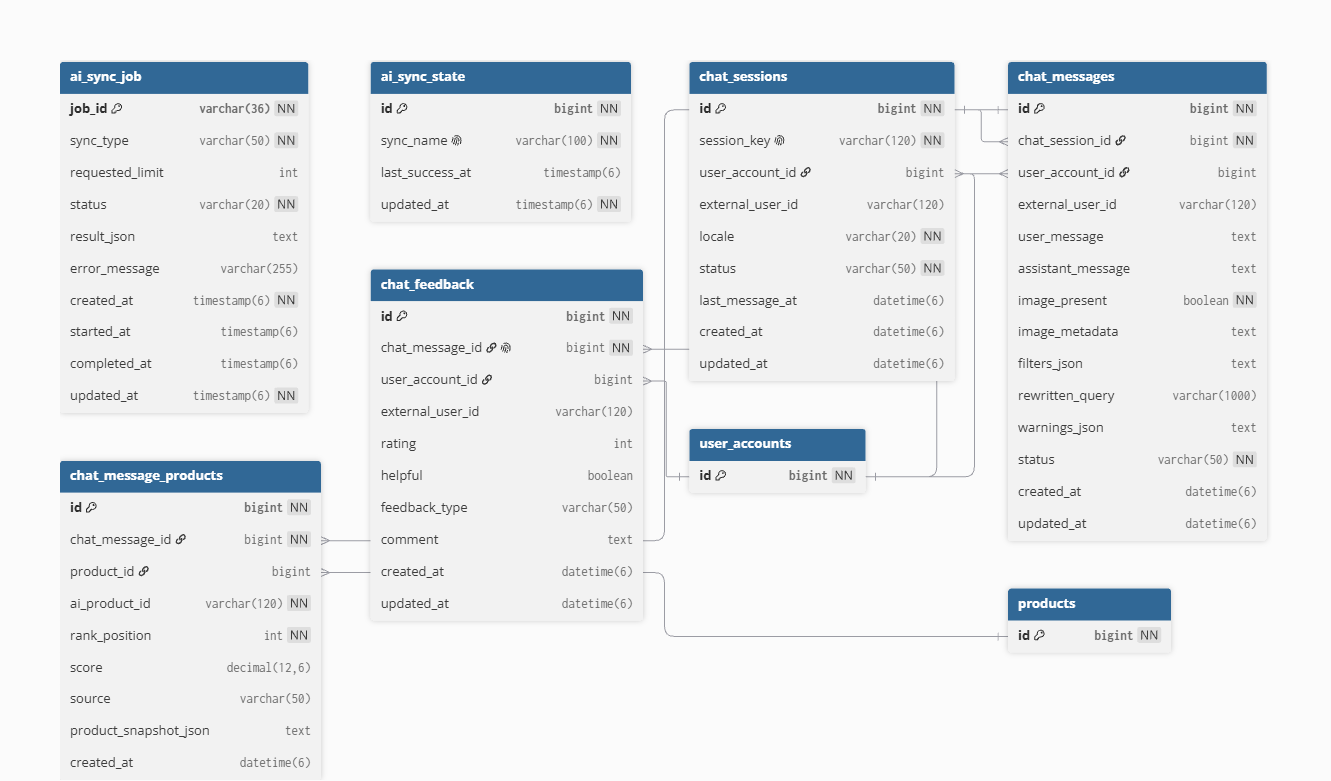
\includegraphics[
        width=\textwidth,
        height=0.72\textheight,
        keepaspectratio
    ]{Images/Thietkehethong/Tích hợp và đồng bộ AI.png}
    \caption{Sơ đồ dữ liệu tích hợp và đồng bộ AI}
    \label{fig:database-ai-integration}
\end{figure}

Theo Hình~\ref{fig:database-ai-integration}, một phiên hội thoại gồm nhiều tin
nhắn; mỗi tin nhắn có thể gắn với các sản phẩm được AI đề xuất và tối đa một phản
hồi đánh giá. Liên kết đến tài khoản và sản phẩm có thể rỗng để hỗ trợ khách chưa
đăng nhập cũng như bảo toàn bản chụp kết quả AI. Hai bảng
\texttt{ai\_sync\_job} và \texttt{ai\_sync\_state} không có khóa ngoại với
cụm hội thoại vì chúng theo dõi tiến trình lập chỉ mục ở cấp hệ thống, thay vì
biểu diễn một lượt tương tác của người dùng.

Bảng~\ref{tab:data-summary-ai-integration} tóm tắt chức năng của các bảng trong nhóm. Chỉ các bảng cốt lõi, đại diện trực tiếp cho luồng nghiệp vụ chính, được mô tả chi tiết trường dữ liệu.

\begin{longtable}{|>{\RaggedRight\arraybackslash}p{0.34\textwidth}|>{\RaggedRight\arraybackslash}p{0.56\textwidth}|}
    \caption{Các bảng thuộc nhóm tích hợp và đồng bộ AI}
    \label{tab:data-summary-ai-integration} \\
    \hline
    \textbf{Tên bảng} & \textbf{Chức năng} \\
    \hline
    \endfirsthead
    \multicolumn{2}{c}{\tablename\ \thetable\ (tiếp theo)} \\
    \hline
    \textbf{Tên bảng} & \textbf{Chức năng} \\
    \hline
    \endhead
    \texttt{ai\_sync\_job} & Công việc đồng bộ AI. \\
    \hline
    \texttt{ai\_sync\_state} & Trạng thái đồng bộ AI. \\
    \hline
    \texttt{chat\_sessions} & Phiên hội thoại. \\
    \hline
    \texttt{chat\_messages} & Tin nhắn hội thoại. \\
    \hline
    \texttt{chat\_message\_products} & Sản phẩm trong câu trả lời. \\
    \hline
    \texttt{chat\_feedback} & Phản hồi hội thoại. \\
    \hline
\end{longtable}

\paragraph{Các bảng cốt lõi.}

\begin{longtable}{|>{\RaggedRight\arraybackslash}p{0.25\textwidth}|>{\RaggedRight\arraybackslash}p{0.20\textwidth}|>{\RaggedRight\arraybackslash}p{0.45\textwidth}|}
    \caption{Mô tả chi tiết bảng \texttt{ai\_sync\_job} (Công việc đồng bộ AI)}
    \label{tab:data-dictionary-ai-sync-job} \\
    \hline
    \textbf{Tên trường} & \textbf{Kiểu dữ liệu} & \textbf{Mô tả} \\
    \hline
    \endfirsthead
    \multicolumn{3}{c}{\tablename\ \thetable\ (tiếp theo)} \\
    \hline
    \textbf{Tên trường} & \textbf{Kiểu dữ liệu} & \textbf{Mô tả} \\
    \hline
    \endhead
    \texttt{\seqsplit{job\_id}} & \texttt{varchar(36)} & Khóa chính. \\
        \hline
        \texttt{\seqsplit{sync\_type}} & \texttt{varchar(50)} & Loại tác vụ đồng bộ; bắt buộc. \\
        \hline
        \texttt{\seqsplit{requested\_limit}} & \texttt{int} & Số lượng bản ghi tối đa được yêu cầu xử lý. \\
        \hline
        \texttt{\seqsplit{status}} & \texttt{varchar(20)} & Trạng thái hiện tại; bắt buộc. \\
        \hline
        \texttt{\seqsplit{result\_json}} & \texttt{text} & Kết quả tác vụ ở định dạng JSON. \\
        \hline
        \texttt{\seqsplit{error\_message}} & \texttt{varchar(255)} & Thông báo lỗi khi xử lý. \\
        \hline
        \texttt{\seqsplit{created\_at}} & \texttt{timestamp(6)} & Thời điểm tạo bản ghi; bắt buộc. \\
        \hline
        \texttt{\seqsplit{started\_at}} & \texttt{timestamp(6)} & Thời điểm bắt đầu xử lý. \\
        \hline
        \texttt{\seqsplit{completed\_at}} & \texttt{timestamp(6)} & Thời điểm hoàn tất xử lý. \\
        \hline
        \texttt{\seqsplit{updated\_at}} & \texttt{timestamp(6)} & Thời điểm cập nhật gần nhất; bắt buộc. \\
        \hline
\end{longtable}

\begin{longtable}{|>{\RaggedRight\arraybackslash}p{0.25\textwidth}|>{\RaggedRight\arraybackslash}p{0.20\textwidth}|>{\RaggedRight\arraybackslash}p{0.45\textwidth}|}
    \caption{Mô tả chi tiết bảng \texttt{chat\_sessions} (Phiên hội thoại)}
    \label{tab:data-dictionary-chat-sessions} \\
    \hline
    \textbf{Tên trường} & \textbf{Kiểu dữ liệu} & \textbf{Mô tả} \\
    \hline
    \endfirsthead
    \multicolumn{3}{c}{\tablename\ \thetable\ (tiếp theo)} \\
    \hline
    \textbf{Tên trường} & \textbf{Kiểu dữ liệu} & \textbf{Mô tả} \\
    \hline
    \endhead
    \texttt{\seqsplit{id}} & \texttt{bigint} & Khóa chính tự tăng. \\
        \hline
        \texttt{\seqsplit{session\_key}} & \texttt{varchar(120)} & Khóa duy nhất của phiên hội thoại; bắt buộc; duy nhất. \\
        \hline
        \texttt{\seqsplit{user\_account\_id}} & \texttt{bigint} & Khóa ngoại tham chiếu \texttt{user\_accounts.id}. \\
        \hline
        \texttt{\seqsplit{external\_user\_id}} & \texttt{varchar(120)} & Định danh khách chưa đăng nhập. \\
        \hline
        \texttt{\seqsplit{locale}} & \texttt{varchar(20)} & Ngôn ngữ của phiên; bắt buộc. \\
        \hline
        \texttt{\seqsplit{status}} & \texttt{varchar(50)} & Trạng thái hiện tại; bắt buộc. \\
        \hline
        \texttt{\seqsplit{last\_message\_at}} & \texttt{datetime(6)} & Thời điểm có tin nhắn gần nhất. \\
        \hline
        \texttt{\seqsplit{created\_at}} & \texttt{datetime(6)} & Thời điểm tạo bản ghi. \\
        \hline
        \texttt{\seqsplit{updated\_at}} & \texttt{datetime(6)} & Thời điểm cập nhật gần nhất. \\
        \hline
\end{longtable}

\begin{longtable}{|>{\RaggedRight\arraybackslash}p{0.25\textwidth}|>{\RaggedRight\arraybackslash}p{0.20\textwidth}|>{\RaggedRight\arraybackslash}p{0.45\textwidth}|}
    \caption{Mô tả chi tiết bảng \texttt{chat\_messages} (Tin nhắn hội thoại)}
    \label{tab:data-dictionary-chat-messages} \\
    \hline
    \textbf{Tên trường} & \textbf{Kiểu dữ liệu} & \textbf{Mô tả} \\
    \hline
    \endfirsthead
    \multicolumn{3}{c}{\tablename\ \thetable\ (tiếp theo)} \\
    \hline
    \textbf{Tên trường} & \textbf{Kiểu dữ liệu} & \textbf{Mô tả} \\
    \hline
    \endhead
    \texttt{\seqsplit{id}} & \texttt{bigint} & Khóa chính tự tăng. \\
        \hline
        \texttt{\seqsplit{chat\_session\_id}} & \texttt{bigint} & Khóa ngoại tham chiếu \texttt{chat\_sessions.id}; bắt buộc. \\
        \hline
        \texttt{\seqsplit{user\_account\_id}} & \texttt{bigint} & Khóa ngoại tham chiếu \texttt{user\_accounts.id}. \\
        \hline
        \texttt{\seqsplit{external\_user\_id}} & \texttt{varchar(120)} & Định danh khách chưa đăng nhập. \\
        \hline
        \texttt{\seqsplit{user\_message}} & \texttt{text} & Nội dung người dùng gửi. \\
        \hline
        \texttt{\seqsplit{assistant\_message}} & \texttt{text} & Nội dung trợ lý trả lời. \\
        \hline
        \texttt{\seqsplit{image\_present}} & \texttt{boolean} & Cho biết yêu cầu có kèm hình ảnh; bắt buộc. \\
        \hline
        \texttt{\seqsplit{image\_metadata}} & \texttt{text} & Siêu dữ liệu của hình ảnh. \\
        \hline
        \texttt{\seqsplit{filters\_json}} & \texttt{text} & Bộ lọc tìm kiếm ở định dạng JSON. \\
        \hline
        \texttt{\seqsplit{rewritten\_query}} & \texttt{varchar(1000)} & Truy vấn đã được AI viết lại. \\
        \hline
        \texttt{\seqsplit{warnings\_json}} & \texttt{text} & Danh sách cảnh báo ở định dạng JSON. \\
        \hline
        \texttt{\seqsplit{status}} & \texttt{varchar(50)} & Trạng thái hiện tại; bắt buộc. \\
        \hline
        \texttt{\seqsplit{created\_at}} & \texttt{datetime(6)} & Thời điểm tạo bản ghi. \\
        \hline
        \texttt{\seqsplit{updated\_at}} & \texttt{datetime(6)} & Thời điểm cập nhật gần nhất. \\
        \hline
\end{longtable}



\subsubsection{Thiết kế chỉ mục và đồng bộ dữ liệu MySQL--Qdrant}

MySQL là nguồn dữ liệu chuẩn, còn Qdrant chỉ lưu dữ liệu dẫn xuất phục vụ truy hồi. Mỗi điểm trong chỉ mục sử dụng \texttt{product\_id} làm khóa liên kết ổn định với sản phẩm trong MySQL. Vector văn bản và vector hình ảnh có thể được tổ chức trong các collection riêng do khác nhau về mô hình embedding, số chiều và chiến lược truy vấn. Payload chỉ chứa metadata cần thiết cho lọc và xếp hạng, chẳng hạn danh mục, thuộc tính, khoảng giá, trạng thái khả dụng và thời điểm cập nhật.

Giá, tồn kho và trạng thái trong payload là ảnh chụp tại thời điểm lập chỉ mục nên có thể chậm hơn dữ liệu nghiệp vụ. Vì vậy, Qdrant chỉ được dùng để tìm tập ứng viên; Spring Boot luôn nạp lại sản phẩm từ MySQL, loại các bản ghi không còn hợp lệ và sử dụng giá cùng tồn kho hiện hành trước khi trả kết quả cho Frontend.

Hệ thống hỗ trợ đồng bộ toàn bộ, đồng bộ tăng dần, đồng bộ một sản phẩm và xóa sản phẩm khỏi chỉ mục. Spring Boot tạo DTO lập chỉ mục từ dữ liệu MySQL; AI Service tạo embedding, xây dựng payload rồi thực hiện upsert hoặc delete trong Qdrant. Các thao tác dùng \texttt{product\_id} ổn định nên có thể thực hiện lại an toàn khi gặp lỗi tạm thời.

\begin{figure}[H]
    \centering
    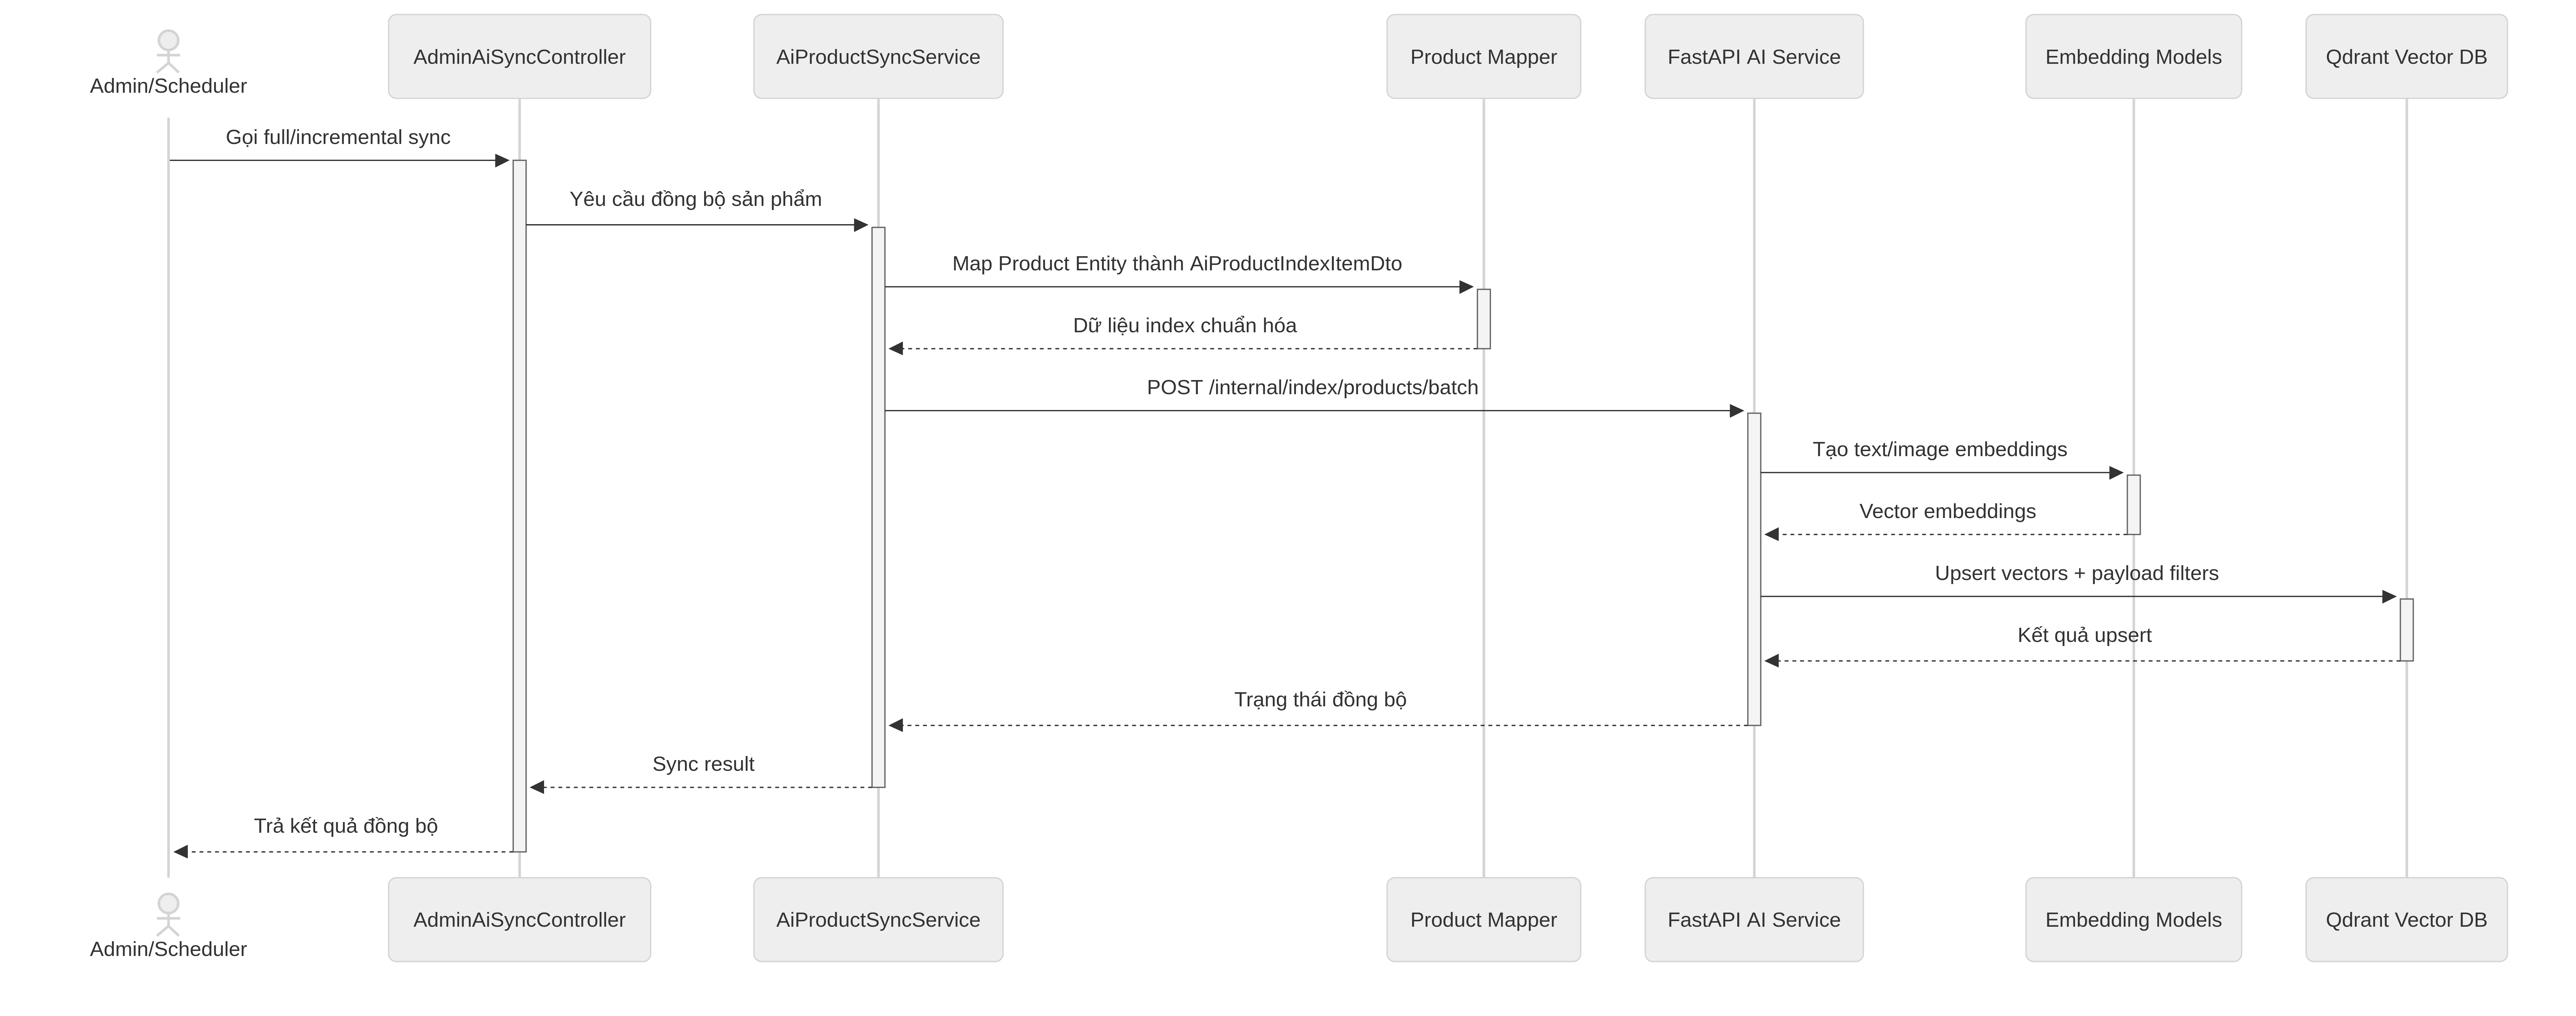
\includegraphics[width=0.95\textwidth]{Images/Thietkehethong/dongboAI.png}
    \caption{Luồng đồng bộ dữ liệu từ MySQL sang Qdrant}
    \label{fig:ai-sync-flow}
\end{figure}

Tiến trình được ghi nhận trong \texttt{ai\_sync\_job}, còn \texttt{ai\_sync\_state} lưu mốc đồng bộ thành công gần nhất. Một công việc có thể hoàn thành toàn bộ, thất bại hoặc thành công một phần; kết quả cần ghi số bản ghi thành công, số bản ghi lỗi và các mã sản phẩm cần thử lại. Lỗi cập nhật Qdrant không hoàn tác giao dịch nghiệp vụ trong MySQL vì chỉ mục có thể được tái tạo.

\subsection{Thiết kế các chức năng chính}

Các activity diagram của các luồng chính đã được trình bày tại Chương 5. Phần này không lặp lại luồng điều khiển giữa các tác nhân mà tập trung vào quyết định thiết kế bên trong: quy tắc kiểm tra, ranh giới transaction, chuyển trạng thái, dữ liệu đầu ra và phương án suy giảm khi một phụ thuộc không khả dụng.

\subsubsection{Checkout và quản lý vòng đời đơn hàng}

Hai thao tác preview và confirm được tách riêng. Preview là phép đọc để tính giá dự kiến, giảm giá tự động và coupon; thao tác này không tạo đơn hay giữ tồn kho. Confirm thực hiện lại toàn bộ kiểm tra trong transaction: giỏ và địa chỉ thuộc người dùng, sản phẩm còn bán, biến thể đủ số lượng, giá còn hiệu lực và coupon còn áp dụng.

Khi các điều kiện hợp lệ, Backend tạo \texttt{Order}, chụp lại địa chỉ và thông tin từng dòng hàng, áp dụng coupon, giữ tồn kho, tạo lịch sử trạng thái rồi chuyển giỏ sang \texttt{CHECKED\_OUT}. Bất kỳ lỗi nào trong chuỗi ghi bắt buộc đều làm rollback transaction. Luồng đặt hàng COD được thể hiện tại Hình~\ref{fig:activity-cod-checkout}; phần xác nhận và cập nhật trạng thái COD được thể hiện tại Hình~\ref{fig:activity-cod-confirmation}.

Trạng thái đơn hàng được quản lý bằng một tập chuyển tiếp hữu hạn. Mỗi lệnh phải kiểm tra trạng thái nguồn, vai trò người thực hiện và tác động kèm theo đối với tồn kho hoặc thanh toán. Lịch sử trạng thái được ghi bất biến để truy vết; không cập nhật trực tiếp trạng thái đơn mà bỏ qua service nghiệp vụ.

\begin{figure}[H]
    \centering
    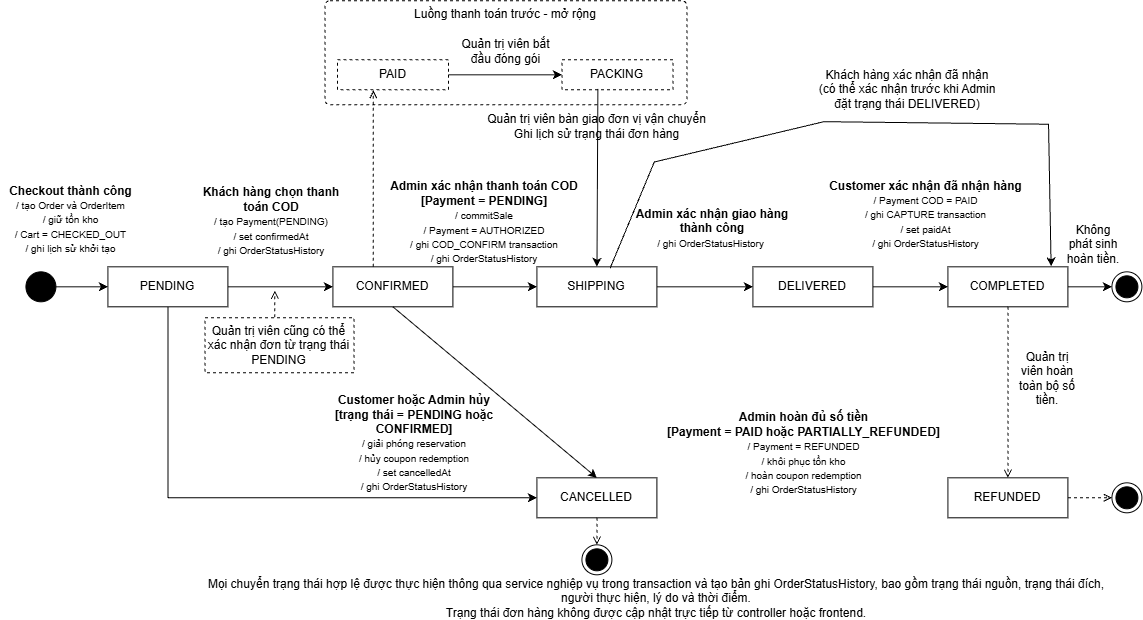
\includegraphics[width=0.98\textwidth]{Images/Thietkehethong/Thiết kế vòng đời trạng thái đơn hàng và các tác động nghiệp vụ.drawio.png}
    \caption{Thiết kế vòng đời trạng thái đơn hàng và các tác động nghiệp vụ}
    \label{fig:order-state-design}
\end{figure}

Hình~\ref{fig:order-state-design} phân biệt luồng COD đang được sử dụng với nhánh thanh toán trước dự kiến mở rộng. Trong luồng COD, đơn được tạo ở trạng thái \texttt{PENDING}, chuyển sang \texttt{CONFIRMED} sau khi phương thức thanh toán được xác lập, rồi sang \texttt{SHIPPING} khi quản trị viên xác nhận khoản COD và bàn giao vận chuyển. Quản trị viên có thể đánh dấu giao hàng thành công để chuyển đơn sang \texttt{DELIVERED}; khách hàng xác nhận đã nhận hàng từ \texttt{SHIPPING} hoặc \texttt{DELIVERED} để hoàn tất đơn. Tại thời điểm đó, khoản COD được ghi nhận là đã thanh toán và transaction thu tiền được lưu để đối soát.

Đơn chỉ được hủy từ \texttt{PENDING} hoặc \texttt{CONFIRMED}. Thao tác hủy giải phóng phần tồn kho đã giữ, hoàn lượt sử dụng coupon và ghi lịch sử chuyển trạng thái. Đối với đơn đã hoàn thành, hoàn đủ số tiền chuyển đơn sang \texttt{REFUNDED}, đồng thời khôi phục tồn kho và coupon theo transaction hoàn tiền. Nhánh \texttt{PAID}--\texttt{PACKING} được biểu diễn bằng nét đứt để thể hiện khả năng tích hợp thanh toán trước mà không làm thay đổi luồng COD hiện hành. Mọi chuyển tiếp hợp lệ đều đi qua service nghiệp vụ trong transaction và sinh bản ghi \texttt{OrderStatusHistory}; controller không được cập nhật trực tiếp trạng thái đơn hàng.

\subsubsection{Tìm kiếm sản phẩm bằng AI}

Luồng tương tác đa phương thức đã được mô tả tại Hình~\ref{fig:activity-multimodal-search}. Về thiết kế xử lý, request được quy về một mô hình chung gồm truy vấn văn bản tùy chọn, ảnh tùy chọn, vùng quan tâm, bộ lọc và giới hạn kết quả. Endpoint \texttt{auto} lựa chọn nhánh phù hợp theo dữ liệu thực nhận; endpoint chuyên biệt từ chối request thiếu đầu vào bắt buộc.

Pipeline gồm bốn giai đoạn. Thứ nhất, Query Understanding chuẩn hóa truy vấn và sinh bộ lọc có cấu trúc. Thứ hai, ảnh được kiểm tra và cắt theo vùng người dùng chọn hoặc vùng YOLO phát hiện; YOLO không phải phụ thuộc bắt buộc. Thứ ba, embedding provider tạo vector cùng không gian với collection Qdrant. Cuối cùng, Search Service truy hồi tập ứng viên, áp dụng filter và tùy chọn reranking.

Kết quả AI chỉ chứa \texttt{product\_id}, điểm số, nguồn truy hồi và cảnh báo. \texttt{ProductCardResolver} tại Spring Boot nạp lại dữ liệu hiện hành từ MySQL, loại ứng viên không hợp lệ và bảo toàn thứ tự còn lại. Khi AI Service lỗi và request có truy vấn văn bản, Backend có thể dùng keyword fallback; nếu chỉ có ảnh, hệ thống trả trạng thái suy giảm rõ ràng thay vì tạo kết quả không có căn cứ.

\begin{figure}[H]
    \centering
    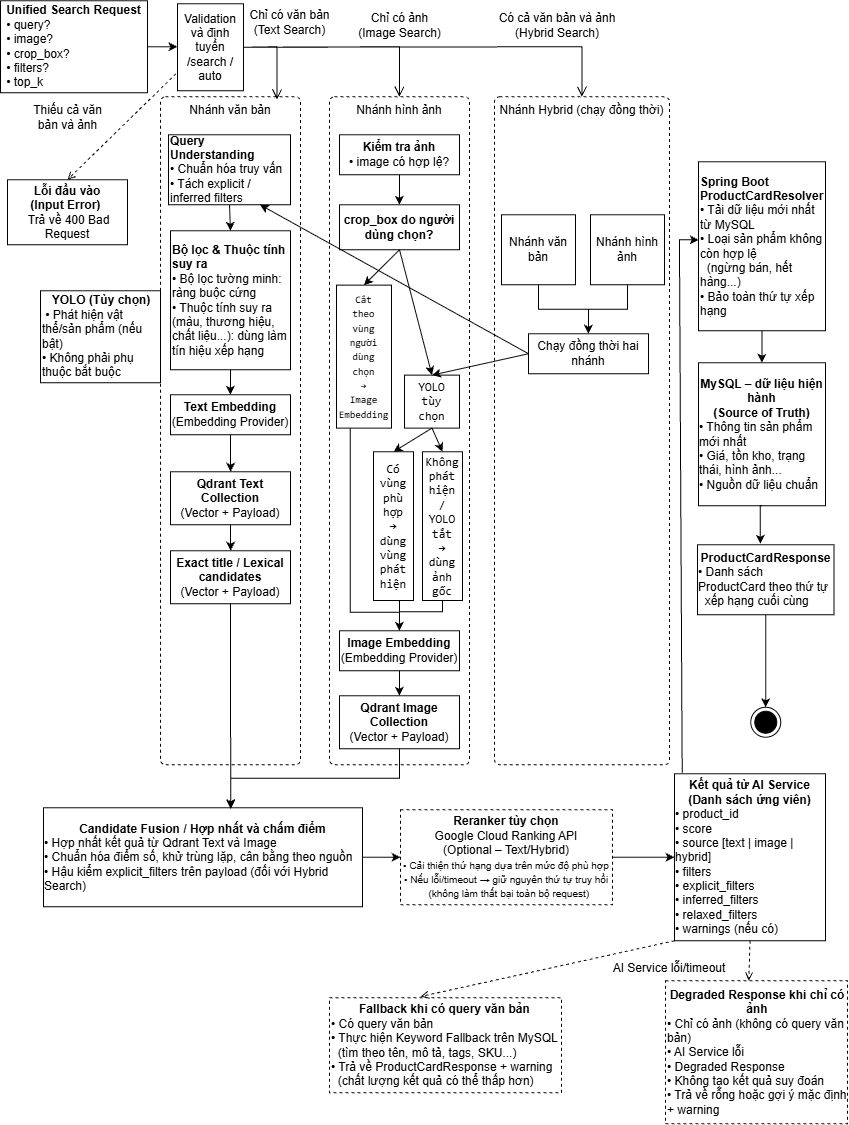
\includegraphics[width=0.92\textwidth,height=0.78\textheight,keepaspectratio]{Images/Thietkehethong/Pipeline xử lý tìm kiếm sản phẩm đa phương thức.drawio.png}
    \caption{Pipeline xử lý tìm kiếm sản phẩm đa phương thức}
    \label{fig:ai-search-pipeline}
\end{figure}

Hình~\ref{fig:ai-search-pipeline} mô tả cách endpoint \texttt{/search/auto} kiểm tra request và định tuyến theo dữ liệu đầu vào. Với truy vấn văn bản, Query Understanding chuẩn hóa câu truy vấn, phân biệt bộ lọc tường minh với thuộc tính suy ra và tạo text embedding. Tập ứng viên vector từ Qdrant được kết hợp với ứng viên khớp tên hoặc lexical khi chức năng này được bật. Với truy vấn ảnh, vùng \texttt{crop\_box} do người dùng chọn được ưu tiên và đưa thẳng đến bước embedding; nếu không có vùng chọn, hệ thống có thể dùng YOLO để phát hiện đối tượng, đồng thời quay về ảnh gốc khi YOLO bị tắt hoặc không tìm được vùng phù hợp.

Tìm kiếm kết hợp thực thi đồng thời nhánh văn bản và nhánh ảnh, sau đó hợp nhất ứng viên, khử trùng lặp, cân bằng điểm theo nguồn và hậu kiểm các ràng buộc tường minh trên payload. Reranker là bước tùy chọn cho tìm kiếm văn bản và kết hợp; lỗi hoặc timeout tại bước này không làm mất kết quả truy hồi ban đầu. AI Service chỉ trả định danh sản phẩm, điểm số, nguồn và thông tin bộ lọc. Spring Boot dùng \texttt{ProductCardResolver} để nạp dữ liệu hiện hành từ MySQL, loại sản phẩm không còn hợp lệ và bảo toàn thứ tự xếp hạng trước khi tạo \texttt{ProductCardResponse}. Khi AI Service không khả dụng, request có văn bản được chuyển sang keyword fallback trên MySQL; request chỉ có ảnh nhận response suy giảm rõ ràng thay vì kết quả suy đoán.

\subsubsection{Trợ lý hội thoại}

\begin{figure}[H]
    \centering
    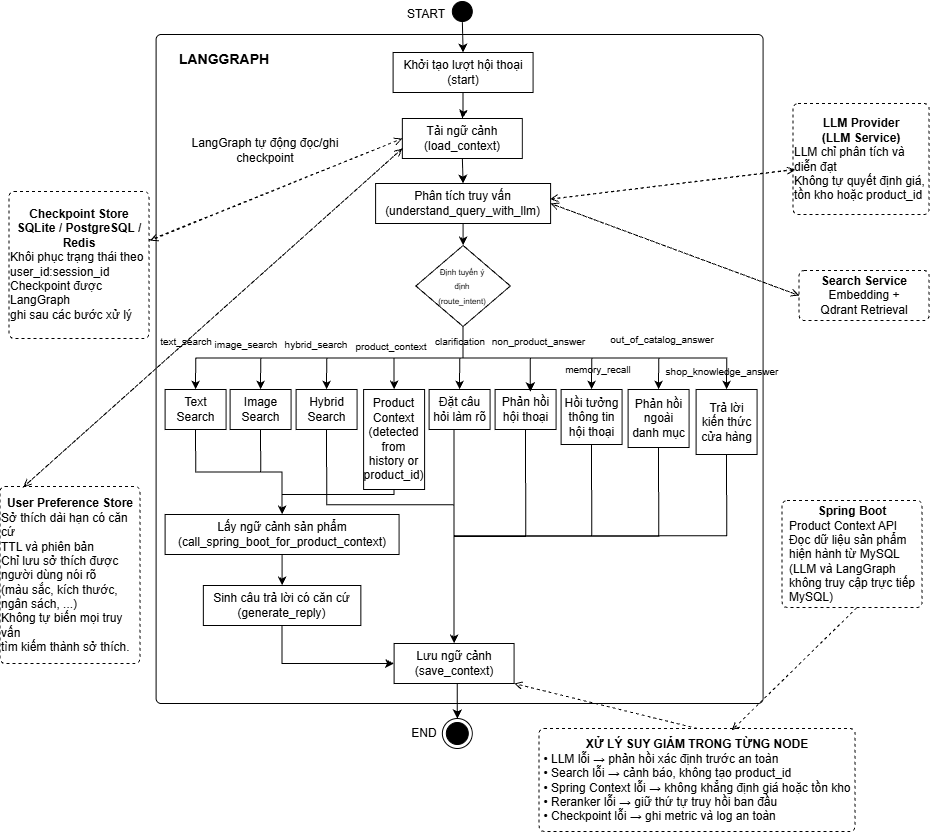
\includegraphics[width=0.96\textwidth,height=0.80\textheight,keepaspectratio]{Images/Thietkehethong/Thiết kế đồ thị trạng thái của trợ lý hội thoại.drawio.png}
    \caption{Thiết kế đồ thị trạng thái của trợ lý hội thoại}
    \label{fig:assistant-state-graph}
\end{figure}

Luồng tương tác giữa người dùng, Backend và AI Service đã được trình bày tại Hình~\ref{fig:activity-multiturn-chat}. Hình~\ref{fig:assistant-state-graph} tập trung vào cách AI Service điều phối một lượt hội thoại bằng đồ thị trạng thái LangGraph. Trạng thái dùng chung mang định danh phiên, lịch sử hội thoại đã rút gọn, sở thích người dùng có căn cứ, kết quả phân tích truy vấn, tập ứng viên sản phẩm và các cảnh báo phát sinh. Cách tổ chức này cho phép từng nút chỉ đọc và cập nhật phần dữ liệu cần thiết, đồng thời duy trì ngữ cảnh nhất quán giữa các lượt trao đổi.

Mỗi lượt xử lý bắt đầu tại nút \texttt{start}, sau đó \texttt{load\_context} nạp checkpoint và thông tin sở thích liên quan. Nút \texttt{understand\_query\_with\_llm} phân tích nội dung đầu vào; \texttt{route\_intent} sử dụng kết quả này để chọn nhánh xử lý. Truy vấn sản phẩm được định tuyến đến tìm kiếm văn bản, tìm kiếm ảnh hoặc tìm kiếm kết hợp. Kết quả tìm kiếm chỉ chứa tập ứng viên và được chuyển đến \texttt{call\_spring\_boot\_for\_product\_context} để lấy dữ liệu sản phẩm hiện hành trước khi \texttt{generate\_reply} sinh câu trả lời. Nếu truy vấn đã chứa đủ tham chiếu đến sản phẩm trong ngữ cảnh hội thoại, workflow có thể đi thẳng đến bước lấy ngữ cảnh sản phẩm mà không thực hiện một lượt tìm kiếm mới.

Các ý định không yêu cầu truy hồi sản phẩm được tách thành những nhánh riêng: đặt câu hỏi làm rõ, phản hồi hội thoại thông thường, hồi tưởng thông tin đã được ghi nhận, phản hồi truy vấn ngoài danh mục và trả lời kiến thức cửa hàng. Việc tách nhánh giúp áp dụng chỉ dẫn và giới hạn dữ liệu phù hợp cho từng loại câu trả lời, thay vì sử dụng một prompt chung cho mọi tình huống. Dù đi qua nhánh nào, kết quả cuối cùng đều hội tụ tại \texttt{save\_context} trước khi kết thúc lượt xử lý, nhờ đó trạng thái mới có thể được dùng cho câu hỏi tiếp theo.

Các khối nằm ngoài biên LangGraph thể hiện phụ thuộc tích hợp, không phải trạng thái nghiệp vụ. LLM Provider hỗ trợ phân tích truy vấn và sinh ngôn ngữ; Search Service thực hiện truy hồi ứng viên; Spring Boot Product Context API cung cấp dữ liệu chuẩn về sản phẩm. Checkpoint Store lưu trạng thái thực thi theo phiên, trong khi User Preference Store chỉ lưu những sở thích đủ căn cứ để tái sử dụng. Trợ lý không truy cập trực tiếp MySQL và không xem dữ liệu trong chỉ mục tìm kiếm là nguồn sự thật cuối cùng.

Thiết kế cũng quy định cơ chế suy giảm tại từng điểm phụ thuộc. Khi reranker gặp lỗi, hệ thống giữ thứ tự truy hồi ban đầu; khi Search Service không khả dụng, workflow không tự tạo định danh sản phẩm; và khi không lấy được ngữ cảnh từ Spring Boot, câu trả lời không khẳng định giá hoặc tồn kho. Lỗi mô hình được chuyển thành phản hồi an toàn, còn lỗi checkpoint được ghi nhận qua log và metric để phục vụ giám sát. Nhờ vậy, sự cố của một thành phần AI không làm phát sinh thông tin giao dịch không có căn cứ.

\subsection{Thiết kế giao tiếp và tích hợp}

\subsubsection{Hợp đồng giao tiếp giữa các dịch vụ}

Frontend chỉ gọi API công khai của Spring Boot. Backend tiếp nhận danh tính người dùng, kiểm tra quyền và điều phối nghiệp vụ trước khi gọi AI Service qua API nội bộ. AI Service có thể đọc ngữ cảnh giới hạn từ Spring Boot nhưng không truy cập trực tiếp MySQL. API quản trị dùng tiền tố \texttt{/admin}, còn endpoint tích hợp giữa hai dịch vụ dùng \texttt{/internal}.

Request và response thông thường sử dụng JSON; dữ liệu ảnh tuân theo hợp đồng của endpoint tìm kiếm tương ứng. DTO xác định rõ trường bắt buộc, giới hạn dữ liệu và cấu trúc lồng nhau. Spring Boot không truyền JPA Entity sang AI Service mà chuyển sản phẩm thành indexing DTO dạng \texttt{snake\_case}.

Luồng lập chỉ mục được khởi tạo qua các API quản trị \texttt{POST} \path{/admin/ai-sync/full}, \path{/admin/ai-sync/incremental} và \path{/admin/ai-sync/products/\{productId\}}. Tại ranh giới nội bộ, AI Service cung cấp \texttt{POST} \path{/internal/index/products/batch}, \texttt{POST} \path{/internal/index/products/\{product_id\}} và \texttt{DELETE} \path{/internal/index/products/\{product_id\}}. Các endpoint ghi chỉ mục sử dụng định danh sản phẩm ổn định để hỗ trợ gọi lại an toàn.

Indexing DTO chứa định danh, nội dung mô tả, phân loại, thuộc tính biến thể, giá hiệu lực, tổng tồn, trạng thái khả dụng, URL ảnh và thời điểm cập nhật. \texttt{product\_id} là khóa liên kết ổn định giữa MySQL và Qdrant.

AI Service dùng DTO để tạo nội dung embedding và payload Qdrant nhưng không trả payload đó trực tiếp cho Frontend. Search response chỉ cần định danh ứng viên, điểm số, nguồn truy hồi, bộ lọc đã áp dụng và cảnh báo. Assistant response bổ sung nội dung trả lời, mã phiên và danh sách định danh sản phẩm có căn cứ.

\begin{table}[H]
    \centering
    \caption{Các hợp đồng chính giữa Spring Boot và AI Service}
    \label{tab:spring-ai-contracts}
    \begin{tabularx}{\textwidth}{|p{0.20\textwidth}|p{0.30\textwidth}|X|}
        \hline
        \textbf{Hợp đồng} & \textbf{Dữ liệu chính} & \textbf{Ràng buộc thiết kế} \\
        \hline
        Index product & Product ID, text fields, attributes, price, stock, images, updated time & Upsert theo Product ID; không phụ thuộc cấu trúc JPA Entity. \\
        \hline
        Search request & Modality, query/image, ROI, filters, top-k & Giới hạn kích thước; loại bỏ filter không hợp lệ trước khi truy hồi. \\
        \hline
        Search response & Candidate ID, score, source, warnings & Không dùng làm dữ liệu giá hoặc tồn kho cuối cùng. \\
        \hline
        Assistant request & Session ID, user key, message, context tối thiểu & Không truyền token người dùng hoặc dữ liệu cá nhân không cần thiết. \\
        \hline
        Assistant response & Answer, candidate IDs, warnings, trace metadata an toàn & Candidate phải được resolve lại; metadata nội bộ không trả ra giao diện. \\
        \hline
    \end{tabularx}
\end{table}

\subsubsection{Xác thực và xử lý lỗi tích hợp}

Request người dùng được xác thực bằng JWT; quyền quản trị và quyền sở hữu tài nguyên được kiểm tra tại Spring Boot. Kết nối nội bộ sử dụng header \texttt{X-Internal-API-Key}; khóa này không được gửi cho Frontend hoặc ghi vào log. MySQL, Qdrant và endpoint nội bộ chỉ được truy cập trong phạm vi mạng được phép.

Integration client cấu hình connection timeout, read timeout và correlation ID. Response lỗi có mã ổn định và thông điệp an toàn; chi tiết kỹ thuật chỉ được ghi trong log đã loại dữ liệu nhạy cảm. Spring Boot và AI Service cùng kiểm tra schema, giới hạn kích thước ảnh, tọa độ ROI, top-k và filter trước khi xử lý.

Retry chỉ áp dụng cho lỗi tạm thời và thao tác có tính lặp. Search có thể retry giới hạn; indexing upsert có thể gọi lại nhờ \texttt{product\_id} ổn định. Checkout và cập nhật trạng thái đơn không được retry tự động nếu chưa có idempotency key. Khi AI Service không khả dụng, tìm kiếm văn bản chuyển sang keyword fallback; các nghiệp vụ thương mại điện tử cốt lõi vẫn hoạt động.

\subsection*{Kết chương}

Chương này đã xác định thiết kế hệ thống từ kiến trúc tổng thể đến dữ liệu, các chức năng trọng tâm và hợp đồng tích hợp. Các quyết định nhất quán xuyên suốt gồm Spring Boot kiểm soát nghiệp vụ và API công khai, MySQL là nguồn dữ liệu chuẩn, AI Service có thể suy giảm độc lập và Qdrant là chỉ mục có thể tái tạo. Các activity diagram được trình bày ở Chương 5; Chương 6 bổ sung sơ đồ trạng thái đơn hàng, pipeline tìm kiếm và đồ thị workflow của trợ lý để làm rõ các quyết định thiết kế bên trong.

% Sections/08-CaiDatHeThong.tex
% Chương 7 – Cài đặt hệ thống
%=========================

\section{Cài đặt hệ thống}

Chương này trình bày cách hệ thống được đóng gói và triển khai bằng Docker trên Google Cloud Platform. Nội dung tập trung vào môi trường triển khai, cấu hình tài nguyên, cách chạy các container và thứ tự khởi động các thành phần chính.
\subsection{Chuẩn bị dữ liệu đầu vào cho database}

Dữ liệu sản phẩm ban đầu của hệ thống được thu thập trực tiếp từ website Zara bằng chương trình thu thập dữ liệu tự động. Với mỗi sản phẩm, hệ thống ghi nhận các thông tin cần thiết như tên, mô tả, màu sắc, chất liệu, hình ảnh, danh mục và các thuộc tính liên quan. Do dữ liệu thu thập chủ yếu sử dụng tiếng Anh, hệ thống tiếp tục sử dụng mô hình Qwen3.5-9B để dịch các trường văn bản sang tiếng Việt, đồng thời giữ lại các giá trị tiếng Anh cần thiết nhằm bảo toàn thông tin nguồn.

Sau bước Việt hóa, 1.000 sản phẩm được trích xuất để xây dựng bộ dữ liệu phục vụ đồ án. Dữ liệu này tiếp tục được rà soát, chỉnh sửa và cập nhật vào database nhằm khắc phục các giá trị chưa phù hợp, đồng thời chuẩn hóa cách biểu diễn tên sản phẩm, danh mục, màu sắc, chất liệu và các thuộc tính mô tả.

Kết quả của quá trình xử lý là tệp \texttt{1000\_final.sql}. Đây là phiên bản database chính thức được sử dụng xuyên suốt trong đồ án, phục vụ các chức năng hiển thị, quản lý, tìm kiếm, lọc sản phẩm và đồng bộ dữ liệu sang AI Service.

\begin{table}[H]
\centering
\caption{Quy trình chuẩn bị dữ liệu đầu vào cho database}
\label{tab:database-input-dataset}
\begin{tabularx}{\linewidth}{|p{0.30\linewidth}|X|}
\hline
\textbf{Thành phần} & \textbf{Mô tả} \\ \hline
Nguồn dữ liệu & Dữ liệu sản phẩm được thu thập từ website Zara \\ \hline
Việt hóa dữ liệu & Dịch các trường văn bản sang tiếng Việt bằng mô hình Qwen3.5-9B \\ \hline
Lựa chọn dữ liệu & Trích xuất 1.000 sản phẩm để xây dựng bộ dữ liệu cho đồ án \\ \hline
Hoàn thiện dữ liệu & Rà soát, chỉnh sửa, cập nhật database và chuẩn hóa các thuộc tính sản phẩm \\ \hline
Kết quả & Tệp \texttt{1000\_final.sql} được sử dụng làm database chính thức của hệ thống \\ \hline
\end{tabularx}
\end{table}

\subsection{Cài đặt fine-tune YOLOv26}
Để mô hình phù hợp hơn với miền dữ liệu thương mại điện tử thời trang, YOLOv26 được fine-tune trên tập dữ liệu thời trang được xây dựng dựa trên nguồn Fashionpedia. Fashionpedia là bộ dữ liệu thị giác máy tính trong lĩnh vực thời trang, cung cấp dữ liệu ảnh cùng annotation phục vụ các bài toán như phát hiện đối tượng, phân đoạn đối tượng và nhận diện thuộc tính thời trang \parencite{jia2020fashionpedia}. Trong quá trình huấn luyện, dữ liệu được chuyển đổi về định dạng YOLO và gom thành bốn nhóm nhãn chính: \textit{accessories}, \textit{bags}, \textit{clothing} và \textit{shoes}. Các nhóm nhãn này tương ứng với những loại sản phẩm phổ biến trong hệ thống, đồng thời đủ tổng quát để hỗ trợ chức năng tìm kiếm bằng hình ảnh.

Nguồn dữ liệu được tham khảo từ phiên bản Fashionpedia được công bố trên Hugging Face Datasets. Bộ dữ liệu này thuộc nhóm dữ liệu ảnh cho bài toán object detection, có định dạng lưu trữ Parquet và giấy phép CC-BY-4.0 \parencite{huggingfaceFashionpedia}.



Trước khi huấn luyện, môi trường cần cài đặt thư viện \texttt{ultralytics} để sử dụng API huấn luyện mô hình YOLO. Lệnh cài đặt được trình bày trong \Cref{lst:install-ultralytics}.

\begin{lstlisting}[style=terminal,caption={Cài đặt thư viện Ultralytics phục vụ fine-tune YOLOv26},label={lst:install-ultralytics}]
pip install -U ultralytics
\end{lstlisting}

Tập dữ liệu được tổ chức theo định dạng YOLO, gồm ba tập con là train, validation và test. File cấu hình dữ liệu được tạo bằng đoạn mã trong \Cref{lst:yolo-data-yaml}.

\begin{lstlisting}[language=Python,caption={Tạo file cấu hình dữ liệu cho fine-tune YOLOv26},label={lst:yolo-data-yaml}]
import os

yaml_text = """
train: /kaggle/input/datasets/anhdngltrn/dungne/fashion_dataset/train/images
val: /kaggle/input/datasets/anhdngltrn/dungne/fashion_dataset/val/images
test: /kaggle/input/datasets/anhdngltrn/dungne/fashion_dataset/test/images

nc: 4
names:
  0: accessories
  1: bags
  2: clothing
  3: shoes
""".strip()

with open("/kaggle/working/data.yaml", "w") as f:
    f.write(yaml_text)

print("Saved /kaggle/working/data.yaml")
print(open("/kaggle/working/data.yaml").read())
\end{lstlisting}

Sau khi chuẩn bị file cấu hình dữ liệu, mô hình YOLOv26s được nạp từ weight ban đầu \texttt{yolo26s.pt}. Quá trình huấn luyện kiểm tra GPU khả dụng, cấu hình thiết bị huấn luyện và thực hiện fine-tune trên tập dữ liệu đã chuẩn bị. Đoạn mã huấn luyện được trình bày trong \Cref{lst:yolo-train}.

\begin{lstlisting}[language=Python,caption={Fine-tune mô hình YOLOv26s trên tập dữ liệu thời trang},label={lst:yolo-train}]
import torch
from ultralytics import YOLO

DATA_YAML = "/kaggle/working/data.yaml"

print("CUDA available:", torch.cuda.is_available())
print("GPU count:", torch.cuda.device_count())

for i in range(torch.cuda.device_count()):
    print(f"GPU {i}: {torch.cuda.get_device_name(i)}")

ngpu = torch.cuda.device_count()
device_cfg = [0, 1] if ngpu >= 2 else 0
batch_size = 24
worker_size = 12

model = YOLO("yolo26s.pt")

results = model.train(
    data=DATA_YAML,
    epochs=40,
    imgsz=640,
    batch=batch_size,
    device=device_cfg,
    workers=worker_size,
    pretrained=True,
    patience=8,
    project="/kaggle/working",
    name="yolo26s_run2",
    val=True,
    amp=True,
    save=True,
    save_period=1,
    verbose=True
)
\end{lstlisting}

Trong cấu hình trên, mô hình được huấn luyện trong 40 epoch với kích thước ảnh đầu vào là \texttt{640}. Tham số \texttt{pretrained=True} cho phép mô hình kế thừa trọng số đã học trước đó, giúp quá trình fine-tune phù hợp hơn so với huấn luyện lại từ đầu. Tham số \texttt{patience=8} được dùng để dừng sớm khi kết quả đánh giá không cải thiện, còn \texttt{amp=True} giúp tăng tốc huấn luyện bằng mixed precision trên GPU.

Sau khi huấn luyện, kết quả đánh giá mô hình được trình bày trong \Cref{tab:yolov26-finetune-result}. Do bài toán phát hiện đối tượng không sử dụng độ chính xác theo nghĩa phân loại thông thường, hệ thống đánh giá mô hình thông qua các chỉ số Precision, Recall, mAP50 và mAP50-95.

\begin{table}[H]
\centering
\caption{Kết quả đánh giá mô hình YOLOv26 sau khi fine-tune trên tập dữ liệu thời trang}
\label{tab:yolov26-finetune-result}
\begin{tabularx}{\linewidth}{|p{0.18\linewidth}|p{0.11\linewidth}|p{0.14\linewidth}|p{0.13\linewidth}|p{0.12\linewidth}|p{0.13\linewidth}|X|}
\hline
\textbf{Lớp} & \textbf{Ảnh} & \textbf{Đối tượng} & \textbf{Precision} & \textbf{Recall} & \textbf{mAP50} & \textbf{mAP50-95} \\ \hline
Tất cả & 2339 & 8226 & 0.875 & 0.760 & 0.849 & 0.685 \\ \hline
Accessories & 932 & 1428 & 0.806 & 0.587 & 0.695 & 0.512 \\ \hline
Bags & 367 & 384 & 0.842 & 0.694 & 0.807 & 0.604 \\ \hline
Clothing & 2339 & 3966 & 0.926 & 0.882 & 0.947 & 0.861 \\ \hline
Shoes & 1267 & 2448 & 0.924 & 0.880 & 0.945 & 0.763 \\ \hline
\end{tabularx}
\end{table}

Kết quả cho thấy mô hình đạt Precision tổng thể là 0.875, Recall là 0.760, mAP50 đạt 0.849 và mAP50-95 đạt 0.685. Trong đó, hai nhóm \textit{clothing} và \textit{shoes} có kết quả tốt nhất với mAP50 lần lượt là 0.947 và 0.945. Điều này cho thấy mô hình nhận diện tốt các sản phẩm có hình dạng rõ ràng và số lượng mẫu tương đối lớn trong tập dữ liệu.

Đối với nhóm \textit{accessories}, kết quả thấp hơn với mAP50-95 đạt 0.512. Nguyên nhân có thể đến từ việc phụ kiện thường có kích thước nhỏ, hình dạng đa dạng và dễ bị nhiễu bởi nền ảnh hoặc các vật thể khác. Tuy nhiên, với mục tiêu chính là phát hiện vùng sản phẩm để crop ảnh trước khi tạo image embedding, kết quả tổng thể vẫn đáp ứng được yêu cầu tiền xử lý ảnh cho chức năng tìm kiếm bằng hình ảnh.

Bên cạnh độ chính xác phát hiện đối tượng, mô hình cũng có thời gian suy luận thấp, với thời gian inference trung bình khoảng 1.8ms trên mỗi ảnh trong môi trường đánh giá. Điều này cho thấy mô hình phù hợp để tích hợp vào AI Service nhằm hỗ trợ xử lý ảnh trong luồng image search và hybrid search.

Sau khi huấn luyện, weight tốt nhất của mô hình được sử dụng trong AI Service. File weight có thể được lưu trong thư mục model của service như \Cref{lst:yolo-weight-path}.

\begin{lstlisting}[style=terminal,caption={Đường dẫn lưu weight YOLOv26 sau khi fine-tune},label={lst:yolo-weight-path}]
ai-service/models/yolov26/best.pt
\end{lstlisting}

Khi AI Service khởi động, mô hình YOLOv26 fine-tuned được load từ file weight này. Trong luồng tìm kiếm bằng hình ảnh, service nhận ảnh từ Spring Boot Backend, phát hiện vùng sản phẩm bằng YOLOv26, crop ảnh nếu phát hiện thành công, sau đó tạo image embedding và truy vấn Qdrant để tìm các sản phẩm tương đồng.

Trong trường hợp YOLOv26 không phát hiện được vùng sản phẩm hoặc điểm tin cậy thấp, AI Service sử dụng ảnh gốc làm fallback để tiếp tục tạo image embedding. 
\subsection{Môi trường cài đặt và các chế độ vận hành}

Hệ thống hỗ trợ hai chế độ vận hành: chạy toàn bộ trên máy local để phát triển, kiểm thử và triển khai phân tán trên Google Cloud Platform (GCP) để phục vụ bản demo. Cả hai chế độ đều sử dụng Docker để bảo đảm môi trường thực thi nhất quán, tuy nhiên vị trí của AI Service và cách kết nối giữa các dịch vụ có sự khác biệt.

\begin{table}[H]
\centering
\caption{So sánh hai chế độ vận hành của hệ thống}
\label{tab:deployment-modes}
\begin{tabularx}{\linewidth}{|p{0.20\linewidth}|X|X|}
\hline
\textbf{Nội dung} & \textbf{Chạy local} & \textbf{Triển khai trên GCP} \\ \hline
Thành phần thực thi & MySQL, Qdrant, AI Service, Spring Boot Backend và Frontend cùng chạy bằng Docker Compose trên một máy & Frontend, Spring Boot Backend, MySQL và Qdrant chạy trên GCE VM; AI Service chạy riêng trên Cloud Run \\ \hline
Kết nối dịch vụ & Các container giao tiếp qua mạng mặc định của Docker Compose bằng tên dịch vụ & Cloud Run kết nối đến Backend và Qdrant trên địa chỉ private của VM thông qua VPC Connector \\ \hline
Mục đích & Phát triển, kiểm thử chức năng và đánh giá mô hình & Vận hành bản demo và kiểm thử hệ thống trong môi trường đám mây \\ \hline
Dữ liệu lâu dài & Docker named volume cho MySQL và Qdrant & Docker named volume trên VM; cấu hình và khóa bí mật được tách khỏi mã nguồn \\ \hline
\end{tabularx}
\end{table}

Các công nghệ và phiên bản nền tảng chính được sử dụng gồm Java 21 và Spring Boot 4 cho Backend, Python 3.11 cùng FastAPI cho AI Service, React 19 và Vite cho Frontend, MySQL 8.4, Qdrant và Docker Compose. Frontend được build bằng Node.js 20 rồi phục vụ dưới dạng tệp tĩnh qua nginx. Backend và Frontend sử dụng Dockerfile nhiều giai đoạn nhằm giảm kích thước image chạy thực tế.

\subsection{Cài đặt và chạy hệ thống tại local}

Ở chế độ local, tệp \texttt{docker-compose.yml} tại thư mục gốc mô tả toàn bộ các dịch vụ. MySQL và Qdrant sử dụng named volume lần lượt là \texttt{mysql\_data} và \texttt{qdrant\_storage}. Chỉ Frontend tại cổng 80 và Spring Boot Backend tại cổng 8080 được ánh xạ ra máy host; MySQL, Qdrant và AI Service chỉ giao tiếp trong mạng Docker để hạn chế truy cập trực tiếp không cần thiết.

Trước khi khởi động, hai tệp cấu hình mẫu của Backend và AI Service được sao chép thành tệp \texttt{.env}. Người triển khai cần cập nhật mật khẩu MySQL, JWT secret, internal API key và thông tin xác thực của các dịch vụ mô hình. Giá trị \texttt{AI\_SERVICE\_INTERNAL\_API\_KEY} ở Backend phải trùng với \texttt{INTERNAL\_API\_KEY} và \texttt{SPRINGBOOT\_API\_KEY} ở AI Service. Các khóa bí mật chỉ được đặt trong biến môi trường hoặc tệp secret cục bộ và không được đưa vào Git.

\begin{lstlisting}[style=terminal,caption={Chuẩn bị cấu hình để chạy hệ thống tại local},label={lst:local-env-prepare}]
Copy-Item .\service-api-ecommerce\.env.example .\service-api-ecommerce\.env
Copy-Item .\service-ai\.env.example .\service-ai\.env

$env:MYSQL_ROOT_PASSWORD = 'local-mysql-password'
$env:BEDROCK_REGION = 'ap-northeast-1'
$env:AWS_BEARER_TOKEN_BEDROCK = 'bedrock-api-key'

docker compose config --quiet
\end{lstlisting}

Với volume MySQL mới, tệp \texttt{1000\_final.sql} được import một lần để khởi tạo dữ liệu chính thức của đồ án. Dữ liệu không được import lại ở mỗi lần khởi động vì có thể ghi đè các thay đổi phát sinh trong quá trình sử dụng.

\begin{lstlisting}[style=terminal,caption={Khởi động các dịch vụ và khởi tạo dữ liệu local},label={lst:local-compose-start}]
docker compose up -d mysql qdrant

Get-Content -Raw .\database\1000_final.sql |
  docker compose exec -T mysql sh -c 'exec mysql -uroot --password=$MYSQL_ROOT_PASSWORD DACN'

docker compose up -d --build service-ai
docker compose up -d --build spring-api frontend
docker compose ps
\end{lstlisting}

Thứ tự trên bảo đảm hai dịch vụ dữ liệu sẵn sàng trước AI Service và Backend. AI Service khởi tạo các collection còn thiếu trong Qdrant khi container bắt đầu chạy. Sau đó, chức năng đồng bộ AI của Backend đọc dữ liệu sản phẩm từ MySQL, tạo embedding và cập nhật các vector tương ứng vào Qdrant. Việc đồng bộ có thể áp dụng cho toàn bộ 1.000 sản phẩm ở local hoặc giới hạn số lượng khi chỉ cần kiểm thử nhanh.

Khi hệ thống đã sẵn sàng, Frontend được truy cập tại \texttt{http://localhost}, còn Backend tại \texttt{http://localhost:8080}. Trạng thái AI Service được xác nhận qua health status của container vì cổng 8000 không được publish ra host trong cấu hình Compose gốc.

\begin{lstlisting}[style=terminal,caption={Kiểm tra hệ thống chạy local},label={lst:local-compose-check}]
docker compose ps
Invoke-WebRequest http://localhost:8080/api/blogs
Invoke-WebRequest http://localhost
\end{lstlisting}

\subsection{Kiến trúc triển khai trên Google Cloud Platform}

Bản triển khai GCP được tổ chức theo mô hình phân tán. GCE VM \texttt{datn-stack-vm} đặt tại zone \texttt{asia-southeast1-b} chạy Frontend, Spring Boot Backend, MySQL và Qdrant. AI Service được đóng gói thành image riêng và triển khai trên Cloud Run tại region \texttt{asia-southeast1}. Cách tách AI Service cho phép cập nhật, giám sát và điều chỉnh tài nguyên độc lập với các dịch vụ nghiệp vụ.

\begin{table}[H]
\centering
\caption{Cấu hình hạ tầng triển khai trên GCP}
\label{tab:gcp-resource-config}
\begin{tabularx}{\linewidth}{|p{0.22\linewidth}|p{0.25\linewidth}|X|}
\hline
\textbf{Tài nguyên} & \textbf{Cấu hình} & \textbf{Vai trò} \\ \hline
GCE VM & \texttt{e2-standard-4}, Ubuntu 22.04, đĩa 150 GB & Chạy Frontend, Backend, MySQL và Qdrant bằng Docker Compose \\ \hline
Cloud Run & Image AI Service managed-only, 2 vCPU, 4 GiB RAM, tối đa một instance trong giai đoạn pilot & Xử lý tìm kiếm thông minh, embedding, reranking và trợ lý hội thoại \\ \hline
Artifact Registry & Docker repository tại \texttt{asia-southeast1} & Lưu trữ các image đã được gắn tag bất biến \\ \hline
VPC Connector & Dải mạng \texttt{10.8.0.0/28} & Cho phép Cloud Run truy cập Backend và Qdrant qua mạng private \\ \hline
Secret Manager & Các secret tách biệt theo chức năng & Quản lý Bedrock token, internal API key, Redis URL và mật khẩu cơ sở dữ liệu \\ \hline
\end{tabularx}
\end{table}

Trên VM, Frontend được công khai qua cổng 80 và Backend qua cổng 8080. MySQL không publish cổng 3306. Qdrant chỉ bind vào địa chỉ private của VM tại cổng 6333 và firewall chỉ cho phép lưu lượng từ dải mạng của VPC Connector. AI Service sử dụng ingress nội bộ, do đó các trao đổi giữa Cloud Run, Backend và Qdrant không yêu cầu công khai các dịch vụ dữ liệu ra Internet.

Trong cấu hình Cloud Run, AI Service sử dụng các dịch vụ mô hình được quản lý thay vì tải mô hình lớn vào container. Cohere Embed v4 trên Amazon Bedrock được dùng để tạo vector văn bản và hình ảnh, Google Cloud Ranking API được dùng để rerank, còn mô hình GPT OSS trên Bedrock hỗ trợ phân tích truy vấn và sinh phản hồi. Image production không cài CUDA, PyTorch, Transformers hoặc Ultralytics; YOLO được tắt và hệ thống dùng ảnh đầy đủ làm phương án dự phòng.

\subsection{Chuẩn bị hạ tầng và cấu hình triển khai GCP}

Trước lần triển khai đầu tiên, người vận hành cấu hình project GCP, kích hoạt các API cần thiết và tạo Artifact Registry, GCE VM, VPC Connector, firewall cùng service account cho Cloud Run. Mã nguồn đã được kiểm tra được đưa lên thư mục \texttt{/opt/dATN} trên VM. Các biến production của cụm Docker được lưu trong \texttt{/opt/dATN/.env.production} với quyền truy cập hạn chế.

Tệp \texttt{docker-compose.vm.yml} được dùng làm lớp override cho \texttt{docker-compose.yml}. Lớp này vô hiệu hóa container AI Service trên VM, publish Qdrant trên private IP và cấu hình Backend gọi URL của AI Service trên Cloud Run. Biến \texttt{VITE\_API\_BASE\_URL} được đóng vào bundle Frontend tại thời điểm build; vì vậy khi địa chỉ Backend thay đổi, Frontend phải được build lại thay vì chỉ khởi động lại container.

Các giá trị nhạy cảm không được ghi trực tiếp trong image, lệnh deploy hoặc repository. Secret Manager cung cấp secret cho Cloud Run theo từng biến môi trường. Bedrock API key dạng ngắn hạn được ánh xạ vào \texttt{AWS\_BEARER\_TOKEN\_BEDROCK}, không được đặt nhầm vào các biến IAM \texttt{AWS\_ACCESS\_KEY\_ID} hoặc \texttt{AWS\_SECRET\_ACCESS\_KEY}. Internal API key ở Cloud Run và Backend phải sử dụng cùng một secret để xác thực các API nội bộ.

\subsection{Triển khai các dịch vụ trên GCE VM}

Trước mỗi lần cập nhật, dữ liệu MySQL và collection Qdrant đang hoạt động được sao lưu. Sau đó cấu hình Compose được kiểm tra trước khi build để phát hiện sớm biến môi trường thiếu hoặc cấu hình override không hợp lệ. Các dịch vụ dữ liệu được khởi động trước, Backend được recreate sau khi MySQL healthy và Frontend được cập nhật cuối cùng.

\begin{lstlisting}[style=terminal,caption={Build và khởi động các dịch vụ trên GCE VM},label={lst:gce-compose-deploy}]
cd /opt/dATN
sudo docker compose --env-file .env.production -f docker-compose.yml -f docker-compose.vm.yml config --quiet
sudo docker compose --env-file .env.production -f docker-compose.yml -f docker-compose.vm.yml up -d mysql qdrant
sudo docker compose --env-file .env.production -f docker-compose.yml -f docker-compose.vm.yml build spring-api frontend
sudo docker compose --env-file .env.production -f docker-compose.yml -f docker-compose.vm.yml up -d --no-deps --force-recreate spring-api frontend
\end{lstlisting}

Named volume \texttt{datn\_mysql\_data} và \texttt{datn\_qdrant\_storage} lưu dữ liệu độc lập với vòng đời của container. Vì vậy quá trình cập nhật ứng dụng chỉ recreate Backend hoặc Frontend khi cần, không xóa hoặc tạo lại các volume dữ liệu.

\subsection{Triển khai AI Service trên Cloud Run}

AI Service được build từ thư mục \texttt{service-ai} bằng Cloud Build và tệp \path{cloudbuild.kaniko.yaml}. Mỗi bản build sử dụng một tag bất biến để có thể xác định chính xác phiên bản và rollback khi cần.

\begin{lstlisting}[style=terminal,caption={Build image AI Service bằng Cloud Build},label={lst:cloud-build-ai}]
cd service-ai
gcloud builds submit . --region=asia-southeast1 --config=cloudbuild.kaniko.yaml --substitutions=_IMAGE_TAG=<IMMUTABLE_TAG>
\end{lstlisting}

Image sau khi build được triển khai thành một revision Cloud Run mới với execution environment thế hệ hai, ingress nội bộ, VPC Connector và runtime service account riêng. Trong giai đoạn pilot, revision mới được gắn traffic tag để kiểm tra trước khi chuyển lưu lượng chính thức. Các biến cấu hình thông thường được cung cấp qua environment variables, còn Bedrock token, internal API key và Redis URL được mount từ Secret Manager.

\begin{lstlisting}[style=terminal,caption={Các tham số chính khi triển khai AI Service lên Cloud Run},label={lst:cloud-run-ai-deploy}]
gcloud run deploy service-ai-gptoss-pilot --region=asia-southeast1 --image=<IMMUTABLE_IMAGE> --execution-environment=gen2 --cpu=2 --memory=4Gi --max-instances=1 --ingress=internal --vpc-connector=datn-cloudrun-connector --vpc-egress=private-ranges-only --service-account=<RUNTIME_SERVICE_ACCOUNT> --no-traffic --tag=candidate --set-secrets=<SECRET_MAPPINGS>
\end{lstlisting}

Cloud Run cung cấp biến \texttt{PORT=8080}; lệnh khởi động trong image ưu tiên biến này khi chạy Uvicorn. Endpoint \path{/health} được dùng cho startup probe, còn \path{/health/ready} được dùng để xác nhận các client embedding, reranking và LLM đã sẵn sàng. Chỉ sau khi candidate revision vượt qua các kiểm tra sức khỏe và tìm kiếm thì lưu lượng mới được chuyển sang revision này.

\subsection{Khởi tạo vector và đồng bộ dữ liệu}

MySQL là nguồn dữ liệu sản phẩm chính, còn Qdrant lưu vector và metadata phục vụ tìm kiếm. AI Service tạo hai collection riêng cho văn bản và hình ảnh; với Cohere Embed v4, cả hai collection sử dụng vector 1.536 chiều và độ đo Cosine. Không được ghi vector của các mô hình hoặc số chiều khác nhau vào cùng một collection.

Sau khi Backend và AI Service sẵn sàng, quản trị viên tạo một tác vụ đồng bộ qua API của Backend. Backend đọc sản phẩm từ MySQL theo batch, gửi dữ liệu sang AI Service và theo dõi kết quả của tác vụ. Ở môi trường local có thể đồng bộ toàn bộ 1.000 sản phẩm; bản GCP trong giai đoạn pilot giới hạn 500 sản phẩm để kiểm soát thời gian và chi phí. Một tác vụ mới không được tạo khi tác vụ trước vẫn ở trạng thái \texttt{QUEUED} hoặc \texttt{RUNNING}.

Quá trình đồng bộ chỉ được xem là hoàn tất khi tổng số sản phẩm, số thành công, số thất bại và số point trong Qdrant khớp với giới hạn yêu cầu. Các lỗi tải ảnh từ nguồn ngoài được ghi nhận riêng; lỗi ảnh không được che khuất lỗi tạo text vector hoặc làm sai số lượng sản phẩm đã đồng bộ.

\subsection{Kiểm tra sau cài đặt và triển khai}

Sau khi khởi động local hoặc triển khai GCP, hệ thống được kiểm tra theo thứ tự từ tầng dữ liệu đến tầng giao diện. Các tiêu chí chính gồm:

\begin{itemize}
    \item MySQL và Qdrant ở trạng thái healthy, các named volume vẫn được giữ nguyên.
    \item AI Service trả kết quả hợp lệ tại \path{/health} và đạt trạng thái sẵn sàng tại \path{/health/ready}.
    \item Backend truy cập được MySQL, gọi được AI Service và các API công khai trả phản hồi thành công.
    \item Số point của collection Qdrant khớp với số sản phẩm đã đồng bộ.
    \item Tìm kiếm văn bản, hình ảnh và kết hợp trả tối đa năm sản phẩm theo cấu hình của bản demo.
    \item Trợ lý hội thoại gọi được Bedrock và không phát sinh lỗi xác thực.
    \item Frontend tải thành công và gửi request đến đúng địa chỉ Backend đã được cấu hình khi build.
\end{itemize}

\begin{lstlisting}[style=terminal,caption={Kiểm tra nhanh các container trên GCE VM},label={lst:gce-deployment-check}]
sudo docker compose --env-file .env.production -f docker-compose.yml -f docker-compose.vm.yml ps
curl -fsS http://127.0.0.1:8080/api/blogs
curl -fsS http://127.0.0.1:80
curl -fsS http://10.148.0.4:6333/collections
\end{lstlisting}

Log của các container trên VM được theo dõi bằng \texttt{docker logs}, trong khi log của AI Service được truy vấn từ Cloud Logging theo tên Cloud Run revision. Khi kiểm tra log, không in toàn bộ environment của container để tránh làm lộ secret.

\subsection{Sao lưu và khôi phục khi triển khai}

Trước khi deploy hoặc thay đổi schema, hệ thống tạo bản sao lưu MySQL và snapshot collection Qdrant. Việc cập nhật Backend hoặc Frontend không yêu cầu khởi động lại MySQL và Qdrant nếu cấu trúc dữ liệu không thay đổi. Không sử dụng \texttt{docker compose down -v} hoặc xóa hai named volume vì các thao tác này làm mất dữ liệu lâu dài.

Khi revision AI Service mới gặp lỗi, Cloud Run được rollback bằng cách chuyển toàn bộ traffic về revision tốt gần nhất. Backend và Frontend được rollback theo image tag hoặc commit đã xác nhận. Với MySQL, bản dump cần được phục hồi và kiểm tra trên database tạm trước khi thay thế dữ liệu đang phục vụ; với Qdrant, collection cũ hoặc snapshot được giữ lại cho đến khi collection mới đã đồng bộ đầy đủ và vượt qua kiểm thử.

Sau khi hoàn thành các bước kiểm tra, hệ thống sẵn sàng phục vụ các chức năng xem và quản lý sản phẩm, tìm kiếm truyền thống, tìm kiếm thông minh bằng văn bản hoặc hình ảnh, đặt hàng, thanh toán và trợ lý hội thoại.

% Chương 8 -- Hiện thực hệ thống, được đặt sau Sections/08-CaiDatHeThong.tex
% trong main.tex. Tên tệp cũ được giữ lại để hạn chế thay đổi đường dẫn.

\section{Hiện thực hệ thống}
\label{sec:hien-thuc-he-thong}

Chương này trình bày kết quả hiện thực giao diện web của hệ thống thương mại điện tử và trợ lý
mua sắm đa phương thức. Nội dung tập trung vào các màn hình mà người dùng trực tiếp tương tác,
cách các màn hình liên kết thành luồng nghiệp vụ, và nhóm chức năng quản trị phục vụ vận hành hệ
thống. Các quyết định kiến trúc, mô hình dữ liệu và giao tiếp dịch vụ đã được trình bày ở Chương
Thiết kế hệ thống; phần này chỉ mô tả kết quả hiện thực tương ứng trên Frontend.

% Chuẩn hóa kích thước các ảnh chụp giao diện trong Images/Frontend.
\newcommand{\frontendfigure}[3]{%
    \begin{figure}[H]
        \centering
        \IfFileExists{#1}{%
            \includegraphics[width=0.96\textwidth,height=0.72\textheight,keepaspectratio]{#1}%
        }{%
            \fbox{%
                \begin{minipage}[c][0.20\textheight][c]{0.90\textwidth}
                    \centering
                    Ảnh giao diện sẽ được bổ sung tại:\\[0.5em]
                    \texttt{\detokenize{#1}}
                \end{minipage}%
            }%
        }
        \caption{#2}
        \label{#3}
    \end{figure}%
}

\subsection{Tổng quan hiện thực Frontend}

Frontend được hiện thực bằng React và tổ chức theo bốn lớp trách nhiệm. Lớp định tuyến ánh xạ URL
đến từng trang chức năng; lớp trang điều phối dữ liệu và trạng thái của một màn hình; các component
dùng lại đảm nhiệm thẻ sản phẩm, bộ lọc, trạng thái rỗng, hộp thoại xem nhanh và tiến trình đơn
hàng; lớp API đóng gói giao tiếp với Backend thương mại điện tử và AI Service. Khu vực quản trị
được bảo vệ bằng tuyến riêng, trong khi các chức năng duyệt sản phẩm, tư vấn AI và đọc bài viết có
thể được truy cập từ tuyến công khai.

\begin{table}[H]
    \centering
    \caption{Ánh xạ các nhóm giao diện Frontend với chức năng chính}
    \label{tab:frontend-interface-map}
    \begin{tabularx}{\textwidth}{|>{\RaggedRight\arraybackslash}p{0.22\textwidth}|>{\RaggedRight\arraybackslash}p{0.25\textwidth}|X|}
        \hline
        \textbf{Nhóm giao diện} & \textbf{Tuyến tiêu biểu} & \textbf{Chức năng hiện thực} \\
        \hline
        Khám phá sản phẩm & \texttt{/}, \texttt{/category} & Hiển thị danh mục, danh sách sản phẩm, tìm kiếm, lọc và điều hướng đến chi tiết sản phẩm. \\
        \hline
        Hỗ trợ quyết định & \texttt{/prodetail/:id}, \texttt{/compare}, \texttt{/wishlist} & Xem thông tin chi tiết, so sánh sản phẩm, lưu danh sách yêu thích và xem nhanh sản phẩm. \\
        \hline
        Trợ lý AI & \texttt{/tu-van}, \texttt{/ai} & Hội thoại nhiều lượt, gửi văn bản hoặc hình ảnh và hiển thị sản phẩm được đề xuất. \\
        \hline
        Mua hàng & \texttt{/cart}, \texttt{/checkout} & Quản lý giỏ hàng, nhập thông tin nhận hàng, chọn phương thức thanh toán và xác nhận đơn. \\
        \hline
        Tài khoản & \texttt{/login}, \texttt{/register}, \texttt{/info}, \texttt{/order-history} & Xác thực, cập nhật hồ sơ, quản lý địa chỉ và theo dõi lịch sử đơn hàng. \\
        \hline
        Quản trị & \texttt{/admin} & Theo dõi tổng quan và quản lý sản phẩm, khách hàng, đơn hàng, khuyến mãi, coupon và bài viết. \\
        \hline
    \end{tabularx}
\end{table}

\subsection{Giao diện dành cho khách hàng}

\subsubsection{Trang chủ và danh mục sản phẩm}

Trang chủ là điểm bắt đầu của hành trình mua sắm, kết hợp banner, nhóm danh mục, sản phẩm nổi bật
và các nội dung hỗ trợ khám phá. Từ đây, người dùng chuyển sang trang danh mục để tìm kiếm, lọc và
duyệt danh sách sản phẩm. Cách tổ chức này giữ thao tác khám phá ở một luồng liên tục, đồng thời
tận dụng các component thẻ sản phẩm dùng chung để bảo đảm cách trình bày nhất quán.

\frontendfigure{Images/Frontend/giao diện trang chủ của hệ thống.png}{Giao diện trang chủ của hệ thống}{fig:frontend-home}

\frontendfigure{Images/Frontend/giao diện danh mục, tìm kiếm và lọc sản phẩm.png}{Giao diện danh mục, tìm kiếm và lọc sản phẩm}{fig:frontend-category}

\subsubsection{Chi tiết và hỗ trợ lựa chọn sản phẩm}

Trang chi tiết tổng hợp hình ảnh, giá, biến thể, trạng thái tồn kho và đánh giá để người dùng có đủ
thông tin trước khi thêm sản phẩm vào giỏ. Bên cạnh đó, chức năng so sánh, danh sách yêu thích, sản
phẩm đã xem gần đây và hộp thoại xem nhanh giúp người dùng rút ngắn quá trình cân nhắc mà không làm
mất ngữ cảnh duyệt hiện tại.

\frontendfigure{Images/Frontend/giao diện chi tiết sản phẩm.png}{Giao diện chi tiết sản phẩm}{fig:frontend-product-detail}

Trang sản phẩm yêu thích tập hợp những mặt hàng người dùng đã lưu trong quá trình duyệt. Từ danh
sách này, người dùng có thể quay lại trang chi tiết, thêm sản phẩm phù hợp vào giỏ hoặc loại bỏ
những lựa chọn không còn quan tâm.

\frontendfigure{Images/Frontend/giao diện trang sản phẩm yêu thích.png}{Giao diện danh sách sản phẩm yêu thích}{fig:frontend-wishlist}

\subsubsection{Tư vấn sản phẩm bằng AI}

Hệ thống cung cấp hai hình thức tương tác hỗ trợ mua sắm. Chatbot nổi cho phép đặt câu hỏi nhanh
ngay trong lúc duyệt các trang thương mại điện tử. Trang trợ lý chuyên biệt cung cấp không gian lớn
hơn cho hội thoại nhiều lượt, gửi văn bản hoặc hình ảnh tham chiếu và xem các sản phẩm được đề xuất.
Kết quả được đặt trong ngữ cảnh câu trả lời để người dùng có thể mở trang chi tiết và tiếp tục quy
trình mua sắm.

\frontendfigure{Images/Frontend/giao diện chatbot.png}{Giao diện chatbot hỗ trợ người dùng trong quá trình mua sắm}{fig:frontend-chatbot}

\frontendfigure{Images/Frontend/giao diện trợ lý mua sắm đa phương tiện.png}{Giao diện trợ lý mua sắm đa phương thức}{fig:frontend-ai-consulting}

\subsubsection{Giỏ hàng và thanh toán}

Giỏ hàng cho phép cập nhật số lượng, loại bỏ mặt hàng và quan sát lại tổng tiền trước khi chuyển sang
checkout. Tại bước thanh toán, hệ thống thu thập địa chỉ nhận hàng, áp dụng mã giảm giá hợp lệ và cho
phép lựa chọn phương thức thanh toán. Thông tin tổng kết đơn hàng được duy trì xuyên suốt hai màn
hình để người dùng có thể kiểm tra quyết định trước khi xác nhận.

\frontendfigure{Images/Frontend/giao diện quản lý giỏ hàng.png}{Giao diện quản lý giỏ hàng}{fig:frontend-cart}

\frontendfigure{Images/Frontend/giao diện thanh toán.png}{Giao diện checkout và lựa chọn phương thức thanh toán}{fig:frontend-checkout}

Sau khi đơn được ghi nhận thành công, hệ thống hiển thị màn hình xác nhận để người dùng nhận biết
quy trình đặt hàng đã hoàn tất và có thể chuyển đến lịch sử đơn hàng để tiếp tục theo dõi.

\frontendfigure{Images/Frontend/giao diện đặt hàng thành công.png}{Giao diện xác nhận đặt hàng thành công}{fig:frontend-order-success}

\subsubsection{Đăng nhập và đăng ký tài khoản}

Giao diện đăng nhập cho phép khách hàng truy cập các chức năng cá nhân hóa và tiếp tục hành trình
mua sắm bằng tài khoản đã có. Với người dùng mới, giao diện đăng ký thu thập các thông tin cần thiết,
kiểm tra dữ liệu nhập và tạo tài khoản trước khi chuyển sang bước xác thực hoặc đăng nhập hệ thống.

\frontendfigure{Images/Frontend/giao diện đăng nhập.png}{Giao diện đăng nhập hệ thống}{fig:frontend-login}

\frontendfigure{Images/Frontend/giao diện đăng ký.png}{Giao diện đăng ký tài khoản}{fig:frontend-register}

\subsubsection{Tài khoản và theo dõi đơn hàng}

Sau khi đăng nhập, người dùng có thể quản lý hồ sơ cá nhân và theo dõi lịch sử đơn hàng. Trạng thái
xử lý được trình bày theo dòng thời gian; người dùng có thể xem lại các mặt hàng đã mua và gửi phản
hồi khi phù hợp. Các trang cần phân biệt rõ trạng thái đang tải, không có dữ liệu và lỗi tải dữ liệu
để tránh tạo cảm giác hệ thống không phản hồi.

\frontendfigure{Images/Frontend/giao diện tài khoản.png}{Giao diện quản lý thông tin tài khoản}{fig:frontend-account}

\frontendfigure{Images/Frontend/giao diện lịch sử đơn hàng.png}{Giao diện lịch sử và trạng thái đơn hàng}{fig:frontend-order-history}

\subsection{Giao diện dành cho quản trị viên}

Khu vực quản trị sử dụng bố cục riêng với thanh điều hướng bên, chỉ cho phép tài khoản có quyền phù
hợp truy cập. Trang tổng quan cung cấp các chỉ số vận hành cần theo dõi; các màn hình nghiệp vụ cho
phép quản lý sản phẩm, khách hàng, đơn hàng, khuyến mãi, coupon và bài viết. Những thao tác tạo, sửa
hoặc chuyển trạng thái được thực hiện qua biểu mẫu và hộp thoại xác nhận nhằm hạn chế thay đổi ngoài
ý muốn.

\frontendfigure{Images/Frontend/giao diện tổng quan dành cho quản trị viên.png}{Giao diện tổng quan dành cho quản trị viên}{fig:frontend-admin-dashboard}

\subsubsection{Quản lý sản phẩm, người dùng và đơn hàng}

Các màn hình quản lý dữ liệu cốt lõi sử dụng bảng để quản trị viên quan sát nhiều bản ghi, tìm kiếm
và thực hiện thao tác nghiệp vụ tại cùng một nơi. Quản lý sản phẩm hỗ trợ cập nhật thông tin hàng
hóa; quản lý người dùng phục vụ kiểm soát tài khoản; quản lý đơn hàng cho phép theo dõi và chuyển
trạng thái phù hợp với vòng đời đã thiết kế.

\frontendfigure{Images/Frontend/giao diện quản lý sản phẩm.png}{Giao diện quản lý sản phẩm}{fig:frontend-admin-products}

\frontendfigure{Images/Frontend/giao diện quản lý người dùng.png}{Giao diện quản lý người dùng}{fig:frontend-admin-users}

\frontendfigure{Images/Frontend/giao diện quản lý đơn hàng.png}{Giao diện quản lý đơn hàng}{fig:frontend-admin-orders}

\subsubsection{Quản lý khuyến mãi và mã giảm giá}

Hai màn hình khuyến mãi và mã giảm giá tách biệt chính sách giảm giá tự động khỏi mã do khách hàng
nhập. Quản trị viên có thể theo dõi thời gian hiệu lực, trạng thái và phạm vi áp dụng của từng cấu
hình, qua đó giảm nhầm lẫn khi nhiều chương trình được vận hành đồng thời.

\frontendfigure{Images/Frontend/giao diện quản lý khuyến mãi.png}{Giao diện quản lý chương trình khuyến mãi}{fig:frontend-admin-promotions}

\frontendfigure{Images/Frontend/giao diện quản lý mã giảm giá.png}{Giao diện quản lý mã giảm giá}{fig:frontend-admin-coupons}

\subsubsection{Quản lý bài viết}

Giao diện quản lý bài viết hỗ trợ quản trị nội dung giới thiệu, hướng dẫn và tin tức của cửa hàng.
Việc tách nội dung này khỏi danh mục sản phẩm giúp vòng đời biên tập không phụ thuộc vào các thao
tác cập nhật hàng hóa.

\frontendfigure{Images/Frontend/giao diện quản lý bài viết.png}{Giao diện quản lý bài viết}{fig:frontend-admin-blogs}

\subsection{Nguyên tắc phản hồi và khả năng sử dụng}

Các giao diện được hiện thực theo một tập nguyên tắc thống nhất: phản hồi ngay khi người dùng thực
hiện thao tác; khóa nút gửi trong thời gian xử lý để hạn chế yêu cầu trùng; dùng skeleton cho nội dung
đang tải; hiển thị trạng thái rỗng có hướng dẫn hành động; và thông báo lỗi bằng ngôn ngữ gắn với tác
vụ đang thực hiện. Những trang chứa danh sách dài sử dụng phân trang hoặc lọc, còn các thao tác ảnh
hưởng đến đơn hàng và dữ liệu quản trị phải có bước xác nhận rõ ràng.

Giao diện được tổ chức theo component và CSS module để giới hạn phạm vi kiểu trình bày, đồng thời
cho phép tái sử dụng các thành phần ở nhiều trang. Việc kiểm tra trên các kích thước màn hình khác
nhau cần bảo đảm thanh điều hướng, biểu mẫu, bảng dữ liệu và hộp thoại vẫn sử dụng được mà không che
khuất thao tác chính.

\subsection*{Kết chương}

Chương này đã trình bày kết quả hiện thực Frontend theo hai phạm vi khách hàng và quản trị viên.
Các giao diện bao phủ hành trình từ khám phá, nhận tư vấn, lựa chọn sản phẩm, đặt hàng đến theo dõi
đơn; đồng thời cung cấp công cụ vận hành dữ liệu cho quản trị viên. Chương tiếp theo trình bày kế
hoạch kiểm thử và kết quả đánh giá các chức năng AI cũng như toàn bộ hệ thống.

%=========================
% Sections/09-DanhGiaHeThong.tex
% Chương 9 -- Đánh giá hệ thống
%=========================

\section{Kiểm thử hệ thống}

Chương này đánh giá hệ thống thương mại điện tử tích hợp trợ lý mua sắm đa phương thức theo hai lớp độc lập nhưng có liên hệ với nhau. Lớp thứ nhất đo chất lượng của các chức năng AI gồm tìm kiếm văn bản, tìm kiếm hình ảnh, tìm kiếm kết hợp và hội thoại có truy xuất dữ liệu. Lớp thứ hai kiểm tra hệ thống hoàn chỉnh từ Frontend, Spring Boot Backend, MySQL đến AI Service và Qdrant. Cách tiếp cận này tránh trường hợp mô hình cho kết quả tốt khi chạy riêng lẻ nhưng luồng mua hàng, dữ liệu giá--tồn kho, phân quyền hoặc cơ chế dự phòng của hệ thống vẫn chưa đúng.

%=====================================================
\subsection{Mục tiêu và câu hỏi đánh giá}

Quá trình đánh giá tập trung trả lời bốn câu hỏi sau:

\begin{enumerate}[label=\textbf{RQ\arabic*:},leftmargin=1.8cm]
    \item Các chức năng tìm kiếm bằng văn bản, hình ảnh và kết hợp có đưa sản phẩm phù hợp lên các vị trí đầu hay không?
    \item Trợ lý hội thoại có trả lời dựa trên dữ liệu được truy xuất, duy trì đúng ngữ cảnh nhiều lượt và hạn chế tạo thông tin không có căn cứ hay không?
    \item Các chức năng thương mại điện tử, hợp đồng giao tiếp Spring Boot--AI Service và quá trình đồng bộ MySQL--Qdrant có bảo toàn tính đúng đắn của dữ liệu hay không?
    \item Hệ thống có đáp ứng các yêu cầu phi chức năng về độ trễ, bảo mật, khả dụng, quan sát và tương thích đã xác định tại Chương 5 hay không?
\end{enumerate}

Phạm vi đánh giá được ánh xạ trực tiếp tới các yêu cầu \texttt{FR-AI-01}--\texttt{FR-AI-12}, \texttt{EC-FR-01}--\texttt{EC-FR-05} và \texttt{NFR-01}--\texttt{NFR-09}. Trong đó, đánh giá chất lượng truy hồi trả lời RQ1; đánh giá RAG và bộ nhớ hội thoại trả lời RQ2; kiểm thử Backend, hợp đồng và end-to-end trả lời RQ3; kiểm thử tải, lỗi, bảo mật và khả dụng trả lời RQ4.

%=====================================================
\subsection{Thiết kế thực nghiệm}

\subsubsection{Dữ liệu và môi trường đánh giá}

Dữ liệu đánh giá được tạo từ snapshot chuẩn hóa của danh mục 1.000 sản phẩm trong MySQL. Việc đánh giá thực hiện ở cấp \texttt{product\_id}; giá, tồn kho và trạng thái hiển thị trong kết quả cuối cùng vẫn do Spring Boot đọc lại từ MySQL. Mỗi lần chạy lưu cấu hình, seed, endpoint, tên collection và kết quả theo từng truy vấn để có thể truy vết.

\begin{longtable}{|p{0.16\linewidth}|p{0.17\linewidth}|p{0.27\linewidth}|p{0.30\linewidth}|}
\caption{Bộ dữ liệu đánh giá các chức năng AI}\label{tab:eval-datasets}\\
\hline
\textbf{Chức năng} & \textbf{Quy mô} & \textbf{Phân bố ca kiểm thử} & \textbf{Cách xác định kết quả đúng} \\ \hline
\endfirsthead
\hline
\textbf{Chức năng} & \textbf{Quy mô} & \textbf{Phân bố ca kiểm thử} & \textbf{Cách xác định kết quả đúng} \\ \hline
\endhead
Text Search & 100 truy vấn & 90 truy vấn dương gồm 60 ca chuẩn và 30 ca thử thách ngữ nghĩa; 10 truy vấn âm gồm điều kiện bất khả thi và ngoài miền & Đối chiếu toàn bộ snapshot, gán mức liên quan theo thuộc tính và rà soát ground truth \\ \hline
Image Search & 100 cặp, 200 ảnh & Mỗi sản phẩm có một ảnh catalog \texttt{DETAIL\_1} và một ảnh bên ngoài; bộ bên ngoài gồm 33 ảnh tương ứng \texttt{MODEL\_1}, 33 ảnh tương ứng \texttt{MODEL\_2--5} và 34 ảnh ngoại cảnh & Exact metric đối chiếu trực tiếp \texttt{source\_product\_id}; metric tương tự dùng pool đã duyệt với ngưỡng liên quan từ mức 2 \\ \hline
Hybrid Search & 100 cặp ảnh--văn bản & Thay đổi màu, chất liệu, mục đích và giá; có ca kết hợp nhiều ràng buộc & Dùng ảnh phản thực đã kiểm soát, sản phẩm đích đã biết và 654 nhãn đã duyệt với provenance người--luật \\ \hline
Conversational AI & 80 câu hỏi & Hỏi thuộc tính, so sánh, gợi ý, tinh chỉnh bộ lọc, tham chiếu thứ tự, kiến thức cửa hàng và câu không thể trả lời & Reference answer, bằng chứng bắt buộc, phát biểu bị cấm và context truy xuất; có bước kiểm tra thủ công evaluator \\ \hline
Phiên dài & 10 phiên, 230 request & Mỗi phiên chính 20 lượt, kèm probe liên phiên và liên người dùng & Kiểm tra nhớ thông tin đầu--giữa--cuối, sửa ràng buộc, phân giải tham chiếu và cô lập phiên \\ \hline
\end{longtable}

\subsubsection{Quy trình xây dựng và kiểm soát ground truth}

Ground truth là tập nhãn dùng để xác định sản phẩm hoặc nội dung nào được xem là đúng đối với từng truy vấn. Tập này không được xem là đầu ra của mô hình đang đánh giá. Mỗi bản ghi phải lưu mã truy vấn, mã sản phẩm hoặc nguồn bằng chứng, mức liên quan, nguồn sinh nhãn, trạng thái duyệt và ghi chú. Khi so sánh keyword, vector search, cấu hình bật/tắt rerank hoặc một phiên bản mô hình mới, tất cả cấu hình phải dùng cùng một phiên bản ground truth đã được đóng băng trước khi chạy.

Đối với bài toán truy hồi, mức liên quan được biểu diễn theo thang bốn mức: 0 là không liên quan; 1 là tương tự yếu; 2 là liên quan; và 3 là đúng trực tiếp hoặc thỏa đầy đủ ý định. Các metric nhị phân sử dụng mức từ 2 trở lên làm nhãn liên quan, trong khi NDCG giữ nguyên mức 0--3 để phản ánh chất lượng thứ hạng. Quy trình tạo nhãn hiện tại được tổng hợp tại Bảng~\ref{tab:ground-truth-construction}.

\begin{longtable}{|p{0.16\linewidth}|p{0.25\linewidth}|p{0.32\linewidth}|p{0.17\linewidth}|}
\caption{Cách xây dựng và trạng thái ground truth}\label{tab:ground-truth-construction}\\
\hline
\textbf{Bộ đánh giá} & \textbf{Đơn vị nhãn và quy mô} & \textbf{Cách tạo và kiểm soát nhãn} & \textbf{Trạng thái hiện tại} \\ \hline
\endfirsthead
\hline
\textbf{Bộ đánh giá} & \textbf{Đơn vị nhãn và quy mô} & \textbf{Cách tạo và kiểm soát nhãn} & \textbf{Trạng thái hiện tại} \\ \hline
\endhead
Text Search & 100 truy vấn, 2.703 cặp truy vấn--sản phẩm & Đối chiếu toàn bộ snapshot 1.000 sản phẩm theo ý định chuẩn hóa. Sản phẩm phải thỏa toàn bộ ràng buộc mới nhận mức 3; truy vấn âm nhận hành vi kỳ vọng không trả kết quả. Sáu mươi ca chuẩn gồm 20 easy, 20 medium và 20 hard; toàn bộ 30 ca chuẩn gốc của semantic challenge được giữ lại để đối chiếu cặp. & 2.703 nhãn đã \texttt{approved}. \\ \hline
Image Search & 100 cặp truy vấn ghép theo sản phẩm; ground truth hợp nhất gồm 2.935 cặp & Giữ toàn bộ 2.000 nhãn cũ; bổ sung 36 cặp Top-5 được duyệt thị giác và 899 cặp dùng \texttt{metadata\_rule\_v1}. File review có grade đầy đủ nhưng trạng thái xuất là \texttt{pending}; các dòng này được chuẩn hóa thành \texttt{approved} sau khi người duyệt xác nhận hoàn tất. & 2.935 nhãn đã \texttt{approved}; phân bố grade 0/1/2/3 là 1.484/1.186/164/101. \\ \hline
Hybrid Search & 100 cặp ảnh--văn bản, 654 cặp nhãn & Mỗi ca có một sản phẩm đích mức 3 từ biến đổi phản thực có kiểm soát. Một trăm target được duyệt cùng ảnh tham chiếu; 175 nhãn thị giác được chuyển từ Image Search, gồm 21 nhãn bổ sung cho baseline post-filter; 379 cặp còn lại dùng luật bảo thủ \texttt{metadata\_hybrid\_rule\_v1}. & 654 nhãn đã \texttt{approved}; phân bố grade 0/1/2/3 là 22/491/40/101. \\ \hline
Conversational AI & 80 câu hỏi, 80 reference answer và 120 evidence & Mỗi câu có nội dung bắt buộc, nội dung bị cấm, mã nguồn và bằng chứng. Packet được duyệt theo ba lớp question--reference--evidence và validator chỉ cho phép nghiệm thu khi các lớp cần thiết đều hoàn tất. & Toàn bộ question, reference và evidence cần thiết của 80 ca đã được duyệt \texttt{approved}. \\ \hline
\end{longtable}

Ground truth của Text Search được tạo độc lập bằng cách duyệt snapshot nên phù hợp để so sánh nhiều hệ thống. Ground truth Image Search được tạo bằng pooling: hợp ứng viên Top-20 của run cũ, simple và challenging, sau đó tái sử dụng nhãn cũ và bổ sung nhãn cho cặp mới. Vì nhãn ngoài vùng ưu tiên Top-5 dùng luật metadata, kết quả similarity được diễn giải là đánh giá kết hợp người--luật. Ground truth Hybrid cũng đã được đóng băng theo mô hình người--luật: ảnh phản thực và target được duyệt trực quan, nhãn có sẵn được chuyển giao, còn candidate chưa có nhãn dùng luật metadata bảo thủ. Khi thêm mô hình hoặc cấu hình truy hồi mới, vẫn cần mở rộng pool và gán nhãn cho các ứng viên chưa được bao phủ. Ground truth Conversational AI đã hoàn tất duyệt cho lần chạy được báo cáo.

Môi trường thực nghiệm sử dụng AI Service, Qdrant đã lập chỉ mục và các mô hình managed đúng với cấu hình triển khai của đồ án. Các runner kiểm tra readiness trước khi chạy, dừng hoặc đánh dấu không hợp lệ khi service restart, trả fallback hoặc thiếu capability. Thiết kế này giúp phân biệt lỗi truy hồi với lỗi hạ tầng.

\subsubsection{Chỉ số đánh giá}

Với tập sản phẩm liên quan $Rel(q)$ và danh sách $K$ kết quả đầu $R_K(q)$ của truy vấn $q$, các chỉ số chính được xác định như sau:

\begin{align}
    Precision@K &= \frac{|Rel(q) \cap R_K(q)|}{K}, \\
    Recall@K &= \frac{|Rel(q) \cap R_K(q)|}{|Rel(q)|}, \\
    MRR &= \frac{1}{|Q|}\sum_{q \in Q}\frac{1}{rank_q}.
\end{align}

\textit{Hit@K} cho biết tỷ lệ truy vấn có ít nhất một sản phẩm đúng trong Top-$K$. \textit{NDCG@K} xét cả mức liên quan và vị trí xếp hạng, vì vậy phù hợp khi một truy vấn có nhiều sản phẩm thay thế. Đối với truy vấn âm, hệ thống dùng \textit{Empty Result Accuracy} và \textit{False Positive Rate}. Đối với ảnh, \textit{Exact Hit@K} và \textit{Exact MRR} đo khả năng tìm lại đúng sản phẩm nguồn, còn Precision, Recall, NDCG và mAP đo chất lượng sản phẩm tương tự.

Đối với hội thoại, \textit{rule-based grounding score} kiểm tra phát biểu có được hỗ trợ bởi context hay vi phạm danh sách phát biểu bị cấm; \textit{token-F1} đo mức trùng khớp token với reference; Context Precision và Context Recall đo chất lượng bằng chứng được đưa vào bước sinh câu trả lời. Token-F1 không đồng nghĩa với mức liên quan ngữ nghĩa hoặc mức hữu ích: một câu diễn đạt khác reference có thể đúng nhưng nhận điểm thấp, trong khi một câu lặp lại nhiều từ khóa vẫn có thể sai. Vì vậy, báo cáo chỉ dùng Token-F1 như chỉ số chẩn đoán và bổ sung đánh giá thủ công về tính đúng, đầy đủ, có căn cứ và khả năng hoàn thành nhiệm vụ.

\subsubsection{Thiết kế so sánh, thí nghiệm loại bỏ thành phần và độ bền}

Một giá trị tuyệt đối như NDCG@5 bằng 0,80 hoặc Token-F1 bằng 0,80 không tự chứng minh hệ thống tốt. Tùy chức năng, báo cáo sử dụng một trong ba thiết kế: baseline giữa hai thuật toán, ablation bật--tắt một thành phần, hoặc kiểm tra độ bền ghép cặp khi chỉ thay đổi điều kiện đầu vào. Image Search thuộc thiết kế thứ ba: cùng image embedding được chạy trên hai ảnh của cùng sản phẩm để đo mức suy giảm do nền, người mẫu và góc chụp. Bảng~\ref{tab:ai-baseline-design} xác định vai trò của từng phép so sánh; những cấu hình chưa thực hiện tiếp tục được giữ trống để tránh tạo số liệu giả.

\begin{longtable}{|p{0.17\linewidth}|p{0.27\linewidth}|p{0.29\linewidth}|p{0.17\linewidth}|}
\caption{Thiết kế baseline, ablation và kiểm tra độ bền cho các chức năng AI}\label{tab:ai-baseline-design}\\
\hline
\textbf{Chức năng} & \textbf{Cấu hình đối chứng} & \textbf{Cấu hình hệ thống cần so sánh} & \textbf{Chỉ số chính} \\ \hline
\endfirsthead
\hline
\textbf{Chức năng} & \textbf{Cấu hình đối chứng} & \textbf{Cấu hình hệ thống cần so sánh} & \textbf{Chỉ số chính} \\ \hline
\endhead
Text Search & Keyword/BM25 hoặc full-text search trên cùng catalog & Vector Search tắt rerank; Vector Search bật rerank & Hit@5, NDCG@5, MRR, truy vấn âm và P95 \\ \hline
Image Search & Hai điều kiện ghép cặp trên cùng 100 sản phẩm: ảnh catalog \texttt{DETAIL\_1} và ảnh bên ngoài & Giữ nguyên image embedding, Qdrant index và Top-20; chỉ thay ảnh query & Exact Hit@1/5/10, Exact MRR; Recall, NDCG và mAP sau pooling \\ \hline
Hybrid Search & Image-only; Text-only; ảnh kết hợp post-filter văn bản & Hybrid fusion tắt rerank; Hybrid fusion bật rerank & Strict Hit@5, NDCG@5, tỷ lệ thỏa toàn bộ ràng buộc và P95 \\ \hline
Conversational AI & LLM không RAG; RAG không memory & RAG đầy đủ với memory; chạy lại khi rerank ở tầng truy hồi tắt/bật & Đúng dữ kiện, grounding, task success, giữ ngữ cảnh, từ chối đúng và P95 \\ \hline
\end{longtable}

Reranker của hệ thống hiện chỉ sắp xếp lại ứng viên Text Search và Hybrid Search. Image Search không đi qua text reranker nên không có ablation bật--tắt thành phần trong pipeline hiện tại. Hai bộ ảnh ghép cặp là đủ cho mục tiêu đánh giá độ bền của cấu hình đang triển khai, nhưng không được diễn giải là hai thuật toán hoặc bằng chứng image embedding vượt một baseline đặc trưng cổ điển. Baseline cổ điển chỉ cần bổ sung nếu phạm vi nghiên cứu mở rộng sang so sánh thuật toán. Conversational AI chịu ảnh hưởng gián tiếp khi workflow gọi Text/Hybrid Search; do đó phép so sánh bật/tắt rerank phải giữ nguyên prompt, mô hình sinh, memory, snapshot và câu hỏi, chỉ thay đổi cờ rerank ở tầng truy hồi.

Mọi cặp cấu hình phải giữ cố định snapshot, query set, ground truth, seed, Top-$K$, bộ lọc và môi trường phần cứng. Ngoài giá trị trung bình, báo cáo cần ghi chênh lệch $\Delta=M_{\text{mới}}-M_{\text{đối chứng}}$, kết quả theo nhóm độ khó và khoảng tin cậy 95\% bằng paired bootstrap trên truy vấn. Rerank chỉ được xem là có ích khi cải thiện chất lượng xếp hạng mà mức tăng độ trễ vẫn đáp ứng NFR.

\subsubsection{Cơ sở xác lập tiêu chí nghiệm thu}

Các ngưỡng nghiệm thu được xác lập theo quy mô tập dữ liệu, giao diện Top-5 và yêu cầu phi chức năng của đồ án. Đây là mức sàn nội bộ để so sánh nhất quán giữa các cấu hình, không phải chuẩn chung cho mọi hệ thống tìm kiếm hoặc RAG. Một chức năng chỉ được kết luận đạt khi đồng thời vượt ngưỡng định lượng và không vi phạm điều kiện dữ liệu hoặc hard gate tương ứng.

\begin{table}[H]
\centering
\caption{Ngưỡng nghiệm thu nội bộ}
\label{tab:eval-gates}
\begin{tabularx}{\linewidth}{|p{0.21\linewidth}|p{0.43\linewidth}|X|}
\hline
\textbf{Nhóm} & \textbf{Ngưỡng chính} & \textbf{Điều kiện kết luận} \\ \hline
Text Search & Hit@5 $\geq 0{,}95$; NDCG@5 $\geq 0{,}80$ & Vượt BM25 trên nhóm truy vấn ngữ nghĩa \\ \hline
Image Search & Exact Hit@5 $\geq 0{,}95$; NDCG@5 $\geq 0{,}80$; P95 $\leq 5$ giây & Đạt trên cả ảnh catalog và ảnh bên ngoài \\ \hline
Hybrid Search & Strict Hit@5 $\geq 0{,}90$; P95 $\leq 5$ giây & Kết quả phản ánh đồng thời ảnh và ràng buộc văn bản \\ \hline
Conversational AI & Grounding $\geq 0{,}85$; Context Precision $\geq 0{,}60$; Context Recall $\geq 0{,}80$ & Toàn bộ ca critical phải qua hard gate \\ \hline
Hệ thống & Không sai dữ liệu giao dịch hoặc truy cập trái quyền & Nghiệp vụ thương mại điện tử cốt lõi vẫn hoạt động khi AI lỗi \\ \hline
\end{tabularx}
\end{table}

Token-F1 chỉ được dùng để chẩn đoán độ tương đồng từ vựng. Kết luận cuối cùng ưu tiên ground truth đã duyệt, baseline, trace truy hồi và các kiểm tra dữ kiện nhạy cảm.

%=====================================================
\subsection{Kế hoạch kiểm thử các thành phần ngoài AI Service}

Đánh giá AI chưa đủ để xác nhận chất lượng của toàn hệ thống. Các luồng thương mại điện tử, giao tiếp giữa các service và quá trình đồng bộ dữ liệu phải được kiểm thử độc lập nhằm phát hiện lỗi giao dịch, phân quyền hoặc sai lệch giữa MySQL và Qdrant. Kế hoạch kiểm thử được tổ chức theo bốn nhóm tại Bảng~\ref{tab:system-test-plan}.

\begin{table}[H]
\centering
\caption{Kế hoạch kiểm thử các thành phần ngoài AI Service}
\label{tab:system-test-plan}
\begin{tabularx}{\linewidth}{|p{0.18\linewidth}|p{0.31\linewidth}|X|}
\hline
\textbf{Nhóm} & \textbf{Phạm vi} & \textbf{Nội dung kiểm chứng} \\ \hline
Nghiệp vụ thương mại điện tử & Xác thực, catalog, giỏ hàng, checkout, đơn hàng, coupon, payment và đánh giá & Quyền sở hữu; tính tiền; idempotency; chống bán vượt; chuyển trạng thái và hoàn tồn đúng một lần \\ \hline
Tích hợp và dữ liệu & Spring Boot--AI Service; MySQL--Qdrant & Hợp đồng request/response; API key nội bộ; full/incremental sync; độ bao phủ chỉ mục; retry và rollback \\ \hline
End-to-end & Hành trình người mua và quản trị viên & Đăng nhập--tìm kiếm--đặt COD; tìm bằng ảnh; Hybrid Search; cập nhật sản phẩm; fallback khi AI lỗi \\ \hline
Phi chức năng & Tải, bảo mật, lỗi, quan sát và tương thích & P95 và tỷ lệ lỗi; JWT/RBAC/IDOR; fault injection; health/metric; trình duyệt và responsive \\ \hline
\end{tabularx}
\end{table}

\subsubsection{Kiểm thử nghiệp vụ và tích hợp}

Các ca nghiệp vụ ưu tiên tập trung vào những thao tác có thể làm sai tiền hoặc tồn kho: gửi lặp yêu cầu checkout, hai request đồng thời mua SKU cuối cùng, hủy đơn, coupon dùng lặp và webhook đến sai thứ tự. Kết quả mong đợi là chỉ một giao dịch logic được ghi nhận, snapshot giá không thay đổi và tồn kho được giữ, tiêu thụ hoặc hoàn trả đúng một lần.

Đối với tích hợp AI, MySQL được xem là nguồn dữ liệu nghiệp vụ còn Qdrant là chỉ mục tìm kiếm. Kiểm thử phải so cả số lượng \texttt{product\_id} và các trường payload quan trọng; đồng thời kiểm tra upsert lặp, restart giữa batch, incremental sync và khôi phục từ snapshot. Giá và tồn kho trả cho người dùng phải được resolve lại từ MySQL ngay cả khi vector chưa được tái lập chỉ mục.

\subsubsection{Kiểm thử end-to-end}

Năm hành trình chính gồm: đặt hàng COD từ giao diện; tìm sản phẩm bằng ảnh; Hybrid Search kết hợp tinh chỉnh hội thoại; quản trị viên sửa sản phẩm rồi đồng bộ tăng dần; và kiểm tra Catalog, giỏ hàng, đơn hàng khi AI Service mất kết nối. Mỗi hành trình được kiểm tra ở điểm cuối bằng API hoặc dữ liệu, thay vì chỉ dựa trên trạng thái hiển thị của giao diện.

\subsubsection{Kiểm thử phi chức năng}

Hiệu năng được đo bằng tải đọc Catalog, tải hỗn hợp Catalog--Cart và các endpoint AI; báo cáo P50, P95, P99, throughput và tỷ lệ lỗi. Bảo mật bao phủ JWT, RBAC, CORS, IDOR, injection, giới hạn upload, rate limiting và dependency audit. Khả dụng được kiểm tra bằng fault injection đối với AI Service, MySQL và Qdrant, kết hợp health endpoint, metric và quy trình khôi phục. Tương thích giao diện được kiểm tra trên nhiều viewport và trình duyệt.

\subsubsection{Cách triển khai và thu thập bằng chứng}

Kế hoạch được thực hiện trên môi trường kiểm thử tách biệt theo trình tự: khởi tạo các dịch vụ, nạp fixture, ghi nhận phiên bản, chạy hồi quy Backend, kiểm tra đồng bộ, thực hiện các hành trình end-to-end rồi mới chạy kiểm thử phi chức năng. Backend sử dụng schema MySQL dành riêng cho test và AI Service được mock ở các ca nghiệp vụ; các ca hợp đồng và end-to-end mới dùng service thật. Với bộ kiểm thử có thao tác Qdrant, mỗi lần chạy dùng collection hoặc alias có tiền tố riêng để có thể xóa và tái lập mà không ảnh hưởng chỉ mục đang phục vụ.

Trước mỗi lần chạy, manifest ghi commit, thời điểm, cấu hình, database migration, endpoint và tên collection. Snapshot 1.000 sản phẩm được seed vào MySQL; tài khoản khách hàng, quản trị viên, SKU cuối cùng và coupon được tạo bằng fixture xác định trước. Thứ tự này giúp kết quả có thể lặp lại và cho phép phân biệt lỗi chương trình với sai khác dữ liệu hay môi trường.

\begin{longtable}{|p{0.18\linewidth}|p{0.49\linewidth}|p{0.27\linewidth}|}
\caption{Cách triển khai và bằng chứng của kế hoạch kiểm thử hệ thống}
\label{tab:system-test-execution}\\ \hline
\textbf{Nhóm} & \textbf{Cách triển khai} & \textbf{Bằng chứng lưu lại} \\ \hline
\endfirsthead
\hline
\textbf{Nhóm} & \textbf{Cách triển khai} & \textbf{Bằng chứng lưu lại} \\ \hline
\endhead
Backend và nghiệp vụ & Chạy \texttt{mvnw.cmd test} trong \path{service-api-ecommerce}; Maven Surefire thực thi unit, security, controller và integration test. AI Service được thay bằng mock/stub; các ca checkout lặp, tranh chấp tồn kho và rollback dùng fixture riêng. & XML/TXT trong \path{target/surefire-reports}; tổng số test, failure, error và skipped của đúng lần chạy. \\ \hline
Tích hợp và dữ liệu & Khởi động MySQL, Qdrant, Backend và AI Service bằng cấu hình kiểm thử; gọi full sync rồi incremental sync. Đối chiếu tập \texttt{product\_id} và payload giữa snapshot MySQL với hai collection; ngắt Qdrant hoặc worker giữa batch để kiểm tra retry, snapshot và alias rollback. & Mã và trạng thái sync job, log theo batch, số point, danh sách ID/payload sai lệch và kết quả phục hồi snapshot. \\ \hline
End-to-end & Thực hiện năm hành trình trên giao diện và API: COD, Image Search, Hybrid Search, cập nhật sản phẩm--đồng bộ và fallback khi AI lỗi. Điểm cuối được xác nhận lại bằng response Backend, bản ghi MySQL và point Qdrant thay vì chỉ quan sát giao diện. & Checklist theo hành trình, response đã ẩn dữ liệu nhạy cảm, ảnh màn hình và bản ghi đối soát dữ liệu. \\ \hline
Hiệu năng & Từ một máy sinh tải cố định, warm-up trước khi đo; chạy tải đọc Catalog trong 15 phút, tải hỗn hợp Catalog--Cart trong 5 phút và spike ngắn. Mỗi kịch bản cố định concurrency, request rate và dataset; đồng thời thu thập tài nguyên container. & Tổng request, P50/P95/P99, throughput, tỷ lệ lỗi, CPU, bộ nhớ và cấu hình tải của lần chạy. \\ \hline
Bảo mật & Kết hợp security test của Backend với request thủ công cho JWT, RBAC, IDOR, CORS, injection, XSS, path traversal và upload. Frontend chạy \texttt{npm run build}, \texttt{npm run lint} và \texttt{npm audit}; response và log được kiểm tra để phát hiện stack trace hoặc secret. & Báo cáo Surefire, kết quả request âm, log đã che secret và báo cáo dependency theo mức độ. \\ \hline
Khả dụng và tương thích & Dừng hoặc chặn kết nối tới AI Service/Qdrant, sau đó kiểm tra timeout, fallback, health và phục hồi. Giao diện được smoke test trên trình duyệt cùng viewport đã cam kết. & Log lỗi và phục hồi, health response, trạng thái dữ liệu sau retry/rollback, checklist trình duyệt--viewport và báo cáo Playwright. \\ \hline
\end{longtable}

Một ca chỉ được tính \enquote{Đạt} khi kết quả thực tế khớp điều kiện mong đợi, không để lại dữ liệu ngoài fixture và đáp ứng ngưỡng tương ứng. Số liệu tổng hợp như 102/102 ca hồi quy hoặc 21.231/21.231 request phải được lấy từ báo cáo máy của cùng manifest, không đếm thủ công. Ca lỗi được lưu kèm đầu vào đã ẩn thông tin nhạy cảm, bước tái hiện và log; sau khi sửa phải chạy lại ca lỗi và nhóm hồi quy liên quan.
Tất cả kiểm thử có thao tác ghi sử dụng schema MySQL, collection và alias Qdrant tạm. Dữ liệu hiện hành chỉ được đọc để đối soát. Kết quả thực thi của các nhóm trên được trình bày sau phần đánh giá AI, tránh trộn kế hoạch với kết quả đã đạt.

%=====================================================
\subsection{Kết quả đánh giá các chức năng AI}

\subsubsection{Tìm kiếm bằng văn bản}

Ba cấu hình BM25, Vector Search tắt rerank và Vector Search bật rerank được chạy trên cùng 90 truy vấn dương, 10 truy vấn âm và 2.703 nhãn ground truth đã duyệt.
\begin{table}[H]
\centering
\caption{Kết quả Text Search trên cùng 90 truy vấn dương}
\label{tab:text-results}
\begin{tabularx}{\linewidth}{|X|r|r|r|r|r|}
\hline
\textbf{Cấu hình} & \textbf{Hit@5} & \textbf{P@5} & \textbf{R@5} & \textbf{NDCG@5} & \textbf{MRR} \\ \hline
Keyword BM25 & 0,756 & 0,433 & 0,441 & 0,689 & 0,702 \\ \hline
Vector, rerank tắt & \textbf{1,000} & \textbf{0,629} & \textbf{0,580} & \textbf{0,941} & \textbf{0,963} \\ \hline
Vector, rerank bật & 0,967 & 0,609 & 0,552 & 0,903 & 0,915 \\ \hline
\end{tabularx}
\end{table}

Vector Search tắt rerank đạt kết quả tốt nhất và vượt BM25 trên toàn bộ chỉ số. Chênh lệch tập trung ở 30 truy vấn thử thách ngữ nghĩa, nơi NDCG@5 tăng từ 0,158 lên 0,900. Cả hai cấu hình Vector đều xử lý đúng 10 truy vấn âm.

Bật rerank làm NDCG@5 giảm từ 0,941 xuống 0,903 và MRR giảm từ 0,963 xuống 0,915. Vì suy giảm chủ yếu xảy ra ở truy vấn ngữ nghĩa và ràng buộc miền thời trang, cấu hình được chọn là Vector Search không rerank.

\subsubsection{Tìm kiếm bằng hình ảnh}

Hai điều kiện sử dụng cùng 100 sản phẩm, mô hình embedding, Qdrant index và Top-20. Bộ \textit{simple} dùng ảnh catalog, còn bộ \textit{challenging} dùng ảnh bên ngoài có nền, người mẫu hoặc góc chụp phức tạp.
\begin{table}[H]
\centering
\caption{Kết quả exact retrieval trên 100 cặp ảnh simple--challenging}
\label{tab:image-paired-exact-results}
\small
\begin{tabularx}{\linewidth}{|X|c|c|c|c|}
\hline
\textbf{Chỉ số} & \textbf{Simple} & \textbf{Challenging} & \textbf{$\Delta$} & \makecell{\textbf{CI 95\%}\\\textbf{của $\Delta$}} \\ \hline
Exact Hit@1 & 0,980 & 0,930 & $-0{,}050$ & $[-0{,}100; -0{,}010]$ \\ \hline
Exact Hit@5 & 1,000 & 0,970 & $-0{,}030$ & $[-0{,}070; 0{,}000]$ \\ \hline
Exact Hit@10 & 1,000 & 1,000 & 0,000 & Không đổi \\ \hline
Exact Hit@20 & 1,000 & 1,000 & 0,000 & Không đổi \\ \hline
Exact MRR & 0,990 & 0,950 & $-0{,}040$ & $[-0{,}074; -0{,}013]$ \\ \hline
\end{tabularx}
\end{table}

Ảnh bên ngoài làm Exact Hit@5 giảm từ 1,000 xuống 0,970 và Exact MRR giảm từ 0,990 xuống 0,950. Tuy vậy, đúng sản phẩm vẫn xuất hiện trong Top-10 ở toàn bộ 100 truy vấn.
\begin{table}[H]
\centering
\caption{Phân rã exact retrieval theo nguồn ảnh bên ngoài}
\label{tab:image-paired-breakdown}
\small
\begin{tabularx}{\linewidth}{|X|r|c|c|c|}
\hline
\textbf{Nhóm ảnh} & \textbf{Số cặp} & \textbf{Hit@1 S/C} & \textbf{Hit@5 S/C} & \textbf{MRR S/C} \\ \hline
Ngoại cảnh bổ sung & 34 & 0,971 / 0,824 & 1,000 / 0,941 & 0,985 / 0,879 \\ \hline
Tương ứng \texttt{MODEL\_1} & 33 & 1,000 / 1,000 & 1,000 / 1,000 & 1,000 / 1,000 \\ \hline
Tương ứng \texttt{MODEL\_2--5} & 33 & 0,970 / 0,970 & 1,000 / 0,970 & 0,985 / 0,973 \\ \hline
\end{tabularx}
\end{table}

Suy giảm exact retrieval tập trung nhiều nhất ở nhóm ảnh ngoại cảnh. Kết quả này cho thấy nền và bố cục ảnh ảnh hưởng chủ yếu đến thứ hạng đầu, thay vì làm mất hoàn toàn sản phẩm nguồn khỏi danh sách ứng viên.
\begin{table}[H]
\centering
\caption{Kết quả similarity trên hai điều kiện ảnh ghép cặp}
\label{tab:image-paired-similarity-results}
\small
\begin{tabularx}{\linewidth}{|X|c|c|c|c|}
\hline
\textbf{Chỉ số} & \textbf{Simple} & \textbf{Challenging} & \textbf{$\Delta$ C--S} & \makecell{\textbf{CI 95\%}\\\textbf{của $\Delta$}} \\ \hline
Recall@5  & 0,741 & 0,721 & $-0{,}019$ & $[-0{,}056; +0{,}017]$ \\ \hline
NDCG@5   & 0,853 & 0,810 & $-0{,}043$ & $[-0{,}068; -0{,}019]$ \\ \hline
Recall@10 & 0,822 & 0,802 & $-0{,}019$ & $[-0{,}071; +0{,}031]$ \\ \hline
NDCG@10  & 0,838 & 0,793 & $-0{,}045$ & $[-0{,}066; -0{,}025]$ \\ \hline
Recall@20 & 0,929 & 0,870 & $-0{,}059$ & $[-0{,}117; -0{,}004]$ \\ \hline
NDCG@20  & 0,869 & 0,816 & $-0{,}053$ & $[-0{,}074; -0{,}032]$ \\ \hline
mAP       & 0,775 & 0,723 & $-0{,}052$ & $[-0{,}086; -0{,}018]$ \\ \hline
\end{tabularx}
\end{table}

Với bài toán tìm sản phẩm tương tự, NDCG@5 giảm từ 0,853 xuống 0,810 và mAP giảm từ 0,775 xuống 0,723. Cả hai điều kiện vẫn vượt ngưỡng NDCG@5 là 0,80; P95 tuần tự lần lượt là 1,002 và 0,989 giây. Do ground truth kết hợp nhãn người--luật, kết quả được giới hạn trong pool đã duyệt.

\subsubsection{Tìm kiếm kết hợp ảnh và văn bản}

Năm cấu hình image-only, text-only, ảnh kết hợp post-filter văn bản, fusion tắt rerank và fusion bật rerank được đánh giá trên cùng 100 truy vấn và 654 nhãn ground truth. Baseline post-filter replay Top-20 Image-only đã đóng băng, lọc chính xác theo các trường category, color, material, price bucket và usage trong fixture rồi giữ nguyên thứ tự similarity ảnh; do đó baseline này không bao gồm sai số trích xuất ràng buộc từ ngôn ngữ tự nhiên.
\begin{table}[H]
\centering
\caption{Baseline và ablation Hybrid Search trên 100 truy vấn phản thực có kiểm soát}
\label{tab:hybrid-results}
\begin{tabularx}{\linewidth}{|X|r|r|r|r|r|}
\hline
\textbf{Cấu hình} & \makecell{\textbf{Strict}\\\textbf{Hit@5}} & \makecell{\textbf{Graded}\\\textbf{NDCG@5}} & \makecell{\textbf{Thỏa RB}\\\textbf{@5}} & \makecell{\textbf{Query đạt}\\\textbf{@5}} & \makecell{\textbf{P95}\\\textbf{(giây)}} \\ \hline
Image-only & 0,860 & 0,693 & 0,274 & 0,870 & 1,298 \\ \hline
Text-only & 0,570 & 0,457 & 0,430 & 0,740 & 5,478 \\ \hline
Ảnh + post-filter văn bản & \textbf{0,960} & \textbf{0,890} & \textbf{0,960} & \textbf{0,960} & 1,299 \\ \hline
Fusion, rerank tắt & 0,920 & 0,855 & 0,446 & \textbf{0,960} & \textbf{0,892} \\ \hline
Fusion, rerank bật & 0,660 & 0,510 & 0,418 & 0,840 & 2,344 \\ \hline
\end{tabularx}
\end{table}

Kết quả cho thấy chỉ dùng ảnh hoặc chỉ dùng văn bản đều chưa khai thác đủ hai nguồn thông tin. Post-filter cho chất lượng cao nhất vì các ràng buộc đã được chuẩn hóa sẵn trước khi lọc, nhưng bốn truy vấn không còn ứng viên. Fusion tắt rerank cân bằng hơn: Strict Hit@5 đạt 0,920, NDCG@5 đạt 0,855, 96\% truy vấn có kết quả và P95 thấp nhất, 0,892 giây. So với post-filter, chênh lệch Hit@5 và NDCG@5 chưa rõ ràng về mặt thống kê vì khoảng tin cậy 95\% đều chứa 0; tuy nhiên, khả năng giữ đồng thời mọi ràng buộc còn thấp hơn đáng kể. Vì vậy, post-filter được xem là mốc tham chiếu gần oracle, còn fusion tắt rerank phù hợp hơn với luồng nhập văn bản tự nhiên hiện tại (xem \path{Evidence/performance/hybrid-image-post-filter-20260831.md}).

Khi bật rerank, Strict Hit@5 giảm từ 0,920 xuống 0,660, NDCG@5 giảm từ 0,855 xuống 0,510, trong khi P95 tăng từ 0,892 lên 2,344 giây. Rerank hiện vừa làm giảm chất lượng vừa tăng độ trễ, nên cấu hình được chọn cho hệ thống là fusion tắt rerank. Hướng cải thiện tiếp theo là tăng khả năng giữ các ràng buộc bắt buộc mà không làm mất ưu điểm xử lý ngôn ngữ tự nhiên của fusion.

\subsubsection{Trợ lý hội thoại và RAG}
\begin{table}[H]
\centering
\caption{Kết quả cấu hình D (RAG, memory và rerank bật) trên 80 câu hỏi}
\label{tab:rag-results}
\begin{tabularx}{\linewidth}{|X|r|X|r|}
\hline
\textbf{Chỉ số} & \textbf{Kết quả} & \textbf{Chỉ số} & \textbf{Kết quả} \\ \hline
Rule-based grounding & 1,000 & Token-F1 chẩn đoán & 0,843 \\ \hline
Context Precision & 0,930 & Context Recall & 0,927 \\ \hline
Phản hồi có full context & 80/80 & Critical tự động & 12/12 \\ \hline
HTTP thành công & 80/80 & Ground truth đã duyệt & 80/80 \\ \hline
\end{tabularx}
\end{table}

Cấu hình D hoàn tất 80/80 câu hỏi, đạt grounding 1,000 và vượt các ngưỡng Context Precision/Recall. Token-F1 0,843 chỉ được dùng để chẩn đoán mức tương đồng với câu trả lời tham chiếu. Kiểm thử phiên dài gồm 230 request đạt 100\% HTTP success, false memory rate bằng 0 và P95 bằng 4,375 giây.
\begin{table}[H]
\centering
\caption{Kết quả kiểm định các dữ kiện critical của Trợ lý hội thoại}
\label{tab:conversational-critical-gates}
\begin{tabularx}{\linewidth}{|X|r|r|X|}
\hline
\textbf{Nhóm ca kiểm thử} & \textbf{Số ca} & \textbf{Đạt} & \textbf{Điều kiện kiểm tra chính} \\ \hline
Giá sản phẩm & 4 & 4 & Nêu đúng giá hiện hành; chỉ sử dụng giá hiện hành hoặc giá gốc có trong context \\ \hline
Tồn kho theo size & 4 & 4 & Đúng sản phẩm, đúng biến thể và trạng thái tồn kho hiện hành \\ \hline
Sản phẩm không tồn tại & 2 & 2 & Phủ định không tìm thấy trước khi gắn nhãn và đưa ra gợi ý tương tự \\ \hline
Chính sách không được hỗ trợ & 2 & 2 & Phủ định cam kết sai và trả chính sách chính thức có căn cứ \\ \hline
\textbf{Tổng} & \textbf{12} & \textbf{12} & \textbf{Automatic scorer đối chiếu response, context và evidence} \\ \hline
\end{tabularx}
\end{table}

Toàn bộ 12 ca critical về giá, tồn kho, sản phẩm không tồn tại và chính sách đều đạt. So sánh ablation cho thấy LLM thuần chỉ đạt grounding 0,824 và 4/12 hard gate; bổ sung RAG nâng hai kết quả lên 1,000 và 12/12; memory tiếp tục cải thiện Context Recall. Rerank không đem lại cải thiện, nên cấu hình được chọn là RAG + memory và tắt rerank.

\subsubsection{Kết quả baseline, ablation và kiểm tra độ bền}

Bảng~\ref{tab:baseline-result-template} tổng hợp các cấu hình đã chạy trên cùng dữ liệu của từng chức năng.
\begin{longtable}{|p{0.16\linewidth}|p{0.28\linewidth}|p{0.28\linewidth}|p{0.18\linewidth}|}
\caption{Kết quả baseline, ablation và kiểm tra độ bền}\label{tab:baseline-result-template}\\
\hline
\textbf{Chức năng} & \textbf{Cấu hình} & \textbf{Kết quả} & \textbf{Trạng thái} \\ \hline
\endfirsthead
\hline
\textbf{Chức năng} & \textbf{Cấu hình} & \textbf{Kết quả} & \textbf{Trạng thái} \\ \hline
\endhead
Text Search & Keyword/BM25 baseline & Hit@5 = 0,756; NDCG@5 = 0,689; MRR = 0,702; P95 = không đo & Đã chạy 100 truy vấn \\ \hline
Text Search & Vector Search, rerank tắt & Hit@5 = 1,000; NDCG@5 = 0,941; MRR = 0,963; P95 bổ sung = 3,838 giây & Đã chạy lại 100/100 truy vấn; được chọn \\ \hline
Text Search & Vector Search, rerank bật & Hit@5 = 0,967; NDCG@5 = 0,903; MRR = 0,915; P95 = 4,225 giây & Đã chạy 100 truy vấn \\ \hline
Image Search & Image embedding, ảnh catalog \texttt{DETAIL\_1} & Exact Hit@5 = 1,000; Exact MRR = 0,990; P95 bổ sung = 1,002 giây & Đã chạy 100 truy vấn simple \\ \hline
Image Search & Image embedding, ảnh bên ngoài ghép cặp & Exact Hit@5 = 0,970; Exact MRR = 0,950; $\Delta$ Hit@5 $=-0{,}030$; P95 bổ sung = 0,989 giây & Đã chạy 100 truy vấn challenging \\ \hline
Image Search & Pooled similarity Top-20 của hai điều kiện & Simple: Recall@5/NDCG@5/mAP = 0,741/0,853/0,775; challenging = 0,721/0,810/0,723 & Đã hoàn tất 2.935 nhãn \\ \hline
Hybrid Search & Image-only & Strict Hit@5 = 0,860; NDCG@5 = 0,693; thỏa toàn bộ ràng buộc@5 = 0,274; P95 = 1,298 giây & Đã chạy 100/100 truy vấn \\ \hline
Hybrid Search & Text-only & Strict Hit@5 = 0,570; NDCG@5 = 0,457; thỏa toàn bộ ràng buộc@5 = 0,430; P95 = 5,478 giây & Đã chạy 100/100 truy vấn \\ \hline
Hybrid Search & Ảnh + post-filter văn bản & Strict Hit@5 = 0,960; NDCG@5 = 0,890; thỏa toàn bộ ràng buộc@5 = 0,960; P95 = 1,299 giây & Replay đủ 100 truy vấn; 4 truy vấn rỗng; baseline gần oracle \\ \hline
Hybrid Search & Fusion, rerank tắt & Strict Hit@5 = 0,920; NDCG@5 = 0,855; thỏa toàn bộ ràng buộc@5 = 0,446; P95 = 0,892 giây & Đã chạy 100/100 truy vấn; được chọn trong các cấu hình production \\ \hline
Hybrid Search & Fusion, rerank bật & Strict Hit@5 = 0,660; NDCG@5 = 0,510; thỏa toàn bộ ràng buộc@5 = 0,418; P95 = 2,344 giây & Đã chạy 100/100 truy vấn \\ \hline
Conversational AI & A: LLM không RAG, không memory & Grounding = 0,824; Context Precision = 0,034; Context Recall = 0,034; critical tự động = 4/12 & Đã chạy 80/80; không đạt hard gate; Token-F1 chẩn đoán = 0,389 \\ \hline
Conversational AI & B: RAG không memory, rerank tắt & Grounding = 1,000; Context Precision = 0,882; Context Recall = 0,879; critical tự động = 12/12 & Đã chạy 80/80; đạt hard gate; Token-F1 chẩn đoán = 0,853 \\ \hline
Conversational AI & C: RAG và memory, rerank tắt & Grounding = 1,000; Context Precision = 0,946; Context Recall = 0,944; critical tự động = 12/12 & Đã chạy 80/80; đạt và được chọn; Token-F1 chẩn đoán = 0,847 \\ \hline
Conversational AI & RAG, memory và rerank bật (D) & Grounding = 1,000; Context Precision = 0,930; Context Recall = 0,927; critical tự động = 12/12 & Đã chạy 80/80; đạt hard gate; Token-F1 chẩn đoán = 0,843 \\ \hline
\end{longtable}

\subsubsection{So sánh trước và sau khi bật rerank}

Quy ước $\Delta$ trong Bảng~\ref{tab:rerank-comparison-template} là kết quả khi bật trừ kết quả khi tắt rerank.
\begin{table}[H]
\centering
\caption{So sánh ảnh hưởng của rerank}
\label{tab:rerank-comparison-template}
\begin{tabularx}{\linewidth}{|p{0.15\linewidth}|p{0.18\linewidth}|p{0.14\linewidth}|p{0.14\linewidth}|X|}
\hline
\textbf{Chức năng} & \textbf{Chỉ số} & \textbf{Rerank tắt} & \textbf{Rerank bật} & \textbf{$\Delta$/kết luận} \\ \hline
Text Search & Hit@5; NDCG@5; MRR; P95 & 1,000; 0,941; 0,963; 3,838 giây & 0,967; 0,903; 0,915; 4,225 giây & $-0{,}033$; $-0{,}038$; $-0{,}048$; rerank không được chọn \\ \hline
Hybrid Search & Strict Hit@5; NDCG@5; thỏa ràng buộc@5; P95 & 0,920; 0,855; 0,446; 0,892 giây & 0,660; 0,510; 0,418; 2,344 giây & $-0{,}260$; $-0{,}345$; $-0{,}028$; $+1{,}451$ giây; chọn tắt \\ \hline
Image Search & Chất lượng và P95 & \multicolumn{2}{c|}{Không áp dụng text reranker hiện tại} & Chỉ bổ sung nếu có bộ xếp hạng ảnh \\ \hline
\makecell[l]{Conversational\\AI} & Grounding; Context Precision; Context Recall & 1,000; 0,946; 0,944 & 1,000; 0,930; 0,927 & 0,000; $-0{,}016$; $-0{,}016$; rerank không cải thiện metric tự động \\ \hline
\end{tabularx}
\end{table}

Rerank làm giảm các chỉ số chính của Text Search, Hybrid Search và tầng truy hồi hội thoại. Lượt bổ sung cho Text Search tắt rerank chạy đủ 100/100 truy vấn, không lỗi và có P50/P95/P99 end-to-end phía client lần lượt là 1,001/3,838/4,897 giây. Health preflight xác nhận \texttt{reranker\_enabled=false}; raw artifact lưu đủ latency từng request tại \path{Evidence/performance/text-search-no-rerank-latency-20260830.json}. P95 của lượt bật rerank trước đó là 4,225 giây nhưng được thu ở lượt chạy khác, vì vậy không diễn giải hai số thành chênh lệch paired. Kết quả hiện tại chưa ủng hộ việc bật rerank mặc định.

\subsubsection{Tổng hợp kết quả AI}
\begin{table}[H]
\centering
\caption{Tổng hợp mức đáp ứng của các chức năng AI}
\label{tab:ai-eval-summary}
\begin{tabularx}{\linewidth}{|p{0.22\linewidth}|p{0.23\linewidth}|X|p{0.16\linewidth}|}
\hline
\textbf{Chức năng} & \textbf{Kết quả nổi bật} & \textbf{Điểm cần cải thiện hoặc giới hạn} & \textbf{Đánh giá} \\ \hline
Text Search & Vector no-rerank đạt Hit@5 100\%; NDCG@5 0,941 và vượt BM25 & Rerank làm giảm Hit@5, NDCG@5 và MRR; cần hiệu chỉnh rồi xác nhận trên tập held-out & Chọn no-rerank \\ \hline
Image Search & Exact Hit@5 đạt 100,0\%/97,0\%; NDCG@5 đạt 0,853/0,810 trên simple/challenging & Ảnh ngoài làm NDCG@5 giảm 0,043 và mAP giảm 0,052; P95 bổ sung đạt 1,002/0,989 giây; ground truth kết hợp nhãn người--luật & Đạt sàn exact, NDCG và P95 tuần tự; độ bền còn cần cải thiện \\ \hline
Hybrid Search & Post-filter đạt Hit@5 96,0\%, NDCG@5 0,890 và thỏa ràng buộc@5 0,960; fusion tắt rerank có P95 tốt nhất 0,892 giây & Cả năm cấu hình đã chạy; post-filter dùng constraint có cấu trúc gần oracle; ground truth có 379/654 nhãn luật bảo thủ & Giữ fusion không rerank cho production; post-filter là baseline tốt nhất \\ \hline
Conversational AI & A--D đã chạy 80/80; RAG nâng grounding 0,824 lên 1,000; memory nâng ordinal Context Recall 0,556 lên 1,000 & A chỉ đạt 4/12 critical; rerank làm Context Precision/Recall giảm 0,016 & Chọn RAG + memory, rerank tắt \\ \hline
Memory phiên dài & Recall và isolation đạt 100\%; gateway contract test đạt 10/10 request & Backend forward đúng các trường session/user/request/turn; phiên A giữ 7 lượt, không lẫn phiên B và replay không nhân đôi trạng thái (xem \path{Evidence/e2e/gateway-long-memory-20260831.md}) & Đạt qua endpoint AI và Backend gateway \\ \hline
\end{tabularx}
\end{table}

Nhìn chung, các chức năng AI đạt mức sàn nội bộ với cấu hình đã chọn. Hạn chế chính là độ bền của Image Search trên ảnh thực tế, khả năng giữ đồng thời toàn bộ ràng buộc của Hybrid Search và mức phụ thuộc của kết quả similarity vào ground truth người--luật.

%=====================================================
\subsection{Đánh giá phi chức năng}

Đánh giá phi chức năng tập trung vào hiệu năng, bảo mật, khả dụng, quan sát và tương thích trong phạm vi các kịch bản đã thực hiện.

\subsubsection{Hiệu năng}

Các bài tải Backend hoàn tất 21.231/21.231 request, với P95 Catalog 121,78 ms và Catalog--Cart 182,79 ms, đều đạt ngưỡng 500 ms. Soak checkout/payment tám worker trong hai giờ đạt 57.600/57.600 request, P95 48,863 ms; health luôn \texttt{UP}, HikariCP không có kết nối chờ, heap tăng ổn định 8,210 MiB và cleanup đạt 8/8.

Tải AI control và đại diện lần lượt đạt 212/212 và 216/216 request. Ở workload đại diện, P95 Text Search, Hybrid Search và Assistant là 1,843/0,864/5,318 giây; tỷ lệ lỗi bằng 0\%, correlation ID đạt 100\% và không phát sinh fallback Backend. Các kết quả đều đạt ngưỡng; bằng chứng được lưu tại \path{Evidence/performance/checkout-payment-soak-2h-20260901.md} và \path{Evidence/performance/ai-concurrent-load-valid-backend-20260831.md}.

\subsubsection{Bảo mật}

Các kiểm thử JWT, RBAC, CORS, IDOR, injection, XSS và path traversal đều đạt. Endpoint xác thực giới hạn 10 yêu cầu trong 60 giây và trả HTTP 429 khi vượt ngưỡng; tệp quá dung lượng trả HTTP 413. Frontend không còn cảnh báo từ \texttt{npm audit --omit=dev}, build và lint thành công. Các ca hồi quy cho rate limiting và giới hạn tải tệp cũng đạt.

\subsubsection{Khả dụng và quan sát}

Khi AI Service mất kết nối, Catalog, giỏ hàng và đơn hàng vẫn hoạt động; API AI trả fallback mà không lộ stack trace. Qdrant phục hồi đủ point sau retry, đồng thời snapshot và alias rollback hoạt động đúng. Readiness kiểm tra ứng dụng, MySQL và dung lượng đĩa; liveness chỉ phản ánh tiến trình nên lỗi SMTP không làm hệ thống bị đánh dấu ngừng hoạt động. Correlation ID được truyền xuyên Backend--AI Service, ghi vào log và trả về response. Các ca hồi quy health, correlation ID và 430 ca AI đều đạt; bằng chứng nằm tại \path{Evidence/availability/smtp-health-20260830.md} và \path{Evidence/availability/correlation-id-20260830.md}.

\subsubsection{Tương thích giao diện}

Giao diện đạt smoke test trên Chrome và Edge ở chế độ desktop/mobile; bộ Playwright đạt 8/8 ca trên Firefox và WebKit. Kiểm thử bao phủ bảy tuyến công khai, lỗi runtime, tràn ngang và thao tác hiện mật khẩu. WebKit chỉ đại diện cho engine Safari, vì vậy vẫn cần xác nhận trên thiết bị Apple thật. Bằng chứng được lưu tại \path{Evidence/compatibility/playwright-cross-browser-20260830.md}.

%=====================================================
\subsection{Tổng hợp kết quả kiểm thử hệ thống}

Bảng~\ref{tab:executed-system-results} tổng hợp trạng thái của từng nhóm dựa trên bằng chứng thực nghiệm. Trạng thái \enquote{Đạt một phần} chỉ áp dụng cho phạm vi đã chạy.

\begin{table}[H]
\centering
\caption{Tổng hợp kết quả kiểm thử hệ thống}
\label{tab:executed-system-results}
\begin{tabularx}{\linewidth}{|p{0.20\linewidth}|X|p{0.16\linewidth}|}
\hline
\textbf{Nhóm} & \textbf{Kết quả chính} & \textbf{Đánh giá} \\ \hline
Backend và nghiệp vụ & 102/102 ca hồi quy đạt; bao phủ xác thực, phân quyền, giỏ hàng, COD, tồn kho, coupon và payment & Đạt \\ \hline
Đồng bộ dữ liệu & Đủ 1.000 \texttt{product\_id}; retry, snapshot và rollback đạt; hồi quy \texttt{product\_id=648} đạt 8/8 URL ảnh, không còn lỗi \texttt{master.m3u8} & Đạt \\ \hline
End-to-end & Luồng COD, Image Search và cập nhật sản phẩm đạt; E2E-03 trả 5/5 sản phẩm thuộc họ White, đúng giới tính và ngân sách, đồng thời lượt tinh chỉnh hội thoại giữ nguyên ba ràng buộc & Đạt \\ \hline
Hiệu năng & Backend đạt 21.231/21.231 request; soak checkout/payment hai giờ đạt 57.600/57.600 với P95 48,863 ms và heap tăng ổn định 8,210 MiB; tải AI đại diện hợp lệ đạt 216/216, P95 Text/Hybrid/Assistant là 1,843/0,864/5,318 giây, fallback Backend bằng 0 và đều đạt ngưỡng & Đạt \\ \hline
Bảo mật & Kiểm tra quyền và input đạt; rate limit trả 429, upload quá cỡ trả 413 và dependency audit không còn lỗ hổng & Đạt \\ \hline
Khả dụng và quan sát & Các chức năng thương mại điện tử hoạt động khi AI lỗi; Qdrant phục hồi được; health không phụ thuộc SMTP; correlation ID được truyền Backend--AI Service và có trong log & Đạt \\ \hline
Tương thích giao diện & Chrome/Edge desktop/mobile đạt; Firefox/WebKit desktop/mobile đạt 8/8 ca Playwright & Đạt \\ \hline
\end{tabularx}
\end{table}

Ca E2E-03 được chạy lại sau khi chuẩn hóa Ecru, Ivory và Trắng ngà về khóa \texttt{cream}, đồng thời ưu tiên màu catalog gốc khi bản dịch mâu thuẫn. Migration chỉ cập nhật payload cho 118 point text và 1.057 point image, không tạo lại vector; dry-run sau restart còn 0 point sai lệch. Top-5 gồm các sản phẩm White/Oyster-white, đều dành cho Women và có giá chỉ mục từ 299.000 đến 899.000 đồng. Trong phiên hội thoại hai lượt, cả lượt đầu và yêu cầu lựa chọn khác đều giữ \texttt{colors=[white]}, \texttt{gender=women} và \texttt{max\_price=1.000.000}; artifact được lưu tại \path{Evidence/e2e/e2e-03-hybrid-white-conversation-20260830.json}.

Kết quả xác nhận các chức năng nghiệp vụ cốt lõi, cơ chế dự phòng và các kiểm soát bảo mật trong phạm vi chạy hoạt động đúng. Hệ thống chưa đủ điều kiện nghiệm thu toàn bộ do phạm vi kiểm thử phi chức năng chưa hoàn tất.

%=====================================================
\subsection{Ma trận truy vết yêu cầu và kết quả}

Bảng~\ref{tab:requirements-traceability} liên kết các nhóm yêu cầu với phân tích, thiết kế và bằng chứng kiểm thử. Các yêu cầu có cùng luồng xử lý được gộp để tránh lặp lại; kết quả chỉ áp dụng trong phạm vi dữ liệu và môi trường đã thử nghiệm.

\begin{longtable}{|p{0.16\linewidth}|p{0.25\linewidth}|p{0.36\linewidth}|p{0.13\linewidth}|}
\caption{Ma trận truy vết yêu cầu, thiết kế và kiểm thử}
\label{tab:requirements-traceability}\\ \hline
\textbf{Yêu cầu} & \textbf{Phân tích/thiết kế} & \textbf{Bằng chứng kiểm thử} & \textbf{Kết quả} \\ \hline
\endfirsthead
\hline
\textbf{Yêu cầu} & \textbf{Phân tích/thiết kế} & \textbf{Bằng chứng kiểm thử} & \textbf{Kết quả} \\ \hline
\endhead
\endfoot
FR-AI-01, 04, 05 & UC-AI-01; quy trình tại Hình~\ref{fig:ai-search-pipeline} & Kết quả tìm kiếm bằng văn bản tại Bảng~\ref{tab:text-results} & Đạt \\ \hline
FR-AI-02, 09 & UC-AI-02; Hình~\ref{fig:ai-search-pipeline} & Bảng~\ref{tab:image-paired-exact-results} và \ref{tab:image-paired-similarity-results} & Đạt có giới hạn \\ \hline
FR-AI-03, 08 & UC-AI-03; Hình~\ref{fig:activity-multimodal-search} & Kết quả tìm kiếm kết hợp tại Bảng~\ref{tab:hybrid-results} & Đạt một phần \\ \hline
FR-AI-06, 07, 11 & UC-AI-04 và UC-AI-06; đồ thị tại Hình~\ref{fig:assistant-state-graph} & Bảng~\ref{tab:rag-results} và \ref{tab:conversational-critical-gates} & Đạt \\ \hline
FR-AI-10 & UC-AI-07 và UC-AI-08; luồng tại Hình~\ref{fig:ai-sync-flow} & Nhóm đồng bộ tại Bảng~\ref{tab:executed-system-results} & Đạt \\ \hline
FR-AI-12 & Cơ chế dự phòng giữa Backend và AI Service & Kế hoạch và kết quả tại Bảng~\ref{tab:system-test-plan} và \ref{tab:executed-system-results} & Đạt \\ \hline
EC-FR-01--05 & Các ca sử dụng khách hàng/quản trị; Hình~\ref{fig:database-overview} và \ref{fig:order-state-design} & 102/102 ca hồi quy tại Bảng~\ref{tab:executed-system-results} & Đạt \\ \hline
NFR-01 & Ngưỡng nghiệm thu hiệu năng & Bảng~\ref{tab:executed-system-results}; artifact AI \path{Evidence/performance/ai-concurrent-load-valid-backend-representative-20260831.json} và soak \path{Evidence/performance/checkout-payment-soak-2h-20260901.json} & Đạt \\ \hline
NFR-02 & JWT, RBAC và kiểm soát dữ liệu đầu vào & Nhóm bảo mật tại Bảng~\ref{tab:executed-system-results} & Đạt \\ \hline
NFR-03, 04 & Dự phòng dịch vụ và giao dịch dữ liệu & Bảng~\ref{tab:system-test-execution} và \ref{tab:executed-system-results} & Đạt \\ \hline
NFR-05 & Kiến trúc mô-đun Frontend--Backend--AI Service & Bằng chứng thiết kế và kiểm thử hồi quy & Đạt về thiết kế \\ \hline
NFR-06 & Giao diện đáp ứng và tương thích trình duyệt & Smoke test Chrome/Edge và Playwright Firefox/WebKit 8/8 tại Bảng~\ref{tab:executed-system-results} & Đạt, còn giới hạn Safari thật \\ \hline
NFR-07 & Health check, logging và quan sát hệ thống & Kiểm thử khả dụng/quan sát, health và correlation ID tại Bảng~\ref{tab:executed-system-results} & Đạt \\ \hline
NFR-08 & MySQL là nguồn chuẩn; Qdrant là chỉ mục truy hồi & Đối soát đồng bộ tại Bảng~\ref{tab:executed-system-results} & Đạt \\ \hline
NFR-09 & Bộ chỉ số chất lượng và độ trễ AI & Các bảng kết quả Text/Image/Hybrid/RAG; artifact Text Search tắt rerank tại \path{Evidence/performance/text-search-no-rerank-latency-20260830.json} & Đạt \\ \hline
\end{longtable}

%=====================================================
\subsection{Thảo luận và hướng hoàn thiện}

Kết quả AI cho thấy Vector Search phù hợp hơn BM25 ở truy vấn ngữ nghĩa; fusion cải thiện Hybrid Search so với hai cấu hình đơn phương thức, trong khi baseline post-filter có cấu trúc giữ ràng buộc tốt hơn nhưng không bao gồm lỗi hiểu ngôn ngữ tự nhiên. RAG và memory giúp trợ lý trả lời có căn cứ và duy trì ngữ cảnh. Rerank hiện làm giảm chất lượng trên cả Text Search, Hybrid Search và truy hồi hội thoại, nên các cấu hình production không rerank được lựa chọn.

Đánh giá còn bốn giới hạn chính. Thứ nhất, tập AI chưa hoàn toàn held-out và một phần nhãn similarity được tạo bằng luật. Thứ hai, Image Search mới được đo tuần tự và tải AI đồng thời mới chạy sáu worker trong ba phút; tải checkout/payment đã có soak hai giờ nhưng chưa đại diện cho tải phân tán nhiều máy. Thứ ba, một số hành trình E2E mới được kiểm chứng ở biên API/dữ liệu. Thứ tư, chưa có pentest chuyên dụng; kết quả Safari hiện được đại diện bởi WebKit tự động thay vì xác nhận trên thiết bị Apple thật.

Công việc ưu tiên tiếp theo là cải thiện khả năng giữ đồng thời ràng buộc của Hybrid Search và xác nhận trên tập held-out có người duyệt. Với AI Service, có thể tiếp tục giảm hai lần gọi LLM trung bình trên mỗi lượt Assistant và theo dõi cache hit rate, nhưng các hạng mục này không còn chặn ngưỡng P95 hiện tại.

%=====================================================
\subsection{Kết chương}

Chương này đã trình bày thiết kế thực nghiệm, kế hoạch kiểm thử và kết quả đánh giá cho cả AI Service lẫn hệ thống hoàn chỉnh. Cấu hình được đề xuất là Vector Search không rerank cho tìm kiếm văn bản, fusion không rerank cho tìm kiếm kết hợp, và RAG + memory không rerank cho trợ lý hội thoại. Backend, nghiệp vụ cốt lõi và nhóm kiểm thử bảo mật đạt kết quả tốt; các hạn chế về Hybrid Search và tải dài hạn cần được xử lý trước khi nghiệm thu toàn bộ.

%=========================
% Sections/10-KetLuan.tex
% Chương 10 -- Kết luận và hướng phát triển
%=========================

\section{Kết luận và hướng phát triển}

Chương này tổng kết mức độ hoàn thành mục tiêu, trả lời các câu hỏi nghiên cứu từ kết quả ở Chương 9, đồng thời xác định giới hạn và thứ tự ưu tiên cho các bước phát triển tiếp theo.

\subsection{Kết luận}

Đề tài đã xây dựng và tích hợp một nguyên mẫu thương mại điện tử có trợ lý mua sắm đa phương thức. Hệ thống hỗ trợ tìm kiếm bằng văn bản, hình ảnh, kết hợp ảnh--văn bản và hội thoại nhiều lượt; các kết quả AI được nối với Catalog, giỏ hàng, đặt hàng COD, theo dõi đơn và quản trị sản phẩm. Kiến trúc tách Frontend, Spring Boot Backend, AI Service, MySQL và Qdrant, trong đó MySQL giữ vai trò nguồn dữ liệu nghiệp vụ chuẩn còn Qdrant là chỉ mục truy hồi. Backend xác nhận lại giá, tồn kho và trạng thái hiển thị, nhờ đó lỗi AI hoặc vector không làm thay đổi tính đúng đắn của giao dịch.

Kết quả thực nghiệm trả lời các câu hỏi nghiên cứu như sau:

\begin{itemize}
    \item \textbf{RQ1 -- Chất lượng truy hồi:} Text Search đạt ngưỡng với Vector Search tắt rerank, đạt Hit@5 1,000 và NDCG@5 0,941, đồng thời vượt BM25 trên nhóm truy vấn ngữ nghĩa. Image Search đạt có giới hạn: Exact Hit@5 đạt 1,000 trên ảnh catalog và 0,970 trên ảnh bên ngoài, còn NDCG@5 giảm từ 0,853 xuống 0,810 khi điều kiện ảnh khó hơn. Hybrid Search đạt một phần: fusion tắt rerank đạt Strict Hit@5 0,920, NDCG@5 0,863 và P95 0,737 giây, nhưng tỷ lệ Top-5 thỏa đồng thời mọi ràng buộc chỉ đạt 0,450.

    \item \textbf{RQ2 -- RAG và bộ nhớ hội thoại:} cấu hình RAG kết hợp memory và tắt rerank đạt Grounding 1,000, Context Precision 0,946, Context Recall 0,944 và vượt 12/12 hard gate về giá, tồn kho, sản phẩm không tồn tại và chính sách. Kiểm thử phiên dài đạt 100\% recall và isolation, không ghi nhận lẫn ngữ cảnh giữa các phiên.

    \item \textbf{RQ3 -- Nghiệp vụ và tính nhất quán dữ liệu:} 102/102 ca hồi quy Backend và nghiệp vụ đạt; năm hành trình end-to-end trong phạm vi đồ án đều hoàn tất. Đối soát MySQL--Qdrant đủ 1.000 \texttt{product\_id}; retry, snapshot và rollback hoạt động đúng. Catalog, giỏ hàng và đơn hàng vẫn dùng được khi AI Service gián đoạn.

    \item \textbf{RQ4 -- Yêu cầu phi chức năng:} các yêu cầu NFR-01--NFR-09 đạt tiêu chí nghiệm thu nội bộ trong môi trường và tải đã đo. Backend hoàn tất 21.231/21.231 request; soak checkout/payment hai giờ hoàn tất 57.600/57.600 request. Tải AI hoàn tất 216/216 request với P95 Text Search, Hybrid Search và Assistant lần lượt là 1,412, 3,412 và 2,776 giây; Image Search tuần tự có P95 1,002/0,989 giây. Các kiểm tra phân quyền, dữ liệu đầu vào, fallback, health, correlation ID và trình duyệt mục tiêu cũng đạt.
\end{itemize}

Rerank không được chọn cho cấu hình hiện tại vì làm giảm chất lượng của Text Search, Hybrid Search và tầng truy hồi hội thoại, đồng thời làm tăng độ trễ Hybrid Search. Như vậy, đề tài đã hoàn thành mục tiêu xây dựng và kiểm chứng nguyên mẫu trong phạm vi công bố. Kết luận \enquote{đạt} ở đây là đạt ngưỡng nội bộ trên snapshot, cấu hình và tải thử nghiệm; không phải chứng nhận hệ thống đã sẵn sàng vận hành thương mại quy mô lớn.

\subsection{Hạn chế}

\begin{itemize}
    \item \textbf{Độ khái quát của dữ liệu:} benchmark sử dụng snapshot 1.000 sản phẩm thời trang và chưa hoàn toàn held-out. Ground truth Hybrid đã được duyệt thủ công cho 100 ảnh tham chiếu và 654 cặp candidate, nhưng ground truth similarity của Image Search vẫn dùng một phần luật metadata. Kết quả vì vậy chưa đại diện cho danh mục lớn, ngành hàng khác hoặc dữ liệu mới ngoài pool đã duyệt.

    \item \textbf{Chất lượng truy hồi đa phương thức:} ảnh bên ngoài làm giảm thứ hạng exact retrieval và similarity. Quan trọng hơn, Hybrid fusion chỉ đạt 0,450 về tỷ lệ thỏa đồng thời mọi ràng buộc@5; baseline post-filter đạt 0,960 nhưng gần oracle vì nhận constraint có cấu trúc và không bao gồm lỗi hiểu ngôn ngữ tự nhiên.

    \item \textbf{Giới hạn của phép so sánh:} độ trễ BM25 chưa được đo; P95 Text Search khi bật và tắt rerank được thu ở hai lượt chạy khác nhau nên không tạo thành phép so sánh paired. Kết luận về rerank chỉ áp dụng cho embedding, mô hình, prompt, ground truth và cấu hình đã kiểm định.

    \item \textbf{Quy mô kiểm thử vận hành:} tải AI mới chạy sáu worker trong ba phút; Assistant vẫn có P99 9,704 giây và cực đại 9,751 giây. Tải Backend và soak được sinh từ một máy, chưa đại diện cho tải phân tán, thời gian vận hành dài hoặc sự cố diện rộng.

    \item \textbf{Độ sâu kiểm thử:} một số hành trình end-to-end được xác nhận chủ yếu tại biên API và dữ liệu. Bộ kiểm thử bảo mật chưa thay thế pentest độc lập; WebKit chỉ đại diện cho Safari và chưa được xác nhận trên thiết bị Apple thật. Thanh toán trực tuyến, vận chuyển, đổi trả, hoàn tiền và triển khai hạ tầng phân tán nằm ngoài phạm vi đồ án.
\end{itemize}

\subsection{Hướng phát triển}

Các hướng phát triển được ưu tiên theo những giới hạn ảnh hưởng trực tiếp đến kết luận đánh giá:

\begin{enumerate}
    \item \textbf{Hoàn thiện Hybrid Search:} phân biệt ràng buộc bắt buộc và ưu tiên, chuẩn hóa metadata, kiểm tra constraint trước khi xếp hạng và bổ sung cơ chế dự phòng post-filter khi fusion không giữ đủ điều kiện. Mục tiêu là tăng tỷ lệ thỏa đồng thời ràng buộc mà không làm giảm độ phủ của truy vấn ngôn ngữ tự nhiên.

    \item \textbf{Xây dựng benchmark held-out:} thu thập thêm ảnh người dùng, truy vấn khó và dữ liệu nhiều ngành hàng; tách tập hiệu chỉnh khỏi tập nghiệm thu; mở rộng pool rồi duyệt thủ công candidate mới. Mỗi phiên bản benchmark cần được đóng băng để so sánh công bằng giữa các cấu hình.

    \item \textbf{Tăng độ bền của Image Search:} nghiên cứu crop, loại nền, phân đoạn đối tượng, augmentation và embedding chuyên biệt cho thương mại điện tử; đánh giá riêng theo nguồn ảnh, góc chụp và mức che khuất.

    \item \textbf{Hoàn thiện đánh giá và vận hành AI:} đo bổ sung latency BM25, chạy rerank theo thiết kế paired, kéo dài soak AI, tăng concurrency và sinh tải từ nhiều máy. Hệ thống cần theo dõi P99, cực đại, cache hit, chi phí mô hình và chất lượng truy hồi sau mỗi lần thay đổi cấu hình.

    \item \textbf{Tăng bảo mật, khả dụng và khả năng quan sát:} bổ sung SAST, DAST, pentest độc lập, fault injection diện rộng, distributed tracing và diễn tập khôi phục định kỳ; đồng thời xác nhận giao diện trên thiết bị và trình duyệt thực tế.

    \item \textbf{Mở rộng trải nghiệm và nghiệp vụ:} đánh giá với người dùng bằng tỷ lệ hoàn thành tác vụ, thời gian tìm sản phẩm và SUS; sau khi nền tảng ổn định mới mở rộng thanh toán trực tuyến, vận chuyển, đổi trả, hoàn tiền và cá nhân hóa.
\end{enumerate}

Ưu tiên trước mắt là xử lý khả năng giữ ràng buộc của Hybrid Search và xác nhận lại trên benchmark held-out. Tiếp theo là kiểm thử tải AI dài hơn, so sánh paired đầy đủ và pentest độc lập trước khi xem xét triển khai ở quy mô thương mại.


%========== Tài liệu tham khảo ==========
\clearpage
\pagenumbering{gobble}
\phantomsection
\printbibliography[heading=bibintoc,title={Tài liệu tham khảo}]
\end{document}
